%%%%%%%%%%%%%%%%%%%%%%%%%%%%%%%%%%%%%%%%%
% The Legrand Orange Book
% LaTeX Template
% Version 1.4 (12/4/14)
%
% This template has been downloaded from:
% http://www.LaTeXTemplates.com
%
% Original author:
% Mathias Legrand (legrand.mathias@gmail.com)
%
% License:
% CC BY-NC-SA 3.0 (http://creativecommons.org/licenses/by-nc-sa/3.0/)
%
% Compiling this template:
% This template uses biber for its bibliography and makeindex for its index.
% When you first open the template, compile it from the command line with
% commands below to make sure your LaTeX distribution is configured correctly:
%
% 1) pdflatex main
% 2) makeindex main.idx -s StyleInd.ist
% 3) biber main
% 4) pdflatex main x 2
%
% After this, when you wish to update the bibliography/index use the appropriate
% command above and make sure to compile with pdflatex several times
% afterwards to propagate your changes to the document.
%
% This template also uses a number of packages which may need to be
% updated to the newest versions for the template to compile. It is strongly
% recommended you update your LaTeX distribution if you have any
% compilation errors.
%
% Important note:
% Chapter heading images should have a 2:1 width:height ratio,
% e.g. 920px width and 460px height.
%
%%%%%%%%%%%%%%%%%%%%%%%%%%%%%%%%%%%%%%%%%

%----------------------------------------------------------------------------------------
%       PACKAGES AND OTHER DOCUMENT CONFIGURATIONS
%----------------------------------------------------------------------------------------

\documentclass[11pt,fleqn]{book} % Default font size and left-justified equations

\usepackage[top=3cm,bottom=3cm,left=3.2cm,right=3.2cm,headsep=1mm,letterpaper]{geometry} % Page margins

\usepackage{caption}
\captionsetup{justification=raggedright,singlelinecheck=false,belowskip=0pt}
\usepackage{float}

\usepackage{xcolor} % Required for specifying colors by name
\definecolor{ocre}{RGB}{243,102,25} % Define the orange color used for highlighting

% Font Settings
\usepackage{avant} % Use the Avantgarde font for headings
%\usepackage{times} % Use the Times font for headings
\usepackage{mathptmx} % Use the Adobe Times Roman as the default text font
%%%\usepackage{textcomp}
\usepackage{amsmath}
\usepackage{microtype} % Slightly tweak font spacing for aesthetics
\usepackage[utf8]{inputenc} % Required for including letters with accents
\usepackage[T1]{fontenc} % Use 8-bit encoding that has 256 glyphs

% Bibliography
\usepackage[style=alphabetic,sorting=nyt,sortcites=true,autopunct=true,babel=hyphen,hyperref=true,abbreviate=false,backref=true,backend=biber]{biblatex}
\addbibresource{cookie_bibliography.bib} % BibTeX bibliography file
\defbibheading{bibempty}{}

% Index
\usepackage{calc} % For simpler calculation - used for spacing the index letter headings correctly
\usepackage{makeidx} % Required to make an index
\makeindex % Tells LaTeX to create the files required for indexing

%----------------------------------------------------------------------------------------

%----------------------------------------------------------------------------------------
%	VARIOUS REQUIRED PACKAGES
%----------------------------------------------------------------------------------------

\usepackage{titlesec} % Allows customization of titles

\usepackage{graphicx} % Required for including pictures
\graphicspath{{graphics/}} % Specifies the directory where pictures are stored

\usepackage{lipsum} % Inserts dummy text

\usepackage{tikz} % Required for drawing custom shapes

\usepackage[english]{babel} % English language/hyphenation

\usepackage{enumitem} % Customize lists
\setlist{nolistsep} % Reduce spacing between bullet points and numbered lists

\usepackage{booktabs} % Required for nicer horizontal rules in tables

\usepackage{eso-pic} % Required for specifying an image background in the title page

%----------------------------------------------------------------------------------------
%	MAIN TABLE OF CONTENTS
%----------------------------------------------------------------------------------------

\usepackage{titletoc} % Required for manipulating the table of contents

\contentsmargin{0cm} % Removes the default margin
% Chapter text styling
\titlecontents{chapter}[1.25cm] % Indentation
{\addvspace{15pt}\large\sffamily\bfseries} % Spacing and font options for chapters
{\color{ocre!60}\contentslabel[\Large\thecontentslabel]{1.25cm}\color{ocre}} % Chapter number
{}  
{\color{ocre!60}\normalsize\sffamily\bfseries\;\titlerule*[.5pc]{.}\;\thecontentspage} % Page number
% Section text styling
\titlecontents{section}[1.25cm] % Indentation
{\addvspace{5pt}\sffamily\bfseries} % Spacing and font options for sections
{\contentslabel[\thecontentslabel]{1.25cm}} % Section number
{}
{\sffamily\hfill\color{black}\thecontentspage} % Page number
[]
% Subsection text styling
\titlecontents{subsection}[1.25cm] % Indentation
{\addvspace{1pt}\sffamily\small} % Spacing and font options for subsections
{\contentslabel[\thecontentslabel]{1.25cm}} % Subsection number
{}
{\sffamily\;\titlerule*[.5pc]{.}\;\thecontentspage} % Page number
[] 

%----------------------------------------------------------------------------------------
%	MINI TABLE OF CONTENTS IN CHAPTER HEADS
%----------------------------------------------------------------------------------------

% Section text styling
\titlecontents{lsection}[0em] % Indendating
{\footnotesize\sffamily} % Font settings
{}
{}
{}

% Subsection text styling
\titlecontents{lsubsection}[.5em] % Indentation
{\normalfont\footnotesize\sffamily} % Font settings
{}
{}
{}
 
%----------------------------------------------------------------------------------------
%	PAGE HEADERS
%----------------------------------------------------------------------------------------

\usepackage{fancyhdr} % Required for header and footer configuration

\pagestyle{fancy}
\renewcommand{\chaptermark}[1]{\markboth{\sffamily\normalsize\bfseries\chaptername\ \thechapter.\ #1}{}} % Chapter text font settings
\renewcommand{\sectionmark}[1]{\markright{\sffamily\normalsize\thesection\hspace{5pt}#1}{}} % Section text font settings
\fancyhf{} \fancyhead[LE,RO]{\sffamily\normalsize\thepage} % Font setting for the page number in the header
\fancyhead[LO]{\rightmark} % Print the nearest section name on the left side of odd pages
\fancyhead[RE]{\leftmark} % Print the current chapter name on the right side of even pages
\renewcommand{\headrulewidth}{0.5pt} % Width of the rule under the header
\addtolength{\headheight}{2.5pt} % Increase the spacing around the header slightly
\renewcommand{\footrulewidth}{0pt} % Removes the rule in the footer
\fancypagestyle{plain}{\fancyhead{}\renewcommand{\headrulewidth}{0pt}} % Style for when a plain pagestyle is specified

% Removes the header from odd empty pages at the end of chapters
\makeatletter
\renewcommand{\cleardoublepage}{
\clearpage\ifodd\c@page\else
\hbox{}
\vspace*{\fill}
\thispagestyle{empty}
\newpage
\fi}

%----------------------------------------------------------------------------------------
%	THEOREM STYLES
%----------------------------------------------------------------------------------------

\usepackage{amsmath,amsfonts,amssymb,amsthm} % For math equations, theorems, symbols, etc

\newcommand{\intoo}[2]{\mathopen{]}#1\,;#2\mathclose{[}}
\newcommand{\ud}{\mathop{\mathrm{{}d}}\mathopen{}}
\newcommand{\intff}[2]{\mathopen{[}#1\,;#2\mathclose{]}}
\newtheorem{notation}{Notation}[chapter]

%%%%%%%%%%%%%%%%%%%%%%%%%%%%%%%%%%%%%%%%%%%%%%%%%%%%%%%%%%%%%%%%%%%%%%%%%%%
%%%%%%%%%%%%%%%%%%%% dedicated to boxed/framed environements %%%%%%%%%%%%%%
%%%%%%%%%%%%%%%%%%%%%%%%%%%%%%%%%%%%%%%%%%%%%%%%%%%%%%%%%%%%%%%%%%%%%%%%%%%
\newtheoremstyle{ocrenumbox}% % Theorem style name
{0pt}% Space above
{0pt}% Space below
{\normalfont}% % Body font
{}% Indent amount
{\small\bf\sffamily\color{ocre}}% % Theorem head font
{\;}% Punctuation after theorem head
{0.25em}% Space after theorem head
{\small\sffamily\color{ocre}\thmname{#1}\nobreakspace\thmnumber{\@ifnotempty{#1}{}\@upn{#2}}% Theorem text (e.g. Theorem 2.1)
\thmnote{\nobreakspace\the\thm@notefont\sffamily\bfseries\color{black}---\nobreakspace#3.}} % Optional theorem note
\renewcommand{\qedsymbol}{$\blacksquare$}% Optional qed square

\newtheoremstyle{blacknumex}% Theorem style name
{5pt}% Space above
{5pt}% Space below
{\normalfont}% Body font
{} % Indent amount
{\small\bf\sffamily}% Theorem head font
{\;}% Punctuation after theorem head
{0.25em}% Space after theorem head
{\small\sffamily{\tiny\ensuremath{\blacksquare}}\nobreakspace\thmname{#1}\nobreakspace\thmnumber{\@ifnotempty{#1}{}\@upn{#2}}% Theorem text (e.g. Theorem 2.1)
\thmnote{\nobreakspace\the\thm@notefont\sffamily\bfseries---\nobreakspace#3.}}% Optional theorem note

\newtheoremstyle{blacknumbox} % Theorem style name
{0pt}% Space above
{0pt}% Space below
{\normalfont}% Body font
{}% Indent amount
{\small\bf\sffamily}% Theorem head font
{\;}% Punctuation after theorem head
{0.25em}% Space after theorem head
{\small\sffamily\thmname{#1}\nobreakspace\thmnumber{\@ifnotempty{#1}{}\@upn{#2}}% Theorem text (e.g. Theorem 2.1)
\thmnote{\nobreakspace\the\thm@notefont\sffamily\bfseries---\nobreakspace#3.}}% Optional theorem note

%%%%%%%%%%%%%%%%%%%%%%%%%%%%%%%%%%%%%%%%%%%%%%%%%%%%%%%%%%%%%%%%%%%%%%%%%%%
%%%%%%%%%%%%% dedicated to non-boxed/non-framed environements %%%%%%%%%%%%%
%%%%%%%%%%%%%%%%%%%%%%%%%%%%%%%%%%%%%%%%%%%%%%%%%%%%%%%%%%%%%%%%%%%%%%%%%%%
\newtheoremstyle{ocrenum}% % Theorem style name
{5pt}% Space above
{5pt}% Space below
{\normalfont}% % Body font
{}% Indent amount
{\small\bf\sffamily\color{ocre}}% % Theorem head font
{\;}% Punctuation after theorem head
{0.25em}% Space after theorem head
{\small\sffamily\color{ocre}\thmname{#1}\nobreakspace\thmnumber{\@ifnotempty{#1}{}\@upn{#2}}% Theorem text (e.g. Theorem 2.1)
\thmnote{\nobreakspace\the\thm@notefont\sffamily\bfseries\color{black}---\nobreakspace#3.}} % Optional theorem note
\renewcommand{\qedsymbol}{$\blacksquare$}% Optional qed square
\makeatother

% Defines the theorem text style for each type of theorem to one of the three styles above
\newcounter{dummy} 
\numberwithin{dummy}{section}
\theoremstyle{ocrenumbox}
\newtheorem{theoremeT}[dummy]{Theorem}
\newtheorem{problem}{Problem}[chapter]
\newtheorem{exerciseT}{Exercise}[chapter]
\theoremstyle{blacknumex}
\newtheorem{exampleT}{Example}[chapter]
\theoremstyle{blacknumbox}
\newtheorem{vocabulary}{Vocabulary}[chapter]
\newtheorem{definitionT}{Definition}[section]
\newtheorem{corollaryT}[dummy]{Corollary}
\theoremstyle{ocrenum}
\newtheorem{proposition}[dummy]{Proposition}

%----------------------------------------------------------------------------------------
%	DEFINITION OF COLORED BOXES
%----------------------------------------------------------------------------------------

\RequirePackage[framemethod=default]{mdframed} % Required for creating the theorem, definition, exercise and corollary boxes

% Theorem box
\newmdenv[skipabove=7pt,
skipbelow=7pt,
backgroundcolor=black!5,
linecolor=ocre,
innerleftmargin=5pt,
innerrightmargin=5pt,
innertopmargin=5pt,
leftmargin=0cm,
rightmargin=0cm,
innerbottommargin=5pt]{tBox}

% Exercise box	  
\newmdenv[skipabove=7pt,
skipbelow=7pt,
rightline=false,
leftline=true,
topline=false,
bottomline=false,
backgroundcolor=ocre!10,
linecolor=ocre,
innerleftmargin=5pt,
innerrightmargin=5pt,
innertopmargin=5pt,
innerbottommargin=5pt,
leftmargin=0cm,
rightmargin=0cm,
linewidth=4pt]{eBox}	

% Definition box
\newmdenv[skipabove=7pt,
skipbelow=7pt,
rightline=false,
leftline=true,
topline=false,
bottomline=false,
linecolor=ocre,
innerleftmargin=5pt,
innerrightmargin=5pt,
innertopmargin=0pt,
leftmargin=0cm,
rightmargin=0cm,
linewidth=4pt,
innerbottommargin=0pt]{dBox}	

% Corollary box
\newmdenv[skipabove=7pt,
skipbelow=7pt,
rightline=false,
leftline=true,
topline=false,
bottomline=false,
linecolor=gray,
backgroundcolor=black!5,
innerleftmargin=5pt,
innerrightmargin=5pt,
innertopmargin=5pt,
leftmargin=0cm,
rightmargin=0cm,
linewidth=4pt,
innerbottommargin=5pt]{cBox}

% Creates an environment for each type of theorem and assigns it a theorem text style from the "Theorem Styles" section above and a colored box from above
\newenvironment{theorem}{\begin{tBox}\begin{theoremeT}}{\end{theoremeT}\end{tBox}}
\newenvironment{exercise}{\begin{eBox}\begin{exerciseT}}{\hfill{\color{ocre}\tiny\ensuremath{\blacksquare}}\end{exerciseT}\end{eBox}}				  
\newenvironment{definition}{\begin{dBox}\begin{definitionT}}{\end{definitionT}\end{dBox}}	
\newenvironment{example}{\begin{exampleT}}{\hfill{\tiny\ensuremath{\blacksquare}}\end{exampleT}}		
\newenvironment{corollary}{\begin{cBox}\begin{corollaryT}}{\end{corollaryT}\end{cBox}}	

%----------------------------------------------------------------------------------------
%	REMARK ENVIRONMENT
%----------------------------------------------------------------------------------------

\newenvironment{remark}{\par\vspace{10pt}\small % Vertical white space above the remark and smaller font size
\begin{list}{}{
\leftmargin=35pt % Indentation on the left
\rightmargin=25pt}\item\ignorespaces % Indentation on the right
\makebox[-2.5pt]{\begin{tikzpicture}[overlay]
\node[draw=ocre!60,line width=1pt,circle,fill=ocre!25,font=\sffamily\bfseries,inner sep=2pt,outer sep=0pt] at (-15pt,0pt){\textcolor{ocre}{R}};\end{tikzpicture}} % Orange R in a circle
\advance\baselineskip -1pt}{\end{list}\vskip5pt} % Tighter line spacing and white space after remark

%----------------------------------------------------------------------------------------
%	SECTION NUMBERING IN THE MARGIN
%----------------------------------------------------------------------------------------

\makeatletter
\renewcommand{\@seccntformat}[1]{\llap{\textcolor{ocre}{\csname the#1\endcsname}\hspace{1em}}}                    
\renewcommand{\section}{\@startsection{section}{1}{\z@}
{-4ex \@plus -1ex \@minus -.4ex}
{1ex \@plus.2ex }
{\normalfont\large\sffamily\bfseries}}
\renewcommand{\subsection}{\@startsection {subsection}{2}{\z@}
{-3ex \@plus -0.1ex \@minus -.4ex}
{0.5ex \@plus.2ex }
{\normalfont\sffamily\bfseries}}
\renewcommand{\subsubsection}{\@startsection {subsubsection}{3}{\z@}
{-2ex \@plus -0.1ex \@minus -.2ex}
{.2ex \@plus.2ex }
{\normalfont\small\sffamily\bfseries}}                        
\renewcommand\paragraph{\@startsection{paragraph}{4}{\z@}
{-2ex \@plus-.2ex \@minus .2ex}
{.1ex}
{\normalfont\small\sffamily\bfseries}}

%----------------------------------------------------------------------------------------
%	HYPERLINKS IN THE DOCUMENTS
%----------------------------------------------------------------------------------------

% For an unclear reason, the package should be loaded now and not later
\usepackage{hyperref}
\hypersetup{hidelinks,backref=true,pagebackref=true,hyperindex=true,colorlinks=false,breaklinks=true,urlcolor= ocre,bookmarks=true,bookmarksopen=false,pdftitle={Title},pdfauthor={Author}}

%----------------------------------------------------------------------------------------
%	CHAPTER HEADINGS
%----------------------------------------------------------------------------------------

% The set-up below should be (sadly) manually adapted to the overall margin page septup controlled by the geometry package loaded in the main.tex document. It is possible to implement below the dimensions used in the goemetry package (top,bottom,left,right)... TO BE DONE

\newcommand{\thechapterimage}{}
\newcommand{\chapterimage}[1]{\renewcommand{\thechapterimage}{#1}}

% Numbered chapters with mini tableofcontents
\def\thechapter{\arabic{chapter}}
\def\@makechapterhead#1{
\thispagestyle{empty}
{\centering \normalfont\sffamily
\ifnum \c@secnumdepth >\m@ne
\if@mainmatter
\startcontents
\begin{tikzpicture}[remember picture,overlay]
\node at (current page.north west)
{\begin{tikzpicture}[remember picture,overlay]
\node[anchor=north west,inner sep=0pt] at (0,0) {\includegraphics[width=\paperwidth]{\thechapterimage}};
%%%%%%%%%%%%%%%%%%%%%%%%%%%%%%%%%%%%%%%%%%%%%%%%%%%%%%%%%%%%%%%%%%%%%%%%%%%%%%%%%%%%%
% Commenting the 3 lines below removes the small contents box in the chapter heading
\fill[color=ocre!10!white,opacity=.6] (1cm,0) rectangle (8cm,-7cm);
\node[anchor=north west] at (1.1cm,.35cm) {\parbox[t][8cm][t]{6.5cm}{\huge\bfseries\flushleft \printcontents{l}{1}{\setcounter{tocdepth}{2}}}};
\draw[anchor=west] (5cm,-9cm) node [rounded corners=20pt,fill=ocre!10!white,text opacity=1,draw=ocre,draw opacity=1,line width=1.5pt,fill opacity=.6,inner sep=12pt]{\huge\sffamily\bfseries\textcolor{black}{\thechapter. #1\strut\makebox[22cm]{}}};
%%%%%%%%%%%%%%%%%%%%%%%%%%%%%%%%%%%%%%%%%%%%%%%%%%%%%%%%%%%%%%%%%%%%%%%%%%%%%%%%%%%%%
\end{tikzpicture}};
\end{tikzpicture}}
\par\vspace*{230\p@}
\fi
\fi}

% Unnumbered chapters without mini tableofcontents (could be added though) 
\def\@makeschapterhead#1{
\thispagestyle{empty}
{\centering \normalfont\sffamily
\ifnum \c@secnumdepth >\m@ne
\if@mainmatter
\begin{tikzpicture}[remember picture,overlay]
\node at (current page.north west)
{\begin{tikzpicture}[remember picture,overlay]
\node[anchor=north west,inner sep=0pt] at (0,0) {\includegraphics[width=\paperwidth]{\thechapterimage}};
\draw[anchor=west] (5cm,-9cm) node [rounded corners=20pt,fill=ocre!10!white,fill opacity=.6,inner sep=12pt,text opacity=1,draw=ocre,draw opacity=1,line width=1.5pt]{\huge\sffamily\bfseries\textcolor{black}{#1\strut\makebox[22cm]{}}};
\end{tikzpicture}};
\end{tikzpicture}}
\par\vspace*{230\p@}
\fi
\fi
}
\makeatother % Insert the commands.tex file
\usepackage[normalem]{ulem}
\usepackage{hyperref}
\usepackage{amssymb}

\def\permille{\ensuremath{{}^\text{o}\mkern-5mu/\mkern-3mu_\text{oo}}}

\begin{document}

%----------------------------------------------------------------------------------------
%       TITLE PAGE
%----------------------------------------------------------------------------------------

\begingroup
\thispagestyle{empty}
\AddToShipoutPicture*{\put(0,-19){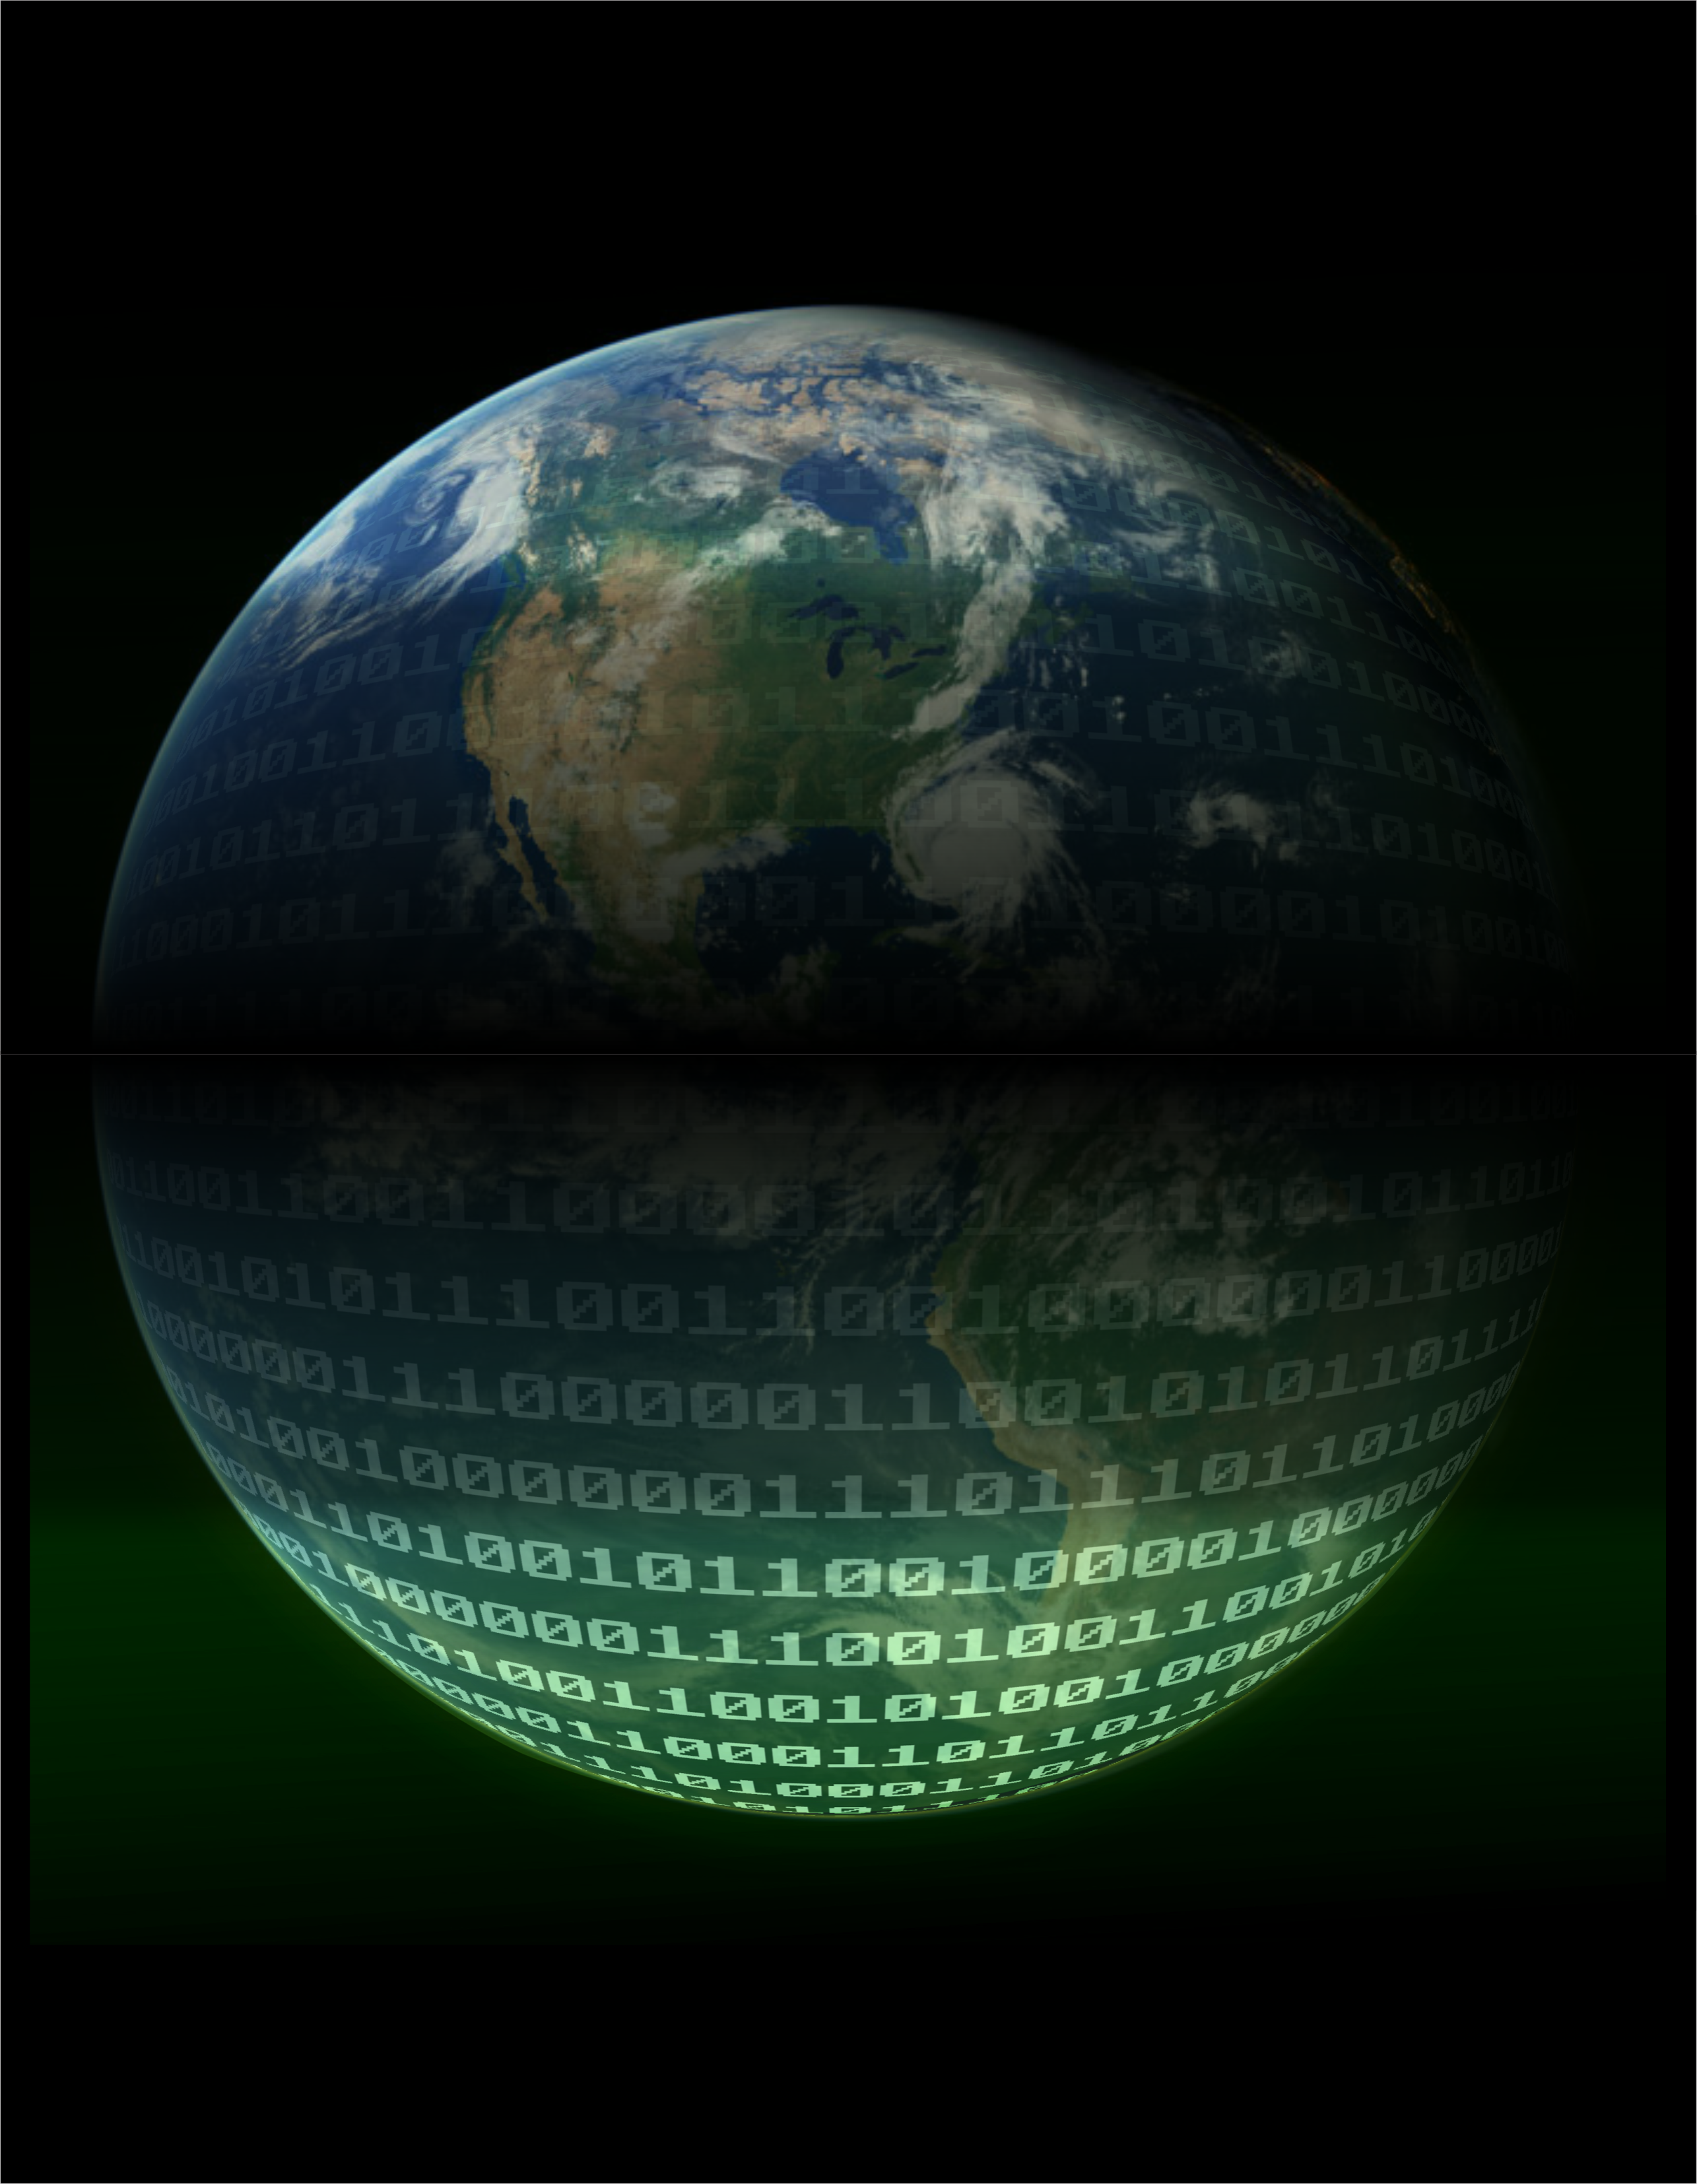
\includegraphics[scale=1.0]{cover}}} % Image background
\centering
\vspace*{7.5 cm}
\par\normalfont\fontsize{30}{30}\sffamily\selectfont
\textcolor[rgb]{1,1,0}{The Bumper Book of \textit{.cookie}s}\par % title
\vspace*{0.5cm}
\par\normalfont\fontsize{21}{21}\sffamily\selectfont
\textcolor[rgb]{0,0,1}{(The \textit{c}GENIE.cookie user-manual and introduction to Earth system modelling)}\par % title2
\vspace*{1cm}
{\Huge \textcolor[rgb]{1,1,1}{Andy Ridgwell}}\par % Author name
\endgroup

~\vfill
\textcolor[rgb]{1,0,0}{\today}

%----------------------------------------------------------------------------------------
%       COPYRIGHT PAGE
%----------------------------------------------------------------------------------------

\newpage
~\vfill
\thispagestyle{empty}

\noindent Copyright \copyright\ 2017 Andy Ridgwell\\ % Copyright notice

\noindent \textsc{Published by Derpy-cookies INC.}\\ % Publisher

\noindent \textsc{mycookie.seao2.org}\\ % URL

\noindent Licensed under the Creative Commons Attribution-NonCommercial 3.0 Unported License (the ``License''). You may not use this file except in compliance with the License. You may obtain a copy of the License at \url{http://creativecommons.org/licenses/by-nc/3.0}. Unless required by applicable law or agreed to in writing, software distributed under the License is distributed on an \textsc{``as is'' basis, without warranties or conditions of any kind}, either express or implied. See the License for the specific language governing permissions and limitations under the License.\\ % License information

\noindent \textit{First printing, October 2017} % Printing/edition date

%----------------------------------------------------------------------------------------
%       TABLE OF CONTENTS
%----------------------------------------------------------------------------------------

\chapterimage{courseimages.png} % Table of contents heading image

\pagestyle{empty} % No headers

\tableofcontents % Print the table of contents itself

\cleardoublepage % Forces the first chapter to start on an odd page so it's on the right

\pagestyle{fancy} % Print headers again

\mainmatter

%----------------------------------------------------------------------------------------
%----------------------------------------------------------------------------------------

%%----------------------------------------------------------------------------------------
%----------------------------------------------------------------------------------------
%       CHAPTER 00
%----------------------------------------------------------------------------------------
%----------------------------------------------------------------------------------------

\cleardoublepage

\chapterimage{muffin_planet.jpg} % Chapter heading image

\setcounter{chapter}{-1}
\chapter{Installation, Configuration, Basic Usage}

\hfill \break

%------------------------------------------------
\newpage
%------------------------------------------------

\section{(none)}

%----------------------------------------------------------------------------------------
%----------------------------------------------------------------------------------------
%----------------------------------------------------------------------------------------
%----------------------------------------------------------------------------------------
%       CHAPTER 00
%----------------------------------------------------------------------------------------
%----------------------------------------------------------------------------------------

\cleardoublepage

\chapterimage{muffin_planet.jpg} % Chapter heading image

\setcounter{chapter}{-1}
\chapter{Installation, Configuration, Basic Usage}\label{ch:0}

\hfill \break

\vspace{16mm}

\noindent Stuff to keep in mind:

\vspace{2mm}

\begin{itemize}
\item \textbf{(cGENIE.)cookie} is a \uline{model}. Models ARE NOT the ‘real World’. (Don’t get confused!)
\item The  low resolution (for a 3-D ocean circulation model) of the \textbf{cookie} model limits its applicability for very short time-scale problems.\ In configurations not incorporating the \textbf{PLASIM} atmospheric GCM component, there are no atmospheric dynamics or inter-annual variability in the coupled ocean-atmosphere system.
\item \textbf{cookie} is best thought of as a ‘discovery and exploring’ tool for learning how the Earth system has functioned in the past rather than a detailed ‘simulation’ tool for the future.
\item It is possible to have fun.
\end{itemize}

%------------------------------------------------
\newpage
%------------------------------------------------

\section{Before anything else …}

%------------------------------------------------

\subsection*{ReadMe}

Some warnings and reminders in this manual are repeated over and over and over and … over again.
Some warnings and reminders are repeated over and over and over and … over again.
This is because you will forget immediately each time! ;)
\\\textbf{!}\footnote{\textbf{Also read footnotes please.}}

%------------------------------------------------

\subsection*{Software version naming conventions}

You will be using the current version of the cGENIE Earth system model, code-named ‘\textbf{cookie}’ (if \textbf{Apple} can have ‘Leopard’, ‘Lion’ etc., I can have a baked goods version naming convention). The documentation may not be fully consistent in this respect … and you may need to translate occurrences of e.g. a directory named ‘\texttt{cgenie}’ to ‘\texttt{cgenie.cookie}’. For brevity, the \textbf{cGENIE.cookie} model will be referenced by just ‘\textbf{cookie}’.

%------------------------------------------------

\subsection*{linux ...}

The \textbf{(cGENIE.)cookie} model currently naively compiles and runs under \textbf{linux}\footnote{For some of you, the mechanics of running the model will be about as much fun as sticking your tongue in an electrical outlet (a popular hobby in England). (However, if you are an experienced linux/unix/tongue-in-electrical-socket user, you can skip onto the next Section and save yourself an entire 15 seconds of reading words.)} (e.g. distributions such as \textbf{Ubuntu}) and unix-like operating systems (such as \textbf{macOS}). \textbf{cookie} (like most climate models) is configured and accessed (aka ‘run') at the ‘command line’ of the linux (or \textbf{macOS} equivalent, which is unix-like) operating system. The command line is a place where you type text and when you press \small\textsf{Return}\normalsize, something (hopefully, good!) happens. Typically the stuff you type started with a ‘command’ word, and often followed by one or more options and parameters. The command word and any options / parameters MUST be separated by SPACEs.

The start of each line of the command line is indicated with something like: \texttt{\$}. The \texttt{\$} is called the ‘prompt’ and is ... prompting you to type some input (commands, Tweets, swear words, etc.). See – the computer is just sat there waiting for you to command it to go do something (stupid?). Typically, you will also be informed (reminded) of the user-name, computer name, and current directory, e.g.:

\vspace{-2mm}
\begin{verbatim}
[username@host ~]$
\end{verbatim}
\vspace{-2mm}

\noindent which is in this example is user ‘\texttt{username}’ (yours will be different!) on computer name ‘\texttt{host}’\footnote{Sprout the cat will eventually appear under ‘cat-of-the-day’ on my home-page if you press \textsf{F5} enough times – all my computing clusters are named after my cats …} and the current directory is the ‘home’ directory -- represented by the \texttt{\~} symbol. If, for example, you were instead currently in the \texttt{myfolder} directory, you would see at the command prompt something like:

\vspace{-2mm}
\begin{verbatim}
[username@host myfolder]$
\end{verbatim}
\vspace{-2mm}

If you are not or not very familiar with the linux/unix command line, such as how to navigate up and down the directory tree and to display the contents of the current directory you are in – for a brief summary of some basic/useful \textbf{linux} commands and usage -- see the linux HOW-TO Section towards the back of the book.

NOTE: BE VERY CAREFUL that spaces are not missed out when typing out example lines. Also be careful not to confuse the number one (\texttt{1}) for the letter 'el' (\texttt{l}). Mis-spelling/typing is generally the most likely reason for things not working.

NOTE-the-second: If you find yourself terminally bored typing in long long instructions lines, you may be tempted to simply copy-paste from the cookie manual PDF to the command line, This can work, but firstly be aware that trying to copy-paste multiple lines at once is doomed to failure -- copy-paste the first line and then following that add the second (or subsequent) line.
Also note that the inverted comma symbol in the PDF is not the same inverted comma symbol that linux is expecting ... You should also make liberal use of the up arrow key that bring back the previously entered command (keep pressing the key for progressively older commands). For instance, a mistake in a command line can be corrected by bringing back the offending line and using the left/right arrows to navigate through the characters and correct any mistake.

NOTE-the-third: In places, instructions may be given for specific programs and computer platforms and hence may differ slightly from the software reality in front of you. Use your judgement in translating such instructions. Many other alternative software choices exist for editing files or viewing results, as are other ways of configuring software and file editing/transferring methodologies. Do what suits you best – you can view such instructions where they occur, as  more representing an example methodology rather than a literal interpretation of the Constitution.

%------------------------------------------------

\subsection*{Required computer hardware/software}

For running \textbf{cupcake}, your options are:

\begin{enumerate}[noitemsep]

\vspace{1mm}
\item \textbf{Remotely}
\\To do this, you will need an account on a linux-based server or cluster. You can use any platform (\textbf{linux}, \textbf{macOS}, \textbf{Windoz}, as well as \textbf{iOS} and \textbf{Android} (which is based on \textbf{linux} in any case)) to connect to the cluster. You will need the following software on your local machine:
\vspace{1mm}
\begin{enumerate}[noitemsep]
\setlength{\itemindent}{.2in}
\item A terminal (‘shell’) window. This is no problem for \textbf{linux} and \textbf{Mac} users (you already have one built in). For \textbf{Windows}, either download a simple (and old) \textbf{SSH} client (ssh-client) from my website\footnote{http://www.seao2.info//cgenie/software/ssh-client.exe} or you can get hold of e.g. \textbf{PuTTY} (http://www.putty.org/).
\item A sftp (secure file transfer) client for convenience (i.e. dragging and dropping files between local and remote computers, and opening files directly on the remote computer cluster). If you have installed ssh-client (\textbf{Windows}, above) then a sftp client is already included as part of this software. If using \textbf{PuTTY} (\textbf{Windows}) you might try downloading \textbf{WinSCP} (http://winscp.net/eng/index.php). For \textbf{macOS}, you can connect to the server through the \textbf{Terminal}, but some sftp software for viewing/navigating server file structure include: \textbf{FileZilla} (recommended), \textbf{Cyberduck}, \textbf{TextWrangler}. For linux, maybe \textbf{FileZilla}.
\end{enumerate}

\vspace{1mm}
\item \textbf{Locally}
\\It is  possible to install and run the ‘\textbf{(cGENIE.)cookie}’ Earth system model either on a linux box (e.g. \textbf{Ubuntu}) or on a \textbf{Mac} \footnote{Sets of detailed installation instructions are available in the HOW-TO section of this manual.}\footnote{It is also possible to run \textbf{cookie} under \textbf{Windows}.}. At a minimum, you will need:
\vspace{1mm}
\begin{enumerate}[noitemsep]
\setlength{\itemindent}{.2in}
\item A FORTRAN (f90 and f77 combatable) compiler of some sort.
\\This may come with the operating system as standard, possibly \textbf{gfortran}.
\item A \textbf{git} client.
\\If not standard, this is relatively easy to add and install.
\item Compiled \textbf{netCDF} libraries (not so much fun ...).
\end{enumerate}
\vspace{1mm}
To edit files and visualize results, you will need some specific software. The exact software will depend on your operating system, but essential are:
\vspace{1mm}
\begin{enumerate}[noitemsep]
\setlength{\itemindent}{.2in}
\item A viewer for netCDF format spatial data. A \textbf{Java} viewer called \textbf{Panoply} is provided by NCAR for all platforms – http://www.giss.nasa.gov/tools/panoply/
(Note that you will need \textbf{Java} installed!) (Or alternatively: \textbf{MATLAB}, \textbf{python}, etc..)
\item  A simple text editor, except not the rubbish default \textbf{Windows} one – you need one that can display \textbf{unix} ASCII text without screwing it up. Options for \textbf{Windows} users are:
\textbf{notepad++} (https://notepad-plus-plus.org/)
\textbf{SciTE} (https://www.scintilla.org/SciTE.html)
(\textbf{linux} and \textbf{Mac} users need no special/different editor compared with your standard editor – everything will display just fine). You can also use \textbf{linux} command line based editors such as \textbf{vi}.
\end{enumerate}
\vspace{1mm}

\end{enumerate}
\vspace{1mm}

%------------------------------------------------

\subsection*{File editors ...}

You will need to edit text-based configuration files, possibly in installing and configuring \textbf{cookie}, but definitely in configuring model experiments. So now might be a good time to check that you can use the/an editor! (You will also be using the same editor to view some of the model output.)

You have two alternative options for editing and viewing text files, depending on whether you are a \textbf{unix} nerd with no life, or prefer anything to do with computers to be wrapped in cotton wool and covered with dollops of treacle.
EITHER: Use the linux \textbf{vi} (/\textbf{vim}) application (or similar e.g. \textbf{emacs}) if you are familiar with it. I think that this pretty much sucks as a text editor and life is far too short and brutal if you don't like this sort of thing … OR ... use a suitable linux-friendly text editor (NOT \textbf{Micro\$oft} \textbf{Notepad}) in conjunction with the \textbf{Secure File Transfer Client}. For example: \textbf{SciTE} (http://www.scintilla.org/SciTE.html) is suitable, or \textbf{Notepad++}.

If you fiddle about with the settings under Options/Preferences in the \textbf{WinSCP} program and apply a little common sense, it should be possible to configure things so that you can simply double-click on a file in the remote (right-hand) window panel and it will open like magic (almost)! Saving the file after editing) should then result in the file being saved back to the cluster. Or you can select Edit With (and then \textbf{SciTE}) from right-mouse-button-clicking on the filename. Or ... a crude but workable approach is to use an sftp client to drag the file to your local machine (assuming \textbf{cookie} is installed remotely), edit it there, and then drag it back again.\footnote{Note that care still has to be taken to avoid certain \textbf{Microsoft} text editing programs under \textbf{Windoz}.)}

%------------------------------------------------
\vspace{1mm}\noindent\rule{4cm}{0.5pt}\vspace{2mm}
%------------------------------------------------

%------------------------------------------------
\newpage
%------------------------------------------------

\subsection*{Model documentation in general}

This (the \textbf{cookie} manual), and additional documentation (of varying degrees of up-to-date-ness) can be found:

\vspace{1mm}
\begin{enumerate}[noitemsep]
\setlength{\itemindent}{.2in}
\item On \href{https://github.com/genie-model/cookiedoc}{GitHub}.
\\The \textbf{latex} source for the documentation lives here, allowing you to compile the most up-to-date PDF document. And ... make changes yourself and have them incorporated into the official documentation\footnote{First clone the \textbf{git} repository. Make changes. Commit them locally. Make a 'pull request' ...}.
\\However, note that you will have to compile the latex source yourself to create a PDF ...
\item On my \href{http://www.seao2.info/mymuffin.html}{website}.
\\Here you can find compiled PDF versions of the documentation ... but it could be a little out of date (the up-to-date latex sources lives on \textbf{GitHub}).
\end{enumerate}

%------------------------------------------------

\subsection*{This document in particular}

The instructions  may not be entirely bug-free -– use your judgment.

%------------------------------------------------

\subsection*{Go!}

OK – now we are ready to start …

%------------------------------------------------
\newpage
%------------------------------------------------

\section{Starting (dozing?) off …}

You are going to be installing the model from scratch – why? Why not? It will be a happy character-building experience for you ... trust me ...

%------------------------------------------------

\subsection{Logging in!}

In running \textbf{cookie} locally -- log into your \textbf{linux}/\textbf{macOS} box (and skip on to the next section)! \footnote{If you fail at this step, you'll have to take up box-modelling instead.}

\noindent Or ... and much more likely to be the case -- if you are running \textbf{cookie} \uline{remotely} (e.g. via a user account on a computing cluster or server), then log into the remote server or cluster account using a 'suitable terminal program'\footnote{It very much depends on what software you are using. Provided are instructions for some \uline{examples}, but only examples, and your reality may be rather different.}:

\begin{itemize}
\vspace{1mm}
\item If logging in via a \textbf{linux}/\textbf{macOS} box, open the terminal/shell window and simply SSH in\footnote{If your current directory looks something like this: \texttt{[username@clustername \(\sim\)]\$}
then you are probably already logged in! Otherwise, it will look like: \texttt{username@localcomputername:\(\sim\)\$}}, e.g.

\vspace{-1mm}
\begin{verbatim}
$ ssh username@clustername
\end{verbatim}
\vspace{-1mm}

where \texttt{clustername}, the cluster (or remote server) name(!) might, for example, be
\\\texttt{catname.ucr.edu}, and enter your  account password (and tell it whether or not you want this password stored, if asked).
\vspace{1mm}
\\\textbf{IMPORTANT!} -- When you type in a password in \textbf{linux}, NOTHING appears on the screen, not even \texttt{********} as in common on \textbf{Windoz}. As you type (the password), characters are being entered ... you just cannot see them. Don't panic -- just type in the password (even if you cannot see characters appearing) and hit \textsf{\scriptsize Enter}.

\vspace{1mm}
\item On a \textbf{Windoz} machine – first start the \textbf{WinSCP} program (an sftp file transfer client). Under \textsf{\footnotesize Host Name}, enter the remote server or cluster name (e.g. \texttt{catname.ucr.edu}):
\\The \textsf{\footnotesize Port number} should be set to \textsf{\footnotesize 22} (except for \texttt{sterling.ucr.edu}). Enter your computing cluster user-name on the line below this (‘\textsf{\footnotesize User Name}’) and then the \textsf{\footnotesize Password}. Click on \textsf{\footnotesize Login}.
\\You will also need a terminal window. This can be opened by clicking on the ‘\textsf{\footnotesize Open session in PuTTY}’ icon on the top icon row, or pressing \textsf{\footnotesize Ctrl+P}. \\You should now have TWO windows open – a ‘shell’ window (lines of text on an otherwise blank screen) and a file manager (transfer) window. Ensure that you have both these before moving on. It is recommended that you maximize both these windows to full screen. (But no-one will die horribly for not doing so. Probably ...).
\\ You can also log in directly from the shell/terminal window e.g. \textbf{PuTTY} first (rather than first opening an sftp connection first).
 You will sill have to open an sftp connection for file transfer.
\end{itemize}

\vspace{1mm}
Note that the cluster you access may not use the standard 'port' number of \textsf{\footnotesize 22}. If your computer uses a different port number -- in the login window of your sftp client, simply change the number in the \textsf{\footnotesize Port} box, or if you are using the command line, you will need to type:
\vspace{-1mm}
\begin{verbatim}
$ ssh -p xxxxx username@clustername
\end{verbatim}
\vspace{-1mm}
where \textsf{\footnotesize xxxxx} is the port number.

%------------------------------------------------

\subsection{Downloading/installing the model code}

The next step is to download/install a copy of the source code for \textbf{cookie}. The current release of the \textbf{cGENIE} model (\textbf{cookie}) lives here:

\vspace{1mm}
\href{https://github.com/genie-model/cgenie.cookie}{\texttt{https://github.com/genie-model/cgenie.cookie}}
\vspace{2mm}

There are 2 options:

\begin{enumerate}

\vspace{1mm}
\item '\textbf{cloning}'
\\The \uline{preferred/advised} way is to \textit{clone} the repository to where you intend to run \textbf{cookie}\footnote{But see later for other/better ways of working.}. While you can also use a GUI based git client, easiest is at the command line (e.g. from your HOME directory), using the command \texttt{git clone}\footnote{This: "... clones a repository into a newly created directory, creates remote-tracking branches for each branch in the cloned repository, and creates and checks out an initial branch that is forked from the cloned repository’s currently active branch."}:
\vspace{-1mm}
\begin{verbatim}
$ git clone https://github.com/genie-model/cgenie.cookie.git
\end{verbatim}
\vspace{-1mm}

By doing this, you have created your own code repository (and an identical copy of the one hosted on GitHub). As part of the \texttt{git clone} command, you also automatically \textit{check out} (from your very own personal repository) a copy of the code. \footnote{Note that the major difference then with the \textbf{svn} system, is that previously, the GENIE code repository existed only on the University of Bristol server, and you \textit{checked out} the code remotely from there.}

\vspace{1mm}
\item Simple downloading.
\\\uline{Less good}, but OK if you simply want a copy of the code to run an experiment just once, or simply only want to see the code.) By downloading an archive file, containing all the code etc. For this -- click on the \textcolor[rgb]{0,0.501961,0}{green} \textsf{\footnotesize Clone or Download} button on \textbf{GitHub}, and select \textsf{\footnotesize Download ZIP}. You then unpack/unzip the files and directory structure where you want it. This [archive download] is a perfectly workable way to proceed ... as long as you neither want to update the code with whatever new developments or bug fixes occur in the future, nor want to have any code changes you might make, become part of the official \textbf{cookie} code  (i.e. it becomes a one-off installation that has no connection to the \textbf{GitHub} repository.

\end{enumerate}

%------------------------------------------------

\subsection{Configuring the code}

\noindent You may ... or may not, need to configure some local environment settings so that all the libraries etc. that are needed to compile \textbf{cookie} can be found. To a very limited extent, cookie will try and identify your computer and make the required setting automatically. The changes, if any, that you need to make will depend on the platform where you will be running \textbf{cookie} (i.e. the computer where you have just cloned (or downloaded) the code repository to). The currently recognized platforms and required actions are as follows:

\vspace{1mm}
\noindent The required configuration settings for \textbf{cookie} depend on the specific computing platform that you are running on. What follows is a list of the changes associated with some possible platforms that you might be using -- \uline{find the list name (\textbf{bold}) that corresponds to the platform that you are using} and ignore all the other options.\footnote{If you are using a platform not listed here, you may be able to simply adapt the instructions for one of the ones listed.}

%------------------------------------------------
\newpage
%------------------------------------------------

\begin{itemize}

\vspace{1mm}
\item \textbf{Ubuntu} -- no changes are necessary (with caveats).
\\ This is the default assumed platform. No changes are necessary IF the \textbf{netCDF} libraries are installed in their default locations and a relatively recent version of \textbf{netCDF} is used.\footnote{By 'relatively recent' -- the default settings assume that the \textbf{FORTRAN} and \textbf{C} \textbf{netCDF} libraries are separate.}

\vspace{1mm}
\item \textbf{sterling} (UCR cluster) -- no changes are necessary (the cluster is automatically identified).

\vspace{1mm}
\item \textbf{eevee} (UCR cluster) -- no changes are necessary (the cluster is automatically identified).

\vspace{1mm}
\item \textbf{macOS}
\\ Please refer to the separate \textbf{macOS} instructions.

\vspace{1mm}
\item \textbf{Windows} 
\\ Please refer to the separate \textbf{Windoz} instructions.

\vspace{1mm} 
\item \textbf{Otherwise} ...
\\... one or more edits will be required to the file \textsf{\footnotesize user.mak}, which lives in the \textsf{\footnotesize genie-main} directory.

\begin{enumerate}[noitemsep]
\vspace{2mm}
\item At the end of the \textsf{\footnotesize user.mak}, the \textbf{netCDF} path needs to be changed.
\vspace{1mm}  
\\First comment out\footnote{To 'comment out' a line -- simply add a \texttt{\#} symbol to the very start of the line. When \textbf{cookie} runs, this line will be ignored.}. i.e.,
\small\begin{verbatim}
  ### DEFAULT ###
  NETCDF_DIR=/usr/local
\end{verbatim}\normalsize
to
\small\begin{verbatim}
  ### DEFAULT ###
  #NETCDF_DIR=/usr/local
\end{verbatim}\normalsize
Then un-comment\footnote{To 'un-comment' a line -- simply remove (delete) the \texttt{\#} symbol from the beginning of the line.} the line: \texttt{\#NETCDF\_DIR=my\_path}
\\\uline{AND} change \texttt{my\_path} to be the path to your \textbf{netCDF} libraries ... the trick step :o)

\vspace{2mm}
\item For MacOS users, there are alternative machine type options depending on your CPU. You need to comment out \texttt{MACHINE=LINUX} in  \textsf{\footnotesize user.mak} and then chose and un-comment one of the following:
\small\begin{verbatim}
#MACHINE=OSX	# Intel processor
#MACHINE=OSX_M	# Apple silicon (M1, M2 etc.)
\end{verbatim}\normalsize

\end{enumerate}

\end{itemize}

%------------------------------------------------
\vspace{1mm}\noindent\rule{4cm}{0.5pt}\vspace{2mm}
%------------------------------------------------

\noindent If your computer is configured to use python v.2 by default and/or does not have python v.3, then you will need to make a few minor changes (see HOW-TO).

%------------------------------------------------
\newpage
%------------------------------------------------

\subsection{Testing the model code}

\noindent Finally, you need to test the code to ensure that all the files have been cloned/installed correctly.

\vspace{1mm} 
\noindent First, change directory (see: Figure \ref{fig:directories}, and refer to the linux HOW-TO) to\footnote{Note: the model is *always* run from \texttt{cgenie.cookie/genie-main}}:
\vspace{-2mm}\begin{verbatim}
cgenie.cookie/genie-main
\end{verbatim}\vspace{-2mm}

\noindent If you are not ‘linux-friendly’ (see: Section \ref{how-to-linux} for \textbf{linux} basics) – maybe at first do this in steps – list the contents of the directory (\texttt{ls}) to check where you are (i.e. what directories are available to chance to), then change to \texttt{cgenie.cookie} (\texttt{cd cgenie.cookie}), then list again (\texttt{ls}) (and see what further directories are there), then change to \texttt{genie-main} (\texttt{cd genie-main}), and only then … type\footnote{Remembering that the \texttt{\$} is to indicate the command line, and you do not actually type it in.}:
\vspace{-2mm}\begin{verbatim}
$ make testbiogem
\end{verbatim}\vspace{-2mm}

\noindent This compiles a basic carbon cycle enabled configuration of \textbf{cookie} and runs a short test, comparing the results against those of a pre-run experiment (also downloaded alongside the model source code). It serves to check that you have the software environment correctly configured. There may be some ’Warnings’ reported (== somepony’s sloppy programming) but these are not detrimental to the ultimate science results (we hope!).
\vspace{1mm}
If you see the error message:
\vspace{-2mm}\begin{verbatim}
make: *** No rule to make target 
\end{verbatim}\vspace{-2mm}
when you try this, you are probably in the wrong directory (it should be \textsf{\footnotesize cgenie.cookie/genie-main}).

%------------------------------------------------
\vspace{1mm}\noindent\rule{4cm}{0.5pt}\vspace{2mm}
%------------------------------------------------

\noindent ‘Success’ of this test is indicated by the message:
\vspace{-1mm}
\small\begin{verbatim}
**TEST OK**
\end{verbatim}\normalsize
\vspace{-1mm}

\noindent If you see this -- you can then be certain that the model you have installed is producing identical (within tolerance) results to everyone else in the World who has ever installed \textbf{cookie}. Note that the model will pause for a l o o o o n g time at the line:
\vspace{-2mm}
\small\begin{verbatim}
./genie.job -t -k -f configs/eb_go_gs_ac_bg_test.xml -o /home/genie00/cgenie_output
   -c /home/genie00/cgenie -g ../../cgenie -m "" > testbiogem.out;
\end{verbatim}\normalsize
\vspace{-2mm}

\noindent This is quite ‘normal’ – the model is thinking! Also -- ignore the compiler warnings … 

\vspace{1mm}
\noindent \uline{This completes the basic code installation.}

\vspace{1mm}
\noindent If the test doesn't 'work'\footnote{Note that if you have disabled the compilation of the C program that compares netCDf files, the test will run but never complete and you'll not get a \texttt{**TEST OK**} reported, even if the test experiment ran correctly.} -- try issuing the command:
\vspace{-2mm}\begin{verbatim}
$ make cleanall
\end{verbatim}\vspace{-2mm}

\noindent and then re-try the test. 

\vspace{1mm}
Refer to the FAQ section at the end of this book for further clues as why the model installation appears not to be working.

%------------------------------------------------
\newpage
%------------------------------------------------

\noindent Note that \textbf{GitHub} does not host files larger than 100 MB, and the 'lookup table' for calculating opal dissolution in sediments (see e.g., \textit{Ridgwell et al.} [2003]) is larger than this. It has hence been committed to \textbf{git} as an archived file. \uline{Only if} a silica cycle is to be employed in your \textbf{cookie} experiments, does this file need to be unpacked. A script is provided for this -- from \texttt{genie-main}, type:

\vspace{-2mm}
\begin{verbatim}
$ ./installcookie.sh
\end{verbatim}
\vspace{-2mm}

\noindent and this will unpack the opal lookup table to \texttt{genie-sedgem/data/input} as well as unpacking a copy of the calcium carbonate lookup table\footnote{For now, the \(CaCO_{3}\) lookup table also included in the git repo in its expended (unpacked) form.}.

%------------------------------------------------
\vspace{1mm}\noindent\rule{4cm}{0.5pt}\vspace{2mm}
%------------------------------------------------

\subsubsection*{Some brief notes on git}

The simplest workable installation of \textbf{cookie}, as described above, is to use \texttt{git clone}. You end up with a carbon copy of the cookie code repo (I am too lazy to type out 'repository' again) which you have also automatically now 'checked out'. Changes and developments will occur to the code on the GitHub repo from time-to-time, and if may be that either you might benefit by using a more up-to-date code base, or specific changes may have been made that you absolutely need. To determine the status of your repo, type\footnote{Here, the -uno ensures that files (e.g. experiment configuration files) you have created, but not added and committed, are not listed.} (from \texttt{cgenie.cookie}):

\vspace{-2mm}
\begin{verbatim}
$ git status -uno
\end{verbatim}
\vspace{-2mm}

\noindent However, git has not actually compared your repo with the one on GitHub, because this is apparently network expensive (as if you don't spend the rest of your life killing the internet by streaming Rick and Morty). So, use:

\vspace{-2mm}
\begin{verbatim}
$ git fetch
\end{verbatim}
\vspace{-2mm}

\noindent which will 'download [new and modified] remote content but not update your local repo's working state'. If you now type \texttt{git status -uno}, \textbf{git} can tell you if there is newer content (e.g. '\texttt{Your branch is behind 'origin/master}'\footnote{\texttt{origin} is the origin of the repo -- GitHub, and \texttt{master} is the name of the branch, in this case, the default branch name.}). To merge in the fetched content:

\vspace{-2mm}
\begin{verbatim}
$ git merge
\end{verbatim}
\vspace{-2mm}

Both these commands are also combined in a single command\footnote{If there are no changes (to \textit{fetch} and \textit{merge}), the you get the message: \texttt{Already up-to-date.}}:

\vspace{-2mm}
\begin{verbatim}
$ git pull
\end{verbatim}
\vspace{-2mm}

If you are not developing code, and hence not editing files in the repo (but e.g. only adding new model configuration files), your life should mostly be trouble-free with regards to updating your code via \texttt{pull}.\footnote{
One exception is, if any of the model installation/configuration files that you might have edited, i.e. one or all of: \texttt{genie-main/user.mak}, \texttt{genie-main/makefile.arc}, and/or \texttt{genie-main/makefile}, have also changed on \texttt{origin/master}, then \texttt{pull} (or \texttt{merge}, after \texttt{fetch}) will fail (with the message: '\texttt{Please, commit your changes or stash them before you can merge. Aborting}'). The root issue is a conflict between remote file changes, and local ones that you had not committed to your repo.

You probably want to keep your local configuration changes, otherwise you'll probably end up re-doing them all over again. One solution is to sneakily 'hide' (\textit{stash}) them out of sight, by:
\$ git stash
\noindent You can now pull, updating your repo with respect to \texttt{origin/master}. Then -- you want your changes back, so apply the stashed changes:
\$ git stash apply
If unlucky, there will be conflict as your stashed changed are merged back onto your local repo branch (master). If so, you'll need to edit the file, deciding which line(s) is correct, and delete the version you do not want, along with the ASCII tags/labels.
}

%------------------------------------------------

\begin{figure}
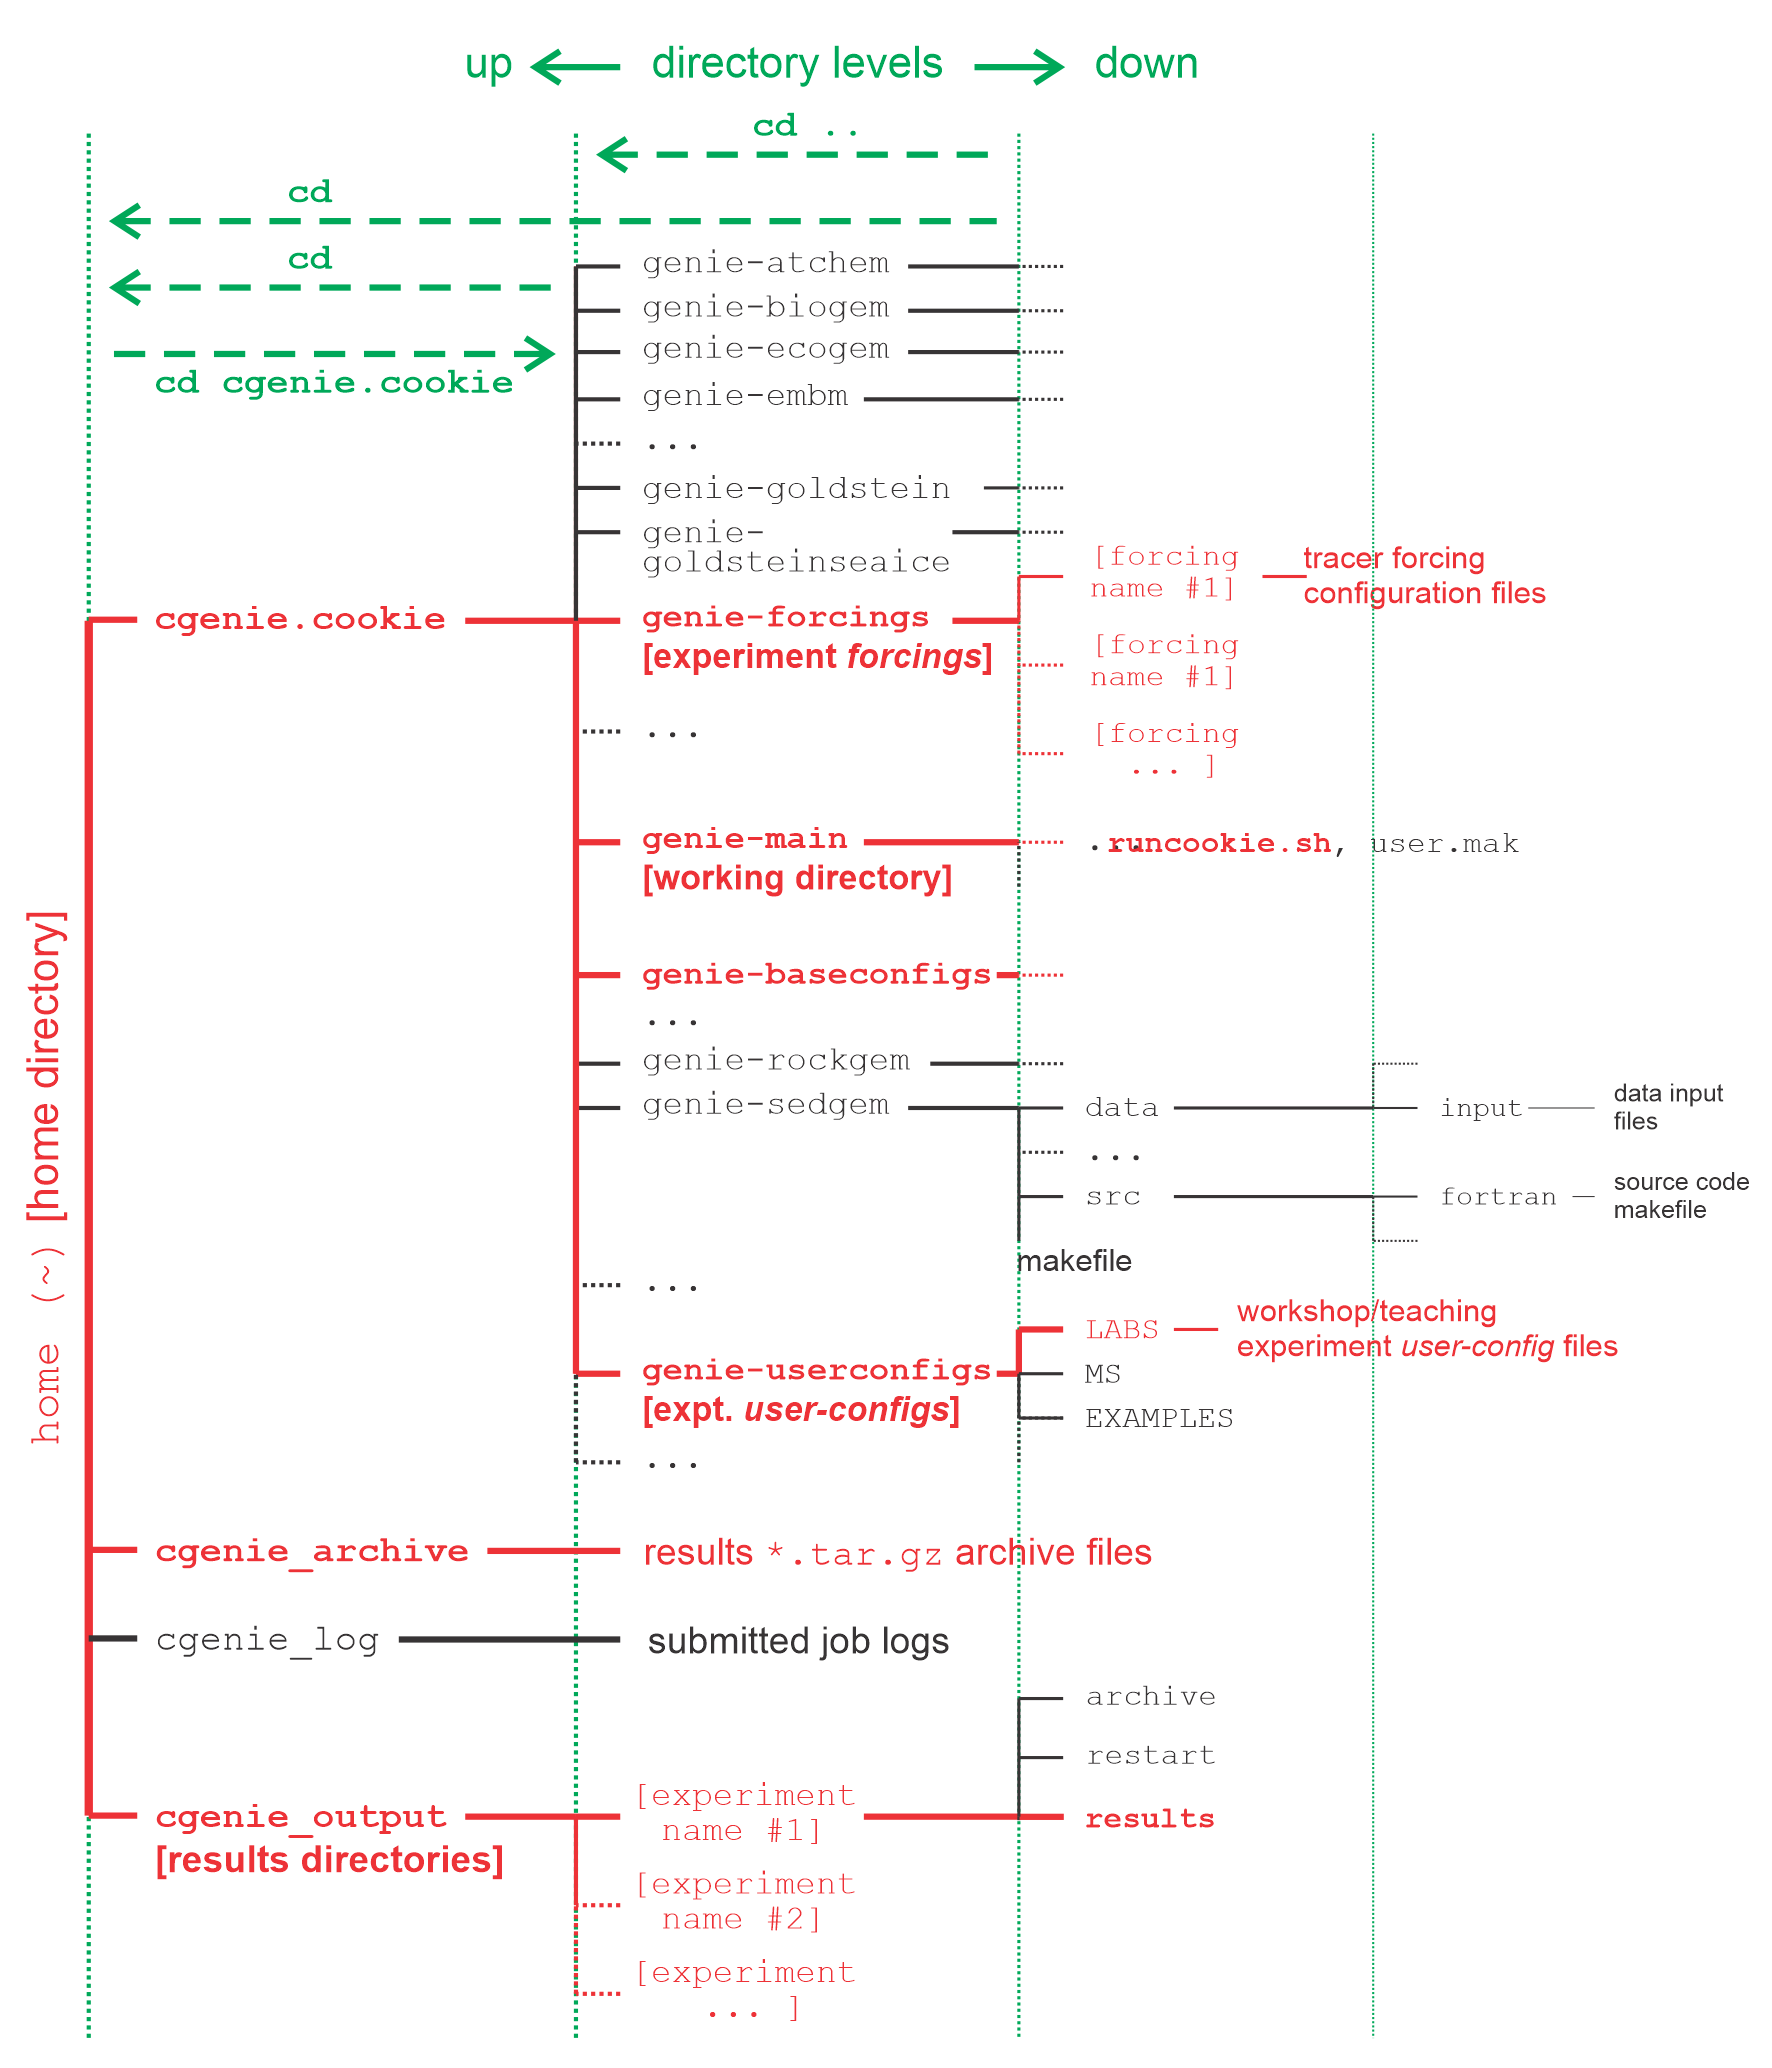
\includegraphics[width=\linewidth]{Figures.usermanual.1.png}
\caption{Directory structure of the \textbf{cookie} model. Highlighted in \textcolor{red}{red} are directories and sub-directories that you will need to access at some point. Vertical \textcolor[rgb]{0,0.501961,0}{green} lines designate directory levels, with example commands shown for moving between them.}
\label{fig:directories}
\end{figure}

%------------------------------------------------
\newpage
%------------------------------------------------

\section{Running the model}

The overall sequence of configuring and running \textbf{cookie} (job submission to a cluster queue), is shown in Figure \ref{fig:chx-jobcreation}. Refer to this if in any doubt at any point.

At the command-line (\texttt{\$}) and \uline{in the \textsf{\footnotesize genie-main} directory} (not your home directory), you will be entering in a command (\texttt{./runcookie.sh}) together with a list of parameters that will be passed to the model, and as if by magic the model will run (or sometimes not). The form of the command you are going to be issuing is:

\vspace{-1mm}\begin{verbatim}
$ ./runcookie.sh #1 #2 #3 #4 (#5)
\end{verbatim}\vspace{-1mm}

\noindent(\uline{don't type it yet}!) It requires that you must list at least 4 parameters after \texttt{./runcookie.sh}, separated by S P A C E S and on a single continuous line (even if it ‘wraps’ around across 2 lines of the screen).
These parameters are:

\vspace{2mm}
\begin{enumerate}[noitemsep]
\setlength{\itemindent}{.2in}
\item[\textbf{\#1}] ... is the name of the required base (or ‘basic’) configuration (‘\textit{base-config}’) of the model.
\item[\textbf{\#2}] ... is the name of the subdirectory (if any) containing the user configuration (‘\textit{user-config}’) file (i.e., the file containing the specification of a particular experiment).
\item[\textbf{\#3}] ... is the name of the experiment itself. There must exist a file in the directory specified by parameter \#2 (\texttt{LABS}) with exactly the same name as you enter here for parameter \#3 (i.e. parameter \#3 points to a file in the directory given by parameter \#2).
\item[\textbf{\#4}] ... is the run length of the experiment in years – this must be entered as an integer.
\item[\textbf{(\#5)}] ... There is also one optional (5th) parameter (to be described later).
\end{enumerate}

%------------------------------------------------
\vspace{1mm}\noindent\rule{4cm}{0.5pt}\vspace{2mm}
%------------------------------------------------

\noindent As an example of running the \textbf{cookie} Earth system model:

\vspace{2mm}
\begin{enumerate}[noitemsep]
\setlength{\itemindent}{.2in}
\item[\textbf{\#1}]: The \textit{base-config} is: \texttt{cookie.CB.p\_worbe2.BASES}
\item[\textbf{\#2}]: The \textit{user-config} directory is: \textsf{\small LABS}
\item[\textbf{\#3}]: The \textit{user-config} file (the experiment name) is: \texttt{LAB.0.3.EXAMPLE}.
\item[\textbf{\#4}]: Run the experiment for ten years: 10
\item[\textbf{\#5}]: (There is no restart file, and so no 5th parameter needs to be passed …)
\end{enumerate}

The full command for your first example experiment, which you are going to issue from the \texttt{\~}\texttt{/cgenie.cookie/genie-main} directory, then looks like:

\vspace{-1mm}\begin{verbatim}
$ ./runcookie.sh cookie.CB.p_worbe2.BASES LABS LAB.0.3.EXAMPLE 10
\end{verbatim}\vspace{-1mm}

\noindent(\uline{you can try it now}!)

\vspace{2mm}
\textbf{REMEMBER: This must be entered on a single CONTINUOUS LINE.}

\textbf{The (single) S P A C E S are vital. }

\textbf{ALSO -- take care not to confuse an el (‘\texttt{l}’) with a one (‘\texttt{1}’)  ... (it is a ‘one’ here).}

%------------------------------------------------
\newpage
%------------------------------------------------

\noindent What should happen is: First, you will end up twiddling your thumbs a while, as all the components of \textbf{cookie} are compiled from the raw source code (\textbf{FORTRAN}). When it has finished doing this, the model will initialize and carry out some brief self-checking. Only then will it start actually ‘running’ and doing something ... in this particular example, the output should look something like this:

\vspace{-2mm}\tiny\begin{verbatim}

 *******************************************************
  *** Initialisation complete: simulation starting ...
 *******************************************************

 >   model year |   pCO2(uatm)   SAT(oC) |   AMOC(Sv)    ice(%)   SST(oC)  SSS(PSU) |       pH  OHMEGA |   [O2](uM)  fPOC(PgC/yr)

 >          0.5 |      285.042    -3.667 |     12.715     0.274     1.408    34.902 |    8.048   2.537 |    181.360        12.327
 >          1.5 |      295.295    -2.531 |     13.189     2.126     3.450    34.902 |    8.079   2.896 |    191.671        12.636
 >          2.5 |      302.383    -1.270 |     12.266     4.282     5.004    34.904 |    8.088   3.131 |    196.879        12.394
 >          3.5 |      307.657    -0.274 |     11.020     5.525     6.214    34.906 |    8.093   3.318 |    199.930        12.216
 >          4.5 |      311.667     0.628 |      9.831     6.037     7.185    34.908 |    8.096   3.469 |    201.861        12.096
 >          5.5 |      314.811     1.437 |      8.876     6.387     7.987    34.910 |    8.099   3.597 |    203.157        11.994
 >          6.5 |      317.299     2.150 |      8.091     6.628     8.667    34.911 |    8.101   3.707 |    204.047        11.899
 >          7.5 |      319.290     2.782 |      7.872     6.673     9.256    34.913 |    8.103   3.800 |    204.669        11.822
 >          8.5 |      320.852     3.342 |      7.886     6.734     9.773    34.914 |    8.105   3.882 |    205.073        11.742
 >>> SAVING BIOGEM TIME-SLICE AVERAGE CENTERED @ year  :        9.500
 >          9.5 |      322.066     3.848 |      7.935     6.684    10.232    34.914 |    8.106   3.954 |    205.320        11.670

 *******************************************************
  *** Simulation complete: shutdown starting ...
 *******************************************************

\end{verbatim}\normalsize\vspace{-2mm}

%------------------------------------------------
\vspace{1mm}\noindent\rule{4cm}{0.5pt}\vspace{2mm}
%------------------------------------------------

\noindent What do all these numbers mean? From left-to-right:

\vspace{1mm}\begin{itemize}
\item[] \texttt{model year}  -- ... guess!
\end{itemize}\vspace{1mm}

\noindent Then:

\vspace{1mm}\begin{itemize}
\item[] p\(CO_{2}\)(uatm) -– mean atmospheric CO\(_{2}\) concentration (in units of \(\mu\)atm)
\item[] \texttt{<SST>} -- global mean surface air temperature ('SAT') $^{\circ}$C
\end{itemize}\vspace{1mm}

Note that if you are not running an experiment without a carbon cycle, there will be no values for p\(CO_{2}\).

\vspace{1mm}\begin{itemize}
\item[] \texttt{AMO(Sv)} -- Atlantic meridional overturning circulation (AMOC) (Sv)
\item[] \texttt{ice(\%)} -- global sea-ice fraction (\%)
\item[] \texttt{<SST>} -- global sea surface temperature ('SST') $^{\circ}$C
\item[] \texttt{<SSS>} -- global sea surface salinity ‘SSS’ (\%\textit{o})
\end{itemize}\vspace{1mm}

Note that if you are not running an experiment with a modern-like Atlantic basin, no value is given for the AMOC.

\noindent After that, a couple of carbonate chemistry indicators:

\vspace{1mm}\begin{itemize}
\item[] \texttt{pH} -- Mean ocean surface pH.
\item[] \texttt{OHMEGA} -- Mean ocean surface OHMEGA ...
\end{itemize}\vspace{1mm}

\noindent which will become apparent later.

Note that if you are not running an experiment without a carbon cycle, no values will be given.

\noindent Finally:

\vspace{1mm}\begin{itemize}
\item[] \texttt{O2} -- Dissolved oxygen in the ocean(global mean). ($\mu mol kg^{-1}$)
\item[] \texttt{fPOC} -- Global total annual export production (in terms of particulate organic carbon ($PgC yr^{-1}$).
\end{itemize}\vspace{1mm}

Note that you need some sort of biological pump in the ocean for these to be meaningful.

%------------------------------------------------
\vspace{1mm}\noindent\rule{4cm}{0.5pt}\vspace{2mm}
%------------------------------------------------

\noindent The choice of what information to display on screen as the model is running is rather arbitrary, but the chosen metrics do tend to summarize some of the main properties of the climate system and carbon cycle – for my own personal convenience rather than reflecting any fundamental scientific truth ... 

This information is reported at the same intervals as \textit{time-series} data (see later and/or refer to the User Manual) is saved and is indicated by:

Interleaved between these lines are lines reporting the saving of \textit{time-slice} data (the 2- and 3-D model states – more of which later as well as in the User Manual). These appear as:

\vspace{-2mm}\small\begin{verbatim}
>>> SAVING BIOGEM TIME-SLICE AVERAGE CENTERED @ year:
\end{verbatim}\normalsize\vspace{-2mm}

%------------------------------------------------
\vspace{1mm}\noindent\rule{4cm}{0.5pt}\vspace{2mm}
%------------------------------------------------

\noindent \textbf{You can stop the model at any point (all data up to that time will have been saved) by hitting: \textsf{\footnotesize <Ctrl-C>} (\textsf{\footnotesize CONTROL} key + ‘\textsf{\footnotesize C}’ key).}

%------------------------------------------------
\vspace{1mm}\noindent\rule{4cm}{0.5pt}\vspace{2mm}
%------------------------------------------------

\noindent Just from examining the screen output: how close to steady state does the system appear to have come after just 10 years? i.e., do SST and/or sea-ice extents appear to be converging towards stable (constant) values? This will be an important question to think about later on: ‘has the model reached steady-state (and does it matter)?’

%------------------------------------------------
\newpage
%------------------------------------------------

\begin{figure}
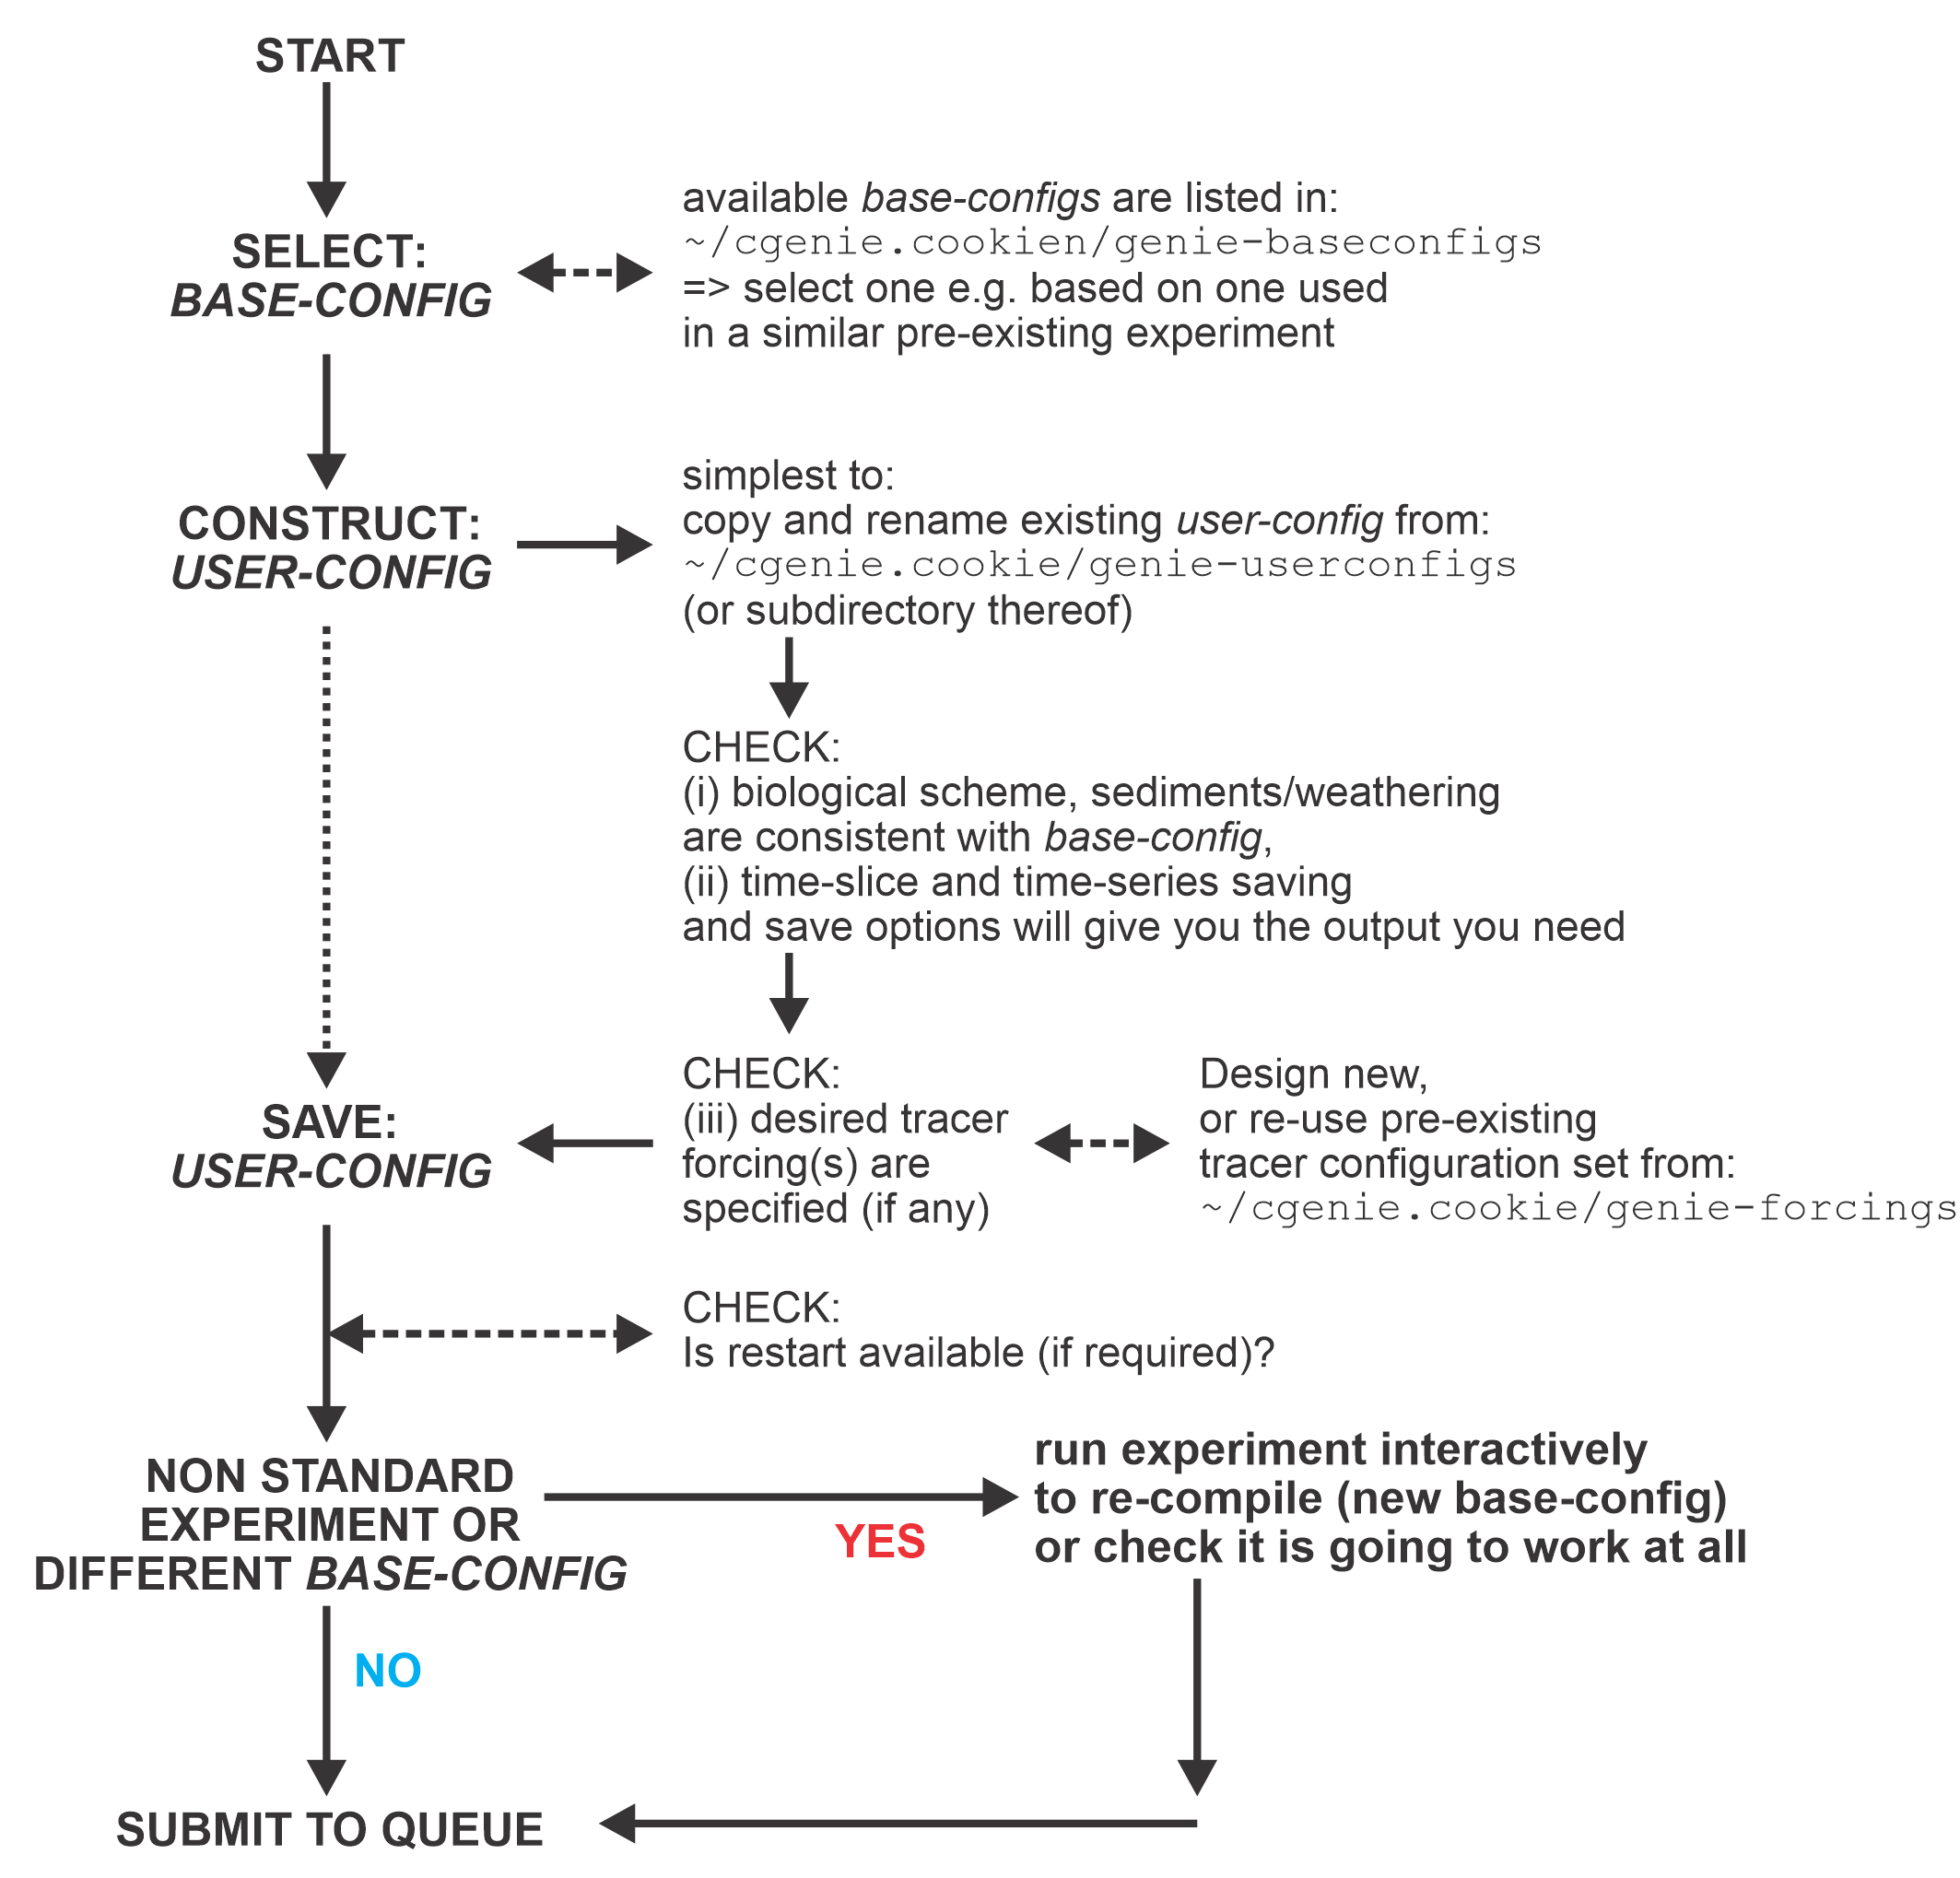
\includegraphics[width=0.9\textwidth]{Figures.usermanual.2.png}\centering
\vspace{2mm}
\caption{Schematic of the sequence-of-events in configuring and running an experiment.}
\label{fig:chx-jobcreation}
\end{figure}

%------------------------------------------------
\newpage
%------------------------------------------------

\section{Creating new experiments!}

The key to creating new experiments is to \textbf{remember that the name of the \textit{user-config} file, that contains the parameter settings that define that specific experiment, becomes the name of the experiment and hence name of the model results sub-directory in \textsf{\footnotesize cgenie\_output}}. Changing the name of the \textit{user-config} file, hence leads to a new experiment name and a new model results sub-directory. (Conversely, not changing the name of the  \textit{user-config} file and re-running it results in the results of any previous experiment run using that \textit{user-config} file, being over-written.)

%------------------------------------------------
\newpage
%------------------------------------------------

There are two obvious ways to create a new \textit{user-config} file and hence new experiment (although the simplest and recommended way, is the 2nd one):

\begin{enumerate}[noitemsep]

\vspace{1mm}
\item Create a blank text file \footnote{\texttt{\$ touch file.txt} will achieve this at the linux command line.} and populate the contents with the parameter value assignments you need for your new experiment.
\\Inevitably, it is difficult to remember all the names and even values you want to specify, meaning that you'll end up looking at existing \textit{user-config} files and copying and pasting lines (or even the entire contents) from the old file(s) into your new \textit{user-config} file. So then you may was well ...

\vspace{1mm}
\item Copy and edit an existing file!
\\This is the most practical approach -- pick an existing \textit{user-config} file that is closest to the specific experiment that you want to run -- copy and rename it, then edit the contents and save. For the purpose of trying this out, you can literally pick on any existing file in the \textsf{\footnotesize LABS } subdirectory (of \textsf{\footnotesize genie-userconfigs}).
\vspace{1mm}
\\ You can do this by:
\begin{itemize}[noitemsep]
\vspace{1mm}
\item Using your sftp client (program):
\\First -- drag the existing \textit{user-config} file to your local computer. On your local computer, rename the file as per how you would 'normally' rename any file. 
\\Now you can edit the parameter values, re-save it, drag it back to the cluster (from your local computer) using the sftp client ... and finally run the experiment.
\\There are also ways of configuring \textbf{sftp} clients so that you can double-click on a file in the remove window, edit it, and save it back to the remote computer.\footnote{Actually what happens is that the file is transferred locally, opened, and you edit a local copy. When you save it (locally), it is automatically transferred back.} 
\vspace{1mm}
\item Or, if you are comfortable working at the linux command line; working from the same directory (e.g. \textsf{\footnotesize LABS}) that the file you want to copy lives in, you can copy a file (to a new filename) by:
\\\texttt{\$ cp oldfile newfile }
\\(after which you can edit the new \textit{user-config} file \textsf{\footnotesize newfile}, re-save, and then run the experiment.)
\end{itemize}
\vspace{1mm}

\end{enumerate}

\noindent Remember that the new \textit{user-config} file needs to be saved in (or copied to) the \textsf{\footnotesize genie-userconfigs/LABS} sub-directory (in the case of experiments carried out as part of the tutorials described in this manual), or \textsf{\footnotesize LABS} itself or any sub-directory (or sub-sub- etc directory) ... as long as you specify the correct path to the directory where you save the new file to\footnote{See previous Section and the use of the 2nd parameter passed to \texttt{runcookie.sh}}.

%------------------------------------------------
\newpage
%------------------------------------------------

\section{Model output}

Experiment results are saved in a single sub-directory of the experiment results directory (along with a sub-directory for \textit{restart} files, and one for copies of your parameter choices). The experiment results directories all live in:

\vspace{-1mm}\begin{verbatim}
~/cgenie_output
\end{verbatim}\vspace{-1mm}
and will be assigned a directory name something like:

\vspace{-1mm}\begin{verbatim}
LAB.0.3.EXAMPLE
\end{verbatim}\vspace{-1mm}
(this being the results directory name for an experiment called \textsf{\footnotesize LAB.0.3.EXAMPLE}) and the actual results results hence in:

\vspace{-1mm}\begin{verbatim}
~/cgenie_output/LAB.0.3.EXAMPLE/results
\end{verbatim}\vspace{-1mm}

\noindent NOTE: If in an sftp client window you find that you cannot 'see' the \textsf{\footnotesize cgenie\_output} directory ... or cannot find any of the results sub-directories you are expecting, \uline{you will need to refresh the directory listing} (e.g. for \textbf{WinSCP}, there is a double green-arrow \textsf{\footnotesize Refresh} icon button near the top right of the window that you can click on). sftp client programs generally do not automatically refresh directory listing on the remote computer.

%------------------------------------------------
\vspace{1mm}\noindent\rule{4cm}{0.5pt}\vspace{2mm}
%------------------------------------------------

\noindent \textbf{cGENIE.cookie} has a flexible and powerful facility of saving results by means of spatially explicit ‘time-slices’, and as a semi-continuous ‘time-series’ of a single global (or otherwise representative mean) variable, described as follows.

%------------------------------------------------

\subsection{Time-slice output}

One of the most informative data sets that can be saved is that of the spatial distribution of properties (such as tracers or physical ocean attributes). However, saving full spatial distributions (e.g., a 36\(\times\)36\(\times\)8 array) for any or all of the tracers each and every time-step is clearly not practical; not only in terms of data storage but also because of the detrimental effect that repeated file access has on model run-time.
Instead, \textbf{BIOGEM} will save the full spatial distribution of tracer properties only at one or more predefined time points (in units of years). These are termed \textit{time-slices}. At the specified time points, a set of spatially-explicit data fields are saved for all the key tracer, flux, and physical characteristics of the system. However, rather than taking an instantaneous snapshot, the time-slice is constructed as an average over a specified integration interval (the default is set to 1.0 years, i.e. an annual average). \textbf{BIOGEM}  assumes that the specified time point represents the mid-point of the (annual) average with the results that output years end up being reported as e.g.,

\vspace{-1mm}\small\begin{verbatim}
0.5
1.5
2.5
4.5
…
\end{verbatim}\normalsize\vspace{-1mm}
(the mid-points of averages made over the intervals: 0-1, 1-2, 2-3, 4-5 years, etc.).

%------------------------------------------------
\newpage
%------------------------------------------------

\subsection{Time-series output}

The second data format for model output is much more closely spaced in time. Model characteristics must then be reducible to a single meaningful variable for this to be practical (i.e., saving the time-varying nature of 3-D ocean tracer distributions is not). Suitable reduced indicators would be the total inventories in the ocean and/or atmosphere of various tracers (or equivalently, the mean global concentrations / partial pressures, respectively). Like the time-slices, the data values saved in the time-series files represent averages over a specified integration interval (the default is set to 1.0 years (annual average) but the results are reported with respect to the mid-point of the average which is where the ‘.5’ bits come in again).

%------------------------------------------------

\subsection{File naming convention}

The \textsf{\footnotesize results} results directory will contain files with names of the form:

\vspace{1mm}
\begin{itemize}[noitemsep]
\setlength{\itemindent}{.2in}
\item \textsf{\footnotesize fields\_biogem\_2d.nc} – 2-D fields of ocean and atmosphere properties, as \textbf{NetCDF}.
\item \textsf{\footnotesize fields\_biogem\_3d.nc} – 3-D fields of ocean properties, as \textbf{NetCDF}.
\item \textsf{\footnotesize timeseries\_*.txt} – these are the time-series files (in ASCII / plain text format).
\item \textsf{\footnotesize SUMMARY\_AT\_year\_*\_diag\_GLOBAL.txt} – these contain (global diagnostics) summary information and are saved at the same frequency as the time-slices (also as ASCII / plain text).
\end{itemize}
\vspace{1mm}

%------------------------------------------------
\vspace{1mm}
\noindent\rule{4cm}{0.1mm}
%------------------------------------------------

\subsection*{Alternative file naming convention ...}

Having the e.g., 2D and 3D \textbf{netCDF} files always called the same name (\textsf{\footnotesize fields\_biogem\_2d.nc}, \textsf{\footnotesize fields\_biogem\_3d.nc}) in each and every experiment, has the potentil to get confusing if you have multiple experiments open simultaneously in a viewer such as \textbf{Panoply}.

You can specify that \textbf{netCDF} files are named following the name of your experiment, by adding the following line to your \textit{user-config}:

\vspace{-1mm}\begin{verbatim}
bg_ctrl_ncout_expid_name=.true.
\end{verbatim}

%------------------------------------------------
\newpage
%------------------------------------------------

\section{Viewing model output}

%------------------------------------------------

\subsection{Time-series output}

A descriptive summary of all the time-series (\textsf{\footnotesize biogem\_series\_*.res}) data files is given in the \textbf{cookie} User Manual if you are really that bored. The files of most immediate use/relevance are:

\vspace{1mm}
\begin{itemize}[noitemsep]
\setlength{\itemindent}{.2in}
\item \textsf{\footnotesize timeseries\_atm\_humidity.res}  - mean atmospheric (surface) humidity
\item \textsf{\footnotesize timeseries\_atm\_temp.res}      - mean atmospheric (surface) air temperature
\item \textsf{\footnotesize timeseries\_misc\_opsi.res}     - overturning stream-function (e.g. AMOC) strength
\item \textsf{\footnotesize timeseries\_misc\_seaice.res}   - mean ocean sea-ice cover and thickness
\item \textsf{\footnotesize timeseries\_ocn\_sal.res}       - mean ocean surface and whole ocean salinity
\item \textsf{\footnotesize timeseries\_ocn\_temp.res}      - mean ocean surface and whole ocean temperature
\end{itemize}

%------------------------------------------------
\vspace{1mm}\noindent\rule{4cm}{0.1mm}\vspace{2mm}
%------------------------------------------------

\noindent One way of viewing the contents of files (in a shell window/terminal) is to change directory to the experiment results directory and opening the file in a file editor at the command line. But that is not so much fun.

Instead – change to the experiment results directory and then to the \textsf{\footnotesize biogem} sub-directory in the Secure File Transfer Client, and try double-clicking (if you have set up the \textbf{WinSCP} preferences correctly) or right-mouse-button-clicking (the then Edit with) on one of the .res files (listed above).
\vspace{1mm}
For \texttt{timeseries\_ocn\_temp.txt}, you should see 5 columns:
\small\begin{verbatim}
 % time (yr) / temperature (C) / _surT (ice-free) (C) / _benT (C) / _surT (C)
\end{verbatim}\normalsize
for: model time (years) (actually, the mid-point in time of an annual average), annual mean ocean temperature (averaging over the entire ocean volume), annual mean ocean surface temperature (excluding ice-cover areas), annual mean benthic (sea-floor) temperature, annual mean ocean surface temperature (now including ice-cover areas). Other results files may differ in the numbers of columns but all should be identifiable from the header (first line) information.

Remember: \textbf{WinSCP} does not automatically refresh the directory listing. If you cannot see the results sub-directory with the experiment name you have just run, 99 times out of 100, it is because the display of the \textbf{WinSCP} needs to be refreshed -- there is an icon at the top of the program window or hit the ‘\textsf{\footnotesize F5}’ key.

\vspace{1mm}
\noindent\rule{4cm}{0.1mm}
\vspace{2mm}

\noindent For your information and edification (only): \textbf{Excel}, or \textbf{MUTLAB} if you prefer, can be used to graph the time-series results. Either way you will have to deal with the header line(s) that are present at the top of the file (and preceding the rows of data).

In \textbf{Excel}: Choose \textsf{\footnotesize File} then \textsf{\footnotesize Open}.  You will want to select \textsf{\footnotesize Files of Type} ‘\textsf{\footnotesize All Files (*.*)}’. In the \textsf{\footnotesize Text Import Wizard} window you can request that \textbf{Excel} skips the first few lines to start the import on the 2nd or 3rd line of the text file. Alternatively: set an appropriate column width manually in \textbf{Excel} to ensure that the columns of data are correctly imported.

\textbf{MUTLAB} will ignore lines starting with a \textsf{\footnotesize \%}, which the time-series starts with. However, it may be that the header line wraps-around and there is in effect a 2nd header line but without a \textsf{\footnotesize \%}. In this case, extra care (or a quick edit of the header in the ASCII file) will be required to load the data into \textbf{MUTLAB}.

%------------------------------------------------
\newpage
%------------------------------------------------

\subsection{2- and 3-D time-slice output}

For the time-slice \textbf{NetCDF} (*.nc) files you will be using a program called \textbf{Panoply}. If you want your own (FREE!) copy of this utility, you can get it here (and is available for: \textbf{Windoz}, \textbf{Mac}, and linux operating systems): http://www.giss.nasa.gov/tools/panoply/.

\vspace{1mm}

\noindent When you open the \textbf{NetCDF} file, you will be presented with a ‘\textsf{\footnotesize Datasets and Variables}’ window (on the left hand side of the application window). This contains a list of all the parameters available that you can display. You will find that the ‘\textsf{\footnotesize Long Name}’ description of the variable will be the most helpful to identify the one you want. Simply double-click on a variable to display. 

For the 3-D fields you will be asked first whether you want a ‘\textsf{\footnotesize \footnotesize Longitude-Latitude}’ or ‘\textsf{\footnotesize Latitude-Vertical}’ plot (for the 2-D fields, the plot display will immediately open).
For the ‘\textsf{\footnotesize Longitude-Latitude}’ plots – there are multiple levels (depth layers) in the ocean - these data that can be plotted from the surface to the abyssal ocean. For the ‘\textsf{\footnotesize Latitude-Vertical}' plots – there are multiple possible longitudes at which to plot slices. The default is the global mean meridional distribution. There is also an option for ‘\textsf{\footnotesize Longitude-Vertical}' plots (which we will not use).

There may be multiple time-slices (i.e., you can plot data saved from different years). By default, only the very first \textit{time-slice} will be displayed.

You can choose interpolate the data or not (often you may find that it is clearer not to interpolate the data but to leave it as ‘blocky’ colors corresponding to the resolution of the model), change the scale and colors, overlay continental outline, change the projection, etc etc. Grey cells represent ‘dry’ grid points, i.e., continental or oceanic crust.

\vspace{1mm}
NOTE: The default settings in \textbf{Panoply} can mislead. Be aware of:
\vspace{1mm}
\begin{enumerate}
\item \textbf{Panoply} initially displays the very 1st time-slice (often year mid-point 0.5) time-slice rather than the experiment end. This can confuse and look like an experiment has not done anything!
\item By interpolating the data (not always misleading). To remove interpolation, un-tick:
\\‘\textsf{\footnotesize Interpolate}’ in the ‘\textsf{\footnotesize Arrays}’ tab.
\item By displaying a global zonal mean by default when selecting \textsf{\footnotesize Latitude-Vertical} plots. Then, to further confuse you, by plotting the output up-side-down (to invert: in the ‘\textsf{\footnotesize Grid}’ tab, hit ‘\textsf{\footnotesize Swap B/T}’ (for swap bottom/top).
\item By listing all ‘\textsf{\footnotesize Plottable variables}’ (option at the bottom of the window), when what you \textit{ideally} want are  the shorter and less confusing list of ‘\textsf{\footnotesize Georeferenced variables}’.
\item In \textsf{\footnotesize Longitude-Latitude} plots, by overlaying the modern continental output. (\textbf{cookie} land is marked in grey.)
\item By fitting a scale to the plot when the display window is opened, but not changing the scale when e.g., time or depth is changed. (The point of confusion is that you can quickly move outside the scale and end up with all model points dark blue or red.) Re-fit the scale, or manually set limited, in the ‘\textsf{\footnotesize Scale}’ tab.
So be careful when opening a new plot that you are looking at what you *think* you are looking at …
All the defaults can be changed via the ‘\textsf{\footnotesize Edit}’ drop-down menu and ‘\textsf{\footnotesize Preferences}’.
\end{enumerate}

%------------------------------------------------
\vspace{1mm}\noindent\rule{4cm}{0.1mm}\vspace{2mm}
%------------------------------------------------

\noindent To save plots in \textbf{Panoply}:
\footnotesize
\\\textsf{File}
\\\textsf{Save Image As …}
\normalsize
\\Then select the location, filename, and graphics format.

%------------------------------------------------
\newpage
%------------------------------------------------

\section{Submitting experiment ‘jobs’}

This bit is no particular fun at all, but it is a very handy ‘trick’ for running the model in the background, and maximizes drinking time in the bar vs. sat bored watching a computer screen :)

%------------------------------------------------
\vspace{1mm}\noindent\rule{4cm}{0.1mm}\vspace{2mm}
%------------------------------------------------

\noindent Running jobs interactively is all very well, but there are three important limitations:
\begin{enumerate}[noitemsep]
\vspace{1mm}
\item The connection between your terminal and the server computer running the model must remain unbroken. Anything more than a fleeting loss of internet connectively may result in the experiment terminating.
\vspace{1mm}
\item You can only run one experiment at a time … unless you want to have thousands of separate terminal open …? I thought not …
\vspace{1mm}
\item Any cluster or computer you are likely to be accessing using a shell will not have many computing cores itself, either because it is a single machine with only one or two processors, or if a cluster, by using a terminal you are running on the ‘head node’, which will have similar computing core limitations to running on a single machine. The more experiments you run simultaneously, the slower they will all run …
\end{enumerate}

%------------------------------------------------
\vspace{1mm}\noindent\rule{4cm}{0.1mm}\vspace{2mm}
%------------------------------------------------

\noindent The alternative is to submit your experiment as a ‘job’ to a queuing system which then manages what compute resources are used to run the model. Once you have submitted the experiment, that is it – you can go straight to the bar :)

For example -- to run the same experiment as before (\textsf{\footnotesize LAB\_0.EXAMPLE}) for maybe 100 years (or even longer if you wish – I am just pulling factors of 10 out of thin air here) but now submit the experiment as a job to the cluster queue, type (again: SINGLE, CONTINUOUS LINE):
\vspace{-1mm}
\small\begin{verbatim}
$ qsub -q QUEUE.q -j y -o cgenie_log -V -S /bin/bash runcookie.sh
  ./runcookie.sh cookie.CB.p_worbe2.BASES LABS LAB.0.3.EXAMPLE 100
\end{verbatim}\normalsize
\vspace{-1mm}

Here, the queue name for this\ particular cluster is \textsf{\footnotesize QUEUE.q}. \uline{The cluster you are actually using will have a different queue name} (e.g. refer to any cluster-specific information that you might have).

\vspace{1mm}
Note that now you should omit the ‘\texttt{./}’ bit before \texttt{runcookie.sh}.
(If you are interested (I know that you are not): the options following \texttt{qsub} and before \texttt{runcookie.sh} do things like re-directing screen output and error messaging to a file and specify which linux ‘shell’ to assume. It is even possible to receive an email when the job is done :) )
The status of the cluster queue and how you experiment job is getting on (e.g., “Is it finished yet?”) can be checked by typing:
\vspace{-1mm}
\small\begin{verbatim}
$ qstat -f
\end{verbatim}\normalsize
\vspace{-1mm}
(\texttt{qstat -f -u "*"} will show all jobs on the cluster.)

\vspace{1mm}
After submitting an experiment, you receive a job number. This number appears in the first column in the queue status information when you issue a qstat –f command. You should see your job appear on one of a number of compute nodes, perhaps numbered 0-0 through 0-5), although it might briefly reside as a ‘\textsf{\footnotesize PENDING JOB}’. For each node, there are multiple processing cores (depending on the specific cluster and queue), meaning that multiple instances of \textbf{cookie} can run simultaneously on each node. For an 8-level ocean based configuration of \textbf{cookie}, being run for 100 years, the job should remain there in the queue for a few minutes before ‘disappearing’ (your clue that it has finished, or died\footnote{If your experiment appears on the queue but vanishes after a few seconds, it has most likely died :(} …). If you periodically re-issue a \texttt{qstat –f} command you can follow your job’s progress.

A rough rule of thumb is that 8-level ocean \textbf{cookie} @ a horizontal grid resolution of 36x36 will simulate about 1000 years per CPU hour. The 16-level version (which you will use later), runs at about 300-400 years per CPU hour.

\vspace{1mm}
\noindent \textbf{NOTE}: It may be that the \textbf{FORTRAN} compiler is not accessible by the computer nodes. The implication of this is that \textit{the \textbf{cookie} executable must be already compiled BEFORE a job is submitted to the queue}. In other words; if you have just changed the model resolution or continental configuration, or number of tracers (i.e. changed the \textit{base-config}) or issued a \texttt{make cleanall} command you MUST briefly run your desired experiment (or equivalent) interactively (i.e., in the shell window) to ensure that everything is correctly compiled. For instance, either run the experiment for a couple of years or start the experiment for the desired full duration, but 'kill it' (\textsf{\small Ctrl-C}) once the experiment is running successfully.

%------------------------------------------------
\newpage
%------------------------------------------------

\section{‘Restarts’}

Not much fun here either … but again... an important and time-saving (== increased drinking time!) modelling technique to learn to use.

By default, model experiments start from ‘cold’, i.e., the ocean is at rest and uniform in temperature and salinity while the atmosphere is uniform in temperature and humidity. All biogeochemical tracers in the ocean have uniform concentrations and/or are zero and there are no biogenic materials in deep-sea sediments. From this state it will take several thousand years (kyr) for the climate system to reach steady-state, and closer to 5 kyr (or more) for ocean biogeochemical cycles and atmosphere \(CO_{2}\) to reach steady-state, and exceeding 100 kyr for sediment composition to re-balance weathering ... Reaching this the equilibrium state is called the ‘\textit{spin-up}’ phase of the model.
There is evidently little point in repeating the \textit{spin-up} for each and every model experiment that are similar except in a single detail (e.g., testing a variety of different \(CO_{2}\) emissions scenarios all starting from current year 2012 conditions). A facility is thus provided for requesting that a ‘\textit{re-start}’ is used – starting a new experiment from the end of a previous one, usually a \textit{spin-up} that has been run explicitly for the purpose of generating a starting point (\textit{re-start}) of the system at steady-state (equilibrium) for subsequent experiments to continue on from.
It is important to note that there is nothing special about a \textit{re-start} – it is simply an experiment that you have already run. Equally, there is nothing special about the \textit{re-start}s you will download next – these you could have generated yourself – it simply saves time to have them provided.

\vspace{1mm}
\noindent\rule{4cm}{0.1mm}
\vspace{2mm}

\noindent To experiment with using a \textit{re-start}, you will first need to download a file that has been created (a pre-run 10,000 year spin-up). To fetch this: Change to the \textsf{\footnotesize cgenie\_output} directory (perhaps by going ‘home’ first (\texttt{cd} \textsf{\small <Enter>}), and then changing to \textsf{\footnotesize cgenie\_output} – refer to linux commands HOW-TO and Figure 1.1), and type:

\vspace{-2mm}\small
\begin{verbatim}
$ wget --no-check-certificate http://www.seao2.info/cgenie_output/
   cookie.CB.p_worbe2.BASES.ridgwelletal.SPIN.tar.gz
\end{verbatim}\normalsize
\vspace{-2mm}
(all one line!)

This downloads an archived/compressed copy of the restart from a location on the interweb. Extract the contents of this archive by typing:

\vspace{-2mm}\small
\begin{verbatim}
$ tar xfzv cookie.CB.p_worbe2.BASES.ridgwelletal.SPIN.tar.gz
\end{verbatim}\normalsize
\vspace{-2mm}

Finally, change directory back to \textsf{\footnotesize cgenie.cookie} and then \textsf{\footnotesize genie-main} so that you are ready to run the model (the model is *always* run from the \textsf{\footnotesize cgenie.cookie/genie-main} directory).

\vspace{1mm}
\noindent\rule{4cm}{0.1mm}
\vspace{2mm}

\noindent A \textit{re-start} can be requested for  running on a new experiment from the end of a previous one, by providing a 5th (optional) parameter when entering in the \texttt{runcookie.sh} command. A spin-up of the modern World climate state is provided for you as a \textit{restart} -- 
\textsf{\footnotesize cookie.CB.p\_worbe2.BASES.ridgwelletal.SPIN} -- which you have just unpacked to the \textsf{\footnotesize cgenie\_output} results output directory.

To test out the use this \textit{restart} -- create a new (\textit{user-config}) experiment configuration file in the directory: 

\vspace{1mm}
\textsf{\footnotesize \(\sim\)/cgenie.cookie/genie-userconfigs/LABS}
\vspace{1mm}

\noindent taking the file \textsf{\footnotesize LAB\_0.3.EXAMPLE} (which is provided) as a template (no parameter changes need to be made yet). As described earlier -- copy this file and give it a new name -- here, name it: \textsf{\footnotesize LAB.0.3.NEW}

%------------------------------------------------
\newpage
%------------------------------------------------

\noindent You can then specify the use of the \textit{restart} in your new \textsf{\footnotesize LAB\_0.3.NEW} experiment:

\vspace{-2mm}
\small\begin{verbatim}
$ ./runcookie.sh cookie.CB.p_worbe2.BASES LABS LAB.0.3.NEW 100 
   cookie.CB.p_worbe2.BASES.ridgwelletal.SPIN
\end{verbatim}\normalsize
\vspace{-2mm}

The run-time output should now look noticeably different. There should be no (or perhaps just very little) drift in any of the various variable values outputted to the screen – this is because you have (re-)started from the end of a run that had already ready an equilibrium (or close).

Because \textsf{\footnotesize LAB.0.3.EXAMPLE} (and hence your copy, \textsf{\footnotesize LAB\_0.3.NEW}) does not prescribe a value of $pCO_2$ but instead allows it to 'float', your experiment is a good test of whether the carbon cycle in experiment \\\textsf{\footnotesize cookie.CB.p\_worbe2.BASES.ridgwelletal.SPIN} was at steady state.

%----------------------------------------------------------------------------------------
%----------------------------------------------------------------------------------------
%%----------------------------------------------------------------------------------------
%       CHAPTER 01
%----------------------------------------------------------------------------------------

\cleardoublepage

\chapterimage{Figure-1-The-image-of-an-ice-encased-Earth-a-Snowball-Earth-with-oases-of-open-water-on.png} % Chapter heading image

\chapter{Climate Dynamics \& Experimental Design}\label{ch:climate-dynamics}

\hfill \break

%------------------------------------------------
\newpage
%------------------------------------------------

\section{(none)}

%----------------------------------------------------------------------------------------
%----------------------------------------------------------------------------------------
%----------------------------------------------------------------------------------------
%       CHAPTER 01
%----------------------------------------------------------------------------------------

\cleardoublepage

\chapterimage{Figure-1-The-image-of-an-ice-encased-Earth-a-Snowball-Earth-with-oases-of-open-water-on.png} % Chapter heading image

\chapter{Climate dynamics \& experimental design}\label{ch:climate-dynamics}

\hfill \break

\noindent Stuff to keep in mind:

\vspace{2mm}
\begin{itemize}
\item Models ARE NOT the ‘real World’ (it is going to be pretty obvious this is the case here).
\item Don’t believe what you read in \textit{Nature} or \textit{Science} ...
\end{itemize}

%------------------------------------------------
\newpage
%------------------------------------------------

\section*{Readme}

You will need to download a new \textit{restart} file prior to embarking on the snowball Earth experiments.
To fetch this: change directory to the \textsf{\footnotesize cgenie\_output} directory, and type (or copy and paste carefully from this PDF ...):
\vspace{-2mm}
\small\begin{verbatim}
$ wget --no-check-certificate http://www.seao2.info/cgenie_output/
   cookie.C.p_woreq1.NONE.SPIN.tar.gz
\end{verbatim}\normalsize
\vspace{-2mm}
(All one line, but note that there is no space after '\texttt{cgenie\_output/}' and before
\\'\texttt{cookie.C.p\_woreq1.NONE.SPIN.tar.gz}'.)

\vspace{1mm}
This downloads an archived/compressed copy of the experiment \textsf{\footnotesize cookie.C.p\_woreq1.NONE.SPIN} – effectively, just an experiment (spin-up) that has already been run for 5,000 years for you. Extract the contents of this archive by typing (also from the \textsf{\footnotesize cgenie\_output} directory):
\vspace{-2mm}
\small\begin{verbatim}
$ tar xfzv cookie.C.p_woreq1.NONE.SPIN.tar.gz
\end{verbatim}\normalsize
\vspace{-2mm}

A new experiment results directly will then appear as if you had just run the entire 10,000 year experiment yourself (and you could in fact have done so). Remember to refresh the \textbf{WinSCP} directory view window if you are using this particular software, or it might appear that nothing has been extracted.

\vspace{1mm}
You’ll then need to change directory back to \textsf{\footnotesize genie-main} to run the model.

\vspace{1mm}
If ... when you subsequently try and use this \textit{restart} in an experiment, \textbf{cookie} stops and complains that it cannot find it, check:
\begin{enumerate}[noitemsep]
\item That you in fact downloaded it to the correct directory, which should be: \textsf{\footnotesize cgenie\_output}, and not randomly to e.g. your home directory ...
\item That you unpacked it.
\end{enumerate}

%------------------------------------------------
\newpage
%------------------------------------------------

\section{Brrrrrrrrrrrr – it’s chilly on ... snowball Earth!}

To illustrate how ‘easy’ it can be to configure an Earth system / climate model such as \textbf{cookie} and explore the behavior of the Earth system and its response to perturbation – you are going to induce an extreme cooling of the climate system and see what happens. 

Solar output was weaker during the late Neoproterozoic, a time when the Earth experienced a series (2 ish) of extreme glaciations. Thus, having a mild climate state to start with must have been dependent on sufficient \(CO_{2}\) and/or \(CH_{4}\) in the atmosphere which presumably must have been highly elevated compared to the modern World ... sort of opposite to the problem we have today …

%------------------------------------------------
\vspace{1mm}
\noindent\rule{4cm}{0.5pt}
\vspace{2mm}
%------------------------------------------------

\noindent You are going to be running experiments in a similar manner to before, and using the \textit{re-start} experiment that you downloaded. You could then, for example, take the experiment configuration file \textsf{\footnotesize LAB.1.1.EXAMPLE} (which is provided for you), and run the experiment, which has a new \textit{base-config}: \textsf{\footnotesize cookie.C.p\_woreq1.NONE}, by typing:
\vspace{-1mm}
\small\begin{verbatim}
$ ./runcookie.sh cookie.C.p_woreq1.NONE LABS LAB.1.1.EXAMPLE 100 
   cookie.C.p_woreq1.NONE.SPIN
\end{verbatim}\normalsize
(All one line ... but remember there will need to be a space separating the experiment duration and the name of the \textit{restart}).

\noindent \uline{However} ... why not get into the habit of creating new and uniquely named experiments and their associated \textit{user-config} files (no harder than copying it and renaming it -- see earlier). If you keep using the same experiment name, the results will be over-written each time you re-run that experiment, whilst having  2 (or more) experiments running simultaneously with exactly the same name causes havoc as they try and over-write each others results files in a somewhat entertaining but ultimately useless way. 

\vspace{1mm}
So -- copy and rename the file \textsf{\footnotesize LAB.1.1.EXAMPLE} to ... \textsf{\footnotesize LAB.1.1.EXPT} or whatever (in the subdirectory \textsf{\footnotesize LABS}), and then run your newly created experiment:
\vspace{-1mm}
\small\begin{verbatim}
$ ./runcookie.sh cookie.C.p_woreq1.NONE LABS LAB.1.1.EXPT 100 
   cookie.C.p_woreq1.NONE.SPIN
\end{verbatim}\normalsize

Remember that because you have changed \textit{base-config} since the exercises in the previous chapter, running the model first interactively (at the command line) is essential in order for the model code to be re-compiled consistent with the new configuration. i.e. you cannot directly start submitting experiments using the \textit{base-config} \textsf{\footnotesize cookie.C.p\_woreq1.NONE}, straight-away after having previous run the model using the \textsf{\footnotesize cookie.CB.p\_worbe2.BASES} \textit{base-config}. Once you have re-compiled the model with the new \textit{base-config} and starting running (any experiment), you need not re-compile again and can submit as many jobs to the cluster queue as you like, up until you change \textit{base-config} once again.

%------------------------------------------------
\vspace{-1mm}
\noindent\rule{4cm}{0.5pt}
\vspace{2mm}
%------------------------------------------------

\noindent Overall: your task in this exercise will be to determine the radiative forcing (or rather, p\(CO_{2}\) equivalent) threshold required to drive the climate system into a full ice-covered ocean (snowball Earth) state. (Make sure you have read the \textit{Hyde et al.} [2000] paper.)

Useful 2-D (netCDF —- \textbf{Panoply}) variables to view include: surface air temperature and sea-ice extent (and/or thickness). Ocean surface temperature and salinity can be viewed in the 3-D netCDF results file but are likely to be of less interest.

Time-series (ASCII \textsf{\footnotesize .res} files) are useful for providing simple mean indicators of global climate such as global ocean fractional sea-ice covered.

Note that the model configuration of an idealized super-continent you are using and as defined by the \textsf{\footnotesize cookie.C.p\_woreq1.NONE} \textit{base-config} file, positioned symmetrically about the Equator, is pretty unrealistic. But the further you go back in time, the more uncertain it becomes as to exactly where and in what orientation the continents were. Sometimes modelers have to resort to somewhat idealized experiments if the uncertainties are too great. In addition, one can conduct sensitivity experiments to test whether the continental configuration is important to the results. For instance, \textit{Hoffman and Schrag} [2002] discuss the potential importance of continental configuration, while the hypothesis of \textit{Donnadieu et al.} [2004] rests on specific details of the continental configuration.

For this configuration, the solar constant is set weaker than modern to reflect the fact that the Sun’s output has increased with time and during the Neoproterozoic the solar constant would have been ca. 5\% weaker. This is set in the \textit{user-config} file by the model \textit{parameter}:

\vspace{-1mm}
\small\begin{verbatim}
ma_genie_solar_constant= 1285.92
\end{verbatim}\normalsize
\vspace{-1mm}

\noindent which is set at the top of the provided \textit{user-config} file \textsf{\footnotesize LAB.1.1.EXAMPLE}. (For reference, the modern value is \( 1368 Wm^{-2}\).)

%------------------------------------------------
\vspace{1mm}
\noindent\rule{4cm}{0.5pt}
\vspace{2mm}
%------------------------------------------------

\noindent To search for the atmospheric \(CO_{2}\) concentration (or rather, radiative forcing equivalent) that would lead to a ‘snowball Earth’ state in the Neoproterozoic and answer the question:
‘How low does \(CO_{2}\) have to be to trigger a ‘snowball’?’
you are going to edit the experiment file that controls the specific details of the experiment -- the \textit{user-config} file. From the \textsf{\footnotesize genie-userconfigs/LABS} directory, open one of the snowball experiments in your preferred  text editor. 

Near the top of the file you should see something like:

\vspace{-2mm}
\small\begin{verbatim}
#
# --- CLIMATE ---------------------------------------------------------
#
…
# scaling for atmospheric CO2 radiative forcing, relative to 278 ppm
ea_radfor_scl_co2=20.0
…
\end{verbatim}\normalsize
\vspace{-1mm}

Each line that is not commented out (i.e., no \#) contains a \textit{parameter} name and assigned value pair, with the format:
\vspace{-1mm}
\small\begin{verbatim}
PARAMETER=VALUE
\end{verbatim}\normalsize
\vspace{-1mm}
The value of each parameter can be edited to change the experiment. (Additional parameter value specifications can also be added, or existing ones deleted.) In this example, the line:
\vspace{-1mm}
\small\begin{verbatim}
ea_radfor_scl_co2=20.0
\end{verbatim}\normalsize
\vspace{-1mm}
specifies a radiative forcing of climate by \(CO_{2}\) equivalent to x20 modern (20x278 = 2560 ppm). If you instead wrote:
\vspace{-1mm}
\small\begin{verbatim}
ea_radfor_scl_co2=1.0
\end{verbatim}\normalsize
\vspace{-1mm}
this would give you a modern\footnote{Technically: the pre-industrial \(CO_{2}\) value rather than ‘modern’ \textit{per se.}} (x1, or 1x278 = 278 ppm) radiative forcing.
Note: \(CO_{2}\) is not being explicitly modeled in this experiment\footnote{And hence the parameter:
\\\texttt{\# set no CO2 climate feedback}
\\\texttt{ea\_36=n}
\\which tell cookie to ignore the concentration of CO2 in the atmosphere, in case, as here, there isn't one defined ...}, but the long-wave radiative forcing associated with a specified concentration of \(CO_{2}\) (in ratio to modern) is being set instead.

Edit the value of \texttt{ea\_radfor\_scl\_co2} (lower or higher -- your choice) and save the file (\uline{with a different filename!}). Re-run the experiment until sea-ice extent starts to approach a new steady state. You may want to try  longer simulations than suggested (\textgreater 100 years) if it becomes clear that the model is still far from steady-state by the end of the experiment. You can judge how close to equilibrium things have got by following (and/or plotting) the evolution of e.g., global surface air temperature or sea-ice extent (both time-series files).

%------------------------------------------------
\vspace{1mm}
\noindent\rule{4cm}{0.5pt}
\vspace{2mm}
%------------------------------------------------

\noindent 
In terms of methodology -- or; 'how am I going to answer the question' -- you will need to run mutilple different model experiments, each with a different value for the radiative forcing parameter, and find out for what value of the parameter, the Earth becomes completely ice-covered. It is your choice whether you change the radiative forcing parameter value, run the experiment, but wait for it to finish before deciding the radiative forcing parameter value to try for the next experiment -- i.e. a sequential approach, or try running multiple different 'guesses' simultaneously by submitting multiple different experiments to the queue. Ideally, each experiment will have a different name.

In each experiment, you want to be assessing how far towards the Equator the sea-ice limit encroaches by viewing some of the \textit{time-series} and \textit{time-slice} files or even the on-screen summary feedback (assuming that you are running interactively rather than via a job submission to the cluster queue). Informative \textit{time-series} variables include (but are not necessarily be limited to): atmospheric temperature and sea-ice cover. (Sea-ice thickness, on account of the simple physics in the model, low resolution and long time-step, can fluctuate a little. This is also true for sea-ice area. Sea-ice volume is then the most reliable data (column) to keep track of in the \textit{time-series} output.)

For the \textit{time-slice} data: atmospheric and ocean surface temperature and particularly sea-ice extent (fractional cover), (2-D biogem \textbf{NetCDF} file) may be informative.

HINT: Be careful with the ‘\textsf{\footnotesize Fit to data}’ scaling feature in \textbf{Panoply} – at near complete sea-ice cover, you may find Panoply scaling min and max sea-ice between 99.1 and 99.9\% or something. Specific fixed scale limits (e.g. 0 and 100) can be set instead.

In answering the question (‘How low does \(CO_{2}\) have to be to trigger a ‘snowball’?’), think about what an appropriate degree of precision (rather than accuracy) might be for your experiments. Just because computer models generally calculate to around 16 significant places of precision, does not mean you have 16 significant figures of realism. For instance – how many significant figures is the solar constant quoted to and what do you think is the uncertainty in this? Harder to judge is how the assumed (incorrect) continental configuration creates additional uncertainty, or the simple physics assumed in the ocean or sea-ice, or lack of snow on land …

\vspace{1mm}
Other questions to think about with regards to numerical modeling are:

\begin{itemize}[noitemsep]
\setlength{\itemindent}{.2in}
\vspace{1mm}
\item  (Is the model configuration and experimental design ‘realistic’ ... ?)
\vspace{1mm}
\item  What is ‘missing’ in the model and what might the implications for your predictions and conclusions be? For example, there is no land-surface scheme (and hence no concept of ‘snow’) in this particular configuration.
\vspace{1mm}
\item Are the simulations being run for sufficiently long? Why not if not (i.e., justify your choices of parameter values and experimental assumptions)? How might the results and conclusions be biased (if at all)?
\vspace{1mm}
\item How would you test model predictions and your overall conclusions?
\vspace{1mm}
\item How could the experimental design be improved?
\end{itemize}

\vspace{1mm}
\noindent Associated with the question of 'precision' is: '\textit{How long do I have to run the experiment for?}'

This also has a vague-to-no answer. It depends on the science question and what you might judge to be appropriate precision in the context of the various uncertainties ... In other words -- if you can define a sufficient or minimum precision of some property of the system, you only need to run the model as long as needed to achieve this. However, to determine  the precision of the model at any point in time, you need to know the final or equilibrium value. So ideally you would run the model once, for much longer than you think you need to, and then determine how as a function of time, precision increases and error between current state and final steady state decreases.

Here I am crudely equating the concept precision with how far the model is from steady-state. You could think about is in terms of accuracy if you assumed that the steady-state of the model was 'perfect' and deviations from that steady-state (i.e. incomplete spin-up) equates to model 'error'.

%------------------------------------------------
\vspace{1mm}
\noindent\rule{4cm}{0.5pt}
\vspace{2mm}
%------------------------------------------------

\noindent Once you are happy  with determining snowball threshold, try and answer the associated question:

\vspace{2mm}
\noindent \textit{How high does the (\(CO_{2}\)) radiative forcing have to be in order to \uline{escape} from a snowball?}
\vspace{2mm}

\noindent Having determined the appropriate radiative forcing value required to create a snowball state, you can use that particular experiment as a \textit{re-start}, and hence carry out a series of experiments with increasing radiative forcing, all starting from the same within-snowball climate state you have just created. Defining the radiative forcing / climate path going out of a snowball would complete the hysteresis loop of \textit{Hyde et al.} [2000]. 

Note that a good \textit{re-start} is one for which the experiment did not sit too long in the snowball state before finishing (the more sea-ice thickness you create in the first experiment, the more you are going to have to melt in the next and hence the longer this new series of experiments will take to ruin…). To achieve this, you can fine-tune the number of years the experiment is run, i.e. having determined the appropriate radiative forcing value required to create a snowball state, find out when (in terms of number of years) in the experiment the snowball state first occurred, and then run a new experiment that finishes only a decade or so after the snowball state was initiated.\footnote{You cannot select when the \textit{re-start} is saved – it is always saved at the end of an experiment.}

HINT: If you are having trouble deciding whether or not the snowball is heading in the right direction (i.e. towards an exit!), e.g. because sea-ice is always reported at 100\% (or close to), you can keep track of whether there is net melting or net freezing by following mean sea-ice thickness (m) as reported in the \textsf{\footnotesize biogem\_series\_misc\_seaice.res} time-series output file. Your indication of a melting snowball state is a progressive decline in mean thickness (a proxy for global ice volume). \uline{Note that you can open and review the results of \textit{time-series} files at *any* time during the experiment as the lines are written while the data for each time point is generated.}

Overall: think critically about the model configuration, the experimental design, and the nature of the scientific question (based on your background reading of snowball Earth). Some of the exploration/testing suggestions (above) may not necessarily give substantially different results. Such a finding would be as valid and interesting as determining an important dependence of a certain assumption, and would for instance indicate that the associated paleo uncertainties are not critical to model assessment of the question.

Always be prepared to justify all your choices for experimental design and model settings, e.g., range of radiative forcing assessed, continental configuration(s), solar forcing, use of re-starts (if any), run duration, etc. etc. etc. etc.

%------------------------------------------------
\newpage
%------------------------------------------------

\section{Further ideas}

%------------------------------------------------

\subsection{Feedback loop analysis}

To quantify the snowball Earth hysteresis loop in \textbf{cookie} as per Figure 2 in \textit{Hyde et al.} [2000] you will need to extract from the model ‘meaningful’ measures of climate (e.g., global surface air temperature, fractional sea-ice coverage) as a function of \(CO_{2}\) multiples, \(CO_{2}\) concentration, or (better) radiative forcing. For the latter, in \textbf{cookie}, the radiative forcing for a doubling of \(CO_{2}\) is set at: \(5.77 Wm^{-2}\). See: \textit{Myhre et al.} [1998] (Geophys. Res. Lett. 25, 2715–2718) and/or \textit{IPCC} [2007] for more on what radiative forcing is and how it is related to a relative change in \(CO_{2}\) concentration. Also, for making a comparison with \textit{Hyde et al.} [2000] -- for going into the snowball, note that they plot the change in radiative with a ‘cooling’ as positive (a bit daft). Their baseline radiative forcing state (an anomaly of \(0 Wm^{-2}\)) you might assume is equivalent to 278 ppm and hence \(\backsim\)130 ppm is an approximately halving of \(CO_{2}\) and hence creates \(\backsim5 Wm^{-2}\) of cooling. (You might prefer to plot the radiative forcing change as warming being positive, which makes rather more sense ...)

For coming out of a snowball, because the \(CO_{2}\) and hence radiative forcing threshold is so high as compared to going in, you may want to be creative in the plotting (assuming attempting to combine both thresholds into a single plot) and, for instance, one might break the scale between the low radiative forcing interval spanning going in and the high one spanning coming out.

Another example is as per Figures 3 and 4 in \textit{Stone and Yao} [2004] (Clim. Dyn. 22, 815–822) (although here it is the solar constant rather than long-wave radiation forcing that is being varied). So in fact, you could try varying the solar constant as an alternative to radiative forcing and hence be able to come up with a plot directly comparable to \textit{Stone and Yao} [2004].

%------------------------------------------------

\subsection{Continental configuration (1)}

It was mentioned earlier that the position of the continents is an area of modeling uncertainty and might be important. You can test for this. Four alternative \textit{base-configs} are provided, each defining a different continental configuration:

\vspace{1mm}
\begin{enumerate}[noitemsep]
\setlength{\itemindent}{.2in}
\item
\begin{verbatim}
cookie.C.p_worpl1.NONE
\end{verbatim}
 – a single polar super-continent, with an ocean resolution of 36x36 with 8 vertical levels. (Note potential ‘l’ and 1’1 confusion in ‘\textsf{\footnotesize p\_worpl1}’.)
\item
\begin{verbatim}
cookie.C.p_worpl2.NONE
\end{verbatim}
  – one continent at each pole, with an ocean resolution of 36x36 with 8 vertical levels.
\item
\begin{verbatim}
cookie.C.p_woreq1.NONE
\end{verbatim}
  – a single Equatorially-centred super-continent, with an ocean resolution of 36x36 with 8 vertical levels. [this is the current configuration (that you  used previously)]
\item
\begin{verbatim}
cookie.C.p_woreq2.NONE
\end{verbatim}
 – two continents straddling the Equator, with an ocean resolution of 36x36 with 8 vertical levels.
\end{enumerate}
\vspace{1mm}

You can use the given \textit{user-config} file (\textsf{\footnotesize LAB.1.1.EXAMPLE}) again as an experiment template file, and any of the alternative configurations can be run very similarly to as per before, i.e.:

\vspace{-2mm}
\begin{verbatim}
$ ./runcookie.sh cookie.C.p_xxxxxx.NONE LABS LAB.1.1.EXAMPLE 100
\end{verbatim}
\vspace{-2mm}

Note that you are using a different \textit{base-config} file name: \textsf{\footnotesize cookie.C.p\_xxxxxx.NONE}
\\where \textsf{\footnotesize xxxxx} is one of: \textsf{\footnotesize worpl1}, \textsf{\footnotesize worpl2}, \textsf{\footnotesize woreq1}, or \textsf{\footnotesize woreq2}.

\uline{Also note} that \uline{no} \textit{re-starts} are provided for any of these configurations. You may (or may not) want to create some (you will need to judge for yourselves how long to run the \textit{re-start} experiments to achieve as close to steady-state as you think is ‘sufficient’). Recall again, that \textit{re-starts} are just ‘normal’ experiments that have already been run.
Be careful that when changing from one \textit{base-config} to another, the model re-compiles. Simply running the new configuration briefly (for even just a single year) is sufficient to ensure this. Experiments can then be safely submitted to a cluster queue, i.e. do not try and submit an experiment using a different \textit{base-config} straight to the cluster queue without having run it (or a short version of the experiment you want) interactively first (to ensure the model is re-compiled). This is also good practice – checking that a new sort of experiment and/or model configuration works as you intend and without hiccups.

%------------------------------------------------

\subsection{Continental configuration (2)}

Although much useful can be learned from conceptual configurations and Worlds regarding climate dynamics, it is invariably aesthetically more 'pleasing' to also test ideas in a more paleogeographically realistic configuration. Provided is a set of \textit{base-config} and \textit{user-config} files (plus associated boundary conditions) for the position of the continents and climate 635 millions years ago (635 Ma). For this:

\vspace{1mm}
The \textit{base-config} is named: \textsf{\footnotesize cookie.C.fm0635cb.NONE}

\vspace{1mm}
The \textit{user-config} is: \textsf{\footnotesize cookie.C.fm0635cb.NONE.SPIN}

\vspace{1mm}
NOTE that the \textit{user-config} lives in the directory: \textsf{\footnotesize \(\sim\) \textbackslash cgenie.cookie\textbackslash user-configs\textbackslash EXAMPLES}

\noindent so that you either need to specify this different (\textsf{\footnotesize EXAMPLES}) directory when running \textbf{cookie}, or copy the \textit{user-config} file into \textsf{\footnotesize LABS}.

\vspace{1mm}
A \textit{re-start }experiment is provided called \textsf{\footnotesize cookie.CB.fm0635cb.NONE.SPIN} and which can be downloaded as per before:

\vspace{-2mm}
\small\begin{verbatim}
$ wget http://www.seao2.info/cgenie_output/cookie.C.fm0635cb.NONE.SPIN.tar.gz
\end{verbatim}\normalsize
\vspace{-2mm}

\noindent and unpacked by:

\vspace{-2mm}
\small\begin{verbatim}
$ tar xfzv cookie.C.fm0635cb.NONE.SPIN.tar.gz
\end{verbatim}\normalsize
\vspace{-2mm}

\noindent (Remember: you should be in the \textsf{\footnotesize cgenie\_output} directory when you do this downloading and unpacking.)

To run (e.g. for 100 years), following on from its \textit{re-start} (and copying (/renaming) the \textit{user-config} to the \textsf{\footnotesize LABS} directory):

\vspace{-2mm}
\small\begin{verbatim}
$ ./runcookie.sh cookie.C.fm0635cb.NONE LABS cookie.C.fm0635cb.NONE.SPIN 100
   cookie.C.fm0635cb.NONE.SPIN
\end{verbatim}\normalsize
\vspace{-2mm}

\noindent (\uline{all on one line})\footnote{NOTE that the \textit{base-config} and \textit{user-config} filenames start \textsf{\footnotesize cookie.C.} whereas the\textit{ re-start} filename starts \textsf{\footnotesize cookie.CB.} ... just to try and trip you up ...}

\vspace{1mm}

%------------------------------------------------

\subsection{Geothermal heat input}

Finally, \textbf{cookie} will fairly happily build up sea-ice, apparently without limit (with the remaining wet ocean becoming progressively colder and more saline). In the real world, one might expect some sort of limit to the maximum thickness achieved as the heat diffusion across a progressively greater thickness of sea-ice approaches the heat input at the bottom of the ocean from geothermal energy. Different modes of ocean circulation are also possible if one considers heating from the bottom as well as cooling (and brine rejection) from the top and which might affect the entry into or exit from a snowball state.

%------------------------------------------------
\newpage
%------------------------------------------------

In the experimental setup you have been given, a geothermal heat input is specified in the ocean circulation module via the following:

\vspace{-2mm}
\small\begin{verbatim}
bg_ctrl_force_GOLDSTEInTS=.TRUE.
bg_par_Fgeothermal=100.0E-3
\end{verbatim}\normalsize
\vspace{-2mm}

The parameter \textsf{\footnotesize bg\_par\_Fgeothermal} sets the geothermal flux in units of W m$^{-2}$. (Note that in the Neoproterozoic, the geothermal heat flux could have been somewhat higher than modern. How much higher? A question for \textbf{Google} … ?)

An appropriate research question might be to determine in radiative forcing \textit{vs.} geothermal space (and requiring a 2D grid of parameter combinations to be created and submitted to the cluster), the equilibrium sea-ice thickness and region in which a snowball solution is not possible. However, more simply and suitable to a short exercise: How much of a difference, to the estimated snowball entry and exit thresholds of radiative forcing, does the inclusion of a geothermal input make? E.g., what happens if you set it to zero? What about 10 times modern (or more, although *extreme* seafloor heating can cause numerical instability and the model to crash)?

%------------------------------------------------

\subsection{Seasonality}

By default, the idealized model configurations are non-seasonally forced (by solar insolation). You can switch to a seasonally-forced to model by adding the following lines to the \textit{user-config} file:

\vspace{-3mm}
\small\begin{verbatim}
ea_dosc=.true.
go_dosc=.true.
gs_dosc=.true.
\end{verbatim}\normalsize
\vspace{-2mm}

The scientific question here in trying this would be whether or not taking into account a seasonally-varying climate substantially affects the entry (and/or exit) thresholds for a snowball climate state. (At least, whether it is important in the context of the resolution and physics of the model you are using.)

You can also save the data seasonally if you like – see Section 12.2.3 in the \textbf{cookie} User Manual (this document!).\footnote{For reference, your configuration has 24 time-steps per year set for the \textbf{BIOGEM} module.}

%----------------------------------------------------------------------------------------
%----------------------------------------------------------------------------------------
%%----------------------------------------------------------------------------------------
%       CHAPTER 2
%----------------------------------------------------------------------------------------

\cleardoublepage

\chapterimage{Figure-1-The-image-of-an-ice-encased-Earth-a-Snowball-Earth-with-oases-of-open-water-on.png} % Chapter heading image

\chapter{Climate dynamics \& experimental design}\label{ch:climate-dynamics}

\hfill \break

%------------------------------------------------
\newpage
%------------------------------------------------

\section{(none)}

%----------------------------------------------------------------------------------------
%----------------------------------------------------------------------------------------
%----------------------------------------------------------------------------------------
%       CHAPTER 2
%----------------------------------------------------------------------------------------

\cleardoublepage

\chapterimage{amoc.png} % Chapter heading image

\chapter{Ocean circulation I -- modern}\label{ch:ocean-circulation-I}

\hfill \break

\noindent Stuff to keep in mind:

\begin{itemize}
\item Nothing at all – keep your mind completely empty and let the wonderful truths of \textbf{muffin} permeate your entire being.
\end{itemize}

\vspace{2mm}
\noindent Background reading (Atlantic circulation and stability in \textbf{muffin}):

\vspace{2mm}
\begin{itemize}
\item Hargreaves et al. [2004] (Climate Dynamics 23, 2004, Pages 745 – 760)
\\\(\rightarrow\)Simple assessment of the likelihood of AMOC collapse.
\item Marsh et al. [2004] (Climate Dynamics, 23 2004, Pages 761 – 777)
\\\(\rightarrow\)Characterization of thresholds of AMOC collapse.
\item Singaraye et al. [2008] (GRL 35, doi:10.1029/2008GL034074)
\\\(\rightarrow\)Role of changing ocean circulation in atmospheric radiocarbon variability during the Younger Dryas.
\end{itemize}

\vspace{2mm}
\noindent Background reading (Miscellaneous (model) Atlantic circulation and stability):

\vspace{2mm}
\begin{itemize}
\item IPCC [2007] (e.g., Section 10.3.4)
\\\(\rightarrow\)Future predictions of AMOC strength.
\item Schmittner [2005] (Nature 434, 628– 633)
\\\(\rightarrow\)Impacts on marine ecosystems and carbon cycling.
\item Obata [2007] (J. Clim. 20, 5962–5976)
\\\(\rightarrow\)Climate-carbon cycle model response to freshwater discharge.
\end{itemize}

%------------------------------------------------
\newpage
%------------------------------------------------

\section*{READ.ME}

You will need to download a new \textit{re-start} file prior to embarking on the experiments with modern ocean circulation.
To fetch this: change to the \texttt{cgenie\_output} directory, and type (or copy and paste carefully from the PDF ...):

\vspace{-2mm}\small\begin{verbatim}
$ wget --no-check-certificate http://www.seao2.info/cgenie_output/
   cookie.C.p_worjh2.rb.SPIN.tar.gz
\end{verbatim}\normalsize\vspace{-2mm}
(single line ... no space between line fragments ...)

This downloads an archived/compressed copy of the 10,000 year \textit{spin-up} experiment \texttt{LAB\_2.SPIN}. Extract the contents of this archive by typing:

\vspace{-2mm}
\begin{verbatim}
$ tar xfzv cookie.C.p_worjh2.rb.SPIN.tar.gz
\end{verbatim}
\vspace{-2mm}

You’ll then need to change directory back to \texttt{genie-main} to run the model.

%------------------------------------------------
\newpage
%------------------------------------------------

\section{Visualizing ocean circulation}

Visualizing the 3D flow (/transport) of the ocean, much less the rate at which this occurs, is no trivial matter. Even with the aid of a model. (Or rather, the problem then becomes: how to visualize ocean circulation in a model.) We'll consider two different ways of analysing model velocity fields first -- simply utilizing the \textit{restart} that you have downloaded and unpacked, and then later take a more pro-active approach in subsequent Sections with some new experiments.

\vspace{1mm}
\noindent\rule{4cm}{0.5pt}
\vspace{2mm}

\noindent The first approach we can take is to simply visualize the raw velocity fields, but plotted as ocean currents.\vspace{1mm}
\begin{enumerate}[noitemsep]
\vspace{1mm}
\item  In the 3D \textbf{netCDF} file, the three components of ocean velocity are represented by the variables: ocean velocity – u (Eastwards), ocean velocity – v (Northwards), and ocean velocity – w (upwards). 2. Open up velocity – u. Chose ‘lon-lat’.
\vspace{1mm}
\item Select/highlight velocity – v. and click on the ‘Combine Plot’ icon (as per before).
\vspace{1mm}
\item Rather than a difference map, which is what you get by default, i.e., ‘Array 1 – Array 2’ – from the drop-down menu (next to the ‘Interpolate’ button) select ‘Vector Magnitude’.
\vspace{1mm}
\item You should have a color contoured (or not if you prefer plotting without contouring on) map of ocean current speed, with velocity vectors (direction and magnitude) overlain. You’ll need to re-scale the velocity vectors to properly see them – from the ‘Contours and Vectors’ tab – change the ‘Scale Length’ to e.g., 0.1. (On a \textbf{Mac}, look under the ‘Vectors’ tab for a ‘Reference Value’ to something like 0.1.)  When fresh-water hosing – look out for impacts on the N. Atlantic current system associated with the AMOC.
\vspace{1mm}
\item You can repeat this for deeper depth levels in the ocean – e.g., between about 1500 and 2000 m is a good place to go looking for the Western boundary current (and AMOC return) in the model (such as it exists at this low resolution) but you’ll need to re-scale the velocity vectors again (e.g., to 0.01 to less).
\end{enumerate}
\vspace{1mm}

\noindent An example plot (using \textbf{Panoply} for visualizing surface ocean current fields) is given in Figure \ref{fig:ch3-currents1}.

\begin{figure}
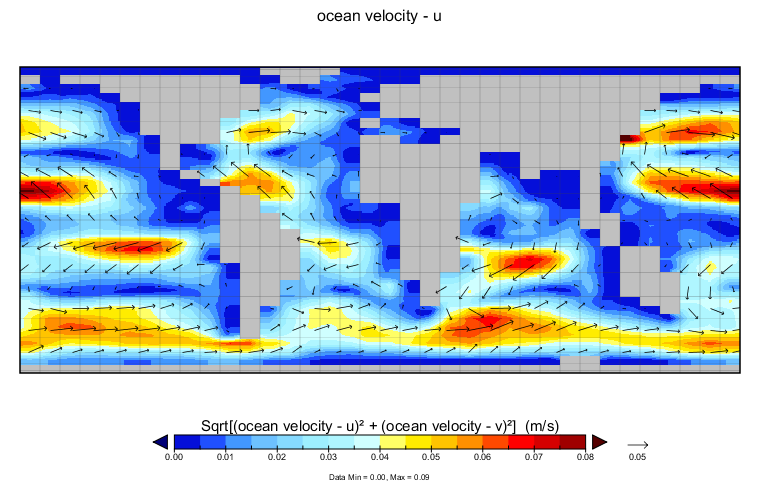
\includegraphics[width=0.6\textwidth]{ch3-currents1.png}\centering
\vspace{-0mm}
\caption{Example plot of (normal/default modern) ocean current fields (3D netCDF file). Again scaling has been set manually to create an easy-to-interpret axis scale. On the left is the surface field, and on the right an intermediate depth (illustrating what approximates the Deep Western Boundary current in the model in the Atlantic).}
\label{fig:ch3-currents1}
\end{figure}

%------------------------------------------------
\vspace{1mm}
\noindent\rule{4cm}{0.5pt}
\vspace{2mm}
%------------------------------------------------

\noindent The second approach is to visualize the large-scale ocean transport in terms of the meridional overturning circulation ('stream-function') (e.g. see background literature).

Two example plots (using \textbf{Panoply}) are shown in Figure \ref{fig:ch3-amoc1} for the Atlantic basin, and Figure \ref{fig:ch3-amoc2} for the Pacific. In the In the 2D \textbf{netCDF} file, relevant fields (netCDF variables)\footnote{Note that these fields are only meaningful for the modern arrangement of the continents and a continuous separation of the Atlantic from the Pacific from high northern latitudes down to the tip of South America. Different (e.g. paleo) arrangements of the continents may not have recognisable (or definable) Atlantic and/or Pacific basins and it may only be possible to define and visualize the global meridional overturning circulation -- variable: \textsf{\footnotesize phys\_opsi}.} are:
\begin{itemize}[noitemsep]
\setlength{\itemindent}{.0in}
\item [] \textsf{\footnotesize phys\_opsia} == global overturning stream-function
\item [] \textsf{\footnotesize phys\_opsip} == overturning in the Atlantic
\end{itemize}

\begin{figure}
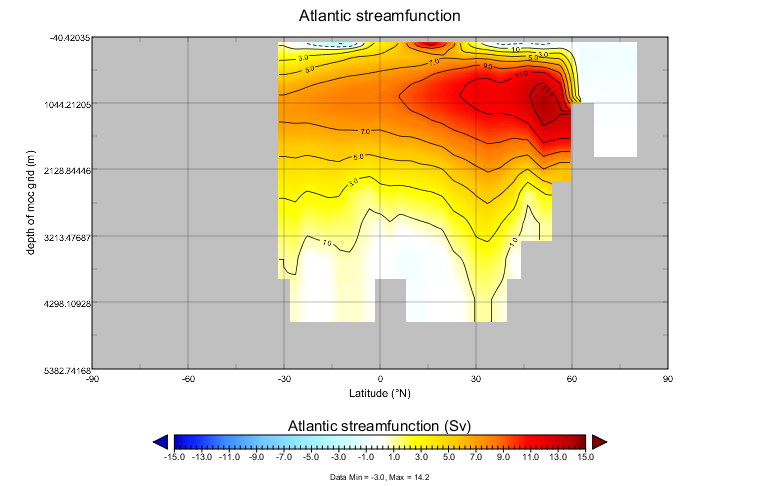
\includegraphics[width=0.6\textwidth]{ch3-amoc1.png}\centering
\vspace{-0mm}
\caption{Example plot of (normal/default modern) overturning stream-function (2D \textbf{netCDF} file). (e.g., for Atlantic: \textbf{netCDF} parameter name: \texttt{phys\_opsia}, long-name: Atlantic stream-function). Note that auto-scaling has been turned off and the min and max plotting limits set manually. By convention, stream-functions are plotted with their scale symmetrical around zero, giving red and ‘warm’ colors for positive value and clockwise overturning, and blues and ‘cold’ colors for negative values and anti-clockwise overturning. (The plot has been tart-ed up by overlaying solid contours plus contour labels.) It may be necessary in \textbf{Panoply} to re-orient (invert) the vertical grid.}
\label{fig:ch3-amoc1}
\end{figure}

\begin{figure}
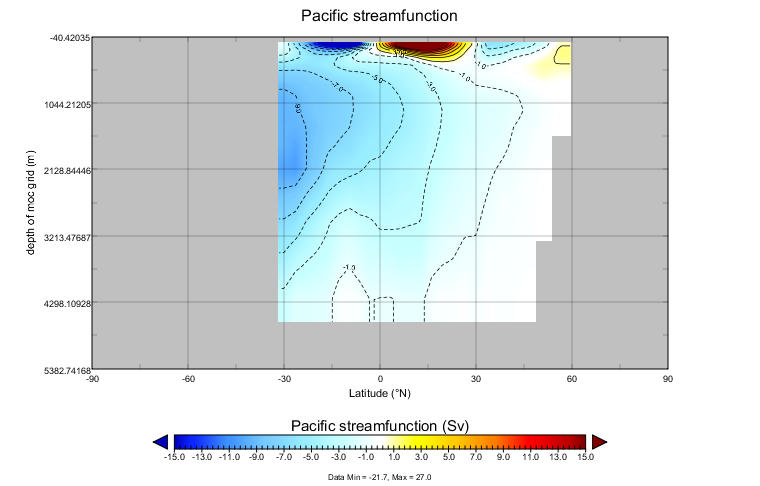
\includegraphics[width=0.6\textwidth]{ch3-amoc2.png}\centering
\vspace{-0mm}
\caption{Pacific meridional overturning circulation (PMOC).}
\label{fig:ch3-amoc2}
\end{figure}

%------------------------------------------------
\newpage
%------------------------------------------------

\section{Tracing ocean circulation}

The ocean biogeochemistry module (\textbf{BIOGEM}) in \textbf{cookie} provides a framework for applying time- and spatially-variable ‘forcings’ of the Earth system\footnote{Refer to the '\textit{force the system}' \textsf{HOW-TO} in the cookie manual for further details on \textit{forcings}.} – fluxes or 'restored-to' boundary conditions that can be prescribed for any gas, dissolved substance (including temperature and salinity), or particulate matter. Examples include freshwater input (== a negative salinity flux forcing) of the North Atlantic to alter ocean circulation, fossil fuel \(CO_{2}\) emissions to the atmosphere (== a \(CO_{2}\) gas flux forcing), or aeolian iron supply to the surface ocean (a 2-D dust flux forcing).

\vspace{1mm}
For example: view the \textit{user-config} file: \textsf{\footnotesize LAB.2.2.colortracer} – you will see the following lines (under the heading: ‘\texttt{\# --- FORCINGS ---}’)

\vspace{-2mm}\small
\begin{verbatim}
bg_par_forcing_name="pyyyyz_Fblue"
bg_par_force_point_i=22
bg_par_force_point_j=33
bg_par_force_point_k=8
bg_par_ocn_force_scale_val_49=1.0E12
\end{verbatim}
\normalsize\vspace{-2mm}

The first line points \textbf{cookie} to a directory located in \textsf{\footnotesize cgenie.cookie/genie-forcings} that contains a set of files that define what geochemical property is going to be altered plus information about how the magnitude of the forcing changes with time.

There are then three lines (\texttt{bg\_par\_force\_point\_i=20}, ...) that specify the location in the ocean of the geochemical forcing that is going to be applied. The point sources are specified in (i,j,k) coordinates, which in this case is (22,33,08). For the ocean model resolution we are using, the grid is 36x36x16, and in which: longitude (i) is counted from left-to-right (1 to 36); latitude (j) is counted from bottom-to-top (1 to 36); level depth (k) is counted from downwards top-to-bottom (16 down to 1). Thus, (22,33,08) is a release of tracer in the North Atlantic, a little south of Greenland, and intermediate depth (level = 8 out of 16). Refer to the Figures for how the horizontal (Figure \ref{fig:ch3-ijgrid}) and vertical (Figure \ref{fig:ch3-kgrid}) grid is specified.

Finally, there is a scaling parameter (\texttt{bg\_par\_ocn\_force\_scale\_val\_49}) which modifies the magnitude of the flux to be applied\footnote{Flux \textit{forcings} in \textbf{cookie} are in units of \(mol yr^{-1}\) per model grid point.} -- the default value in the forcing definition itself is just \(1.0 mol yr^{-1}\).

%------------------------------------------------
\newpage 
%------------------------------------------------

%
\begin{figure}
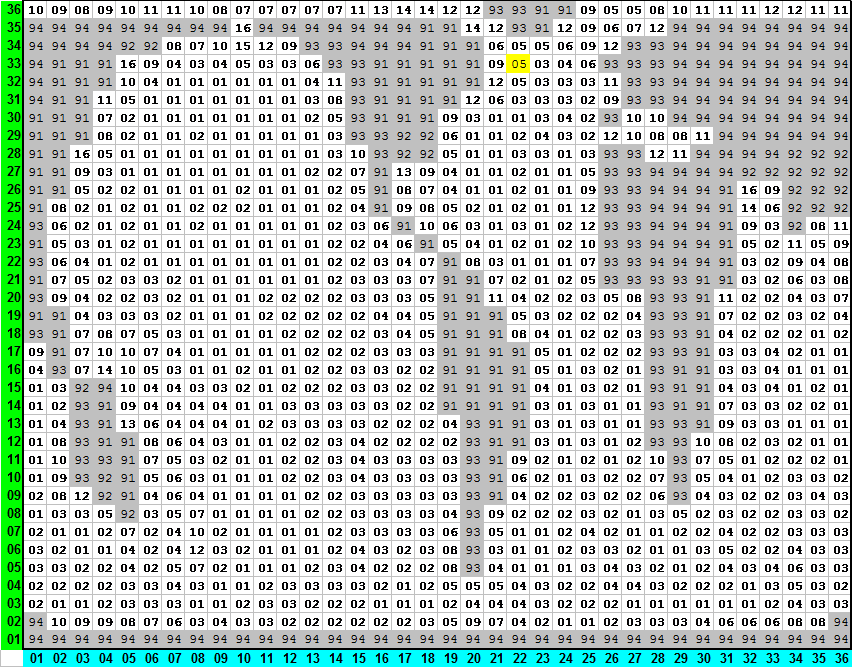
\includegraphics[width=0.8\textwidth]{ch3-ijgrid.png}\centering
\vspace{-0mm}
\caption{
\textbf{The  cookie grid for a modern \(36\times36\) ‘p\_worjh2’ configuration.} Light blue numbers are the ‘i’ co-ordinates. Green numbers are the ‘j’ co-ordinates.
The depth of the ocean at any location is indicated by its ‘k’ value – a number between 1 and 16, with 16 being the surface layer of the ocean, and 1 the maximum possible depth anywhere.
Numbers > 90 (91, 92, 93, 94) and shaded grey are land (and specify the direction of run-off).
Location (22,33,08) is highlighted in yellow.
The longitude of the western edge of this particular modern ocean grid is at 260$^{\circ}$W, and the increments are 10$^{\circ}$.
}
\label{fig:ch3-ijgrid}
\end{figure}

\begin{figure}
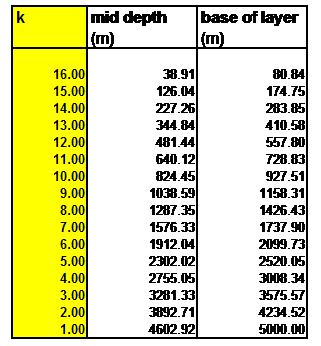
\includegraphics[width=0.4\textwidth]{ch3-kgrid.png}\centering
\vspace{-0mm}
\caption{\textbf{The cookie ocean vertical level definitions for a modern 16-level ocean grid.}}
\label{fig:ch3-kgrid}
\end{figure}

\noindent You are going to run a brief experiment in which you will be injecting a conservative ‘dye’ tracer into the ocean. The \textbf{BIOGEM} module has two tracers that can be defined for this purpose – ‘blue’ and ‘red’ -- you will be using the \uline{blue} one here. You can control the flux of blue dye by opening the \textit{user-config} file: \textsf{\footnotesize LAB.2.2.colortracer} and editing the flux scaling parameter:

\vspace{-2mm}\small\begin{verbatim}
bg_par_ocn_force_scale_val_49=1.0E12
\end{verbatim}\normalsize\vspace{-2mm}

\vspace{1mm}
The \textit{base-config} you will be using is different from previously: \textsf{\footnotesize cookie.C.p\_worjh2.rb} – this specifies a 16 vertical levels ocean and also includes seasonality of solar insolation.\footnote{Note that because the \textit{base-config} is different from that used in the previous chapter, you need to force a re-compile of the model code before any experiments can be submitted as cluster jobs. The easiest way to do this is to run an experiment interactively at the command line.}

%------------------------------------------------
\vspace{1mm}\noindent\rule{4cm}{0.5pt}\vspace{2mm}
%------------------------------------------------

%------------------------------------------------
\newpage 
%------------------------------------------------

\noindent Run the model for … whatever, 20 years will do. Use the \textit{re-start} experiment that you have just downloaded to start from:

\vspace{-2mm}\small\begin{verbatim}
$ ./runcookie.sh cookie.C.p_worjh2.rb LABS LAB.2.2.colortracer 20 
   cookie.C.p_worjh2.rb.SPIN
\end{verbatim}\normalsize\vspace{-2mm}

View the results – for instance how the blue tracer distribution evolves with time – in the \textit{time-slice} files (full ocean/atmosphere) properties saved in the \textbf{netCDF} format (\texttt{.nc}) files). You can follow the progress of the dye (and hence diagnose the properties of ocean circulation in the model) by plotting vertical and/or horizontal slices that go through (or near) the cell location in which you inject the dye tracer in the 3D \textbf{netCDF} file. Note that \textbf{Panoply} appears to ‘count’ the ocean layers in the opposite direction to the way in which the ocean model is actually counting them – the correct definition is with ‘1’ being very deepest level possible (and as displayed in the figure) and '16' is the surface.

You can also view the tracer distributions in terms of a water-column integrated tracer inventory (\textbf{netCDF} variable name: \textsf{\footnotesize ocn\_int\_colb}; long name: \textsf{\footnotesize colb water-column integrated tracer inventory}) in the 2D \textbf{netCDF} output. (See: \textit{Sabine et al.} [2004] for the use of water column integrals in the context of the distribution of anthropogenic \(CO_{2}\) uptake and storage.) Changes in tracer inventory with time can be tracked in the time-series file: \textsf{\footnotesize biogem\_series\_ocn\_colb.res}

Spend a little while altering the flux (\texttt{\small bg\_par\_ocn\_force\_scale\_val\_49}) and/or location
\\(\texttt{\small bg\_par\_force\_point\_i}, \texttt{\small bg\_par\_force\_point\_j, bg\_par\_force\_point\_k}) of tracer input. Overall -- note how you can use numerical ‘tracers’ to help diagnose (and better understand) the circulation of the ocean.

\large\uline{Ignore the 'red' tracer for now ... we'll look at that shortly.}\normalsize

%------------------------------------------------
\vspace{1mm}\noindent\rule{4cm}{0.5pt}\vspace{2mm}
%------------------------------------------------

%------------------------------------------------
\newpage 
%------------------------------------------------
%
\noindent When you add the numerical dye, particularly early on in the experiment, you may see a 'front' of \uline{negative} tracer concentrations leading the (positive) tracer as it spreads. DON'T PANIC!

The model is ... a model (of the numerical flavor) and not an exact analytical solution. So errors in how it solves ocean transport are to be expected.

Moreover, by default the ocean circulation model employs an isopycnal/diapycnal mixing scheme. This can lead to unwanted negative tracer values when sharp horizontal (or vertical) transitions in concentration occur. (In this example, e.g. by injection dye at a point location into a surrounding ocean of initially zero concentration.)

You can change to a simpler horizontal/vertical (.false.) mixing scheme by adding to the \textit{user-config} file:

\vspace{-2mm}\small\begin{verbatim}
# turn OFF (=.false.) isopycnal/diapycnal mixing
go_diso=.false.
\end{verbatim}\normalsize\vspace{-2mm}

If you try this, you should (hopefully) find much less (or no) negative tracer concentrations occur. However, also note that by changing the physics of ocean mixing, you also slightly alter the large-scale circulation of the ocean (and e.g. the AMOC might change slightly in strength).\footnote{You might contrast the overturning stream-functions for experiments run both with and without horizontal/vertical mixing.} 

%------------------------------------------------
\vspace{1mm}\noindent\rule{4cm}{0.5pt}\vspace{2mm}
%------------------------------------------------

\noindent Lastly, an interesting (honest!) and illustrative exercise is to use the dye tracer to pick out the path taken by Mediterranean Intermediate Water. Despite the low resolution of the \textbf{cookie} ocean circulation model component and the highly restricted representation of the Mediterranean, the model does project a salty Mediterranean as a consequence of  P-E across this basin (and its catchments) being negative and this higher density water makes its way out in the subsurface into the Atlantic.

To do this -- simply specify a dye injection somewhere in the Mediterranean (be careful with the restricted depth of the Mediterranean – if you inject too deeply (into the crust!) then you will not see anything (refer to the figure for the depth level (k) number of the maximum depth of the water column in each location), and it is better to inject it relatively close to the opening of the gateway (try some different locations and see which ones produce a reasonably instructive tracing of Mediterranean outflow). Run for e.g., 20 or 50 years (from the provided spin-up). Then:

\vspace{1mm}
\begin{enumerate}[noitemsep]
\vspace{1mm}
\item View the dye-tagged plume of Mediterranean Intermediate Water by plotting a lat-lon slice (from the 3D \textbf{netCDF} file). This will give you the depth of the plume. How does this compare with salinity observations (salinity observations and appropriate global data-sets can be found on the web with a little patience)? You can also view the water-column integrated distribution (2D \textbf{netCDF}).
\vspace{1mm}
\item Try viewing the plume via a lat-depth slice. Refer to the figure to determine the ‘i’ value up the Atlantic that will just graze the edge of what passes for Spain at this low model resolution. Which direction does it head after exiting the Mediterranean? Is this ‘realistic’?
\end{enumerate}
\vspace{1mm}

%------------------------------------------------
\newpage
%------------------------------------------------

\section{Tracing ocean ... ventilation}

Yet another way to think about global ocean circulation is through considering the connection (rate of mass exchange) between surface and deep ocean -- 'ventilation'.

\textbf{cookie} has the capability to employ/simulate a ventilation age tracer\footnote{Under the '\textit{screw with and/or diagnose the climate system}' HOW-DO -- see '\textit{Add a water mass age tracer}' (and the 'easy'/automatic method described towards the end of that section).} -- a numerical tracer carried in the ocean circulation model that tracks the time since a parcel of water last 'saw' the surface. The older the 'age' of the parcel of water, the longer the time since it last saw the surface.

We can use the second numerical tracer (red') to keep track of age, but rather than apply a flux forcing to the surface, we let the model automatically restore the tracer value at the surface to zero and everywhere else (in the ocean interior) increase the age each time-step (by the duration of the time-step) such that a parcel of water away from the surface ages by 1 year, each year.

The \textit{base-config}, and \textit{restart}, provided for the ('blue') circulation tracing, already has the ('red') age tracer included and activated. As a result, all of your experiments on ocean circulation which you have conducted so far already have simulated ocean ventilation age and you do not need to run a new experiment (unless you want to!).

%------------------------------------------------
\vspace{1mm}\noindent\rule{4cm}{0.5pt}\vspace{2mm}
%------------------------------------------------

\noindent In the 3D netCDF output file -- \textsf{\footnotesize misc\_col\_Dage} is the output variable that is the calculated ventilation age.

Explore the distribution of water mass age and think about the physical ocean circulations reasons for this. Are all the modelled distributions reasonable? Are there indicators of facets of the simulated circulation that are not particularly realistic? Try plotting both lon-lat and lat-depth slices through the ocean. How does the distribution of water mass age relate to the overturning stream-function for Atlantic or Pacific basins (more on this in the next Section)?

%------------------------------------------------
\newpage
%------------------------------------------------

\section{Poking the climate beast}

Instead of adding a dye tracer, you could add fresh water to the ocean surface to assess the sensitivity of the Atlantic Meridional Overturning Circulation (AMOC) to collapse, in a classic ‘hosing’ experiment.

The \textit{user-config} file for this is called: \textsf{\footnotesize LAB.2.4.hosing}. The default (i,j) location of the flux input is the same (as the dye tracer), but now the injection at the surface (level: k=16). Note that the forcing of the salinity tracer is negative (freshwater = negative salinity compared to sea-water)!

To orientate you in freshwater forcing space: \texttt{bg\_par\_ocn\_force\_scale\_val\_2=-2.0E17} should be sufficient to make ‘stuff happen’ and quickly. BUT, this is a pretty extreme flux (see overleaf for a rough conversion between salinity forcing units (mol yr$^{-1}$) and fresh water flux (in m$^{3}$ s$^{-1}$ or Sv). Much more than this and the model may crash or at the very least, you’ll be left with a large freshwater pond in the North Atlantic … (see later for some exciting discussion on units!)

\vspace{1mm}
To run the model for e.g., 20 years using the same restart:

\vspace{-2mm}\small\begin{verbatim}
$ ./runcookie.sh cookie.C.p_worjh2.rb LABS LAB.2.4.hosing 20 
   cookie.C.p_worjh2.rb.SPIN
\end{verbatim}\normalsize\vspace{-2mm}

\noindent 20 years should be long enough to see a collapse start to occur, but you might want to run the model for longer (and it can be submitted as a job, of course). Running for longer will also allow you to have a smaller, less extreme (and maybe more realistic) freshwater input flux.

Make sure that you run a \uline{control} experiment -- an experiment of the same duration of your hosing experiments, but with a zero freshwater flux. The impact of freshwater input, is the difference, at the same model year, between the perturbation experiment and the control. (You only ever need need to run one control, regardless of how many different freshwater flux perturbation experiments  you run.) 

Note that as the model is running rather s l o w e r than in the snowball configuration, you might want to think carefully of making use of cluster queuing possibilities (i.e., running multiple experiments at once in the background).

%------------------------------------------------
\vspace{1mm}\noindent\rule{4cm}{0.5pt}\vspace{2mm}
%------------------------------------------------

\noindent The most obvious property of the Earth system to follow is the Atlantic overturning strength (\textsf{\footnotesize biogem\_series\_misc\_opsi.res}). The AMOC stream-function (in \textsf{\footnotesize fields\_biogem\_2d.nc} 2-D time-slice \textbf{netCDF} results file, field: \textsf{\footnotesize phys\_opsia}) is also illustrative. You can also try and identify the salinity anomaly (see below) due to freshwater input in the 3D salinity tracer field.

There are also important (but not necessarily painfully exciting) impacts on surface air temperatures and maybe sea-ice extent (in \texttt{fields\_biogem\_2d.nc)} (but see below for a better way to visualize these changes). Note the importance (sort of) of the AMOC in transporting heat to the N Atlantic region (the film the Day After Tomorrow was not entirely inaccurate in this particular respect). Be aware of the possibility of climate impacts far from the location of fresh water forcing. Look out for any significant-looking impacts on sea-ice extent, etc.

You might also plot current velocity fields and visualize how these change in response to the fresh water forcing.

Lastly, if you ran much longer than 20 years, you might start to see impacts on the ocean ventilation age.

%------------------------------------------------
\vspace{1mm}\noindent\rule{4cm}{0.5pt}\vspace{2mm}
%------------------------------------------------

%------------------------------------------------
\newpage
%------------------------------------------------

\noindent To more easily assess some of these impacts (and for other sorts of analysis) it is possible to create an \uline{anomaly (difference) map} in \textbf{Panoply}:

\vspace{1mm}
\begin{enumerate}[noitemsep]
\vspace{1mm}
\item  First open a dataset, e.g., \textsf{\footnotesize atm\_temp} (surface air temperature) in the 2D \textbf{netCDF} file. You can either double-click the variable name, or, with the variable name highlighted, click the ‘Create Plot’ icon.
\vspace{1mm}
\item Now, with the \textsf{\footnotesize atm\_temp} still selected (and the first plot window still open), click on the ‘Combine Plot’ icon. A dialogue box will appear and ask you to select a plot to combine the new one with. Make sure the name of your first plot window is selected/highlighted. Click ‘Combine’. OR, simply drag a second dataset into the plot window of the first dataset.
\vspace{1mm}
\item You now have a plot window that by default it is showing you the difference between two identical (in time) slices. The two different slices are labeled Array 1 (LH side) and Array 2 (RH side).
\end{enumerate}
\vspace{1mm}

Keep one array (Array 1) fixed to the initial (year 1 (centered on 0.5)) and vary the year in the second array (Array 2). Note that you can select in Panoply whether Array 1 – Array 2 is plotted, or Array 2 – Array 1, or various proportional or relative differences.

Note that you can switch off the auto-scaling feature (Always fit to data) and center the scale so that no change is white, with positive deviations = red and negative = blue by clicking on Center on 0 (an often used convention in climate field plotting).

%------------------------------------------------
\vspace{1mm}\noindent\rule{4cm}{0.5pt}\vspace{2mm}
%------------------------------------------------

\noindent Finally, a brief note on units ... the freshwater forcing is implemented as negative salinity, just to really screw with your mind. The generic internal \textbf{cookie} model units for the forcing end up as \(PSU kg^{-1} yr^{-1}\). Which sort of does not make much sense ...

Start, by thinking of a value of \texttt{bg\_par\_ocn\_force\_scale\_val\_2} of \(-34.9\) as equivalent to taking all the salt out of \(1 kg\) of freshwater (since the mean global salinity is \(34.9 PSU\)). Or equivalently, since the ocean volume is fixed, an applied forcing value of \(-34.9\) is equivalent to adding \(1 kg\) of freshwater to a (surface) box. So, a value of \texttt{bg\_par\_ocn\_force\_scale\_val\_2} of \(-3.49\times10^{4}\) (\(-3.49E04)\) would be a flux of \(1 m^{3} yr^{-1}\) (\(1000 kg m^{-3}\)) of freshwater.

So, in the example earlier (\texttt{bg\_par\_ocn\_force\_scale\_val\_2=-1.0E18}), the freshwater flux is \(1.0\times10^{18}/3.49\times10^{4} = 2.8653\times10^{13} m^{3} yr^{-1}\).

The literature invariably gives freshwater fluxes in units of \(Sv\) (\(10^{6} m^{3} s^{-1}\)). So in the example, the freshwater flux is: \(9.0797\times10^{5} m^{3} s^{-1}\) (\(365.25\times24\times3600 = 31557600 s yr^{-1}\)). Or \(0.9 Sv\).

Or or ... \(1.0 Sv\) is equivalent to a model (\texttt{bg\_par\_ocn\_force\_scale\_val\_2}) total forcing flux of \(-1.0E18/0.90797 = -1.1E18\)

Read the literature … but generally, fluxes of ca. \(0.05 Sv\) and larger (and to quite specific places) are applied in models to induce an AMOC collapse.

%------------------------------------------------
\newpage
%------------------------------------------------

\section{Further ideas}

%------------------------------------------------

\subsection{Assessing the spatial sensitivity of deep-water formation to shutdown}

What is the largest freshwater flux that can be sustained without ‘collapsing’ the AMOC? Is there a ‘threshold’ (‘tipping point’) of freshwater input, beyond which the AMOC rapidly decreases in strength? For this -- you would run (submit to the cluster) a series of experiments, each with different (increasing) values for the fresh water flux. Remember to include an experiment with zero freshwater flux to act as a 'control'.

Is the precise location of the freshwater input important (i.e., try tipping it in somewhere else)? For this -- you could piece-meal run an experiment, analyse the results, then choose a new location to input the freshwater, or, come up with a systematic search pattern of freshwater input patterns.  

Outside of the North Atlantic, are any other  regions (of deep water formation) sensitive to freshwater perturbation and what are the consequences (could it happen in the future)?

%------------------------------------------------

\subsection{Forcing stronger deep-water formation (‘anti-hosing’ investigations)}

There are questions concerning past changes in the AMOC as to whether it is ‘pushed’ or ‘pulled’. i.e., if the AMOC shoals in depth and/or weakens, is it because its production has weakened, or as Antarctic Bottom water (AABW) strengthened and ‘pushed’ it out of the way (to shallower depths)?

What you might try then is to inject salt in the Southern Ocean as opposed to fresh water in the North Atlantic. All you need do is pick an appropriate grid point (this is worth thinking about carefully and maybe testing different locations) and rather than giving the parameter \texttt{bg\_par\_ocn\_force\_scale\_val\_2} a negative value, you give it a positive one. (Start by trying similar magnitudes of value as before and see what happens.)

\textbf{Is the AMOC (for the same magnitude of forcing) more sensitive to being ‘pushed’ or ‘pulled’?} (Obviously the answer will  depend on where the perturbations are being applied.)

%------------------------------------------------

\subsection{Response to transient warming}

A current concern regarding anthropogenic climate change is the ocean circulation (and marine ecological and biogeochemical) response to a strong warming of the surface, as rapid surface warming is assumed (and demonstrated in models) to result in surface stratification of the ocean, likely restricting the nutrient supply to phytoplankton and reducing ventilation of the ocean interior with dissolved oxygen.

You can explore the transient response of ocean circulation to warming by simply adjusting the radiative forcing parameter as per used in the snowball Earth experiments: \texttt{ea\_radfor\_scl\_co2}. By default in the modern continental configuration, this has a value of 1.0, corresponding to 278 ppm atmospheric \(CO_{2}\). A value of 2.0 would reflect warming equivalent to 556 ppm \(CO_{2}\). And 3.0 more like an end-of-the-century warming. Note that you are applying the warming instantaneously by manipulating the climate system in this way and hence the changes will be more extreme than those occurring over the time-scale of this century. Also note that a cooling (a radiative scaling small er than $1.0$) could be applied instead.

Potentially interesting properties of the Earth system to look at include sea-ice extent and AMOC strength (in the ASCII time-series files), and the overturning stream-function and sea-ice extent in the 2-D \textbf{netCDF} output. It is also possible to fresh water force the model with an age tracer and hence make projections of how patterns of ventilation age change with transient warming.

Overall, try and answer the question: \textbf{How much radiative forcing is required to collapse the AMOC? What atmospheric \(CO_{2}\) value does this approximately correspond to?}

%------------------------------------------------

\subsection{Regional hosing}

\noindent It is also possible to apply freshwater fluxes in a specific pattern/region, rather than just at a single location.

%----------------------------------------------------------------------------------------
%----------------------------------------------------------------------------------------
%----------------------------------------------------------------------------------------
%       CHAPTER 3
%----------------------------------------------------------------------------------------

\cleardoublepage

\chapterimage{middle_earth.png} % Chapter heading image

\chapter{Ocean circulation II (fake worlds)}\label{ch:ocean-circulation-II}

\hfill \break

%------------------------------------------------
\newpage
%------------------------------------------------

\section{(none)}

%----------------------------------------------------------------------------------------
%----------------------------------------------------------------------------------------
%%----------------------------------------------------------------------------------------
%       CHAPTER 3
%----------------------------------------------------------------------------------------

\cleardoublepage

\chapterimage{amoc.png} % Chapter heading image

\chapter{Ocean circulation}\label{ch:ocean-circulation}

\hfill \break

\noindent Stuff to keep in mind:

\begin{itemize}
\item Nothing at all – keep your mind completely empty and let the wonderful truths of \textbf{muffin} permeate your entire being.
\end{itemize}

\vspace{2mm}
\noindent Background reading (Atlantic circulation and stability in \textbf{muffin}):

\vspace{2mm}
\begin{itemize}
\item Hargreaves et al. [2004] (Climate Dynamics 23, 2004, Pages 745 – 760)
\\\(\rightarrow\)Simple assessment of the likelihood of AMOC collapse.
\item Marsh et al. [2004] (Climate Dynamics, 23 2004, Pages 761 – 777)
\\\(\rightarrow\)Characterization of thresholds of AMOC collapse.
\item Singaraye et al. [2008] (GRL 35, doi:10.1029/2008GL034074)
\\\(\rightarrow\)Role of changing ocean circulation in atmospheric radiocarbon variability during the Younger Dryas.
\end{itemize}

\vspace{2mm}
\noindent Background reading (Miscellaneous (model) Atlantic circulation and stability):

\vspace{2mm}
\begin{itemize}
\item IPCC [2007] (e.g., Section 10.3.4)
\\\(\rightarrow\)Future predictions of AMOC strength.
\item Schmittner [2005] (Nature 434, 628– 633)
\\\(\rightarrow\)Impacts on marine ecosystems and carbon cycling.
\item Obata [2007] (J. Clim. 20, 5962–5976)
\\\(\rightarrow\)Climate-carbon cycle model response to freshwater discharge.
\end{itemize}

%------------------------------------------------
\newpage
%------------------------------------------------

\section*{READ.ME}

You will need to download a new \textit{re-start} file prior to embarking on the experiments with modern ocean circulation.
To fetch this: change to the \texttt{cgenie\_output} directory, and type (or copy and paste carefully from the PDF ...):

\vspace{-2mm}
\small\begin{verbatim}
$ wget --no-check-certificate http://www.seao2.info/cgenie_output/LAB_2.SPIN.tar.gz
\end{verbatim}\normalsize
\vspace{-2mm}

This downloads an archived/compressed copy of the 10,000 year \textit{spin-up} experiment \texttt{LAB\_2.SPIN}. Extract the contents of this archive by typing:

\vspace{-2mm}
\begin{verbatim}
$ tar xfzv LAB_2.SPIN.tar.gz
\end{verbatim}
\vspace{-2mm}

You’ll then need to change directory back to \texttt{genie-main} to run the model.

%------------------------------------------------
\newpage
%------------------------------------------------

\section{Visualizing ocean circulation}

Visualizing the 3D flow (/transport) of the ocean, much less the rate at which this occurs, is no trivial matter. Even with the aid of a model. (Or rather, the problem then becomes: how to visualize ocean circulation in a model.) We'll consider two different ways of analysing model velocity fields first -- simply utilizing the \textit{restart} that you have downloaded and unpacked, and then later take a more pro-active approach in subsequent Sections with some new experiments.

\vspace{1mm}
\noindent\rule{4cm}{0.5pt}
\vspace{2mm}

\noindent The first approach we can take is to simply visualize the raw velocity fields, but plotted as ocean currents.\vspace{1mm}
\begin{enumerate}[noitemsep]
\vspace{1mm}
\item  In the 3D \textbf{netCDF} file, the three components of ocean velocity are represented by the variables: ocean velocity – u (Eastwards), ocean velocity – v (Northwards), and ocean velocity – w (upwards). 2. Open up velocity – u. Chose ‘lon-lat’.
\vspace{1mm}
\item Select/highlight velocity – v. and click on the ‘Combine Plot’ icon (as per before).
\vspace{1mm}
\item Rather than a difference map, which is what you get by default, i.e., ‘Array 1 – Array 2’ – from the drop-down menu (next to the ‘Interpolate’ button) select ‘Vector Magnitude’.
\vspace{1mm}
\item You should have a color contoured (or not if you prefer plotting without contouring on) map of ocean current speed, with velocity vectors (direction and magnitude) overlain. You’ll need to re-scale the velocity vectors to properly see them – from the ‘Contours and Vectors’ tab – change the ‘Scale Length’ to e.g., 0.1. (On a \textbf{Mac}, look under the ‘Vectors’ tab for a ‘Reference Value’ to something like 0.1.)  When fresh-water hosing – look out for impacts on the N. Atlantic current system associated with the AMOC.
\vspace{1mm}
\item You can repeat this for deeper depth levels in the ocean – e.g., between about 1500 and 2000 m is a good place to go looking for the Western boundary current (and AMOC return) in the model (such as it exists at this low resolution) but you’ll need to re-scale the velocity vectors again (e.g., to 0.01 to less).
\end{enumerate}
\vspace{1mm}

\noindent An example plot (using \textbf{Panoply} for visualizing surface ocean current fields) is given in Figure \ref{fig:ch3-currents1}.

\begin{figure}
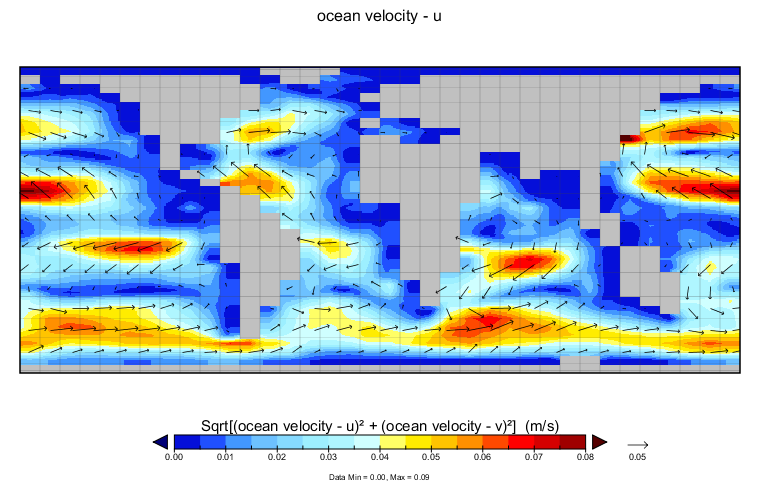
\includegraphics[width=0.6\textwidth]{ch3-currents1.png}\centering
\vspace{-0mm}
\caption{Example plot of (normal/default modern) ocean current fields (3D netCDF file). Again scaling has been set manually to create an easy-to-interpret axis scale. On the left is the surface field, and on the right an intermediate depth (illustrating what approximates the Deep Western Boundary current in the model in the Atlantic).}
\label{fig:ch3-currents1}
\end{figure}

%------------------------------------------------
\vspace{1mm}
\noindent\rule{4cm}{0.5pt}
\vspace{2mm}
%------------------------------------------------

\noindent The second approach is to visualize the large-scale ocean transport in terms of the meridional overturning circulation ('stream-function') (e.g. see background literature).

Two example plots (using \textbf{Panoply}) are shown in Figure \ref{fig:ch3-amoc1} for the Atlantic basin, and Figure \ref{fig:ch3-amoc2} for the Pacific. In the In the 2D \textbf{netCDF} file, relevant fields (netCDF variables)\footnote{Note that these fields are only meaningful for the modern arrangement of the continents and a continuous separation of the Atlantic from the Pacific from high northern latitudes down to the tip of South America. Different (e.g. paleo) arrangements of the continents may not have recognisable (or definable) Atlantic and/or Pacific basins and it may only be possible to define and visualize the global meridional overturning circulation -- variable: \textsf{\footnotesize phys\_opsi}.} are:
\begin{itemize}[noitemsep]
\setlength{\itemindent}{.0in}
\item [] \textsf{\footnotesize phys\_opsia} == global overturning stream-function
\item [] \textsf{\footnotesize phys\_opsip} == overturning in the Atlantic
\end{itemize}

\begin{figure}
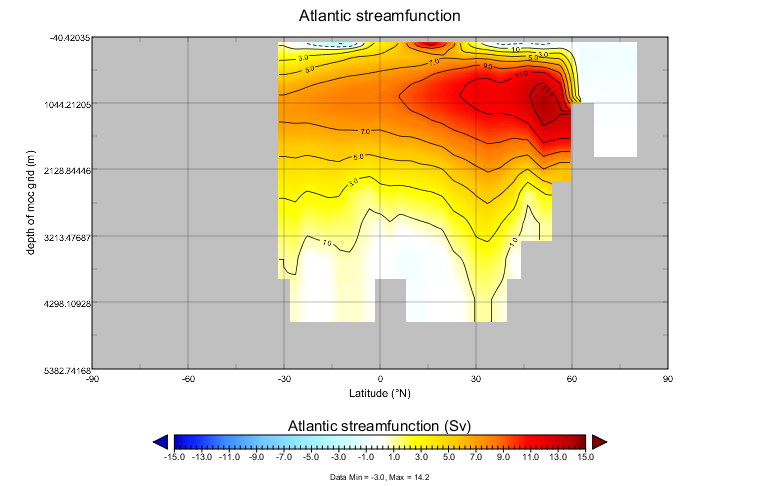
\includegraphics[width=0.6\textwidth]{ch3-amoc1.png}\centering
\vspace{-0mm}
\caption{Example plot of (normal/default modern) overturning stream-function (2D \textbf{netCDF} file). (e.g., for Atlantic: \textbf{netCDF} parameter name: \texttt{phys\_opsia}, long-name: Atlantic stream-function). Note that auto-scaling has been turned off and the min and max plotting limits set manually. By convention, stream-functions are plotted with their scale symmetrical around zero, giving red and ‘warm’ colors for positive value and clockwise overturning, and blues and ‘cold’ colors for negative values and anti-clockwise overturning. (The plot has been tart-ed up by overlaying solid contours plus contour labels.) It may be necessary in \textbf{Panoply} to re-orient (invert) the vertical grid.}
\label{fig:ch3-amoc1}
\end{figure}

\begin{figure}
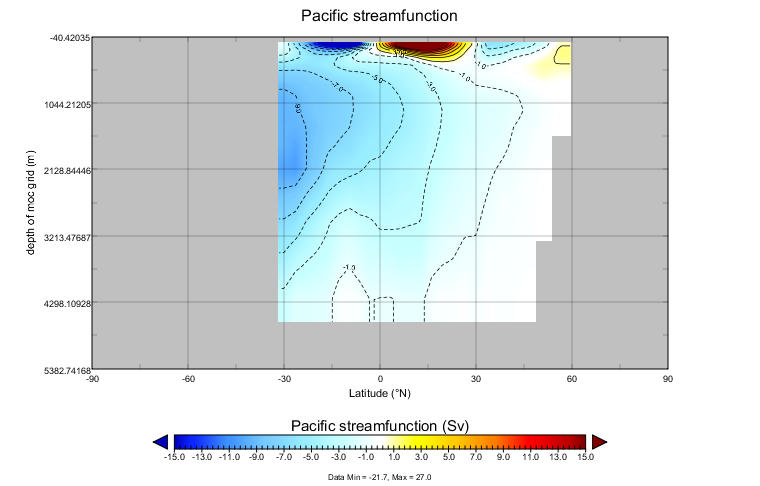
\includegraphics[width=0.6\textwidth]{ch3-amoc2.png}\centering
\vspace{-0mm}
\caption{Pacific meridional overturning circulation (PMOC).}
\label{fig:ch3-amoc2}
\end{figure}

%------------------------------------------------
\newpage
%------------------------------------------------

\section{Tracing ocean circulation}

The ocean biogeochemistry module (\textbf{BIOGEM}) in \textbf{muffin} provides a framework for applying time- and spatially-variable ‘forcings’ of the Earth system\footnote{Refer to the '\textit{force the system}' \textsf{HOW-TO} in the muffin manual for further details on \textit{forcings}.} – fluxes or 'restored-to' boundary conditions that can be prescribed for any gas, dissolved substance (including temperature and salinity), or particulate matter. Examples include freshwater input (== a negative salinity flux forcing) of the North Atlantic to alter ocean circulation, fossil fuel \(CO_{2}\) emissions to the atmosphere (== a \(CO_{2}\) gas flux forcing), or aeolian iron supply to the surface ocean (a 2-D dust flux forcing).

\vspace{1mm}
For example: view the \textit{user-config} file: \textsf{\footnotesize LAB\_2.colorinjection} – you will see the following lines (under the heading: ‘\texttt{\# --- FORCINGS ---}’)

\vspace{-2mm}\small
\begin{verbatim}
bg_par_forcing_name="pyyyyz_Fred"
bg_par_force_point_i=22
bg_par_force_point_j=33
bg_par_force_point_k=8
bg_par_ocn_force_scale_val_48=0.0
\end{verbatim}
\normalsize\vspace{-2mm}

The first line points \textbf{muffin} to a directory located in \textsf{\footnotesize cgenie.muffin/genie-forcings} that contains a set of files that define what geochemical property is going to be altered plus information about how the magnitude of the forcing changes with time.

There are then three lines (\texttt{bg\_par\_force\_point\_i=20}, ...) that specify the location in the ocean of the geochemical forcing that is going to be applied. The point sources are specified in (i,j,k) coordinates, which in this case is (22,33,08). For the ocean model resolution we are using, the grid is 36x36x16, and in which: longitude (i) is counted from left-to-right (1 to 36); latitude (j) is counted from bottom-to-top (1 to 36); level depth (k) is counted from downwards top-to-bottom (16 down to 1). Thus, (22,33,08) is a release of tracer in the North Atlantic, a little south of Greenland, and intermediate depth (level = 8 out of 16). Refer to the Figures for how the horizontal (Figure \ref{fig:ch3-ijgrid}) and vertical (Figure \ref{fig:ch3-kgrid}) grid is specified.

Finally, there is a scaling parameter (\texttt{bg\_par\_ocn\_force\_scale\_val\_48}) which modifies the magnitude of the flux to be applied (in units of \(mol yr^{-1}\) per model grid point).

%------------------------------------------------
\newpage 
%------------------------------------------------

%
\begin{figure}
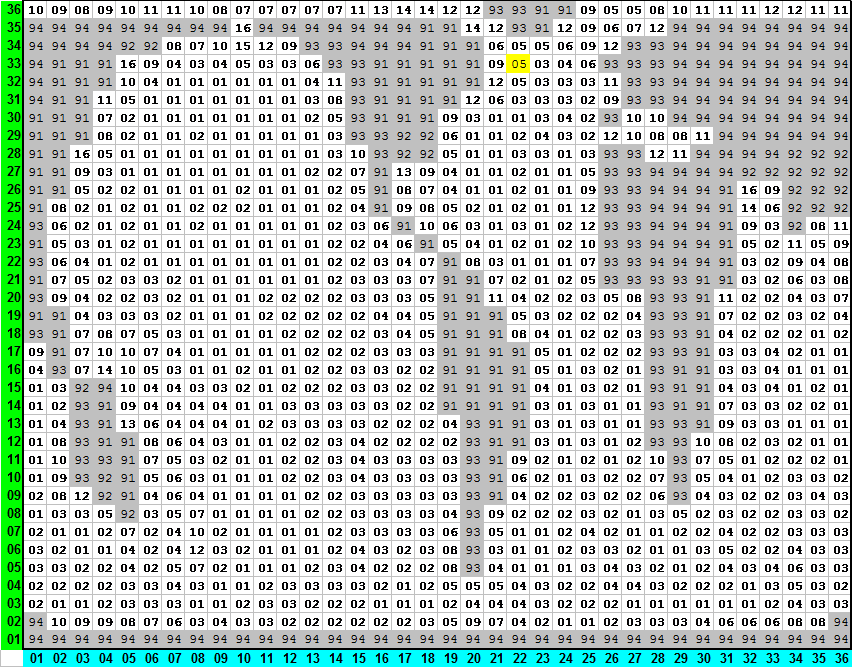
\includegraphics[width=0.8\textwidth]{ch3-ijgrid.png}\centering
\vspace{-0mm}
\caption{
\textbf{The  muffin grid for a modern \(36\times36\) ‘worjh2’ configuration.} Light blue numbers are the ‘i’ co-ordinates. Green numbers are the ‘j’ co-ordinates.
The depth of the ocean at any location is indicated by its ‘k’ value – a number between 1 and 16, with 16 being the surface layer of the ocean, and 1 the maximum possible depth anywhere.
Numbers > 90 (91, 92, 93, 94) and shaded grey are land (and specify the direction of run-off).
Location (22,33,08) is highlighted in yellow.
The longitude of the western edge of this particular modern ocean grid is at 260W, and the increments are 10 degrees.
}
\label{fig:ch3-ijgrid}
\end{figure}

\begin{figure}
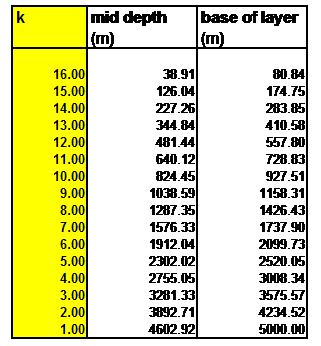
\includegraphics[width=0.4\textwidth]{ch3-kgrid.png}\centering
\vspace{-0mm}
\caption{\textbf{The muffin ocean vertical level definitions for a modern 16-level ocean grid.}}
\label{fig:ch3-kgrid}
\end{figure}

\noindent You are going to run a brief experiment in which you will be injecting a conservative ‘dye’ tracer into the ocean. The \textbf{BIOGEM} module has two tracers defined for this purpose – ‘blue’ and ‘red’. Open the \textit{user-config} file: \textsf{\footnotesize LAB\_2.colorinjection} and edit the parameter controlling the flux of red dye to read:

\vspace{-2mm}\small
\begin{verbatim}
bg_par_ocn_force_scale_val_48=1.0E12
\end{verbatim}
\normalsize\vspace{-2mm}

\noindent which specifies a flux of \(1.0\times10^{12}\) ( \(mol yr^{-1}\)) rather than zero as given as the default in the example \textit{user-config} file\footnote{i.e. don't leave the value as zero ... otherwise you'll have no flux forcing applied and will not see anything happen ...}.

\vspace{1mm}
The \textit{base-config} you will be using is different from previously: \textsf{\footnotesize cgenie.eb\_go\_gs\_ac\_bg.worjh2.rb} – this specifies a 16 vertical levels ocean and also includes seasonality of solar insolation.\footnote{Note that because the \textit{base-config} is different from that used in the previous chapter, you need to force a re-compile of the model code before any experiments can be submitted as cluster jobs. The easiest way to do this is to run an experiment interactively at the command line.}

%------------------------------------------------
\vspace{1mm}
\noindent\rule{4cm}{0.5pt}
\vspace{2mm}
%------------------------------------------------

%------------------------------------------------
\newpage 
%------------------------------------------------

\noindent Run the model for … whatever, 20 years will do. Use the \textit{re-start} experiment that you have just downloaded to start from:

\vspace{-2mm}\small
\begin{verbatim}
$ ./runmuffin.sh cgenie.eb_go_gs_ac_bg.worjh2.rb LABS LAB_2.colorinjection 20 LAB_2.SPIN
\end{verbatim}
\normalsize\vspace{-2mm}

View the results – for instance how the red tracer distribution evolves with time – in the \textit{time-slice} files (full ocean/atmosphere) properties saved in the \textbf{netCDF} format (\texttt{.nc}) files). You can follow the progress of the dye (and hence diagnose the properties of ocean circulation in the model) by plotting vertical and/or horizontal slices that go through (or near) the cell location in which you inject the dye tracer in the 3D \textbf{netCDF} file. Note that \textbf{Panoply} appears to ‘count’ the ocean layers in the opposite direction to the way in which the ocean model is actually counting them – the correct definition is with ‘1’ being very deepest level possible (and as displayed in the figure) and '16' is the surface.

You can also view the tracer distributions in terms of a water-column integrated tracer inventory (\textbf{netCDF} variable name: \textsf{\footnotesize ocn\_int\_colr}; long name: \textsf{\footnotesize colr water-column integrated tracer inventory}) in the 2D \textbf{netCDF} output. (See: \textit{Sabine et al.} [2004] for the use of water column integrals in the context of the distribution of anthropogenic \(CO_{2}\) uptake and storage.) Changes in tracer inventory with time can be tracked in the time-series file:

\vspace{-2mm}\small
\begin{verbatim}
biogem_series_ocn_colr.res.
\end{verbatim}
\normalsize\vspace{-2mm}

Spend a little while altering the flux (\texttt{\small bg\_par\_ocn\_force\_scale\_val\_48}) and/or location
\\(\texttt{\small bg\_par\_force\_point\_i}, \texttt{\small bg\_par\_force\_point\_j, bg\_par\_force\_point\_k}) of tracer input. Overall -- note how you can use numerical ‘tracers’ to help diagnose (and better understand) the circulation of the ocean.

%------------------------------------------------
\vspace{1mm}
\noindent\rule{4cm}{0.5pt}
\vspace{2mm}
%------------------------------------------------

%------------------------------------------------
\newpage 
%------------------------------------------------
%
\noindent When you add the numerical dye, particularly early on in the experiment, you may see a 'front' of \uline{negative} tracer concentrations leading the (positive) tracer as it spreads. DON'T PANIC!

The model is ... a model (of the numerical flavor) and not an exact analytical solution. So errors in how it solves ocean transport are to be expected.

Moreover, by default the ocean circulation model employs an isopycnal/diapycnal mixing scheme. This can lead to unwanted negative tracer values when sharp horizontal (or vertical) transitions in concentration occur. (In this example, e.g. by injection dye at a point location into a surrounding ocean of initially zero concentration.)

You can change to a simpler horizontal/vertical (.false.) mixing scheme by adding to the \textit{user-config} file:

\vspace{-2mm}\small
\begin{verbatim}
# turn OFF (=.false.) isopycnal/diapycnal mixing
go_diso=.false.
\end{verbatim}
\normalsize\vspace{-2mm}

If you try this, you should (hopefully) find much less (or no) negative tracer concentrations occur. However, also note that by changing the physics of ocean mixing, you also slightly alter the large-scale circulation of the ocean (and e.g. the AMOC might change slightly in strength).\footnote{You might contrast the overturning stream-functions for experiments run both with and without horizontal/vertical mixing.} 

%------------------------------------------------
\vspace{1mm}
\noindent\rule{4cm}{0.5pt}
\vspace{2mm}
%------------------------------------------------

\noindent Lastly, an interesting (honest!) and illustrative exercise is to use the dye tracer to pick out the path taken by Mediterranean Intermediate Water. Despite the low resolution of the \textbf{muffin} ocean circulation model component and the highly restricted representation of the Mediterranean, the model does project a salty Mediterranean as a consequence of  P-E across this basin (and its catchments) being negative and this higher density water makes its way out in the subsurface into the Atlantic.

To do this -- simply specify a dye injection somewhere in the Mediterranean (be careful with the restricted depth of the Mediterranean – if you inject too deeply (into the crust!) then you will not see anything (refer to the figure for the depth level (k) number of the maximum depth of the water column in each location), and it is better to inject it relatively close to the opening of the gateway (try some different locations and see which ones produce a reasonably instructive tracing of Mediterranean outflow). Run for e.g., 20 or 50 years (from the provided spin-up). Then:

\vspace{1mm}
\begin{enumerate}[noitemsep]
\vspace{1mm}
\item View the dye-tagged plume of Mediterranean Intermediate Water by plotting a lat-lon slice (from the 3D \textbf{netCDF} file). This will give you the depth of the plume. How does this compare with salinity observations (salinity observations and appropriate global data-sets can be found on the web with a little patience)? You can also view the water-column integrated distribution (2D \textbf{netCDF}).
\vspace{1mm}
\item Try viewing the plume via a lat-depth slice. Refer to the figure to determine the ‘i’ value up the Atlantic that will just graze the edge of what passes for Spain at this low model resolution. Which direction does it head after exiting the Mediterranean? Is this ‘realistic’?
\end{enumerate}
\vspace{1mm}

%------------------------------------------------
\newpage
%------------------------------------------------

\section{Tracing ocean ... ventilation}

Yet another way to think about global ocean circulation is through considering the connection (rate of mass exchange) between surface and deep ocean -- 'ventilation'.

\textbf{muffin} has the capability to employ/simulate a ventilation age tracer\footnote{Under the '\textit{screw with and/or diagnose the climate system}' HOW-DO -- see '\textit{Add a water mass age tracer}' (and the 'easy'/automatic method described towards the end of that section).} -- a numerical tracer carried in the ocean circulation model that tracks the time since a parcel of water last 'saw' the surface. The older the 'age' of the parcel of water, the longer the time since it last saw the surface.

We can use the same 'red' numerical tracer to keep track of age, but rather than apply a flux forcing to the surface, we let the model automatically restore the tracer value at the surface to zero and everywhere else (in the ocean interior) increase the age each time-step (by the duration of the time-step) such that a parcel of water away from the surface ages by 1 year, each year.

%------------------------------------------------
\vspace{1mm}
\noindent\rule{4cm}{0.5pt}
\vspace{2mm}
%------------------------------------------------

\noindent Provided is a  \textit{user-config} file for including an age tracer in the model: \textsf{\footnotesize LAB\_2.age}. You will also need a new \textit{re-start} experiment, called: \texttt{muffin.C.p\_worjh2.r.SPIN} and which can be downloaded and unpacked as per before (both from \textsf{\footnotesize cgenie\_output)}:

\vspace{-1mm}\small
\begin{verbatim}
$ wget --no-check-certificate 
     http://www.seao2.info/cgenie_output/muffin.C.p_worjh2.r.SPIN.tar.gz
\end{verbatim}
\normalsize\vspace{-1mm}
(all one line) and then:
\vspace{-1mm}\small
\begin{verbatim}
$ tar xfzv muffin.C.p_worjh2.r.SPIN.tar.gz
\end{verbatim}
\normalsize\vspace{-1mm}

To run (e.g. for 10 years), following on from its \textit{re-start} experiment, would be:

\vspace{-1mm}\small
\begin{verbatim}
$ ./runmuffin.sh cgenie.eb_go_gs_ac_bg.worjh2.rb LABS LAB_2.age 10
     muffin.C.p_worjh2.r.SPIN
\end{verbatim}
\normalsize\vspace{-1mm}

In the 3D netCDF output file -- \textsf{\footnotesize misc\_col\_Dage} is the output variable that is the calculated ventilation age.

Explore the distribution of water mass age and think about the physical ocean circulations reasons for this. Are all the modelled distributions reasonable? Are there indicators of facets of the simulated circulation that are not particularly realistic? Try plotting both lon-lat and lat-depth slices through the ocean. How does the distribution of water mass age relate to the overturning stream-function for Atlantic or Pacific basins (more on this in the next Section)?

%------------------------------------------------
\newpage
%------------------------------------------------

\section{Poking the climate beast}

Instead of adding a dye tracer, you could add fresh water to the ocean surface to assess the sensitivity of the Atlantic Meridional Overturning Circulation (AMOC) to collapse, in a classic ‘hosing’ experiment.

The \textit{user-config} file for this is called: \texttt{LAB\_2.hosing}. The default (i,j) location of the flux input is the same (as the dye tracer), but now the injection at the surface (level: k=16). Note that the forcing of the salinity tracer is negative (freshwater = negative salinity compared to sea-water)!

To orientate you in freshwater forcing space: \texttt{bg\_par\_ocn\_force\_scale\_val\_2=-2.0E17} should be sufficient to make ‘stuff happen’ and quickly. BUT, this is a pretty extreme flux (see overleaf for a rough conversion between salinity forcing units (mol yr$^{-1}$) and fresh water flux (in m$^{3}$ s$^{-1}$ or Sv). Much more than this and the model may crash or at the very least, you’ll be left with a large freshwater pond in the North Atlantic … (see later for some exciting discussion on units!)

\vspace{1mm}
To run the model for e.g., 20 years using the same restart:

\vspace{-2mm}\small
\begin{verbatim}
$ ./runmuffin.sh cgenie.eb_go_gs_ac_bg.worjh2.rb LABS LAB_2.hosing 20 LAB_2.SPIN
\end{verbatim}
\normalsize\vspace{-2mm}

\noindent 20 years should be long enough to see a collapse start to occur, but you might want to run the model for longer (and it can be submitted as a job, of course). Running for longer will also allow you to have a smaller, less extreme (and maybe more realistic) freshwater input flux.

Make sure that you run a \uline{control} experiment -- an experiment of the same duration of your hosing experiments, but with a zero freshwater flux. The impact of freshwater input, is the difference, at the same model year, between the perturbation experiment and the control. (You only ever need need to run one control, regardless of how many different freshwater flux perturbation experiments  you run.) 

Note that as the model is running rather s l o w e r than in the snowball configuration, you might want to think carefully of making use of cluster queuing possibilities (i.e., running multiple experiments at once in the background).

%------------------------------------------------
\vspace{1mm}
\noindent\rule{4cm}{0.5pt}
\vspace{2mm}
%------------------------------------------------

\noindent The most obvious property of the Earth system to follow is the Atlantic overturning strength (\textsf{\footnotesize biogem\_series\_misc\_opsi.res}). The AMOC stream-function (in \textsf{\footnotesize fields\_biogem\_2d.nc} 2-D time-slice \textbf{netCDF} results file, field: \textsf{\footnotesize phys\_opsia}) is also illustrative. You can also try and identify the salinity anomaly (see below) due to freshwater input in the 3D salinity tracer field.

There are also important (but not necessarily painfully exciting) impacts on surface air temperatures and maybe sea-ice extent (in \texttt{fields\_biogem\_2d.nc)} (but see below for a better way to visualize these changes). Note the importance (sort of) of the AMOC in transporting heat to the N Atlantic region (the film the Day After Tomorrow was not entirely inaccurate in this particular respect). Be aware of the possibility of climate impacts far from the location of fresh water forcing. Look out for any significant-looking impacts on sea-ice extent, etc.

You might also plot current velocity fields and visualize how these change in response to the fresh water forcing. 

%------------------------------------------------
\vspace{1mm}
\noindent\rule{4cm}{0.5pt}
\vspace{2mm}
%------------------------------------------------

%------------------------------------------------
\newpage
%------------------------------------------------

\noindent To more easily assess some of these impacts (and for other sorts of analysis) it is possible to create an \uline{anomaly (difference) map} in \textbf{Panoply}:

\vspace{1mm}
\begin{enumerate}[noitemsep]
\vspace{1mm}
\item  First open a dataset, e.g., \textsf{\footnotesize atm\_temp} (surface air temperature) in the 2D \textbf{netCDF} file. You can either double-click the variable name, or, with the variable name highlighted, click the ‘Create Plot’ icon.
\vspace{1mm}
\item Now, with the \textsf{\footnotesize atm\_temp} still selected (and the first plot window still open), click on the ‘Combine Plot’ icon. A dialogue box will appear and ask you to select a plot to combine the new one with. Make sure the name of your first plot window is selected/highlighted. Click ‘Combine’. OR, simply drag a second dataset into the plot window of the first dataset.
\vspace{1mm}
\item You now have a plot window that by default it is showing you the difference between two identical (in time) slices. The two different slices are labeled Array 1 (LH side) and Array 2 (RH side).
\end{enumerate}
\vspace{1mm}

Keep one array (Array 1) fixed to the initial (year 1 (centered on 0.5)) and vary the year in the second array (Array 2). Note that you can select in Panoply whether Array 1 – Array 2 is plotted, or Array 2 – Array 1, or various proportional or relative differences.

Note that you can switch off the auto-scaling feature (Always fit to data) and center the scale so that no change is white, with positive deviations = red and negative = blue by clicking on Center on 0 (an often used convention in climate field plotting).

%------------------------------------------------
\vspace{1mm}
\noindent\rule{4cm}{0.5pt}
\vspace{2mm}
%------------------------------------------------

\noindent Finally, a brief note on units ... the freshwater forcing is implemented as negative salinity, just to really screw with your mind. The generic internal \textbf{muffin} model units for the forcing end up as \(PSU kg^{-1} yr^{-1}\). Which sort of does not make much sense ...

Start, by thinking of a value of \texttt{bg\_par\_ocn\_force\_scale\_val\_2} of \(-34.9\) as equivalent to taking all the salt out of \(1 kg\) of freshwater (since the mean global salinity is \(34.9 PSU\)). Or equivalently, since the ocean volume is fixed, an applied forcing value of \(-34.9\) is equivalent to adding \(1 kg\) of freshwater to a (surface) box. So, a value of \texttt{bg\_par\_ocn\_force\_scale\_val\_2} of \(-3.49\times10^{4}\) (\(-3.49E04)\) would be a flux of \(1 m^{3} yr^{-1}\) (\(1000 kg m^{-3}\)) of freshwater.

So, in the example earlier (\texttt{bg\_par\_ocn\_force\_scale\_val\_2=-1.0E18}), the freshwater flux is \(1.0\times10^{18}/3.49\times10^{4} = 2.8653\times10^{13} m^{3} yr^{-1}\).

The literature invariably gives freshwater fluxes in units of \(Sv\) (\(10^{6} m^{3} s^{-1}\)). So in the example, the freshwater flux is: \(9.0797\times10^{5} m^{3} s^{-1}\) (\(365.25\times24\times3600 = 31557600 s yr^{-1}\)). Or \(0.9 Sv\).

Or or ... \(1.0 Sv\) is equivalent to a model (\texttt{bg\_par\_ocn\_force\_scale\_val\_2}) total forcing flux of \(-1.0E18/0.90797 = -1.1E18\)

Read the literature … but generally, fluxes of ca. \(0.05 Sv\) and larger (and to quite specific places) are applied in models to induce an AMOC collapse.

%------------------------------------------------
\newpage
%------------------------------------------------

\section{Further ideas}

%------------------------------------------------

\subsection{Hosing investigations}

What is the largest freshwater flux that can be sustained without ‘collapsing’ the AMOC? Is there a ‘threshold’ (‘tipping point’) of freshwater input, beyond which the AMOC rapidly decreases in strength? For this -- you would run (submit to the cluster) a series of experiments, each with different (increasing) values for the fresh water flux. Remember to include an experiment with zero freshwater flux to act as a 'control'.

Is the precise location of the freshwater input important (i.e., try tipping it in somewhere else)? For this -- you could piece-meal run an experiment, analyse the results, then choose a new location to input the freshwater, or, come up with a systematic search pattern of freshwater input patterns.  

Outside of the North Atlantic, are any other  regions (of deep water formation) sensitive to freshwater perturbation and what are the consequences (could it happen in the future)?

%------------------------------------------------

\subsection{‘Anti-hosing’ investigations}

There are questions concerning past changes in the AMOC as to whether it is ‘pushed’ or ‘pulled’. i.e., if the AMOC shoals in depth and/or weakens, is it because its production has weakened, or as Antarctic Bottom water (AABW) strengthened and ‘pushed’ it out of the way (to shallower depths)?

What you might try then is to inject salt in the Southern Ocean as opposed to fresh water in the North Atlantic. All you need do is pick an appropriate grid point (this is worth thinking about carefully and maybe testing different locations) and rather than giving the parameter \texttt{bg\_par\_ocn\_force\_scale\_val\_2} a negative value, you give it a positive one. (Start by trying similar magnitudes of value as before and see what happens.)

\textbf{Is the AMOC (for the same magnitude of forcing) more sensitive to being ‘pushed’ or ‘pulled’?} (Obviously the answer will  depend on where the perturbations are being applied.)

%------------------------------------------------

\subsection{Response to transient warming}

A current concern regarding anthropogenic climate change is the ocean circulation (and marine ecological and biogeochemical) response to a strong warming of the surface, as rapid surface warming is assumed (and demonstrated in models) to result in surface stratification of the ocean, likely restricting the nutrient supply to phytoplankton and reducing ventilation of the ocean interior with dissolved oxygen.

You can explore the transient response of ocean circulation to warming by simply adjusting the radiative forcing parameter as per used in the snowball Earth experiments: \texttt{ea\_radfor\_scl\_co2}. By default in the modern continental configuration, this has a value of 1.0, corresponding to 278 ppm atmospheric \(CO_{2}\). A value of 2.0 would reflect warming equivalent to 556 ppm \(CO_{2}\). And 3.0 more like an end-of-the-century warming. Note that you are applying the warming instantaneously by manipulating the climate system in this way and hence the changes will be more extreme than those occurring over the time-scale of this century. Also note that a cooling could be applied instead. A \textit{user-config} –- \textsf{\footnotesize LAB\_2.EXAMPLE} – is provided as a template for these experiments.

Potentially interesting properties of the Earth system to look at include sea-ice extent and AMOC strength (in the ASCII time-series files), and the overturning stream-function and sea-ice extent in the 2-D \textbf{netCDF} output. It is also possible to fresh water force the model with an age tracer and hence make projections of how patterns of ventilation age change with transient warming.

Overall, try and answer the question: \textbf{How much radiative forcing is required to collapse the AMOC? What atmospheric \(CO_{2}\) value does this approximately correspond to?}

%----------------------------------------------------------------------------------------
%----------------------------------------------------------------------------------------
%----------------------------------------------------------------------------------------
%       CHAPTER 4
%----------------------------------------------------------------------------------------

\cleardoublepage

\chapterimage{Hurricane-Irma.png} % Chapter heading image

\chapter{Atmospheric dynamics}\label{ch:atmospheric-dynamics}

\hfill \break

%------------------------------------------------
\newpage
%------------------------------------------------

\section{(none)}

%----------------------------------------------------------------------------------------
%----------------------------------------------------------------------------------------
%\include{ch04}
%----------------------------------------------------------------------------------------
%       CHAPTER 5
%----------------------------------------------------------------------------------------

\cleardoublepage

\chapterimage{oceanacidification.png} % Chapter heading image

\chapter{Fossil fuel CO$_{2}$ and 'ocean acidification'}

\hfill \break

%------------------------------------------------
\newpage
%------------------------------------------------

\section{(none)}

%----------------------------------------------------------------------------------------
%----------------------------------------------------------------------------------------
%%----------------------------------------------------------------------------------------
%       CHAPTER 5
%----------------------------------------------------------------------------------------

\cleardoublepage

\chapterimage{oceanacidification.png} % Chapter heading image

\chapter{Fossil fuel CO$_{2}$ and 'ocean acidification'}\label{ch:fossil-fuel-co2}

\hfill \break

%------------------------------------------------
\newpage
%------------------------------------------------

\section*{Readme}

You will need to download a new \textit{restart} file prior to embarking on the experiments. This pre-industrial spin-up includes a basic ocean (-atmosphere) carbon cycle plus various diagnostic anthropogenic tracers, following \textit{Cao et al.} [2009].

\vspace{2mm}

\noindent To fetch this: change to the \textsf{\footnotesize cgenie\_output} directory, and type ... or perhaps, \textbf{copy!} (\uline{but onto all one line}):
\vspace{-2mm}
\begin{verbatim}
$ wget --no-check-certificate 
   http://www.seao2.info/cgenie_output/cookie.CB.p_worjh2.rCARB.SPIN.tar.gz
\end{verbatim}
\vspace{-2mm}

\noindent Extract the contents of this archive by typing:
\vspace{-2mm}
\begin{verbatim}
$ tar xfzv cookie.CB.p_worjh2.rCARB.SPIN.tar.gz
\end{verbatim}
\vspace{-2mm}
\noindent (and then change directory back to \textsf{\footnotesize genie-main} to run the model)

%------------------------------------------------
\newpage
%------------------------------------------------

\section{Exploring the consequences of fossil fuel CO$_{2}$ emissions}

For the next experiment(s) you can chuck \(CO_{2}\) into the atmosphere, just for the hell of it. As much as you want! Apparently, humans are actually doing this now. Imagine that!

\vspace{1mm}

A new \textit{user-config} for \textbf{cookie} -- \textsf{\footnotesize\ LAB.5.1.emissions} -- is provided and configured with climate being responsive to any changes in atmospheric \(CO_{2}\) (i.e., it takes account of \(CO_{2}\)-climate feedback). 
\vspace{1mm}
The setting (near the top of the \textit{user-config} file) that does this is:
\vspace{-2pt}\small\begin{verbatim}
# set CO2-climate feedback
ea_36=y
\end{verbatim}\normalsize\vspace{-2pt}
\noindent Disabling this results in climate being fixed at a radiative forcing equivalent to $\times 1 CO_{2}$ (278 ppm).

In this \textit{user-config}, a release of \(CO_{2}\) to the atmosphere is prescribed, which by default is set to a value of just \(1\:PgC\) (cf. current emissions are ca. \(10\:PgC\:yr^{-1}\)) and over an interval of just a single year. (Releasing \(CO_{2}\) just over a single year is obviously rather unrealistic and many impacts will decay away rapidly, but represents a useful idealized experiment for assessing the time-scale(s) of fossil fuel \(CO_{2}\) uptake by the ocean.)

\vspace{1mm}
Additional (netCDF) output has also been prescribed, via the \textit{user-config} parameter setting: \texttt{bg\_par\_data\_save\_level=10} (see Section 13.4) so that more information relevant to assessing ocean acidification is saved.

%------------------------------------------------
\vspace{1mm}
\noindent\rule{4cm}{0.1mm}
\vspace{2mm}
%------------------------------------------------

\noindent First, you should start with a control experiment to provide a baseline response (or hopefully, lack of response) to which you can contrast your perturbation experiments. It is also a good experiment to interrogate and explore new output and concepts (i.e. the carbon cycle!).

\small\begin{verbatim}
$ ./runcookie.sh cookie.CB.p_worjh2.rCARB LABS LAB.5.1.control 10 
   cookie.CB.p_worjh2.rCARB.SPIN
\end{verbatim}\normalsize

\noindent Next, run an actual experiment for e.g., 10 (or more if you like) years, starting from the pre-industrial \textit{re-start} experiment \textsf{\footnotesize cookie.CB.p\_worjh2.rCARB.SPIN}, i.e.:
\small\begin{verbatim}
$ ./runcookie.sh cookie.CB.p_worjh2.rCARB LABS LAB.5.1.emissions 10 
   cookie.CB.p_worjh2.rCARB.SPIN
\end{verbatim}\normalsize

\noindent As for what model results variables to consider … think about the climate change and ocean acidification literature and which environmental (physical and geochemical) properties are considered either critical for ecosystems or are simply helpful and/or illustrative. Refer to Section 14.6.2 for a summary of some of the key ocean acidification (and other) variables that may be saved by the model\footnote{(depending on specific data saving configuration)}.

In the 3-D netCDF \textit{time-slice} file remember, for instance, that ocean surface waters in which aragonite becomes under-saturated (OHMEGA < 1.0) is regarded as a critical threshold for organisms making aragonite shells and skeletons and spells TROUBLE for some poor calcifying marine organism somewhere. (Temperature is also highly relevant to marine ecosystems under future global change.)

For climate change ... the variables of particular interest should be obvious. Remember that there are both \textit{time-series} outputs, as well as  2D and 3D fields, any or all of which might be  helpful for elucidating impacts.

%------------------------------------------------
\newpage
%------------------------------------------------

\subsection{Idealized emissions forcing}

\noindent You can easily modify the experimental design to release more/less \(CO_{2}\) very much as you did for the red dye tracer. In the \textit{user-config} file, the line:
\vspace{-2pt}\small\begin{verbatim}
bg_par_atm_force_scale_val_3=8.3333e+013
\end{verbatim}\normalsize\vspace{-2pt}
scales the time-history of the  \(CO_{2}\) flux, given in the forcing file:

\vspace{2pt}
\noindent \textsf{\footnotesize biogem\_force\_flux\_atm\_pCO2\_sig.dat}
\vspace{2pt}

\noindent ... which can be found in the directory:

\vspace{2pt}
\noindent \textsf{\footnotesize cgenie.cookie/genie\_forcings/pyyyyz.FpCO2\_Fp13CO2}
\vspace{2pt}

\vspace{2pt}
\noindent The format of this file is:
\vspace{-2pt}\footnotesize\begin{verbatim}
-START-OF-DATA-
     0.0  1.0
     1.0  1.0
     1.0  0.0
999999.9  0.0
-END-OF-DATA-
\end{verbatim}\normalsize\vspace{-2pt}

\noindent and defines an emission of \(1 mol C\) (carbon) per year over the first year (year 1.0) of the model experiment (between year \texttt{0.0} and \texttt{1.0}), but which in the example \textit{user-config} is then scaled by a value of \(8.333\times10^{13}\) (by the parameter \texttt{bg\_par\_atm\_force\_scale\_val\_3}) to give a total of \(1 PgC yr^{-1}\). (Year 999999.9 has no special meaning and is simply just waaaaay into the future …)

\vspace{1mm}

Pause … and note briefly how the final \(CO_{2}\) flux is arrived at. \textbf{cookie} calculates it by multiplying the value in the forcing file (1.0) by a modifying parameter in the \textit{user-config} file (\texttt{8.3333e+13}). The total flux is hence: \(1.0 \times 8.333\times10^{13} = 8.333\times10^{13} mol CO_{2} yr^{-1}\). If you set both values as \texttt{1.0}, you’d get very little carbon released (a single mol!). If you screw up and multiply \texttt{8.3333e+013} and \texttt{8.3333e+013} together as the total flux ... you’ll soon know it as you cook the Earth … But it does not matter which parameter has value \texttt{1.0} and which scales the units (\texttt{8.3333e+013}). For now, it is simply more convenient to be able to edit the \textit{forcing} file with 'simple' numbers (and leave the large numbers and units conversion in the \textit{user-config} file).

Together, the scaling and forcing value gives a \(CO_{2}\) release of \(1 PgC yr^{-1}\) for just a single year compared to current emissions are about \(10 PgC yr^{-1}\). So, do not expect anything exciting if all you emit to the atmosphere is a single measly \(1 PgC\) (over 1 year).

(The parameter: \texttt{\small bg\_par\_atm\_force\_scale\_val\_4=-27.0} specifies the carbon isotopic composition of fossil fuel carbon and can be ignored for now.)

%------------------------------------------------
\vspace{1mm} \noindent\rule{4cm}{0.1mm} \vspace{2mm}
%------------------------------------------------

\noindent The importance of the control experiment is that ‘accidents can happen’ and the global environmental changes induced by the massive fossil fuel \(CO_{2}\) release can obscure mistakes made in the experiment configuration (parameter values) and/or the \textit{re-start} used. The control experiment provided -- \textsf{\footnotesize\ LAB.5.1.emissions} is designed to be \uline{identical} to that for the actual experiment itself (\textsf{\footnotesize LAB.5.1.emissions}) \uline{with the exception of} the scaling of the \(CO_{2}\) emissions, that is set to zero.\footnote{For completeness, the isotopic value of emitted $CO_{2}$ is also scaled to zero, but because there are no emissions in the control experiment, this does not actually achieve anything in practice.}  i.e.:
\vspace{-0pt}\small\begin{verbatim}
bg_par_atm_force_scale_val_3=0.0
\end{verbatim}\normalsize\vspace{-2pt}

\vspace{1mm}

If everything is OK with the control experiment, atmospheric \(CO_{2}\) (and climate) following on from the \textit{re-start} should be stable and there should be little (or no) drift in any of the output variables (because the \textit{spin-up} you are re-starting from should have been run to an equilibrium state and you have not changed anything in the control experiment, right?).

\vspace{1mm}

It is good practice (i.e., always do it!) to \uline{always run a control experiment} for each different type of experiment – e.g., you only need to run one control experiment for a set \(CO_{2}\) emissions experiments differing only in total carbon release of the time-history of that release. When you have run both the real and control experiment, compare the results. View (or plot) both relevant \textit{time-series} output, and create anomaly maps of key \textit{time-slice} variables in \textbf{Panoply} or \textbf{MATLAB}, using a corresponding \textit{time-slice} from the control experiment to create the experiment anomaly with.

%------------------------------------------------
\vspace{1mm} \noindent\rule{4cm}{0.1mm} \vspace{2mm}
%------------------------------------------------

\noindent OK. You might want to run something a little more exciting now. For instance, rather than
\vspace{-2pt}\footnotesize\begin{verbatim}
-START-OF-DATA-
     0.0  1.0
     1.0  1.0
     1.0  0.0
999999.9  0.0
-END-OF-DATA-
\end{verbatim}\normalsize\vspace{-2pt}
you might have:
\vspace{-2pt}\footnotesize\begin{verbatim}
-START-OF-DATA-
     0.0  1000.0
     1.0  1000.0
     1.0     0.0
999999.9     0.0
-END-OF-DATA-
\end{verbatim}\normalsize\vspace{-2pt}
for a total of \(1000 PgC\) is released over a single year. Now you should see some policy-relevant impacts occur :o)

%------------------------------------------------
\vspace{1mm} \noindent\rule{4cm}{0.1mm} \vspace{2mm}
%------------------------------------------------

\noindent You can control the shape of the emissions profile as well as its magnitude. Between the start and end ‘tags’ in the text \textit{forcing} file, the data is arranged into 2 columns: the first contains a series of tie-points for defining the timing of changes in emissions, and the 2nd column contains flux information (units of \(PgC yr^{-1}\) when scaled by the parameter parameter \texttt{bg\_par\_atm\_force\_scale\_val\_3} in the \textit{user-config}). At each time-step of the model, the \(CO_{2}\) flux to be applied to the atmosphere is interpolated between these time points.

\vspace{1mm}

For instance, in the \textit{forcing} (directory) file \footnotesize\textsf{biogem\_force\_flux\_atm\_pCO2\_sig.dat}\normalsize, the purpose of:
\vspace{-2pt}\footnotesize\begin{verbatim}
     0.0  1.0
     1.0  1.0
     1.0  0.0
999999.9  0.0
\end{verbatim}\normalsize\vspace{-2pt}
is to specify a uniform flux of 1.0 (scaled to \(PgC yr^{-1}\)) over the first full year of the model run, followed by a sharp turn-off to zero flux at the end of first year (and remaining zero thereafter). To extend the period of emissions – for example:
\vspace{-2pt}\footnotesize\begin{verbatim}
     0.0  1.0
    10.0  1.0
    10.0  0.0
999999.9  0.0
\end{verbatim}\normalsize\vspace{-2pt}
would result in a uniform flux lasting 10 years with a sudden cut-off and zero thereafter (i.e., once scaled by the parameter in the \textit{user-config} – \(1 PgC yr^{-1}\) over 10 years – \(10 PgC\) total emissions). 

%------------------------------------------------
\newpage
%------------------------------------------------

In contrast:
\vspace{-2pt}\footnotesize\begin{verbatim}
     0.0  0.0
    10.0  1.0
    10.0  0.0
999999.9  0.0
\end{verbatim}\normalsize\vspace{-2pt}
would result in a linear ramp, starting from zero at the start of year \(0.0,\) to \(1.0 PgC yr^{-1}\) at year \(10.0\) and then suddenly ceasing and remaining at zero for the remainder of the experiment (a total \(CO_{2}\) emission of \(1\times1.0\times0.5 = 5PgC\) over 10 years).

\vspace{1mm}

To ramp up (over 10 years), and then down again (over 10 years), you would specify:
\vspace{-2pt}\footnotesize\begin{verbatim}
     0.0  0.0
    10.0  1.0
    20.0  0.0
999999.9  0.0
\end{verbatim}\normalsize\vspace{-2pt}

Try making up a few 'shapes' (and hence different experiments), maybe for the same integrated/total emissions, explore the effect of different rates of rise/fall in the release rate. And/or for the same release rate and/or duration, explore the impact of different total emissions of \(CO_{2}\). Try and think in terms of hypotheses and formulate questions to guide your experimental design/configuration. (An alternative approach is to create random scenarios and in the analysis, fish for interesting patters that could lead to knowledge and/or specific questions to be tested further, but it is better to start off with a hypothesis in mind.)

Note that you can either edit and re-use the same \textit{forcing} directory and name, modifying the file \textsf{\footnotesize biogem\_force\_flux\_atm\_pCO2\_sig.dat} each time but then losing an explicit record of how you might have set the emissions profile previously, or you can copy and rename the entire \textit{forcing} directory (and then edit \textsf{\footnotesize biogem\_force\_flux\_atm\_pCO2\_sig.dat}). If you copy and rename the entire \textit{forcing} directory, in the \textit{user-config}, you then need to specify this new forcing (directory) name, e.g.:
\vspace{-2pt}\small\begin{verbatim}
# specify forcings
bg_par_forcing_name="pyyyyz.FpCO2_Fp13CO2.NEW"
\end{verbatim}\normalsize\vspace{-2pt}
if you, for instance, called your new \textit{forcing} directory (in \textsf{\footnotesize genie-forcings }): \textsf{\footnotesize pyyyyz.FpCO2\_Fp13CO2.NEW}.\footnote{Refer to the directory map in Figure 1.1. if in doubt here.}

\vspace{20pt}

%------------------------------------------------
\newpage
%------------------------------------------------

\subsection{Where has my carbon gone???}

In any of the emissions experiments you have tried out, in the time-series of atmospheric \(pCO_{2}\) (file: \textsf{\footnotesize biogem\_series\_atm\_pCO2.res}) you'll undoubtedly see atmospheric \(pCO_{2}\) initially rise, but then once the emissions cease, start decaying back down again. Where is it 'going'?

Well obviously the ocean. D'uh! (At least, this is true in this particularly configuration of \textbf{cookie} without a terrestrial biosphere.) A better question would be: 'where in the ocean has it gone?', and even better: 'why there?'.

In the 3D netCDF, the variable \textsf{\footnotesize ocn\_DIC} is the total dissolved carbon inorganic concentration (\(DIC\)). Open this up ... and by slicing horizontally (e.g. start at the surface, and then slice downwards), or vertically (up through the middle of the Atlantic would be a good latitude-vertical section to create), can you 'see' where the carbon (as \(DIC\)) is going? If not ... why not? Try making the same data sections from the same year of the control experiment. \(DIC\) is everywhere in the ocean in the control, with a highly spatially variable distribution. It could be then that the carbon taken up from the atmosphere in your experiment, simply overprints too small a pattern of (fossil fuel \(DIC\)) to tell background + fossil fuel from just background. (A similar situation arose when looking for the surface temperature impact of a weakening AMOC.)

To resolve this, create difference maps of a slice (lon-lat, or lat-depth) from your experiment at time \(t\) minus the control, also at time \(t\). Now re-evaluate whether you can tell where the fossil fuel \(CO_{2}\) is going. Why (there)? (We'll also consider this question in the next exercise.)

%------------------------------------------------
\vspace{1mm} \noindent\rule{4cm}{0.1mm} \vspace{2mm}
%------------------------------------------------

\noindent What about the other carbonate system parameters? Can you track identify patterns of uptake and ocean circulation transport. For instance \(CO_{2(aq)}\)? What about \(CO^{2-}_{3}\) (before looking, and remembering your basic carbonate chemistry, what would you expect)? (\(HCO^{2-}_{3}\) should primarily track \(DIC\).)

Are there any other carbonate system impacts you can discern? Some fields to consider might include:

\vspace{1mm}
\begin{itemize}[noitemsep]
\item \(pH\) -- variable \textsf{\footnotesize misc\_pH} 
\\(There is also a field for the hydrogen ion concentration if you really want to see it.)
\item Calcite saturation state (\(\Omega_{(cal)}\)) -- variable \textsf{\footnotesize carb\_ohm\_cal}
\item Aragonite saturation state (\(\Omega_{(arg)}\)) -- variable \textsf{\footnotesize carb\_ohm\_arg} 
\end{itemize}

%------------------------------------------------
\vspace{1mm} \noindent\rule{4cm}{0.1mm} \vspace{2mm}
%------------------------------------------------

\noindent In looking at the different fields and based on your reading of the literature (you did read the background papers, right ... ?), think about what organisms live where and what environmental (carbonate system) variables might affect them (or their prey).

%------------------------------------------------
\vspace{1mm} \noindent\rule{4cm}{0.1mm} \vspace{2mm}
%------------------------------------------------

Also see the subsection -- "\textit{Isotopic tracing of fossil fuel CO$_{2}$ uptake}".

%------------------------------------------------
\newpage
%------------------------------------------------

\subsection{Historical (real-world!) emissions forcing}

Historical and future (e.g. IPCC 'SRES') emissions scenarios can  be prescribed explicitly and simply in \textbf{cookie}. An example is given as \textit{user-config} file: \textsf{\footnotesize ch06.historical}. In this, a historical emissions forcing (technically: a prescribed concentration profile of \(pCO_{2}\) (and other anthropogenic gases) is specified by the \textit{forcing}:
\vspace{-2pt}\small\begin{verbatim}
bg_par_forcing_name=’worjh2.historical2010’
\end{verbatim}\normalsize\vspace{-2pt}
In contrast to before, no additional scaling is needed because the forcing specification directly follows the observed change in atmospheric concentration with time (in units of atm \(CO_{2}\)).

\vspace{1mm}

Note that an additional line appears in the \textit{user-config}. This is because the historical \(pCO_{2}\) transient starts in the 1700s (for which a nominal date of 1765 is often used) rather than year zero. To start \textbf{cookie} counting from year 1765 rather than year zero, a start year parameter value is specified:
\vspace{-2pt}\small\begin{verbatim}
bg_par_misc_t_start=1765.0
\end{verbatim}\normalsize\vspace{-2pt}
It is also convenient to specify a set of points in time at which data is saved that are consistent with the historical period. In the example \textit{user-config}, the addition of the parameter settings:
\vspace{-2pt}\small\begin{verbatim}
bg_par_infile_slice_name=’save_timeslice_historicalfuture.dat’
bg_par_infile_sig_name=’save_timeseries_historicalfuture.dat’
\end{verbatim}\normalsize\vspace{-2pt}
specifies a series of time points at which data is saved that aligns with historically relevant years.

Try viewing the contents of these (text) files:
\vspace{2pt}
\\ \footnotesize\textsf{save\_timeslice\_historicalfuture.dat }\normalsize
\\ \footnotesize\textsf{save\_timeseries\_historicalfuture.dat }\normalsize
\vspace{2pt}
\\which can be found in the directory: \footnotesize\textsf{genie-biogem/data/input }\normalsize, to get a sense of how frequently the data will be saved, and how this differs from the default settings, which are defined in the files:
\vspace{2pt}
\\ \footnotesize\textsf{save\_timeseries.dat }\normalsize
\\ \footnotesize\textsf{save\_timeslice.dat }\normalsize
\vspace{2pt}

%------------------------------------------------
\vspace{1mm}
\noindent\rule{4cm}{0.1mm}
\vspace{2mm}
%------------------------------------------------

\noindent Running a transient historically-forced experiment looks like this (\uline{all one line}!):
\vspace{-2pt}\small\begin{verbatim}
$ ./runcookie.sh cookie.CB.p_worjh2.rCARB LABS LAB.5.1.historical 245
   cookie.CB.p_worjh2.rCARB.SPIN
\end{verbatim}\normalsize\vspace{-2pt}
The \texttt{245} parameter value for experiment duration arises on the basis of the start year being \(1765\) (as specified by \texttt{\small bg\_par\_misc\_t\_start=1765.0}) and to give an experiment end at year \(2100\).

\vspace{1mm}

Note that from year 1765 onward, changes in atmospheric \(CO_{2}\) only rise very s l o w l y initially. Don't expect to see anything happen in 10 seconds flat because relatively few people and countries in the 1800s could be bothered to burn much more than a little local coal. You could potentially start your experiment at year 1850, changing the value of \texttt{\small bg\_par\_misc\_t\_start} and specifying shorter experiment duration (\(150\) years) if you are desperate for the End of the World to come.\footnote{Don’t forget: you could submit this experiment to the cluster and do more (idealized emissions) ‘playing’ which it runs.} 

\vspace{1mm}

\noindent Given that there is observationally-based information on the distribution of anthropogenic \(CO_{2}\) taken up by the ocean (e.g., \textit{Sabine et al.} [2004]) ... and you are running a historical transient experiment with the model driven by observed increases in atmospheric p\(CO_{2}\) ... you are in a position to critically evaluate the models ability (or lack of) to represent the future-critical process of oceanic fossil fuel \(CO_{2}\) uptake and transport by large scale ocean circulation.

\vspace{1mm}

In the 2D \textbf{netCDF} output, there is a variable for the water column integrated inventory of DIC – equivalent to the Sabine map except you will need to subtract the preindustrial background of DIC first, i.e., to create a DIC anomaly map representing only the added fossil fuel \(CO_{2}\) component of ocean DIC. The data in the Sabine paper clusters around 1994. A \textit{time-slice} centered on this year (1994.5) has been configured in the model exactly for this purpose. Your baseline state can either be from prior to \(CO_{2}\) emissions commencing at any significant rate (e.g., 1750.5) or (better), from a control experiment. Note that similar comparisons could be (and are regularly) made with other tracers such as CFCs, which provide additional insights into the patterns and time-scales of trace gas update and ocean circulation. (See: \textit{Cao et al.} [2009])

\vspace{1mm}

Observational data, re-gridded to the \textbf{cookie} grid and in netCDF format can be downloaded from: \href{http://www.seao2.org/mymuffin.html}{http://www.seao2.org/mymuffin.html} (and under the ‘got data?’ box on the left). You could for instance, compare horizontal or vertical slices (3D netCDF) and create difference (anomaly) maps. Somewhat more representative of the entire ocean is to compare (or calculate difference maps) of zonal average profiles. Unfortunately, the observations are not in the form of water column integrals and hence you cannot create difference maps of model as per the \textit{Sabine} paper … unless you use the 3D \textbf{BIOGEM} \textbf{MATLAB} plotting scripts. Examples of \textbf{MATLAB} plotting of the model \textit{vs.} observed anthropogenic anomaly are shown in Figure \ref{fig:chx-co2uptake}.

\vspace{2mm}

\begin{figure}[ht]
\begin{center}
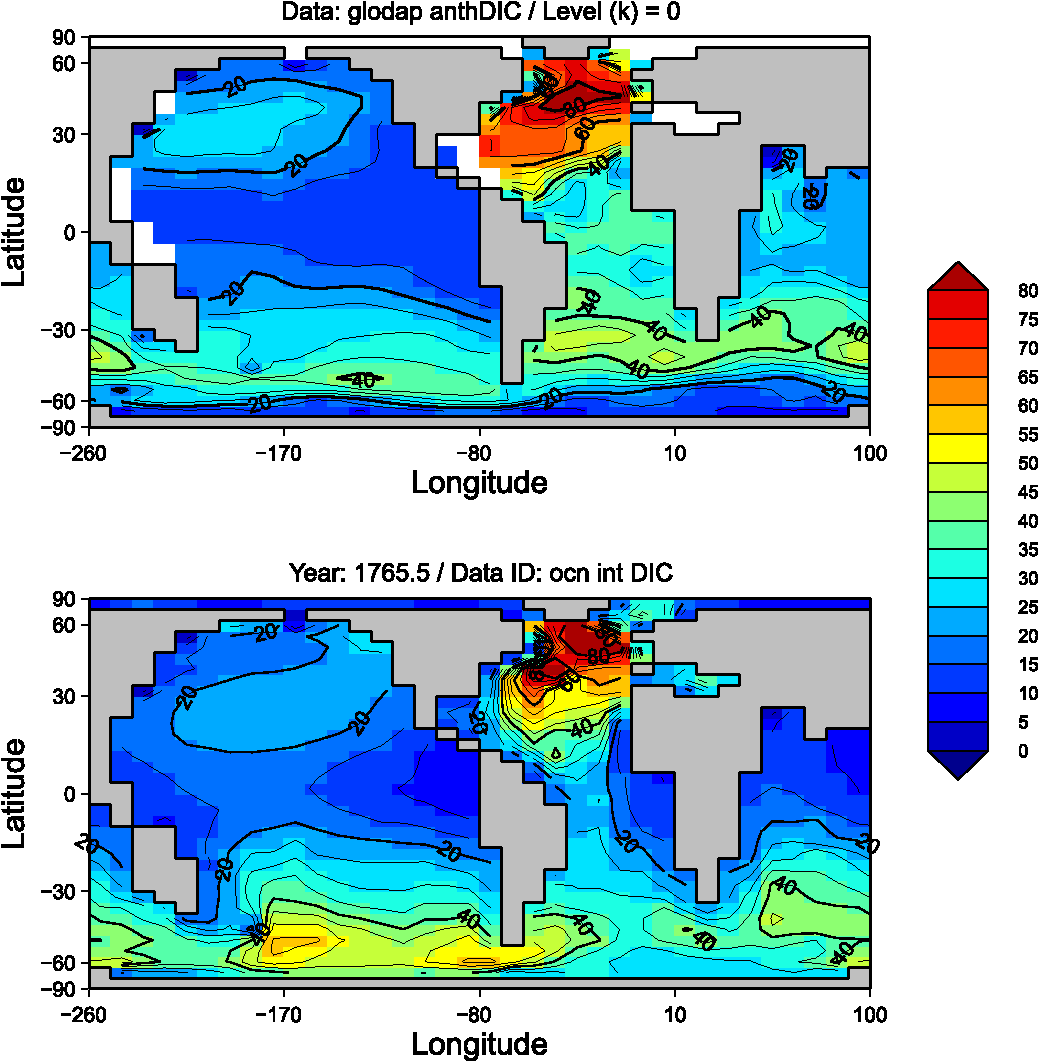
\includegraphics[scale=0.5]{chx-co2uptake.pdf}
\end{center}
\vspace{-10pt}
\caption{Observed (top) \textit{vs.} Model (bottom) anthropogenic \(CO_{2}\) inventories.
Data and model water column integrals in units of mol \(CO_{2}\) m$^{-2}$ and are nominally with respect to year 1994.}
\label{fig:chx-co2uptake}
\end{figure}

%------------------------------------------------
\newpage
%------------------------------------------------

\subsection{Assessing future carbon emissions impacts}

\noindent Finally, and the closest to being slightly interesting: rather than applying highly idealized pulses  of \(CO_{2}\) emissions, the IPCC 'SRES' emissions scenarios\footnote{Note that the past few IPCC assessment reports have switched to 'using 'RCP's -- Representative Emissions Pathways, rather than the SRES emissions scenarios -- see later Section.}  can be used to make future projections with. An example forcing of this sort is provided and can be selected by changing the name of the forcing selection parameter (\textsf{\footnotesize bg\_par\_forcing\_name}) to any one of the following:

\vspace{1mm}
\begin{itemize}[noitemsep]
\item \textsf{\footnotesize pyyyyz.FpCO2\_Fp13CO2.A1\_AIM}
\item \textsf{\footnotesize pyyyyz.FpCO2\_Fp13CO2.A1G\_MINICAM}
\item \textsf{\footnotesize pyyyyz.FpCO2\_Fp13CO2.A1T\_MESSAGE}
\item \textsf{\footnotesize pyyyyz.FpCO2\_Fp13CO2.A2\_ASF}
\item \textsf{\footnotesize pyyyyz.FpCO2\_Fp13CO2.B1\_IMAGE}
\item \textsf{\footnotesize pyyyyz.FpCO2\_Fp13CO2.B2\_MESSAGE}
\end{itemize}
\vspace{1mm}

These are 'future' emissions scenarios, which all start at year 2010, and end at year 2100. They are derived from different socio-economic and future technological assumptions in making their future emissions projections.

\vspace{1mm}

Again, as these forcings have units of \(PgCyr^{-1}\) in the time-series files, you will need to add a scaling parameter to your \textit{user-config} file to turn units of \(PgCyr^{-1}\) into \(mol C yr^{-1}\):\footnote{For completeness also add in the specification of the isotopic composition of the carbon emissions -- refer back to the idealized experiments.}
\vspace{-2pt}\small\begin{verbatim}
bg_par_atm_force_scale_val_3=8.3333e+013
\end{verbatim}\normalsize\vspace{-2pt}

You will want to run your experiment starting from the end of the historical transient experiment you have just run rather than the original steady-state \textit{re-start}:\footnote{Note that the \textit{user-config} \textsf{\footnotesize LAB.5.1.future } is not provided for you – you will need to create this (or a file named whatever you like) by copying e.g., \textsf{\footnotesize LAB.5.1.emissions} and making the parameter changes described above (forcing specification parameter, emissions scaling parameter, and start year parameter).}
\vspace{-2pt}\small\begin{verbatim}
$ ./runcookie.sh cookie.CB.p_worjh2.rCARB LABS LAB.5.1.future 90 LAB.5.1.historical
\end{verbatim}\normalsize\vspace{-2pt}
and then set the start year to the year that the previous historical transient finished on (\(2010\)):
\vspace{-2pt}\small\begin{verbatim}
bg_par_misc_t_start=2010.0
\end{verbatim}\normalsize\vspace{-2pt}
and which will then give you an experiment finishing in year \(2100\).

%------------------------------------------------
\vspace{1mm} \noindent\rule{4cm}{0.1mm} \vspace{2mm}
%------------------------------------------------

\noindent You can also easily replace the details of the emissions with other SRES scenarios – simply find the year \textit{vs.} emissions rate information from the interweb\footnote{e.g., http://sres.ciesin.columbia.edu/final\_data.html} and edit or copy-and-paste the flux values for each decade into the file \footnotesize\textsf{biogem\_force\_flux\_atm\_pCO2\_sig.dat }\normalsize in the forcing directory.\textbf{ cookie} will then automatically interpolate between the decadal tie-points to give a continuous change in emissions. Now you are able to make a rather more realistic/plausible assessment of when and where potential ecological impacts (via assumed ocean chemistry criteria) might occur.

Try running (e.g. as jobs submitted to the cluster queue) some other actual or made up $CO_{2}$ emissions scenarios.

%------------------------------------------------
\newpage
%------------------------------------------------

\section{Further ideas}

Some further possibilities for investigations that build on the basic previous ones. 

%------------------------------------------------

\subsection{Assessing the importance of emissions rate}

By editing the flux magnitude and/or timing (i.e. the years that are assigned to the different forcing time-points) information of the idealized emissions forcings, you can control the \(CO_{2}\) emissions trajectory as well as the total of fossil fuel carbon burned. Explore some different assumptions about \(CO_{2}\) release rate \uline{but for the same total carbon emitted}, and note their differing impact on climate and ocean (carbonate) geochemistry.

\vspace{1mm}

More realistic and appropriate to our \textit{current} global experiment than a single rapid pulse is a lower rate (order of 10 or 20 \(PgCyr^{-1}\)) released over a longer interval (order of 100 years) as compared to a conceptual 1000 \(PgC\) near-instantaneous pulse. Because the experiments are getting longer to run in real time … remember to make appropriate use of the cluster queuing facility – i.e., think about whether you want to sit around starting at the screen for 15 minutes waiting for a new line of numbers appear – if not: submit to the cluster queue. For instance, one might try and address the question: “For a given total release of  fossil fuel \(CO_{2}\), is it safer to burn it slower?” The answer is maybe not completely obvious, as burning carbon resources slower will result in a small global impact, but perhaps one that persists for longer(??). You could conceive of an ensemble (related set) of model experiments, maybe one of 100 \(PgCyr^{-1}\) for 1 yr, one of 10 \(PgCyr^{-1}\) for 10 years, and one of 1 \(PgCyr^{-1}\) for 100 years, and run them all for e.g., 100 years.\footnote{These all represent rather unrealistically small total \(CO_{2}\) releases and you may want ot consider a total more like 1000 \(PgC\) or rather more. You may also want to think about more realistic shapes rather than pulses, such a some sort of ramp up and then down in the emissions rate (but for the same total emissions).} (As jobs submitted to the queue, all can be run simultaneously (with blank spaces between commands!).) (\uline{Don’t forget the control experiment}! (configured the same, except with 0 \(PgCyr^{-1}\) of emissions for 100 years).)

\vspace{1mm}

Note note that ideally you would create a new \textit{forcing} based on the original if you are editing the same original  \textit{forcing} and expecting to run different ones at the same time. Really, this is little more than you did in copying and renaming \textit{user-config} files in order to create new experiments ... except that now it involves copying and renaming entire directories in \textsf{\footnotesize genie-forcings}. Remember that the \textit{forcing} is specified by the directory name assigned to \texttt{bg\_par\_forcing\_name} (enclosed in \texttt{''}) and you will need to change this to match the name of your new \textit{forcing} directory.

%------------------------------------------------

\subsection{Determining thresholds of environmental impact}

There are various concerns about the impacts of continuing fossil fuel \(CO_{2}\) emissions and a number of proposed climatic (e.g., the \(1.5^{\circ} C \) paris protocol global warming limit often mentioned in policy documents) and ecological ‘tipping points’. You could assess the maximum allowable \(CO_{2}\) emissions to remain within particular global environmental limits in the model. For example:

\begin{itemize}[noitemsep]

\vspace{1mm}
\item What is the maximum total \(CO_{2}\) release that can be made without inducing aragonite under-saturation at the ocean surface anywhere (or any season – see Section 5.2.3 in the User Manual for seasonal time-slice data saving)? How important is the time-scale of emissions in determining this? For total emissions above this: where in the ocean does the surface first become under-saturated and what sort of (calcifying) organisms might be impacted there? How large would the emissions have to be in order to start to induce under-saturation with respect to aragonite at the surface in the tropics (home to socio-economically important reef systems)? These are questions that can be addressed with simple \(CO_{2}\) release experiments in ocean carbon cycle models and everyone seems to get a GRL paper out of it each and every time!

\vspace{1mm}
\item How important are \(CO_{2}\)-climate feedback in amplifying or diminishing future climate and ocean carbonate chemistry changes – e.g., is the same atmospheric p\(CO_{2}\) value reached with and without climate feedback (and surface warming) – if not, why? 

Hint: the solubility of \(CO_{2}\) in sea-water is a function of temperature and at higher temperatures, \(CO_{2}\) is less soluble. This means that with climate warming, \(CO_{2}\) solubility declines, less is taken up by the ocean and more is left in the atmosphere -- driving further heating in a \uline{positive feedback}.

\vspace{1mm}

All your \(CO_{2}\) emissions experiments to date have had this feedback enabled -- specified at the top of the \textit{user-config} file by:
\vspace{-2pt}\small\begin{verbatim}
# set climate feedback
ea_36=y
\end{verbatim}\normalsize\vspace{-2pt}

To quantify the role of the carbon-climate feedback, you need to run an identical emissions experiment, but with the feedback disabled:
\vspace{-2pt}\small\begin{verbatim}
# set climate feedback
ea_36=n
\end{verbatim}\normalsize\vspace{-2pt}

Note that you also to need to run a historical transient experiments with no carbon-climate feedback, if you are starting emissions experiments from the year 2010. i.e. you will have a set of future emissions experiments including the carbon-climate feedback that are run from a historical transient experiments that also includes carbon-climate feedback, vs. a set of future emissions experiments without the carbon-climate feedback that are run from a historical transient experiments that also \uline{does not include} carbon-climate feedback.

\vspace{1mm}

The importance of the feedback is simply the difference between the 2 sets of experiments, at the same year.

\vspace{1mm}
\item Also: How large a \(CO_{2}\) emission does it take to significantly ‘collapse’ the AMOC and over what time-scale? (Or alternatively: what is the atmospheric \(pCO_{2}\) threshold for AMOC collapse in \textbf{cookie}?)
\\ If the AMOC weakens or collapses … why in the absence of a prescribed freshwater perturbation does this happen? What physical process are at play in response to rapid \(CO_{2}\) release too the atmosphere that may act to reduce or shutdown deep-water formation in the ocean model? (Plotting appropriate ocean property anomalies between the \(CO_{2}\) release experiment and a control experiment might help.)
\\Related to a previous possible investigation -- does the rate of \(CO_{2}\) increase (for the same total release) matter? If so, why? What is happening in general to the structure and dynamics of the upper ocean when surface warming is very rapid?

\end{itemize}

\vspace{2mm}
\noindent Experiments could be hypothetical and consisting of \(CO_{2}\) pulses or ramps (or exponential) and run on directly from a pre-industrial spin-up, or more ‘realistic’ and run on from the end of a historical transient experiment (e.g., starting in year 2010).

%------------------------------------------------
\vspace{1mm} \noindent\rule{4cm}{0.1mm} \vspace{2mm}
%------------------------------------------------

%------------------------------------------------
\newpage
%------------------------------------------------

\noindent Also:

\begin{itemize}[noitemsep]

\vspace{1mm}
\item How much carbon can  be burned (and how quickly) such that atmospheric \(pCO_{2}\) does not increase any further and remains at some specific value (you might pick \(\times2\) or \(\times4\) preindustrial \(pCO_{2}\) (ca. 278 ppm))? This is difficult to determine well because to hold atmospheric \(pCO_{2}\)  constant, continuing emissions are required (as \(CO_{2}\) continues to be taken up by the ocean).
\vspace{1mm} 
\\One possible approach to tacking this, might be:
\vspace{1mm} 
\begin{enumerate}[noitemsep]
\item Run one or more (SRES) emissions scenarios and find the year at which your \(pCO_{2}\) threshold value is crossed. 
\item Re-run the same emissions experiment, but only for as many years as the threshold-crossing year you had identified, is reached. This will become your new \textit{re-start}.
\item Create a new experiment, with zero emissions, and run on from your new re-start. You should see atmospheric \(pCO_{2}\) start close to the value you reached at the end of the last experiment, but then decay away as the ocean continues to absorb carbon from the atmosphere. The decline in atmospheric \(pCO_{2}\) each year tells you something about the yearly emissions needed to keep atmospheric \(pCO_{2}\) constant.
\\An approximate rule-of-thump, is that \(1ppm\) in atmospheric \(pCO_{2}\) is equivalent to \(2 PgC\) (actually, a more exact conversion is \(1 ppm = 2.123 PgC\)). So you could calculate a yearly time-series of how much (in ppm) atmospheric \(pCO_{2}\) falls by each year ... convert this to PgC, and then create a new \textit{forcing}, with this as the annual emissions.
\item Create and run a new experiment, from the same \textit{re-start} experiment you created, and apply the new emissions forcing you created. See if atmospheric \(pCO_{2}\) is approximately maintained constant(?)  
\item If not sufficient constant to your satisfaction, you could also carry out a second iteration -- calculating from your latest experiment, the ppm change in \(pCO_{2}\) each year, converting to an emissions rate, and running a further experiment ...
\\Note that if you 'overhsoot' and \(pCO_{2}\) rises above the threshold value rather than falls below, you are allowed to have a \uline{negative} carbon emission to the atmosphere in your forcing.
\item The sum of the carbon emissions up to the threshold being reached, is your answer to how much more carbon can be burned and not cross that threshold ... but you will see that after that, further emissions are allowed without \(pCO_{2}\) exceeding the threshold. So the answer e.g. for year 2100 (or 2200) will be larger.
\end{enumerate}

\vspace{2mm}

There are automated ways provided in the model framework of  achieving this, and you can for instance simply tell \textbf{cookie}  to maintain a specific (or changing) value of atmospheric \(pCO_{2}\), and from this diagnose the emissions rate that was required. For instance, you'll see in the original \textit{re-start} \textit{user-config} for this chapter -- \textsf{\footnotesize cookie.CB.p\_worjh2.rCARB.SPIN} -- the \textit{forcing} used is 
\textsf{\footnotesize pyyyyz.RpCO2\_Rp13CO2}. If you go look in that forcing directory at:
\vspace{1mm}
\\\textsf{\footnotesize biogem\_force\_restore\_atm\_pCO2\_sig.dat} 
\vspace{1mm}
\\you will see a unit forcing. This is then scaled by the parameter \textsf{\footnotesize bg\_par\_atm\_force\_scale\_val\_3} to achieve a constant atmospheric \(pCO_{2}\) value of \(278 ppm\) --  \(0.278\times10^{-6} atm\). To specify a different \(pCO_{2}\) value, simple change the scaling factor (as per e.g., for the flux forcing).

The equivalent carbon emissions required to do this, are diagnosed and provided as a \textit{time-series} output (in units of \(mol C yr^{-1}\)) in file: \\\textsf{\footnotesize biogem\_series\_diag\_misc\_specified\_forcing\_pCO2.res}

\vspace{1mm}
\item Similarly -- how much more carbon can be burned but still keep global mean surface air temperature from rising beyond the 'Paris' limit of \(2^{\circ}C\) (as compared to preindustrial)?
\\This is also difficult to determine well because there are significant climate lags in the system with warming continuing even if atmospheric \(pCO_{2}\) was held constant.
\\Trial-and error would be one approach ...

\end{itemize}

%------------------------------------------------

\subsection{Future atmospheric CO$_{2}$ concentration pathways ('RCPs')}

The more recent/current incarnation of IPCC future scenarios revolves not around  making projections of future greenhouse gas emissions rates, but rather future greenhouse gas concentration pathways. (The reasoning is partly to cut out the differences in carbon cycle feedback between models, where for the same unit \(CO_{2}\) release, different climate/Earth system models might project a different atmospheric \(CO_{2}\) concentration and hence climate change (in addition to differences between models in climate sensitivity).) In \textbf{cookie}, these work pretty well much like in the historical forcing scenario, where the observed change in atmospheric \(CO_{2}\) concentration in the atmosphere with time, is prescribed and the model 'forced' to conform to this trajectory.

\vspace{1mm}

A series of RCP scenarios for how atmospheric \(CO_{2}\) concentrations may evolve with time are provided. Each actually starts at year 1765 and hence incorporates the historical transient. They can hence be used with an experiment starting at 1765 and \textit{re-starting} from a steady-state preindustrial \textit{spin-up}. Or they can be jumped into at ay point, and e.g. experiments started at year 2010, when only the year 2010 onwards part of the \(CO_{2}\) restoring \textit{forcing} is utilized. The RCP \textit{forcings} currently provided are:

\vspace{1mm}
\begin{itemize}[noitemsep]
\setlength{\itemindent}{.2in}
\item \textsf{\footnotesize pyyyyz.RpCO2\_Rp13CO2.RCP3PD}
\item \textsf{\footnotesize pyyyyz.RpCO2\_Rp13CO2.RCP4p5}
\item \textsf{\footnotesize pyyyyz.RpCO2\_Rp13CO2.RCP6p0}
\item \textsf{\footnotesize pyyyyz.RpCO2\_Rp13CO2.RCP8p5}
\end{itemize}
\vspace{2mm}
and can be selected simply by changing the name of the forcing in the \textit{user-confi}g, e.g.:
\vspace{-2pt}\small\begin{verbatim}
bg_par_forcing_name=’pyyyyz.RpCO2_Rp13CO2.RCP8p5'
\end{verbatim}\normalsize\vspace{-2pt}
\noindent which would select the RCP8.5 scenario.

\vspace{1mm}

\noindent \uline{NOTE}: ensure that
the scaling parameters are either commented out, e.g.:
\vspace{-2pt}\small\begin{verbatim}
#bg_par_atm_force_scale_val_3=8.3333e+013
#bg_par_atm_force_scale_val_4=-27.0
\end{verbatim}\normalsize\vspace{-2pt}
\noindent or simply deleted in their entirety (because the RCP forcing contains the actual values/correct units and you do not need to modify them any further).

\vspace{1mm}

The equivalent carbon emissions required to follow these concentration pathways are diagnosed by \textbf{cookie} and provided as a \textit{time-series} output (in units of \(mol C yr^{-1}\)) in file: 
\vspace{1mm}
\\\textsf{\footnotesize biogem\_series\_diag\_misc\_specified\_forcing\_pCO2.res}

%------------------------------------------------
\newpage
%------------------------------------------------

\subsection{Isotopic tracing of fossil fuel CO$_{2}$ uptake}

\noindent The  experiments on fossil fuel \(CO_{2}\) emissions to the atmosphere include an assumed isotopic composition of the emitted carbon. For any of the carbon emissions experiments you have run (including the historical transient) -- explore in the 3D output how the  isotopic composition of fossil fuel carbon is propagated from the atmosphere into the ocean and  through the ocean via its large-scale circulation. The variable you want to plot is: \textsf{\footnotesize ocn\_DIC\_13C}\footnote{Also calculated and saved are the isotopic compositions of the 3 different aqueous carbonate chemsitry components -- \textsf{\footnotesize carb\_d13C\_CO2}, \textsf{\footnotesize carb\_d13C\_CO32}, and \textsf{\footnotesize carb\_d13C\_HCO3}.}. In this, it is helpful to also take a control experiment (you did run one, right ... ?) and create a difference map to better visualize how the \(\delta^{13}C\) patterns in the ocean evolve through time.

%------------------------------------------------
\vspace{1mm} \noindent\rule{4cm}{0.1mm} \vspace{2mm}
%------------------------------------------------

\noindent By default, fossil fuel carbon is tagged with a mean fossil fuel isotopic signature of \(-27\)\permille. This in set by the parameter:
\vspace{-1mm}\small\begin{verbatim}
bg_par_atm_force_scale_val_4=-27.0
\end{verbatim}\normalsize\vspace{-1mm}
which scales the value of \(1.0\) specified in the file \textsf{\footnotesize biogem\_force\_flux\_atm\_pCO2\_13C\_sig.dat} in the \textit{forcing} directory, which in the previous fossil fuel release experiments was the \textsf{\footnotesize genie-forcing} sub-directory: \textsf{\footnotesize pyyyyz.FpCO2\_Fp13CO2}

\vspace{1mm}

To create a more pronounced 'tag' (or tracer) of fossil fuel carbon, you could, for instance, make the assumed value of the \(CO_{2}\) more negative, e.g. \(-60\)\permille would be the signature of methane (natural gas). You could also push the value even more negative and consider it an idealized numerical tracer of fossil fuel carbon (note that the lowest value you are allowed to set is \(-999\)\permille).

%------------------------------------------------
\vspace{1mm} \noindent\rule{4cm}{0.1mm} \vspace{2mm}
%------------------------------------------------

\noindent (Also see: 12.2.1)

%----------------------------------------------------------------------------------------
%----------------------------------------------------------------------------------------
%----------------------------------------------------------------------------------------
%       CHAPTER 6
%----------------------------------------------------------------------------------------

\cleardoublepage

\chapterimage{oceanacidification.png} % Chapter heading image

\chapter{Fossil fuel CO$_{2}$ and 'ocean acidification'}

\hfill \break

%------------------------------------------------
\newpage
%------------------------------------------------

\section{(none)}

%----------------------------------------------------------------------------------------
%----------------------------------------------------------------------------------------
%%----------------------------------------------------------------------------------------
%       CHAPTER 6
%----------------------------------------------------------------------------------------

\cleardoublepage

\chapterimage{oceanacidification.png} % Chapter heading image

\chapter{Fossil fuel CO$_{2}$ and 'ocean acidification'}\label{ch:fossil-fuel-co2}

\hfill \break

%------------------------------------------------
\newpage
%------------------------------------------------

\section*{Readme}

You will need to download a new \textit{restart} file prior to embarking on the experiments. This pre-industrial spin-up includes a basic ocean (-atmosphere) carbon cycle plus various diagnostic anthropogenic tracers, following \textit{Cao et al.} [2009].

\vspace{2mm}

\noindent To fetch this: change to the \textsf{\footnotesize cgenie\_output} directory, and type ... or perhaps, \textbf{copy!} (\uline{but onto all one line}):
\vspace{-2mm}
\begin{verbatim}
$ wget --no-check-certificate 
   http://www.seao2.info/cgenie_output/muffin.CB.p_worjh2.rCARB.SPIN.tar.gz
\end{verbatim}
\vspace{-2mm}

\noindent Extract the contents of this archive by typing:
\vspace{-2mm}
\begin{verbatim}
$ tar xfzv muffin.CB.p_worjh2.rCARB.SPIN.tar.gz
\end{verbatim}
\vspace{-2mm}
\noindent (and then change directory back to \textsf{\footnotesize genie-main} to run the model)

%------------------------------------------------
\newpage
%------------------------------------------------

\section{Exploring the consequences of fossil fuel CO$_{2}$ emissions}

For the next experiment(s) you can chuck \(CO_{2}\) into the atmosphere, just for the hell of it. As much as you want! Apparently, humans are actually doing this now. Imagine that!

\vspace{1mm}

A new \textit{user-config} for \textbf{muffin} -- \footnotesize\textsf{ch06.CO2emissions }\normalsize -- is provided and configured with climate being responsive to any changes in atmospheric \(CO_{2}\) (i.e., it takes account of \(CO_{2}\)-climate feedback). 
\vspace{1mm}
The setting (near the top of the \textit{user-config} file) that does this is:
\vspace{-2pt}\small\begin{verbatim}
# set CO2-climate feedback
ea_36=y
\end{verbatim}\normalsize\vspace{-2pt}
\noindent Disabling this results in climate being fixed at a radiative forcing equivalent to $\times 1 CO_{2}$ (278 ppm).

In this \textit{user-config}, a release of \(CO_{2}\) to the atmosphere is prescribed, which by default is set to a value of just \(1\:PgC\) (cf. current emissions are ca. \(10\:PgC\:yr^{-1}\)) and over an interval of just a single year. (Releasing \(CO_{2}\) just over a single year is obviously rather unrealistic and many impacts will decay away rapidly, but represents a useful idealized experiment for assessing the time-scale(s) of fossil fuel \(CO_{2}\) uptake by the ocean.)

\vspace{1mm}
Additional (netCDF) output has also been prescribed, via the \textit{user-config} parameter setting: \texttt{bg\_par\_data\_save\_level=10} (see Section 14.4) so that more information relevant to assessing ocean acidification is saved.

%------------------------------------------------
\vspace{1mm}
\noindent\rule{4cm}{0.1mm}
\vspace{2mm}
%------------------------------------------------

\noindent First, run the experiment for e.g., 10 (or more if you like) years, starting from the pre-industrial \textit{re-start} experiment \textsf{\footnotesize muffin.CB.p\_worjh2.rCARB.SPIN}, i.e.:
\begin{verbatim}
$ ./runmuffin.sh muffin.CB.p_worjh2.rCARB LABS
   ch06.CO2emissions 10 muffin.CB.p_worjh2.rCARB.SPIN
\end{verbatim}

\noindent As for what model results variables to consider … think about the climate change and ocean acidification literature and which environmental (physical and geochemical) properties are considered either critical for ecosystems or are simply helpful and/or illustrative. Refer to Section 14.6.2 for a summary of some of the key ocean acidification (and other) variables that may be saved by the model\footnote{(depending on specific data saving configuration)}.
In the 3-D netCDF \textit{time-slice} file remember, for instance, that ocean surface waters in which aragonite becomes under-saturated (OHMEGA < 1.0) is regarded as a critical threshold for organisms making aragonite shells and skeletons and spells TROUBLE for some poor calcifying marine organism somewhere. (Temperature is also highly relevant to marine ecosystems under future global change.) Note that the calcification response is encoded in the model and described in \textit{Ridgwell et al.} [2007a,b] and may or may not reflect the Real World.

For climate change ... the variables of particular interest should be obvious. Remember that there are both \textit{time-series} outputs, as well as  2D and 3D fields, any or all of which might be  helpful for elucidating impacts.

%------------------------------------------------
\newpage
%------------------------------------------------

\subsection{Idealized emissions forcing}

\noindent You can easily modify the experimental design to release more/less \(CO_{2}\) very much as you did for the red dye tracer. In the \textit{user-config} file, the line:
\vspace{-2pt}\small\begin{verbatim}
bg_par_atm_force_scale_val_3=8.3333e+013
\end{verbatim}\normalsize\vspace{-2pt}
scales the time-history of the  \(CO_{2}\) flux, given in the forcing file:

\vspace{2pt}
\noindent \footnotesize\textsf{biogem\_force\_flux\_atm\_pCO2\_sig.dat}\normalsize
\vspace{2pt}

\noindent ... which can be found in the directory:

\vspace{2pt}
\noindent \footnotesize\textsf{cgenie.muffin/genie\_forcings/pyyyyz.FpCO2\_Fp13CO2}\normalsize
\vspace{2pt}

\vspace{2pt}
\noindent The format of this file is:
\vspace{-2pt}\small\begin{verbatim}
-START-OF-DATA-
     0.0  1.0
     1.0  1.0
     1.0  0.0
999999.9  0.0
-END-OF-DATA-
\end{verbatim}\normalsize\vspace{-2pt}

\noindent and defines an emission of \(1 mol C\) (carbon) per year over the first year (year 1.0) of the model experiment (between year \texttt{0.0} and \texttt{1.0}), but which in the example \textit{user-config} is then scaled by a value of \(8.333\times10^{13}\) (by the parameter \texttt{bg\_par\_atm\_force\_scale\_val\_3}) to give a total of \(1 PgC yr^{-1}\). (Year 999999.9 has no special meaning and is simply just waaaaay into the future …)

\vspace{1mm}

Pause … and note briefly how the final \(CO_{2}\) flux is arrived at. \textbf{muffin} calculates it by multiplying the value in the forcing file (1.0) by a modifying parameter in the \textit{user-config} file (\texttt{8.3333e+13}). The total flux is hence: \(1.0 \times 8.333\times10^{13} = 8.333\times10^{13} mol CO_{2} yr^{-1}\). If you set both values as \texttt{1.0}, you’d get very little carbon released (a single mol!). If you screw up and multiply \texttt{8.3333e+013} and \texttt{8.3333e+013} together as the total flux ... you’ll soon know it as you cook the Earth … But it does not matter which parameter has value \texttt{1.0} and which scales the units (\texttt{8.3333e+013}). For now, it is simply more convenient to be able to edit the \textit{forcing} file with 'simple' numbers (and leave the large numbers and units conversion in the \textit{user-config} file).

Together, the scaling and forcing value gives a \(CO_{2}\) release of \(1 PgC yr^{-1}\) for just a single year compared to current emissions are about \(10 PgC yr^{-1}\). So, do not expect anything exciting if all you emit to the atmosphere is a single measly \(1 PgC\) (over 1 year).

(The parameter: \texttt{\small bg\_par\_atm\_force\_scale\_val\_4=-27.0} specifies the carbon isotopic composition of fossil fuel carbon and can be ignored for now.)

%------------------------------------------------
\vspace{1mm}
\noindent\rule{4cm}{0.1mm}
\vspace{2mm}
%------------------------------------------------

\noindent Because ‘accidents can happen’ and the global environmental changes induced by the massive fossil fuel \(CO_{2}\) release can obscure mistakes made in the experiment configuration (parameter values) and/or the \textit{re-start} used, you are strongly advised to first (or in parallel, as a job submitted to the cluster – refer to Lesson Zero to remind yourself of the commend line syntax needed for this) --  and \uline{run a control experiment}:
\vspace{-2pt}\small\begin{verbatim}
$ ./runmuffin.sh muffin.CB.p_worjh2.rCARB LABS ch06.CONTROL 10
   muffin.CB.p_worjh2.rCARB.SPIN
\end{verbatim}\normalsize\vspace{-2pt}
Here – the \textit{user-config} defining the control experiment (\texttt{ch06.CONTROL}) is \uline{identical} to that for the actual experiment itself (\textsf{\footnotesize ch06.CO2emissions}) \uline{with the exception of} the scaling of the \(CO_{2}\) emissions, that is set to zero. i.e.:
\vspace{-0pt}\small\begin{verbatim}
bg_par_atm_force_scale_val_3=8.3333e+013
\end{verbatim}\normalsize\vspace{-2pt}

Note that it is left completely up to you to create (i.e. copy and edit!) the experiment configuration file \textsf{\footnotesize ch06.CONTROL} ...

\vspace{1mm}

If everything is OK with the control experiment, atmospheric \(CO_{2}\) (and climate) following on from the \textit{re-start} should be stable and there should be little (or no) drift in any of the output variables (because the \textit{spin-up} you are re-starting from should have been run to an equilibrium state and you have not changed anything in the control experiment, right?).

\vspace{1mm}

It is good practice (i.e., always do it!) to \uline{always run a control experiment} for each different type of experiment – e.g., you only need to run one control experiment for a set \(CO_{2}\) emissions experiments differing only in total carbon release of the time-history of that release.

When you have run both the real and control experiment, compare the results. View (or plot) both relevant \textit{time-series} output, and create anomaly maps of key \textit{time-slice} variables in \textbf{Panoply} or \textbf{MATLAB}, using a corresponding \textit{time-slice} from the control experiment to create the experiment anomaly with.

\vspace{1mm}
\noindent\rule{4cm}{0.1mm}
\vspace{2mm}

\noindent OK. You might want to run something a little more exciting now. For instance, rather than
\vspace{-2pt}\small\begin{verbatim}
-START-OF-DATA-
     0.0  1.0
     1.0  1.0
     1.0  0.0
999999.9  0.0
-END-OF-DATA-
\end{verbatim}\normalsize\vspace{-2pt}
you might have:
\vspace{-2pt}\small\begin{verbatim}
-START-OF-DATA-
     0.0  1000.0
     1.0  1000.0
     1.0     0.0
999999.9     0.0
-END-OF-DATA-
\end{verbatim}\normalsize\vspace{-2pt}
for a total of \(1000 PgC\) is released over a single year. Now you should see some policy-relevant impacts occur :o)

\noindent (Again, contrast control and experiment results to quantify/visualize the impacts of the \(CO_{2}\) release.)

%------------------------------------------------
\vspace{1mm}
\noindent\rule{4cm}{0.1mm}
\vspace{2mm}
%------------------------------------------------

\noindent You can control the shape of the emissions profile as well as its magnitude. Between the start and end ‘tags’ in the text \textit{forcing} file, the data is arranged into 2 columns: the first contains a series of tie-points for defining the timing of changes in emissions, and the 2nd column contains flux information (units of \(PgC yr^{-1}\) when scaled by the parameter parameter \texttt{bg\_par\_atm\_force\_scale\_val\_3} in the \textit{user-config}). At each time-step of the model, the \(CO_{2}\) flux to be applied to the atmosphere is interpolated between these time points.

\vspace{1mm}

For instance, in the \textit{forcing} (directory) file \footnotesize\textsf{biogem\_force\_flux\_atm\_pCO2\_sig.dat}\normalsize, the purpose of:
\vspace{-2pt}\small\begin{verbatim}
     0.0  1.0
     1.0  1.0
     1.0  0.0
999999.9  0.0
\end{verbatim}\normalsize\vspace{-2pt}
is to specify a uniform flux of 1.0 (scaled to \(PgC yr^{-1}\)) over the first full year of the model run, followed by a sharp turn-off to zero flux at the end of first year (and remaining zero thereafter). To extend the period of emissions – for example:
\vspace{-2pt}\small\begin{verbatim}
     0.0  1.0
    10.0  1.0
    10.0  0.0
999999.9  0.0
\end{verbatim}\normalsize\vspace{-2pt}
would result in a uniform flux lasting 10 years with a sudden cut-off and zero thereafter (i.e., once scaled by the parameter in the \textit{user-config} – \(1 PgC yr^{-1}\) over 10 years – \(10 PgC\) total emissions). 

In contrast:
\vspace{-2pt}\small\begin{verbatim}
     0.0  0.0
    10.0  1.0
    10.0  0.0
999999.9  0.0
\end{verbatim}\normalsize\vspace{-2pt}
would result in a linear ramp, starting from zero at the start of year \(0.0,\) to \(1.0 PgC yr^{-1}\) at year \(10.0\) and then suddenly ceasing and remaining at zero for the remainder of the experiment (a total \(CO_{2}\) emission of \(1\times1.0\times0.5 = 5PgC\) over 10 years).

\vspace{1mm}

To ramp up (over 10 years), and then down again (over 10 years), you would specify:
\vspace{-2pt}\small\begin{verbatim}
     0.0  0.0
    10.0  1.0
    20.0  0.0
999999.9  0.0
\end{verbatim}\normalsize\vspace{-2pt}

Try making up a few 'shapes' (and hence different experiments), maybe for the same integrated/total emissions, explore the effect of different rates of rise/fall in the release rate. And/or for the same release rate and/or duration, explore the impact of different total emissions of \(CO_{2}\). Try and think in terms of hypotheses and formulate questions to guide your experimental design/configuration. (An alternative approach is to create random scenarios and in the analysis, fish for interesting patters that could lead to knowledge and/or specific questions to be tested further, but it is better to start off with a hypothesis in mind.)

Note that you can either edit and re-use the same \textit{forcing} directory and name, modifying the file \footnotesize\textsf{biogem\_force\_flux\_atm\_pCO2\_sig.dat }\normalsize each time but then losing an explicit record of how you might have set the emissions profile previously, or you can copy and rename the entire \textit{forcing} directory (and then edit \footnotesize\textsf{biogem\_force\_flux\_atm\_pCO2\_sig.dat }\normalsize). If you copy and rename the entire \textit{forcing} directory, in the \textit{user-config}, you then need to specify this new forcing (directory) name, e.g.:
\vspace{-2pt}\small\begin{verbatim}
# specify forcings
bg_par_forcing_name="pyyyyz.FpCO2_Fp13CO2.NEW"
\end{verbatim}\normalsize\vspace{-2pt}
if you, for instance, called your new \textit{forcing} directory (in \footnotesize\textsf{genie-forcings }\normalsize): \footnotesize\textsf{pyyyyz.FpCO2\_Fp13CO2.NEW}\normalsize.\footnote{Refer to the directory map in Figure 1.1. if in doubt here.}

\vspace{20pt}

%------------------------------------------------
\newpage
%------------------------------------------------

\subsection{Where has my carbon gone???}

In any of the emissions experiments you have tried out, in the time-series of atmospheric \(pCO_{2}\) (file: \textsf{\footnotesize biogem\_series\_atm\_pCO2.res}) you'll undoubtedly see atmospheric \(pCO_{2}\) initially rise, but then once the emissions cease, start decaying back down again. Where is it 'going'?

Well obviously the ocean. D'uh! (At least, this is true in this particularly configuration of \textbf{muffin} without a terrestrial biosphere.) A better question would be: 'where in the ocean has it gone?', and even better: 'why there?'.

In the 3D netCDF, the variable \textsf{\footnotesize ocn\_DIC} is the total dissolved carbon inorganic concentration (\(DIC\)). Open this up ... and by slicing horizontally (e.g. start at the surface, and then slice downwards), or vertically (up through the middle of the Atlantic would be a good latitude-vertical section to create), can you 'see' where the carbon (as \(DIC\)) is going? If not ... why not? Try making the same data sections from the same year of the control experiment. \(DIC\) is everywhere in the ocean in the control, with a highly spatially variable distribution. It could be then that the carbon taken up from the atmosphere in your experiment, simply overprints too small a pattern of (fossil fuel \(DIC\)) to tell background + fossil fuel from just background. (A similar situation arose when looking for the surface temperature impact of a weakening AMOC.)

To resolve this, create difference maps of a slice (lon-lat, or lat-depth) from your experiment at time \(t\) minus the control, also at time \(t\). Now re-evaluate whether you can tell where the fossil fuel \(CO_{2}\) is going. Why (there)? (We'll also consider this question in the next exercise.)

%------------------------------------------------
\vspace{1mm}
\noindent\rule{4cm}{0.1mm}
\vspace{2mm}
%------------------------------------------------

\noindent What about the other carbonate system parameters? Can you track identify patterns of uptake and ocean circulation transport. For instance \(CO_{2(aq)}\)? What about \(CO^{2-}_{3}\) (before looking, and remembering your basic carbonate chemistry, what would you expect)? (\(HCO^{2-}_{3}\) should primarily track \(DIC\).)

Are there any other carbonate system impacts you can discern? Some fields to consider might include:

\vspace{1mm}
\begin{itemize}[noitemsep]
\item \(pH\) -- variable \textsf{\footnotesize misc\_pH} 
\\(There is also a field for the hydrogen ion concentration if you really want to see it.)
\item Calcite saturation state (\(\Omega_{(cal)}\)) -- variable \textsf{\footnotesize carb\_ohm\_cal}
\item Aragonite saturation state (\(\Omega_{(arg)}\)) -- variable \textsf{\footnotesize carb\_ohm\_arg} 
\end{itemize}

\vspace{1mm}
\noindent\rule{4cm}{0.1mm}
\vspace{2mm}

\noindent In looking at the different fields and based on your reading of the literature (you did read the background papers, right ... ?), think about what organisms live where and what environmental (carbonate system) variables might affect them (or their prey).

%------------------------------------------------
\newpage
%------------------------------------------------

\subsection{Historical (real-world!) emissions forcing}

Historical and future (e.g. IPCC 'SRES') emissions scenarios can  be prescribed explicitly and simply in \textbf{muffin}. An example is given as \textit{user-config} file: \textsf{\footnotesize ch06.historical}. In this, a historical emissions forcing (technically: a prescribed concentration profile of \(pCO_{2}\) (and other anthropogenic gases) is specified by the \textit{forcing}:
\vspace{-2pt}\small\begin{verbatim}
bg_par_forcing_name=’worjh2.historical2010’
\end{verbatim}\normalsize\vspace{-2pt}
In contrast to before, no additional scaling is needed because the forcing specification directly follows the observed change in atmospheric concentration with time (in units of atm \(CO_{2}\)).

\vspace{1mm}

Note that an additional line appears in the \textit{user-config}. This is because the historical \(pCO_{2}\) transient starts in the 1700s (for which a nominal date of 1765 is often used) rather than year zero. To start \textbf{muffin} counting from year 1765 rather than year zero, a start year parameter value is specified:
\vspace{-2pt}\small\begin{verbatim}
bg_par_misc_t_start=1765.0
\end{verbatim}\normalsize\vspace{-2pt}
It is also convenient to specify a set of points in time at which data is saved that are consistent with the historical period. In the example \textit{user-config}, the addition of the parameter settings:
\vspace{-2pt}\small\begin{verbatim}
bg_par_infile_slice_name=’save_timeslice_historicalfuture.dat’
bg_par_infile_sig_name=’save_timeseries_historicalfuture.dat’
\end{verbatim}\normalsize\vspace{-2pt}
specifies a series of time points at which data is saved that aligns with historically relevant years.

Try viewing the contents of these (text) files:
\vspace{2pt}
\\ \footnotesize\textsf{save\_timeslice\_historicalfuture.dat }\normalsize
\\ \footnotesize\textsf{save\_timeseries\_historicalfuture.dat }\normalsize
\vspace{2pt}
\\which can be found in the directory: \footnotesize\textsf{genie-biogem/data/input }\normalsize, to get a sense of how frequently the data will be saved, and how this differs from the default settings, which are defined in the files:
\vspace{2pt}
\\ \footnotesize\textsf{save\_timeseries.dat }\normalsize
\\ \footnotesize\textsf{save\_timeslice.dat }\normalsize
\vspace{2pt}

%------------------------------------------------
\vspace{1mm}
\noindent\rule{4cm}{0.1mm}
\vspace{2mm}
%------------------------------------------------

\noindent Running a transient historically-forced experiment looks like this (\uline{all one line}!):
\vspace{-2pt}\small\begin{verbatim}
$ ./runmuffin.sh muffin.CB.p_worjh2.rCARB LABS ch06.historical 245
   muffin.CB.p_worjh2.rCARB.SPIN
\end{verbatim}\normalsize\vspace{-2pt}
The \texttt{245} parameter value for experiment duration arises on the basis of the start year being \(1765\) (as specified by \texttt{\small bg\_par\_misc\_t\_start=1765.0}) and to give an experiment end at year \(2100\).

\vspace{1mm}

Note that from year 1765 onward, changes in atmospheric \(CO_{2}\) only rise very s l o w l y initially. Don't expect to see anything happen in 10 seconds flat because relatively few people and countries in the 1800s could be bothered to burn much more than a little local coal. You could potentially start your experiment at year 1850, changing the value of \texttt{\small bg\_par\_misc\_t\_start} and specifying shorter experiment duration (\(150\) years) if you are desperate for the End of the World to come.

Don’t forget: you could submit this experiment to the cluster and do more (idealized emissions) ‘playing’ which it runs.

%\vspace{1mm}
%\noindent\rule{4cm}{0.1mm}
%\vspace{2mm}

\noindent Given that there is observationally-based information on the distribution of anthropogenic \(CO_{2}\) taken up by the ocean (e.g., \textit{Sabine et al.} [2004]) ... and you are running a historical transient experiment with the model driven by observed increases in atmospheric p\(CO_{2}\) ... you are in a position to critically evaluate the models ability (or lack of) to represent the future-critical process of oceanic fossil fuel \(CO_{2}\) uptake and transport by large scale ocean circulation.

\vspace{1mm}

In the 2D \textbf{netCDF} output, there is a variable for the water column integrated inventory of DIC – equivalent to the Sabine map except you will need to subtract the preindustrial background of DIC first, i.e., to create a DIC anomaly map representing only the added fossil fuel \(CO_{2}\) component of ocean DIC. The data in the Sabine paper clusters around 1994. A \textit{time-slice} centered on this year (1994.5) has been configured in the model exactly for this purpose. Your baseline state can either be from prior to \(CO_{2}\) emissions commencing at any significant rate (e.g., 1750.5) or (better), from a control experiment. Note that similar comparisons could be (and are regularly) made with other tracers such as CFCs, which provide additional insights into the patterns and time-scales of trace gas update and ocean circulation. (See: \textit{Cao et al.} [2009])

\vspace{1mm}

Observational data, re-gridded to the \textbf{muffin} grid and in netCDF format can be downloaded from: \href{http://www.seao2.org/mymuffin.html}{http://www.seao2.org/mymuffin.html} (and under the ‘got data?’ box on the left). You could for instance, compare horizontal or vertical slices (3D netCDF) and create difference (anomaly) maps. Somewhat more representative of the entire ocean is to compare (or calculate difference maps) of zonal average profiles. Unfortunately, the observations are not in the form of water column integrals and hence you cannot create difference maps of model as per the \textit{Sabine} paper … unless you use the 3D \textbf{BIOGEM} \textbf{MATLAB} plotting scripts. Examples of \textbf{MATLAB} plotting of the model \textit{vs.} observed anthropogenic anomaly are shown in Figure \ref{fig:chx-co2uptake}.

\vspace{2mm}

\begin{figure}[ht]
\begin{center}
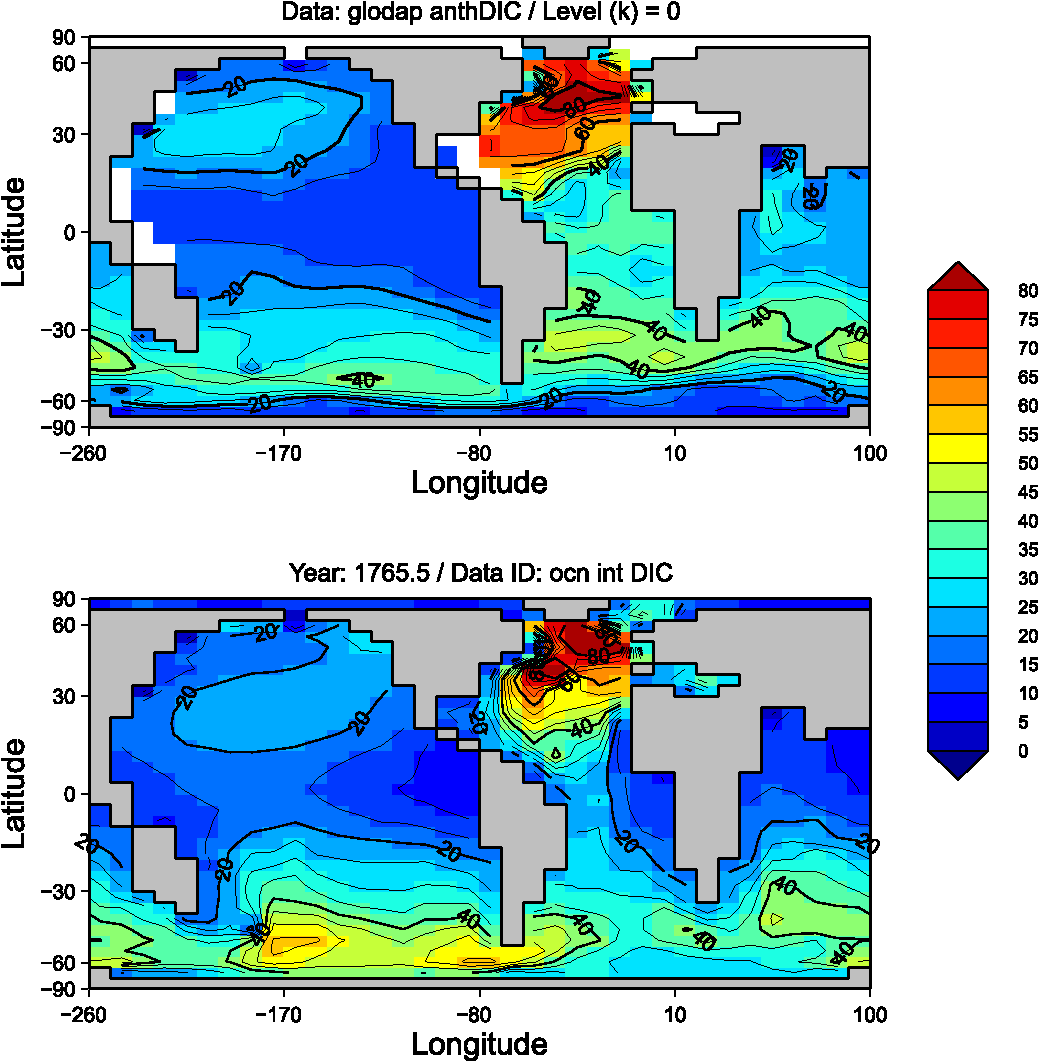
\includegraphics[scale=0.5]{chx-co2uptake.pdf}
\end{center}
\vspace{-10pt}
\caption{Observed (top) \textit{vs.} Model (bottom) anthropogenic \(CO_{2}\) inventories.
Data and model water column integrals in units of mol \(CO_{2}\) m$^{-2}$ and are nominally with respect to year 1994.}
\label{fig:chx-co2uptake}
\end{figure}

%------------------------------------------------
\newpage
%------------------------------------------------

\subsection{Assessing future carbon emissions impacts}

\noindent Finally, and the closest to being slightly interesting: rather than applying highly idealized pulses  of \(CO_{2}\) emissions, the IPCC 'SRES' emissions scenarios can be used to make future projections with. An example forcing of this sort is provided and can be selected by changing the name of the forcing selection parameter (\texttt{bg\_par\_forcing\_name}) to any one of the following:

\vspace{1mm}
\begin{itemize}[noitemsep]
\item \textsf{\footnotesize pyyyyz.FpCO2\_Fp13CO2.A1\_AIM}
\item \textsf{\footnotesize pyyyyz.FpCO2\_Fp13CO2.A1G\_MINICAM}
\item \textsf{\footnotesize pyyyyz.FpCO2\_Fp13CO2.A1T\_MESSAGE}
\item \textsf{\footnotesize pyyyyz.FpCO2\_Fp13CO2.A2\_ASF}
\item \textsf{\footnotesize pyyyyz.FpCO2\_Fp13CO2.B1\_IMAGE}
\item \textsf{\footnotesize pyyyyz.FpCO2\_Fp13CO2.B2\_MESSAGE}
\end{itemize}
\vspace{1mm}

These are 'future' emissions scenarios, which all start at year 2010, and end at year 2100. They are derived from different socio-economic and future technological assumptions in making their future emissions projections.

\vspace{1mm}

Again, as these forcings have units of \(PgCyr^{-1}\) in the time-series files, you will need to add a scaling parameter to your \textit{user-config} file to turn units of \(PgCyr^{-1}\) into \(mol C yr^{-1}\):\footnote{For completeness also add in the specification of the isotopic composition of the carbon emissions -- refer back to the idealized experiments.}
\vspace{-2pt}\small\begin{verbatim}
bg_par_atm_force_scale_val_3=8.3333e+013
\end{verbatim}\normalsize\vspace{-2pt}

You will want to run your experiment starting from the end of the historical transient experiment you have just run rather than the original steady-state \textit{re-start}:\footnote{Note that the \textit{user-config} \footnotesize\textsf{ch06.future }\normalsize is not provided for you – you will need to create this (or a file named whatever you like) by copying e.g., \footnotesize\textsf{ch06.EXAMPLE }\normalsize and making the parameter changes described above (forcing specification parameter, emissions scaling parameter, and start year parameter).}
\vspace{-2pt}\small\begin{verbatim}
$ ./runmuffin.sh muffin.CB.p_worjh2.rCARB LABS ch06.future 90 ch06.historical
\end{verbatim}\normalsize\vspace{-2pt}
and then set the start year to the year that the previous historical transient finished on (\(2010\)):
\vspace{-2pt}\small\begin{verbatim}
bg_par_misc_t_start=2010.0
\end{verbatim}\normalsize\vspace{-2pt}
and which will then give you an experiment finishing in year \(2100\).

%------------------------------------------------
\vspace{1mm}
\noindent\rule{4cm}{0.1mm}
\vspace{2mm}
%------------------------------------------------

\noindent You can also easily replace the details of the emissions with other SRES scenarios – simply find the year \textit{vs.} emissions rate information from the interweb\footnote{e.g., http://sres.ciesin.columbia.edu/final\_data.html} and edit or copy-and-paste the flux values for each decade into the file \footnotesize\textsf{biogem\_force\_flux\_atm\_pCO2\_sig.dat }\normalsize in the forcing directory.\textbf{ muffin} will then automatically interpolate between the decadal tie-points to give a continuous change in emissions. Now you are able to make a rather more realistic/plausible assessment of when and where potential ecological impacts (via assumed ocean chemistry criteria) might occur.

Try running (e.g. as jobs submitted to the cluster queue) some other actual or made up SRES emissions scenarios.

(Note that the past few IPCC assessment reports have switched to 'using 'RCP's -- Representative Emissions Pathways, rather than the SRES emissions scenarios -- see later Section.)

%------------------------------------------------
\newpage
%------------------------------------------------

\section{Further ideas}

Some further possibilities for investigations that build on the basic previous ones. 

%------------------------------------------------

\subsection{Assessing the importance of emissions rate}

By editing the flux magnitude and/or timing (i.e. the years that are assigned to the different forcing time-points) information of the idealized emissions forcings, you can control the \(CO_{2}\) emissions trajectory as well as the total of fossil fuel carbon burned. Explore some different assumptions about \(CO_{2}\) release rate \uline{but for the same total carbon emitted}, and note their differing impact on climate and ocean (carbonate) geochemistry.

\vspace{1mm}

More realistic and appropriate to our \textit{current} global experiment than a single rapid pulse is a lower rate (order of 10 or 20 \(PgCyr^{-1}\)) released over a longer interval (order of 100 years) as compared to a conceptual 1000 \(PgC\) near-instantaneous pulse. Because the experiments are getting longer to run in real time … remember to make appropriate use of the cluster queuing facility – i.e., think about whether you want to sit around starting at the screen for 15 minutes waiting for a new line of numbers appear – if not: submit to the cluster queue. For instance, one might try and address the question: “For a given total release of  fossil fuel \(CO_{2}\), is it safer to burn it slower?” The answer is maybe not completely obvious, as burning carbon resources slower will result in a small global impact, but perhaps one that persists for longer(??). You could conceive of an ensemble (related set) of model experiments, maybe one of 100 \(PgCyr^{-1}\) for 1 yr, one of 10 \(PgCyr^{-1}\) for 10 years, and one of 1 \(PgCyr^{-1}\) for 100 years, and run them all for e.g., 100 years.\footnote{These all represent rather unrealistically small total \(CO_{2}\) releases and you may want ot consider a total more like 1000 \(PgC\) or rather more. You may also want to think about more realistic shapes rather than pulses, such a some sort of ramp up and then down in the emissions rate (but for the same total emissions).} (As jobs submitted to the queue, all can be run simultaneously (with blank spaces between commands!).) (\uline{Don’t forget the control experiment}! (configured the same, except with 0 \(PgCyr^{-1}\) of emissions for 100 years).)

\vspace{1mm}

Note note that ideally you would create a new \textit{forcing} based on the original if you are editing the same original  \textit{forcing} and expecting to run different ones at the same time. Really, this is little more than you did in copying and renaming \textit{user-config} files in order to create new experiments ... except that now it involves copying and renaming entire directories in \textsf{\footnotesize genie-forcings}. Remember that the \textit{forcing} is specified by the directory name assigned to \texttt{bg\_par\_forcing\_name} (enclosed in \texttt{''}) and you will need to change this to match the name of your new \textit{forcing} directory.

%------------------------------------------------

\subsection{Determining thresholds of environmental impact}

There are various concerns about the impacts of continuing fossil fuel \(CO_{2}\) emissions and a number of proposed climatic (e.g., the \(1.5^{\circ} C \) paris protocol global warming limit often mentioned in policy documents) and ecological ‘tipping points’. You could assess the maximum allowable \(CO_{2}\) emissions to remain within particular global environmental limits in the model. For example:

\begin{itemize}[noitemsep]

\vspace{1mm}
\item What is the maximum total \(CO_{2}\) release that can be made without inducing aragonite under-saturation at the ocean surface anywhere (or any season – see Section 5.2.3 in the User Manual for seasonal time-slice data saving)? How important is the time-scale of emissions in determining this? For total emissions above this: where in the ocean does the surface first become under-saturated and what sort of (calcifying) organisms might be impacted there? How large would the emissions have to be in order to start to induce under-saturation with respect to aragonite at the surface in the tropics (home to socio-economically important reef systems)? These are questions that can be addressed with simple \(CO_{2}\) release experiments in ocean carbon cycle models and everyone seems to get a GRL paper out of it each and every time!

\vspace{1mm}
\item How important are \(CO_{2}\)-climate feedback in amplifying or diminishing future climate and ocean carbonate chemistry changes – e.g., is the same atmospheric p\(CO_{2}\) value reached with and without climate feedback (and surface warming) – if not, why? 

Hint: the solubility of \(CO_{2}\) in sea-water is a function of temperature and at higher temperatures, \(CO_{2}\) is less soluble. This means that with climate warming, \(CO_{2}\) solubility declines, less is taken up by the ocean and more is left in the atmosphere -- driving further heating in a \uline{positive feedback}.

\vspace{1mm}

All your \(CO_{2}\) emissions experiments to date have had this feedback enabled -- specified at the top of the \textit{user-config} file by:
\vspace{-2pt}\small\begin{verbatim}
# set climate feedback
ea_36=y
\end{verbatim}\normalsize\vspace{-2pt}

To quantify the role of the carbon-climate feedback, you need to run an identical emissions experiment, but with the feedback disabled:
\vspace{-2pt}\small\begin{verbatim}
# set climate feedback
ea_36=n
\end{verbatim}\normalsize\vspace{-2pt}

Note that you also to need to run a historical transient experiments with no carbon-climate feedback, if you are starting emissions experiments from the year 2010. i.e. you will have a set of future emissions experiments including the carbon-climate feedback that are run from a historical transient experiments that also includes carbon-climate feedback, vs. a set of future emissions experiments without the carbon-climate feedback that are run from a historical transient experiments that also \uline{does not include} carbon-climate feedback.

\vspace{1mm}

The importance of the feedback is simply the difference between the 2 sets of experiments, at the same year.

\vspace{1mm}
\item Also: How large a \(CO_{2}\) emission does it take to significantly ‘collapse’ the AMOC and over what time-scale? (Or alternatively: what is the atmospheric \(pCO_{2}\) threshold for AMOC collapse in \textbf{muffin}?)
\\ If the AMOC weakens or collapses … why in the absence of a prescribed freshwater perturbation does this happen? What physical process are at play in response to rapid \(CO_{2}\) release too the atmosphere that may act to reduce or shutdown deep-water formation in the ocean model? (Plotting appropriate ocean property anomalies between the \(CO_{2}\) release experiment and a control experiment might help.)
\\Related to a previous possible investigation -- does the rate of \(CO_{2}\) increase (for the same total release) matter? If so, why? What is happening in general to the structure and dynamics of the upper ocean when surface warming is very rapid?

\end{itemize}

\vspace{2mm}
\noindent Experiments could be hypothetical and consisting of \(CO_{2}\) pulses or ramps (or exponential) and run on directly from a pre-industrial spin-up, or more ‘realistic’ and run on from the end of a historical transient experiment (e.g., starting in year 2010).

%------------------------------------------------
\vspace{1mm}
\noindent\rule{4cm}{0.1mm}
\vspace{2mm}
%------------------------------------------------

%------------------------------------------------
\newpage
%------------------------------------------------

\noindent Also:

\begin{itemize}[noitemsep]

\vspace{1mm}
\item How much carbon can  be burned (and how quickly) such that atmospheric \(pCO_{2}\) does not increase any further and remains at some specific value (you might pick \(\times2\) or \(\times4\) preindustrial \(pCO_{2}\) (ca. 278 ppm))? This is difficult to determine well because to hold atmospheric \(pCO_{2}\)  constant, continuing emissions are required (as \(CO_{2}\) continues to be taken up by the ocean).
\vspace{1mm} 
\\One possible approach to tacking this, might be:
\vspace{1mm} 
\begin{enumerate}[noitemsep]
\item Run one or more (SRES) emissions scenarios and find the year at which your \(pCO_{2}\) threshold value is crossed. 
\item Re-run the same emissions experiment, but only for as many years as the threshold-crossing year you had identified, is reached. This will become your new \textit{re-start}.
\item Create a new experiment, with zero emissions, and run on from your new re-start. You should see atmospheric \(pCO_{2}\) start close to the value you reached at the end of the last experiment, but then decay away as the ocean continues to absorb carbon from the atmosphere. The decline in atmospheric \(pCO_{2}\) each year tells you something about the yearly emissions needed to keep atmospheric \(pCO_{2}\) constant.
\\An approximate rule-of-thump, is that \(1ppm\) in atmospheric \(pCO_{2}\) is equivalent to \(2 PgC\) (actually, a more exact conversion is \(1 ppm = 2.123 PgC\)). So you could calculate a yearly time-series of how much (in ppm) atmospheric \(pCO_{2}\) falls by each year ... convert this to PgC, and then create a new \textit{forcing}, with this as the annual emissions.
\item Create and run a new experiment, from the same \textit{re-start} experiment you created, and apply the new emissions forcing you created. See if atmospheric \(pCO_{2}\) is approximately maintained constant(?)  
\item If not sufficient constant to your satisfaction, you could also carry out a second iteration -- calculating from your latest experiment, the ppm change in \(pCO_{2}\) each year, converting to an emissions rate, and running a further experiment ...
\\Note that if you 'overhsoot' and \(pCO_{2}\) rises above the threshold value rather than falls below, you are allowed to have a \uline{negative} carbon emission to the atmosphere in your forcing.
\item The sum of the carbon emissions up to the threshold being reached, is your answer to how much more carbon can be burned and not cross that threshold ... but you will see that after that, further emissions are allowed without \(pCO_{2}\) exceeding the threshold. So the answer e.g. for year 2100 (or 2200) will be larger.
\end{enumerate}

\vspace{1mm} 
There are automated ways provided in the model framework of  achieving this, and you can for instance simply tell \textbf{muffin}  to maintain a specific (or changing) value of atmospheric \(pCO_{2}\), and from this diagnose the emissions rate that was required. For instance, you'll see in the original \textit{re-start} \textit{user-config} for this chapter -- \textsf{\footnotesize LAB\_3.SPIN} -- the \textit{forcing} used is 
\textsf{\footnotesize worjh2.preindustrial}, and if you go an look in that forcing directory:
\vspace{1mm}
\\\textsf{\footnotesize biogem\_force\_restore\_atm\_pCO2\_sig.dat} 
\vspace{1mm}
\\you will see that this basically requests that atmospheric \(pCO_{2}\) is held at \(278 ppm\) (\(0.278\times10^{-6} atm\)). You could then copy and rename this \textit{forcing}, and change:
\vspace{-2pt}\small\begin{verbatim}
0.0      278.0E-6
999999.0 278.0E-6
\end{verbatim}\normalsize\vspace{-2pt}
to:
\vspace{-2pt}\small\begin{verbatim}
0.0      556.0E-6
999999.0 556.0E-6
\end{verbatim}\normalsize\vspace{-2pt}
(in the case of a \(\times2\) preindustrial \(pCO_{2}\) threshold). \textbf{muffin} will then attempt to maintain \(pCO_{2}\) at this specified value. The equivalent carbon emissions required to do this, are diagnosed and provided as a \textit{time-series} output (in units of \(mol C yr^{-1}\)) in file: \\\textsf{\footnotesize biogem\_series\_diag\_misc\_specified\_forcing\_pCO2.res}

\vspace{1mm}
\item Similarly -- how much more carbon can be burned but still keep global mean surface air temperature from rising beyond the 'Paris' limit of \(2^{\circ}C\) (as compared to preindustrial)?
\\This is also difficult to determine well because there are significant climate lags in the system with warming continuing even if atmospheric \(pCO_{2}\) was held constant.
\\Trial-and error would be one approach ...

\end{itemize}

%------------------------------------------------

\subsection{Future atmospheric CO$_{2}$ concentration pathways ('RCPs')}

The more recent/current incarnation of IPCC future scenarios revolves not around  making projections of future greenhouse gas emissions rates, but rather future greenhouse gas concentration pathways. (The reasoning is partly to cut out the differences in carbon cycle feedback between models, where for the same unit \(CO_{2}\) release, different climate/Earth system models might project a different atmospheric \(CO_{2}\) concentration and hence climate change (in addition to differences between models in climate sensitivity).) In \textbf{muffin}, these work pretty well much like in the historical forcing scenario, where the observed change in atmospheric \(CO_{2}\) concentration in the atmosphere with time, is prescribed and the model 'forced' to conform to this trajectory.

\vspace{1mm}

A series of RCP scenarios for how atmospheric \(CO_{2}\) concentrations may evolve with time are provided. Each actually starts at year 1765 and hence incorporates the historical transient. They can hence be used with an experiment starting at 1765 and \textit{re-starting} from a steady-state preindustrial \textit{spin-up}. Or they can be jumped into at ay point, and e.g. experiments started at year 2010, when only the year 2010 onwards part of the \(CO_{2}\) restoring \textit{forcing} is utilized. The RCP \textit{forcings} currently provided are:

\vspace{1mm}
\begin{itemize}[noitemsep]
\setlength{\itemindent}{.2in}
\item \textsf{\footnotesize pyyyyz.RpCO2\_Rp13CO2.RCP3PD}
\item \textsf{\footnotesize pyyyyz.RpCO2\_Rp13CO2.RCP4p5}
\item \textsf{\footnotesize pyyyyz.RpCO2\_Rp13CO2.RCP6p0}
\item \textsf{\footnotesize pyyyyz.RpCO2\_Rp13CO2.RCP8p5}
\end{itemize}
\vspace{2mm}
and can be selected simply by changing the name of the forcing in the \textit{user-confi}g, e.g.:
\vspace{-2pt}\small\begin{verbatim}
bg_par_forcing_name=’pyyyyz.RpCO2_Rp13CO2.RCP8p5'
\end{verbatim}\normalsize\vspace{-2pt}
\noindent which would select the RCP8.5 scenario.

\vspace{1mm}

\noindent \uline{NOTE}: ensure that
the scaling parameters are either commented out, e.g.:
\vspace{-2pt}\small\begin{verbatim}
#bg_par_atm_force_scale_val_3=8.3333e+013
#bg_par_atm_force_scale_val_4=-27.0
\end{verbatim}\normalsize\vspace{-2pt}
\noindent or simply deleted in their entirety (because the RCP forcing contains the actual values/correct units and you do not need to modify them any further).

\vspace{1mm}

The equivalent carbon emissions required to follow these concentration pathways are diagnosed by \textbf{muffin} and provided as a \textit{time-series} output (in units of \(mol C yr^{-1}\)) in file: 
\vspace{1mm}
\\\textsf{\footnotesize biogem\_series\_diag\_misc\_specified\_forcing\_pCO2.res}

%------------------------------------------------
\newpage
%------------------------------------------------

\subsection{Isotopic tracing of fossil fuel CO$_{2}$ uptake}

\noindent The  experiments on fossil fuel \(CO_{2}\) emissions to the atmosphere include an assumed isotopic composition of the emitted carbon. For any of the carbon emissions experiments you have run (including the historical transient) -- explore in the 3D output how the  isotopic composition of fossil fuel carbon is propagated from the atmosphere into the ocean and  through the ocean via its large-scale circulation. The variable you want to plot is: \textsf{\footnotesize ocn\_DIC\_13C}\footnote{Also calculated and saved are the isotopic compositions of the 3 different aqueous carbonate chemsitry components -- \textsf{\footnotesize carb\_d13C\_CO2}, \textsf{\footnotesize carb\_d13C\_CO32}, and \textsf{\footnotesize carb\_d13C\_HCO3}.}. In this, it is helpful to also take a control experiment (you did run one, right ... ?) and create a difference map to better visualize how the \(\delta^{13}C\) patterns in the ocean evolve through time.

%------------------------------------------------
\vspace{1mm}
\noindent\rule{4cm}{0.1mm}
\vspace{2mm}
%------------------------------------------------

\noindent By default, fossil fuel carbon is tagged with a mean fossil fuel isotopic signature of \(-27\)\permille. This in set by the parameter:
\vspace{-1mm}\small\begin{verbatim}
bg_par_atm_force_scale_val_4=-27.0
\end{verbatim}\normalsize\vspace{-1mm}
which scales the value of \(1.0\) specified in the file \textsf{\footnotesize biogem\_force\_flux\_atm\_pCO2\_13C\_sig.dat} in the \textit{forcing} directory, which in the previous fossil fuel release experiments was the \textsf{\footnotesize genie-forcing} sub-directory:
\vspace{2pt}
\\\noindent \footnotesize\textsf{pyyyyz.FpCO2\_Fp13CO2}\normalsize
\vspace{2pt}

\vspace{1mm}

To create a more pronounced 'tag' (or tracer) of fossil fuel carbon, you could, for instance, make the assumed value of the \(CO_{2}\) more negative, e.g. \(-60\)\permille would be the signature of methane (natural gas). You could also push the value even more negative and consider it an idealized numerical tracer of fossil fuel carbon (note that the lowest value you are allowed to set is \(-999\)\permille).

%------------------------------------------------
\vspace{1mm}
\noindent\rule{4cm}{0.1mm}
\vspace{2mm}
%------------------------------------------------

\noindent (Also see: 12.2.1)

%----------------------------------------------------------------------------------------
%----------------------------------------------------------------------------------------
%----------------------------------------------------------------------------------------
%       CHAPTER 7
%----------------------------------------------------------------------------------------

\cleardoublepage

\chapterimage{chx-biogeo.png} % Chapter heading image

\chapter{Ocean biogeochemical cycles}\label{ch:ocean=biogeochem}

\hfill \break

%------------------------------------------------
\newpage
%------------------------------------------------

\section{(none)}

%----------------------------------------------------------------------------------------
%----------------------------------------------------------------------------------------
%%----------------------------------------------------------------------------------------
%       CHAPTER 7
%----------------------------------------------------------------------------------------

\cleardoublepage

\chapterimage{spore-920.png} % Chapter heading image

\chapter{Marine ecosystems and dynamics}\label{ch:marine-ecosystems}

\hfill \break

\noindent In the chapter we address the role and nature of marine (plankton) ecosystems.\footnote{Loosely based on original workshop material devised by Ben Ward <b.a.ward@soton.ac.uk>}

\vspace{1mm}
\textbf{muffin} includes an explicit ecosystem component, including primary and export production as well as plankton biomass -- \textbf{ECOGEM}\footnote{\href{https://doi.org/10.5194/gmd-2017-258}{\textit{Ward et al.} [2017]} -- Ward, B. A., Wilson, J. D., Death, R. M., Monteiro, F. M., Yool, A., and Ridgwell, A.: EcoGEnIE 0.1: Plankton Ecology in the cGENIE Earth system model, \textit{Geosci. Model Dev. Discuss.}, https://doi.org/10.5194/gmd-2017-258, 2017.} -- that is designed as an alternative option to the 'bioloigically induced export flux' representation of export production (\textbf{BIOGEM}). The ecological model takes what is known as a size-structured approach to representing diversity of function in marine ecosystems, and is flexible in being able to be configured to represent any range of size classes of phytoplankton and zooplankton (and/or mixotrophs).

\section*{Stuff to keep in mind\dots}
\begin{itemize}
\item We will be working with highly idealised ecosystems in a relatively idealised (modern) ocean.
\item The aim is to explore why the model behaves as it does.
\item The assumption is that this will give us some insight into why the real world behaves as it does. Perhaps. (It is up to you to question the validity of this assumption.)
\end{itemize}

%------------------------------------------------
\newpage
%------------------------------------------------

\section*{Read.me}

\vspace{2mm}
We will use some of the non ecology-enabled, biogeochemical cycles \textit{restarts} from the previous Chapter (specifically: \textsf{\footnotesize cookie.CB.p\_worjh2.BASES.caoetal.SPIN} and \textsf{\footnotesize  cookie.CB.p\_worjh2.BASESFe.FeMIP.SPIN}).

\vspace{2mm}

However, you will need to download:

\begin{itemize}[noitemsep]
\vspace{2mm}
\item Observational data
\vspace{-1mm}\small\begin{verbatim}
$ wget --no-check-certificate http://www.seao2.info//cgenie/data/ ...
     GEnIE_observations.nc
\end{verbatim}\normalsize\vspace{-1mm}
\end{itemize}

%------------------------------------------------
\newpage
%------------------------------------------------

\section{Getting going with ECOGEM}

Previously, you were running the standard 'biogeochemical' version of \textbf{cookie}\footnote{e.g. see \textit{Ridgwell et al.} [2007]}.  In \textbf{BIOGEM}, the biological pump is driven by an implicit (i.e. unresolved) biological community. As in the real ecosystem, the biological uptake of carbon and nutrients (such as phosphorus and iron) is limited by light, temperature and nutrient availability. However, unlike the real ecosystem, any uptake is \textit{directly} and \textit{instantly} converted to particulate and dissolved organic matter (POM, DOM) and exported to the ocean interior via (gravitational) settling and the ocean surface, respectively. i.e.
\vspace{4mm}
\begin{itemize}
\item \underline{surface inorganic nutrients} $\xrightarrow[\rm and~export]{\rm production}$ \underline{POM and DOM}
\end{itemize}
\vspace{4mm}

In contrast, in this chapter you we are going get started with the '\textbf{ECOGEM}' ecological modeling package\footnote{see: \href{https://doi.org/10.5194/gmd-2017-258}{\textit{Ward et al.} [2017]} -- Ward, B. A., Wilson, J. D., Death, R. M., Monteiro, F. M., Yool, A., and Ridgwell, A.: EcoGEnIE 0.1: Plankton Ecology in the cGENIE Earth system model, \textit{Geosci. Model Dev. Discuss.}, https://doi.org/10.5194/gmd-2017-258, 2017.}. This will allow us to extend the capabilities of \textbf{cookie} to examine a range of questions relating to the role of physiology and community structure in regulating the biological pump and hence atmospheric \(CO_{2}\) etc. In \textbf{ECOGEM}, biological uptake is again limited by light, temperature and nutrient availability ... but now it must pass through an explicit and dynamic intermediary plankton biomass pool before the net products of biological production can expressed as the production of POM and DOM:
\vspace{4mm}
\begin{itemize}
\item \underline{surface inorganic nutrients} $\xrightarrow[]{\rm production}$ \underline{plankton biomass} $\xrightarrow[]{\rm export}$ \underline{POM and DOM}
\end{itemize}
\vspace{2mm}

\vspace{1mm}
The existence of a plankton biomass reservoir creates a delay term in the system such that the occurrence of warm temperatures in a sunlit surface with abundant nutrients, does not in itself guarantee immediate and massive carbon export. This is because the ecosystem biomass must build up first. This could be important for e.g. the timing of spring blooms.

\vspace{1mm}
Note that while the experimental configurations are based on those of \textit{Ward et al.} [2018], here we use a slightly different modern continental configuration and physics tuning (and hence ocean circulation state) and a slightly different iron cycle tuning. \textbf{ECOGEM} itself has also been adjusted to reduce the carbon export relative to phosphorous and has photosynthesis suppressed under sea-ice.

%------------------------------------------------
\vspace{1mm}
\noindent\rule{4cm}{0.1mm}
%------------------------------------------------

\subsubsection{Running the model}
\vspace{1mm}

We will start with the simplest possible configuration of \textbf{ECOGEM}, with just a single (small) phytoplankton class\footnote{i.e. as if the ocean was populated with a small species of phytoplankton (photo-autotroph) and nothing else.}. Run this model at the command line (e.g. for 10 years), as follows:
\vspace{-1mm}\small\begin{verbatim}
$ ./runcookie.sh cookie.CBE.p_worjh2.BASES LABS LAB.7.1.EXAMPLE 10 
   cookie.CB.p_worjh2.BASES.caoetal.SPIN
\end{verbatim}\normalsize\vspace{-1mm}
(Here, you are using a new \textit{base-config} -- \textsf{\footnotesize cookie.CBE.p\_worjh2.BASES} -- identical to the 16-level phosphorous-only biogeochemical configuration used in the previous Chapter, but now with the ecosystem model enabled (the '\textsf{\footnotesize E}' in '\textsf{\footnotesize cookie.CBE.p\_worjh2.BASES}').)

The model will run as before ... except much slower ... :( ... as \textbf{cookie} has to calculate plankton growth and ecological interactions in addition to everything else it did previously.

%------------------------------------------------
\newpage
%------------------------------------------------
%
\subsubsection{Viewing 2D time-slice output}
\vspace{1mm}

What is 'new'?

\vspace{1mm}
\noindent Following the same convention as for \textbf{BIOGEM}, \textbf{ECOGEM} \textit{time-slice} output is saved in the subdirectory of your experiment results directory, named \footnotesize\textsf{ecogem }\normalsize.\footnote{for this particular example experiment, the full path to the \textbf{ECOGEM} results would be: \\ \scriptsize\textsf{/cgenie\_output/EXP.8.1/ecogem/}\normalsize.}

\begin{enumerate}[noitemsep]
\vspace{1mm}
\item Open the \textsf{\footnotesize fields\_ecogem\_2D.nc} file by locating it in the correct directory, and double clicking on it in the file transfer window (if you have that software function configured), or transfer locally and then open (e.g. in \textbf{Panoply}).
\vspace{1mm}
\item You should now see a list of 2D arrays that were output by \textbf{ECOGEM}. Looking at the \textsf{\footnotesize Long Name} description, simply click on a variable of interest. If a menu window pops up, just click on \textsf{\footnotesize Create} or hit the \textsf{\footnotesize Return} key.
\vspace{1mm}
\item Check the \textbf{Panoply} settings to make sure you really know what you are looking at.
\vspace{1mm}
\begin{itemize}[noitemsep]
\item Which \textit{time-slice} (i.e. simulation year) are you looking at?
\item What is the data range (i.e. colour scale)
\end{itemize}
\end{enumerate}
\vspace{2mm}

\noindent A guide to some key \textbf{ECOGEM} output variables  can be found at the end of Chapter \ref{ch:model-output}.

%------------------------------------------------
\vspace{1mm}
\noindent\rule{4cm}{0.1mm}
%------------------------------------------------

\subsubsection{Comparing to observations}
\vspace{1mm}

Models are intended as an (as close as possible) approximation of the real world (whatever that is). It might, therefore, be useful to check if our approximation is in anyway realistic. We can do this by comparing the model output\footnote{NOTE: \textbf{ECOGEM} only saves a limited number of surface (2D) data arrays. You can look at other variables (in 2D and 3D) by opening the corresponding \textbf{BIOGEM} netCDF files.} to observations.

\vspace{1mm}
\begin{enumerate}[noitemsep]
\vspace{1mm}
\item You can download a compilation of key biogeochemical variables (as \textbf{netCDF} files) from the \textsf{\footnotesize mycookie} \href{http://www.seao2.info/cgenie/data/GEnIE_observations.nc}{webpage} ('\textit{Observations for ECOGEM}').
\vspace{1mm}
\item You can open the \textsf{\footnotesize GEnIE\_observations.nc} file in \textbf{Panoply} in the same way as you opened the \textsf{\footnotesize fields\_ecogem\_2D.nc} file.
\vspace{1mm}
\item You can now compare the model output to a variety of key biogeochemical variables that have been derived from ocean measurements. The variables in the \textsf{\footnotesize GEnIE\_observations.nc} \textbf{netCDf} file include:
\vspace{1mm}
\begin{itemize}[noitemsep]
\item T and S (not so interesting, except to e.g. evaluate how well \textbf{cookie} simulates different temperature regimes (and habitats)). 
\item DIC and ALK (ignore for the purpose of this chapter).
\item Phosphate is of more interest -- how well does \textbf{cookie} simulate surface nutrient availability, and to what degree does ecosystem complexity help explain observations. 
\item Observed Chlorophyll is remote-sensed, and can be contrasted with the chlorophyll biomass simulated by \textbf{ECOGEM}.
\end{itemize}
\vspace{1mm}
You might visually compare model with observations, and/or e.g. create difference maps.
\vspace{1mm}
\item When doing this, be asking yourself the question: does the model perform well or poorly with respect to reproducing these variables? If not, \uline{why not}?
\end{enumerate}
\vspace{2mm}

%------------------------------------------------
\newpage
%------------------------------------------------

\section{Ecosystem configuration}

In the last section you ran a very simple configuration of the \textbf{ECOGEM} ecosystem model, and compared it to observations. In this section we are going to add a bit more ecological realism, with the aim of improving model performance (i.e. as contrasted against observations). We will start by adding a zooplankton population that  should bring a degree of `top-down' control to the phytoplankton population. 
\vspace{2mm}

First, in the \textit{user-config} file (\textsf{\footnotesize LAB.7.1.EXAMPLE}) note:

\begin{enumerate}[noitemsep]

\vspace{1mm}
\item \texttt{bg\_par\_bio\_prodopt="NONE"} -- which effectively disables the simple biological export scheme in \textbf{BIOGEM}, replacing it with the explicit biology of \textbf{ECOGEM}. This is a necessary step whenever running \textbf{ECOGEM}, because we do not want the implicit and explicit biological schemes to be implemented simultaneously ...

\vspace{1mm}
\item Any parameter name that begin with `\texttt{bg\_}' correspond to \textbf{BIOGEM}, while `\texttt{eg\_}' corresponds to \textbf{ECOGEM}. The \textbf{ECOGEM} parameters are in a block towards the end of the file.

\end{enumerate}

\vspace{2mm}

Then: 

\begin{enumerate}[noitemsep]
\setcounter{enumi}{1}

\vspace{1mm}
\item One of the most important parameters specifies the \textit{ecosystem configuration} file:
\vspace{0mm}
\small\begin{verbatim}
eg_par_ecogem_plankton_file ='NPD.eco'
\end{verbatim}\normalsize
\vspace{-0mm}
This points to a file (located in \textsf{\footnotesize \textasciitilde{}/cgenie.cookie/genie-ecogem/data/input/}) that specifies every plankton population ('species', if you like) that is accounted for in the model experiment. 

\vspace{1mm}
If you open that file in a text editor, you will see something akin to the following:
\scriptsize\begin{verbatim}
 01                 02    03
 \/                 \/    \/

-START-OF-DATA-
 Phytoplankton    10.00   1
-END-OF-DATA-

 /\                 /\    /\
 01                 02    03

DATA FORMAT AND ORDER
---------------------

COLUMN #01: plankton functional type name
COLUMN #02: plankton diameter (micrometers)
COLUMN #03: number of randomised replicates

INFO: TRACER ASSIGNMENT RULES
-----------------------------
Plankton functional type one of: Prochlorococcus
                                 Synechococcus
                                 Picoeukaryote
                                 Diatom
                                 Coccolithophore
                                 Diazotroph
                                 Phytoplankton
                                 Zooplankton
                                 Mixotroph
\end{verbatim}\normalsize

%------------------------------------------------
\newpage
%------------------------------------------------

\vspace{1mm}
\item Note that only the lines in between the \texttt{\small -START-OF-DATA-} and \texttt{\small -END-OF-DATA-} tags are read by the computer. The rest is there solely for your guidance.

\vspace{1mm}
Each line that is entered in the computer-readable area tells the model to create a distinct plankton population in the model. The 'plankton functional type' of this population is specified in the first column, while the plankton diameter is specified in the second column. A '\texttt{1}' must always be placed in the third column\footnote{It doesn't 'do' anything, but the model still needs it ...  why ... WTF?}.

\vspace{1mm}
In this 'NPD' (single nutrient-plankton-detritus) configuration, we only have a 10 micron generic phytoplankton. The ecological and physiological traits of this population are assigned automatically according to the size and the functional type (here: photo-autotroph).

\vspace{1mm}
\item[NOTE:] The only PFTs available at the moment are \texttt{Phytoplankton}, \texttt{Zooplankton} and \texttt{Mixotroph}. The other groups currently have no real functionality associated with them.

\vspace{1mm}
\item[NOTE:] This file format is fussy, and you\uline{ cannot have any empty lines} in between the  \texttt{\small -START-OF-DATA-} and \texttt{\small -END-OF-DATA-} tags -- every line between these tags must have data (3 parameter values).

\vspace{2mm}
\item We can increase the ecological complexity of the model by adding another plankton population. Save the \textit{ecosystem configuration} file under a new and highly intuitive name (such as \textsf{\footnotesize NP\underline{Z}D.eco}), and add another line specifying a 100 micron zooplankton. e.g.:
\small\begin{verbatim}
 Zooplankton     100.00   1
\end{verbatim}\normalsize
It is important that the zooplankton is 10 times larger than the phytoplankton in terms of diameter. This is the optimal predator-prey length ratio in the default configuration. (You could maybe think about changing this value later on.)

\vspace{2mm}
\item  To run the model with this new configuration, change the name of the \textit{ecosystem configuration file} in the \textit{user-config} file\dots
\small\begin{verbatim}
eg_par_ecogem_plankton_file ='NPZD.eco'
\end{verbatim}\normalsize

\vspace{1mm}
\item Save the new \textit{user-config} file under a different name (e.g. \textsf{\footnotesize LAB.7.2.NPZD}). You can now execute the model at the command line\footnote{Don't forget to change the name of the \textit{user-config} file here as well ...} ...
\vspace{-1mm}\small\begin{verbatim}
$ ./runcookie.sh cookie.CBE.p_worjh2.BASES LABS LAB.7.2.NPDZ 10 
   cookie.CB.p_worjh2.BASES.caoetal.SPIN
\end{verbatim}\normalsize\vspace{-1mm}
... or submit it to the cluster queue ...

\vspace{1mm}
\item Once you have completed the new simulation, compare the new results to the old simulation, and also in terms of its ability to reproduce observations. Has the addition of zooplankton to the model improved its behaviour or not? Look also at the global distributions of carbon biomass in the phytoplankton and zooplankton populations (again, a log scale might help).

\vspace{1mm}
\textit{How have the zooplankton interacted with the phytoplankton to change the ecological dynamics in the model? Has global productivity (and export production) \textbf{increased} or \textbf{decreased}??}

\vspace{1mm}
10 years is clearly far far too short a time to accommodate any change in the global cycle of nutrients (and carbon and oxygen), but may be sufficient to see much of the impact of changing the assumed ecosystem structure. (You can always run for longer to judge for yourself on what time-scales what components of the Earth system adjust and hence what the 'ideal' (practical) run-time for changing the ecosystem structure might be.)

\end{enumerate}

%------------------------------------------------
\vspace{1mm}
\noindent\rule{4cm}{0.1mm}
%------------------------------------------------

%------------------------------------------------
\newpage
%------------------------------------------------

\subsubsection{Visualising composite data}
\vspace{1mm}

We can perhaps get a better handle on this question by looking at the ratio of phytoplankton-to-zooplankton biomass. Such ratios can, however, be difficult to assess simply by eye-balling two maps. Instead we can use \textbf{Panoply} to combine data arrays.

\vspace{1mm}
\begin{enumerate}[noitemsep]
\vspace{1mm}
\item First close all your \textbf{Panoply} plot windows. Then open a new one for \textsf{\footnotesize C~Biomass - Popn.~001 (10.00~micron phytoplankton)}. Next, select \textsf{\footnotesize C~Biomass - Popn.~002 (100.00~micron zooplankton)}, and click the \textsf{\footnotesize Combine Plot} icon at the top of the \textbf{Panoply} window.
\vspace{1mm}
\item A box will open up asking you \textsf{\footnotesize In which existing plot should I combine the variable}. As you now only have one plot available, this should be a straightforward choice. Click \textsf{\footnotesize Combine}.
\vspace{1mm}
\item A new map should appear showing the total zooplankton carbon biomass minus the total phytoplankton carbon biomass (see the label on the colour scale). This is not what we want. Below the map, under the \textsf{\footnotesize Array(s)} tab, there is a drop down menu showing the range of different ways the two arrays can be combined. We want to look at the Z:P biomass ratio, so select \textsf{\footnotesize Array 2 / Array 1}.
\vspace{1mm}
\item You now need to make sure that you are looking at the right year (you can time-lock the two arrays by clicking on the chain icon). You may also find it helpful to look at the data on a log scale, with a scale range of \textsf{\footnotesize 0.1} to \textsf{\footnotesize 10}. You might also like to change the \textsf{\footnotesize Color Table:} option to \textsf{\footnotesize GMT\_polar.cpt}.
\end{enumerate}

\vspace{2mm}
\noindent \textbf{Questions:}
\vspace{1mm}
\begin{itemize}
\item What does this plot say about the relationship of zooplankton and phytoplankton in different regions of the ocean?
\item In what regions do zooplankton or phytoplankton dominate?
\item What affect does a high Z:P ratio have on the biomass of the phytoplankton population?\footnote{For example, in terms of the chlorophyll concentration.}
\end{itemize}

%------------------------------------------------
\newpage
%------------------------------------------------

\section{Increasing ecological complexity}

In the last section, we looked at the results of some simulations based on `NPD' (one nutrient-(phyto)plankton-detritus) and `NPZD' (one nutrient-(phyto)plankton-zooplankton-detritus) type ecosystem models. Here we will begin to incorporate a bit more ecological complexity.

%------------------------------------------------
\vspace{1mm}
\noindent\rule{4cm}{0.1mm}
%------------------------------------------------

\subsubsection{Plankton size classes}
\vspace{1mm}

We are going to add a few more plankton size classes, so that we end up with small, medium and large phytoplankton and (small, medium and large) zooplankton.

\begin{enumerate}[noitemsep]
\vspace{1mm}
\item Save the \textit{ecosystem configuration} file under a new name (e.g. \textsf{\footnotesize 3P3Z.eco}), replacing the existing plankton populations with the ones described in Table~\ref{planktonconfig1}.
\vspace{1mm}
\item  To run the model with this new configuration, change the name of the \textit{ecosystem configuration file} in the \textit{user-config} file:
\vspace{-2mm}\begin{verbatim}
eg_par_ecogem_plankton_file='3P3Z.eco'
\end{verbatim}\vspace{-2mm}
\vspace{1mm}
\item Save the new \textit{user-config} file under a different name (e.g. \texttt{BSS.3P3Z.SPIN}) and then run the new model at the command line (e.g. for 10 years).
\end{enumerate}
\vspace{2mm}

\vspace{-2mm}
\begin{table}[htp!]
\begin{center}
\caption{Plankton functional groups and sizes.}
\begin{tabular}{rlc}
\hline
$j$     & PFT                   & \multicolumn{1}{r}{Diameter ($\mu$m)}  \\
\hline
1       & Phytoplankton         & 0.6  \\
2       & Phytoplankton         & 6.0  \\
3       & Phytoplankton         & 60.0  \\
\hline
\end{tabular}
\begin{tabular}{rlc}
\hline
$j$     & Functional Type       & \multicolumn{1}{r}{Diameter ($\mu$m)}  \\
\hline
4       & Zooplankton           & 6.0  \\
5       & Zooplankton           & 60.0  \\
6       & Zooplankton           & 600.0  \\
\hline
\end{tabular}
\label{planktonconfig1}
\end{center}
\end{table}
\vspace{-6mm}

%------------------------------------------------
\vspace{1mm}
\noindent\rule{4cm}{0.1mm}
%------------------------------------------------

\subsubsection{Viewing 2D time-slice output}
\vspace{1mm}

Open up the 2D \textit{time-slice} data for the new experiment, following the same procedure as in the previous section. You will now see a lot more \textit{time-slice} variables now appear listed in \textbf{Panoply}. We have all the same diagnostics as before, plus some new ones relating to the new plankton populations you have just added. There are also variables describing the size distribution and diversity of the photosynthetic community (non-phototrophic populations are ignored in these metrics). These were not included before, because there was only one phytoplankton population.

\vspace{2mm}
\begin{itemize}[noitemsep]

\item[\textbf{Size fractions}] \
\\Variables  ``\textsf{\footnotesize eco2D\_Size\_Frac\_...}'' give the chlorophyll biomass in the three size fractions:
\vspace{1mm}
\begin{enumerate}[noitemsep]
\item picophytoplankton (diameter $\le$ 2 $\mu$m)
\item nanophytoplankton (2 $<$ diameter $\le$ 20 $\mu$m)
\item microphytoplankton (diameter $>$ 20 $\mu$m)
\end{enumerate}
\vspace{1mm}

%------------------------------------------------
\newpage
%------------------------------------------------

\item[\textbf{Size metrics}] \
\\Variables  '\textsf{\footnotesize eco2D\_Size\_...}' give metrics describing the {phytoplankton} size distribution.
\vspace{1mm}
\begin{itemize}[noitemsep]
\item \textsf{\footnotesize eco2D\_Size\_Mean}: Geometric mean\footnote{ We use the geometric mean and standard deviation, because phytoplankton biomass is approximately log-normally distributed across the phytoplankton size range.} phytoplankton diameter, weighted by carbon biomass
\item \textsf{\footnotesize eco2D\_Size\_Stdev}: Geometric standard deviation\footnote{ The geometric standard deviation describes the \textit{relative} size range of the phytoplankton. For a geometric standard deviation of $\sigma$, $\sim$68.2\% of the phytoplankton carbon biomass will be in cells no more than $\sigma$ orders of magnitude smaller or larger than the geometric mean size.} of phytoplankton diameter, weighted by carbon biomass.
\item \textsf{\footnotesize eco2D\_Size\_Minimum}: Diameter of smallest phytoplankton contributing $>$0.1\% of the total phytoplankton carbon biomass.
\item \textsf{\footnotesize eco2D\_Size\_Maximum}: Diameter of largest phytoplankton contributing $>$0.1\% of the total phytoplankton carbon biomass.
\end{itemize}
\vspace{1mm}

\item[\textbf{Diversity metrics}] \
\\Variables  '\textsf{\footnotesize eco2D\_Diversity\_...}' give metrics describing the {phytoplankton} diversity.\footnote{NOTE: The threshold index is a fairly crude measure of the total number of species in the community, relative to a small and arbitrary threshold of relative biomass. This index is not very sensitive to the relative biomass of individual species (although one very successful species can raise the absolute value of the threshold, thus lowering the diversity).
\\The other three indices do more to quantify the evenness of the community. The more unequal the proportional abundances, the smaller the value of the index. If almost all the abundance is concentrated into one type and all the other types are very rare, the latter three indices can become very small. A community with fewer species, but with more evenly distributed biomass, may well have higher values for these three diversity indices.}
\vspace{1mm}
\begin{itemize}[noitemsep]
\item \textsf{\footnotesize eco2D\_Diversity\_Threshold}: the threshold diversity index. The number of species contributing $>$0.1\% of the total phytoplankton carbon biomass [\textit{Barton et al.}, 2010]\footnote{A D Barton, S Dutkiewicz, G Flierl, J Bragg, and M Follows. Patterns of diversity in marine phytoplankton. \textit{Science}, 327(5972):1509–1511, 2010.}.
\item \textsf{\footnotesize eco2D\_Diversity\_Berger}: the inverse Berger(-Parker) index  [\textit{Berger and Parker}, 1970]\footnote{W H Berger and F L Parker. Diversity of planktonic foraminifera in deep-sea sediments. \textit{Science}, 168 (3937):1345–1347, 1970.}. The proportion of carbon biomass made up by all but the single most dominant population. For example, if the dominant population accounts for 40\% of the total carbon biomass, inverse Berger (-Parker) index is 0.6.
\item \textsf{\footnotesize eco2D\_Diversity\_Simpson}: the inverse (Gini-)Simpson index [\textit{Simpson}, 1949]\footnote{E H Simpson. Measurement of diversity. \textit{Nature}, 163:688, 1949.}. This is effectively the probability that two samples taken at random from the community will be from a different species (note that the probability of selecting a population is dependent on carbon biomass, not cell abundance). If we define the proportional biomass of each species as its relative contribution to the total carbon biomass in the community, the inverse Gini(-Simpson) index is calculated as one minus the sum of the squares of the proportional biomasses of each species.
\item \textsf{\footnotesize eco2D\_Diversity\_Shannon}: the Shannon(-Wiener or -Weaver) index  [\textit{Shannon}, 1948]\footnote{C E Shannon. A mathematical theory of communication. \textit{The Bell System Technical Journal}, 27(379-423 and 623-656), 1948.}. With the proportional biomass defined as above, the Shannon index is defined as the sum of [the proportional biomass multiplied by the logarithm of the proportional biomass] for each species.
\end{itemize}
\vspace{1mm}

\end{itemize}
\vspace{1mm}

Have a look at some of these metrics, but bear in mind that they summarise the diversity of a phytoplankton community that includes just three species. They are probably not that revealing, so we will come back to them later. Instead, have a look some of the other metrics describing the model ecosystem.

\vspace{2mm}
\noindent \textbf{Questions:}
\vspace{1mm}
\begin{itemize}
\item What are the global distributions of the different size classes?
\item How do the global biomass distributions compare to variables such as temperature\footnote{Ocean temperature is saved in \textsf{\scriptsize fields\_biogem\_3D.nc}}, or primary production (\textsf{\footnotesize Uptake Fluxes C})?
\item How does nutrient, light and temperature limitation vary between the size classes?
\item Can you account for the distribution biomass between the size classes according to the different limiting factors?
\end{itemize}
\vspace{2mm}

%------------------------------------------------
\vspace{1mm}
\noindent\rule{4cm}{0.1mm}
%------------------------------------------------

\subsubsection{Create your own ecosystem}
\vspace{1mm}

Save the \textit{ecosystem configuration} file under a new name and add some more plankton populations (whatever and as many as you like\footnote{Just bear in mind that the more populations you put in, the slower the model will run!}). Update the \textbf{cookie} parameter \texttt{eg\_par\_ecogem\_plankton\_file} in the \textit{user-config} and save this file under a new name.  Run the new model.

\vspace{2mm}
\noindent \textbf{Questions:}
\vspace{1mm}
\begin{itemize}
\item How many populations can you get to coexist (i.e. each having a non trivial ($>$0.1\%) biomass)?
\item What effect do the new populations have on the community as a whole?
\item What effect, if any, do your additions have on the strength of biological export?\\(e.g. look at \textsf{\footnotesize bio\_fpart\_POC} in \textsf{\footnotesize fields\_biogem\_3D.nc}.)
\end{itemize}
\vspace{2mm}

%------------------------------------------------
\newpage
%------------------------------------------------

\section{Build it up, tear it down}
\vspace{1mm}

\subsubsection{A fully size-structured  ecosystem}
\vspace{1mm}

We are now going to switch to a more diverse version of the size-structured ecosystem model. This configuration has 8 size classes of phytoplankton, and 8 size classes of zooplankton, as shown in Table~\ref{planktonconfig2}.

\begin{enumerate}[noitemsep]
\vspace{1mm}
\item Save the \textit{ecosystem configuration} file under a new name, replacing the existing plankton populations with the ones described in Table~\ref{planktonconfig2}.
\vspace{1mm}
\item Create a new \textit{user-config} and point to the new \textit{ecosystem configuration} file.
\vspace{1mm}
\item Run the new model for at least 20 years (this will probably take about 10 minutes).
\end{enumerate}

\vspace{-0mm}
\begin{table}[htp!]
\begin{center}
\caption{Plankton functional groups and sizes.}
\begin{tabular}{rlc}
\hline
$j$     & PFT                   & \multicolumn{1}{r}{Diameter ($\mu$m)}  \\
\hline
1       & Phytoplankton         & 0.2  \\
2       & Phytoplankton         & 0.6  \\
3       & Phytoplankton         & 1.9  \\
4       & Phytoplankton         & 6.0  \\
5       & Phytoplankton         & 19. 0 \\
6       & Phytoplankton         & 60.0  \\
7       & Phytoplankton         & 190.0  \\
8       & Phytoplankton         & 600.0  \\
\hline
\end{tabular}
\begin{tabular}{rlc}
\hline
$j$     & Functional Type       & \multicolumn{1}{r}{Diameter ($\mu$m)}  \\
\hline
9       & Zooplankton           & 0.6  \\
10      & Zooplankton           & 1.9  \\
11      & Zooplankton           & 6.0  \\
12      & Zooplankton           & 19.0 \\
13      & Zooplankton           & 60.0  \\
14      & Zooplankton           & 190.0  \\
15      & Zooplankton           & 600.0  \\
16      & Zooplankton           & 1900.0  \\
\hline
\end{tabular}
\label{planktonconfig2}
\end{center}
\end{table}
\vspace{-6mm}

\vspace{1mm}
\noindent\rule{4cm}{0.1mm}
%------------------------------------------------

\subsubsection{Ecosystem characteristics}
\vspace{1mm}

We can now begin to look at the size and diversity metrics  in a more meaningful way.

\begin{enumerate}[noitemsep]
\vspace{1mm}
\item Look first at:
\vspace{1mm}
\begin{enumerate}[noitemsep]
\item the total carbon biomass
\item the carbon uptake flux (i.e. primary production)
\item the geometric mean size
\end{enumerate}
\vspace{1mm}
Make sure that in each case that you are looking at the \uline{last} year of model output. You may also find it useful to adjust the colour scale, or to change to a logarithmic colour scale (e.g. try a logarithmic scale from 2 to 20 microns for the geometric mean size).

\vspace{1mm}
Looking at the maps, we can perhaps pick out three different ``biomes'' in terms of their community properties:
\vspace{1mm}
\begin{enumerate}
\item The low-latitude oligotrophic gyres are relatively unproductive, and support some of the lowest annual mean biomass in the surface ocean. In these regions the mean phytoplankton size is very small.
\item Subpolar latitudes between 40$^\circ$ and 50$^\circ$ (either N or S) are much more productive, and support very high annual mean biomass. These communities also have the highest mean sizes of any region.
\item The polar oceans are also highly productive (except perhaps the high Arctic), and support relatively high annual mean biomass. These communities are made up (in the model, at least) of slightly smaller phytoplankton than we see in the subpolar regions.
\end{enumerate}

%------------------------------------------------
\newpage
%------------------------------------------------
%
\vspace{1mm}
\item What can we find out about the community structure in these regions? Open up some of the other metrics describing the community (standard deviation of size distribution, size fractionation, diversity, limiting factors). What can you find out about the community structure within each region, in terms of coexistence and exclusion?
\vspace{1mm}
\begin{itemize}
\item Does the community span a broad or narrow size range?
\item How many size classes are coexisting in each biome?
\item What is the smallest and largest size class in each biome?
\item How much biomass is concentrated in each size fraction (picoplankton, nanoplankton and microplankton)?
\end{itemize}
\end{enumerate}
\vspace{1mm}

Overall -- what factors do you think are most important in terms of dictating the global distribution of each size class?

To find out the answers to these questions, you are going to pull the model apart, and then put it back together. At each stage the aim is to bring in a different limiting factor, so that you can see its effect on the model behaviour.

\vspace{1mm}
\noindent\rule{4cm}{0.1mm}
%------------------------------------------------

\subsubsection*{The fundamental niche}
\vspace{1mm}

The first step is to find out the impact of abiotic factors on the distribution of different phytoplankton sizes. In other words, we need to find out what the distribution of the phytoplankton would be in the absence of any ecological interactions, such as resource competition and predation. This is effectively their `fundamental niche'.

\vspace{1mm}
The fundamental niche is fairly abstract, and not something that can be measured in the real world. In model world, however, we can get a useful estimate of the fundamental niche by making a few simple changes to the model.

\begin{enumerate}[noitemsep]
\vspace{1mm}
\item First of all, you can remove all predation, simply by removing the zooplankton from the \textit{ecosystem configuration} file.
\vspace{1mm}
\item Next, you also need to remove all competition for nutrients and light. This involves tweaking the model equations so that the phytoplankton are not nutrient limited, and do not attenuate light. To do this, all you need is to add the following line to the \textit{user-config} file:
\vspace{-1mm}
\small\begin{verbatim}
eg_fundamental = .TRUE.
\end{verbatim}\normalsize
\vspace{-1mm}
\item If you now run the model you should have a community of eight phytoplankton size classes that are growing solely as a function of the incoming light and the temperature. This growth will be balanced balanced the basal (i.e. non-grazing) mortality. As there is no feedback between the ecosystem and the environment, populations that can survive will grow exponentially and without limit, potentially reaching astronomical abundance in very little time. Populations that cannot survive will rapidly decline to almost nothing.
\vspace{1mm}
\\The regions in which each plankton shows positive growth defines its fundamental niche. This is a function of abiotic conditions only, and is the absolute limit of its geographical range. Look at the carbon biomass distribution in each size class (set the data range in each case from \(0\) to \(1mmolCm^{-3}\)).
\vspace{1mm}
\begin{itemize}
\item How and why does the fundamental niche vary with size?
\item Could the limits of the fundamental niche explain some of the patterns seen in the full model?
\end{itemize}

\end{enumerate}
\vspace{2mm}

\vspace{1mm}
\noindent\rule{4cm}{0.1mm}
%------------------------------------------------

%------------------------------------------------
\newpage
%------------------------------------------------
%
\subsubsection*{Resource competition.}
\vspace{1mm}

The next step is asses the impact of resource competition. We are first going to do this in the absence of any zooplankton grazing.

\begin{enumerate}[noitemsep]
\vspace{1mm}
\item All you need to do at this stage is to re-enable nutrient and light competition. To do this, simply delete `\texttt{eg\_fundamental~=~.TRUE.}' from the \textit{user-config} file (or comment out the line to disable it), and save under a new name. Leave the \textit{ecosystem configuration} file as it is.

\vspace{1mm}
\item You should have a community of eight phytoplankton size classes that are competing for nutrients and light, again as a function of temperature. This is a much more realistic simulation, as feedbacks between the ecosystem and the environment serve to limit the size of the phytoplankton populations. Examine the model to find out:
\vspace{1mm}
\begin{itemize}
\item What size classes are able to persist when resource competition is enabled?
\item Why are different size classes more or less abundant in different areas?
\item How does the distribution of each size class compare to the fundamental niche?
\item What are the reasons for any differences?
\end{itemize}
\end{enumerate}
\vspace{1mm}

Phytoplankton biogeography at this stage begins to approximate the realised niche, which defines the range of conditions that support a population in the presence of ecological interactions. Note that at this stage, however, we have ignored the effects of any predator-prey interactions, as the zooplankton grazers are still missing.

\vspace{1mm}
\noindent\rule{4cm}{0.1mm}
%------------------------------------------------

\subsubsection*{Resource competition + one generalist zooplankton}
\vspace{1mm}

The previous simulation is clearly unrealistic (although, hopefully, informative). You are now going to add back in just a single zooplankton class, that grazes equally on all plankton (including itself).

\begin{enumerate}[noitemsep]
\vspace{1mm}
\item Add a 100 micron zooplankton into the \textit{ecosystem configuration} file, and save under a new name. Also update the \textit{user-config} file to reflect the change, and save under a similar name.
\vspace{1mm}
\item You need to modify the model so that the zooplankton eats all prey with equal preference. This can be done by adding the following lines to the \textit{ecosystem configuration} file.
\vspace{-1mm}\small\begin{verbatim}
eg_ns=1
eg_pp_sig_a=1.0e99
\end{verbatim}\normalsize\vspace{-1mm}
\item[NOTE:] For aficionados, the first parameter disables prey-switching (i.e. predators no longer preferentially attack the most abundant prey). The second parameter increases the width of the grazing kernel (i.e. predators can attack a range of prey across a huge size range with equal preference).
\vspace{1mm}
\item The addition of zooplankton to the model community should give a more accurate approximation of the realised niche.
\vspace{1mm}
\begin{itemize}
\item Does the addition of a single zooplankton grazer enable more or less coexistence?
\item What factors might be responsible for any shifts in biogeography?
\end{itemize}
\end{enumerate}

\vspace{1mm}
\noindent\rule{4cm}{0.1mm}
%------------------------------------------------

%------------------------------------------------
\newpage
%------------------------------------------------
%
\subsubsection*{Resource competition + one ``switching'' zooplankton}
\vspace{1mm}

You began with a full food-web containing 8 phytoplankton and 8 zooplankton size classes. The diversity of zooplankton clearly has an effect on the phytoplankton community that is not seen in the previous experiment. This effect can be imitated with just one generalist zooplankton if we instruct it to graze preferentially on the most successful prey.

Re-enable this 'prey switching' effect by changing the following control parameter to a \texttt{2}:
\vspace{-1mm}\small\begin{verbatim}
eg_ns=2
eg_pp_sig_a=1.0e99
\end{verbatim}\normalsize\vspace{-1mm}
Compare this simulation to the first experiment (8 phytoplankton and 8 zooplankton) to see how the inclusion of prey switching increases coexistence through the `kill-the-winner' mechanism.

\vspace{1mm}
\begin{itemize}
\item How does nutrient limitation change with phytoplankton size, and how might zooplankton be affecting this?
\item Look at the C:P biomass ratio in the community as a whole, and compare to your estimates from the NPZD model (Lesson~1).
\item How does the C:P ratio vary with size? How does having a diverse community affect the coupling of carbon and limiting nutrients?
\end{itemize}

\vspace{1mm}
\noindent\rule{4cm}{0.1mm}
%------------------------------------------------

\subsection*{Further questions to answer}
\vspace{1mm}

\begin{itemize}
\item What sets the fundamental niche, and how does it change with size?
\item How is the fundamental niche modified by resource competition?
\item What species are favoured in terms of nutrient competition?
\item How is the outcome of competition affected by...
\begin{itemize}
\item Abiotic conditions?
\item Increased mortality (through generalist grazing)?
\item Density-dependent mortality (through specialist grazing)?
\end{itemize}
\item Do these experiments tell you all you need to know?\\What other modifications can you think of making?
\end{itemize}

%------------------------------------------------
\newpage
%------------------------------------------------

\section{Mixotrophy}

Try adding some mixotrophs to the phytoplankton and zooplankton already present in the community. These will have exactly half the nutrient uptake traits of phytoplankton of a similar size, and half the prey capture traits of zooplankton if a similar size. To do this:

\begin{enumerate}[noitemsep]
\vspace{1mm}
\item Save the previous \textit{ecosystem configuration} file under a new name.
\vspace{1mm}
\item Edit the new \textit{ecosystem configuration} file and add an additional line to add a mixotroph:
\vspace{-1mm}\small\begin{verbatim}
 Mixotroph    xxx   1
\end{verbatim}\normalsize\vspace{-1mm}
where \texttt{xxx} is the class size of the mixotroph. (And remember to save it.)
\vspace{1mm}
\item Update the \textit{user-config} to point to the new \textit{ecosystem configuration} file, and save again under a new name. (It is generally a good idea to make a note of the name and goal of each experiment as you set it up.)
\vspace{1mm}
\item Run the new model for at least 10-20 years.
\end{enumerate}
\vspace{1mm}

\noindent Further questions to explore/answer:

\vspace{1mm}
\begin{itemize}
\item How does this effect the mean and standard deviation of cell size?\\(Size and diversity metrics will be calculated for phytoplankton and mixotrophs together)
\item How does mixotrophy effect the C:P ratio of organic matter?
\item How does the realised niches of mixotrophs compare to the fundamental niches of phytoplankton?
\end{itemize}

\vspace{1mm}
\noindent Also: try replacing all the phytoplankton and zooplankton with a range of sizes of mixotrophs. How does the simulation differ from one with the same size range of sperate phytoplankton and zooplankton classes?

For instance -- you might also try having an ecosystem comprising just a single small (e.g. \(10 \mu m\) mixotroph (no phytoplankton and no zooplankton), and perhaps an ecosystem with one small mixotroph \(10 \mu m\) and one additional mixotroph, 10 times lager \(100 \mu m\). Compare the productivity of such an ocean compared to some of your previous simplified ecosystem configurations (such as a single small \(10 \mu m\) phytoplankton, and a configuration with a single small phytoplankton and a single larger \(100 \mu m\) grazer).
%
%------------------------------------------------
\newpage
%------------------------------------------------

\section{Ecology in ... future oceans}

What might happen to primary production and the biological pump as (future) climate continues to change? What might happen to the distribution of species (here: size classes) in the ocean? Does it 'matter' e.g. for marine bio geochemical cycling and feedbacks on atmospheric \(pCO_{2}\)? (And how different is the Earth system response when using a complex ecosystem model rather than the highly simplified representation of biological export you used previously?)

\vspace{1mm}
There are all good questions for a model!

\vspace{1mm}
The best place to start is with the full complexity ecosystem structure with 8 size classes for both phytoplankton and zooplankton (as described in \textit{Ward et al.} [2018]), and continuing on from a \textit{re-start} of the pre-industrial ocean (and ecology): \textsf{\footnotesize cookie.CBE.p\_worjh2.BASESFeTDTL.FeMIP.SPIN}. For the \textit{user-config} -- you can either utilize one of the ones you created in earlier ecosystem experimenting, or adapt the  configuration used to create the \textit{re-start} \footnote{Remember to rename it so you do not overwrite the \textit{re-start} ...} -- \textsf{\footnotesize cookie.CBE.p\_worjh2.BASESFeTDTL.FeMIP.SPIN} which you can find in: \textsf{\footnotesize user-configs/EXAMPLES}. (The \textit{base-config} is as per you have been using in this Chapter -- \textsf{\footnotesize cookie.CBE.p\_worjh2.BASESFeTDTL}.) 
\vspace{2mm}

Then:
\vspace{1mm}

\begin{enumerate}[noitemsep]

\vspace{1mm}
\item First, create a \textit{control} based on your chosen \textit{user-config} so that you can more easily spot any mis-matched parameter values or other problems -- do to this, turn off the atmospheric \(pCO_{2}\) \textit{forcing} (so that \(pCO_{2}\) can respond to and indicate any significant changes in the marine carbon cycle), but leave on the dust flux \textit{forcing} (because we still need a supply of dissolved iron to the ocean surface):
\vspace{-1mm}\small\begin{verbatim}
# specify forcings
bg_par_forcing_name="worjh2.FeMahowald2006"
\end{verbatim}\normalsize\vspace{-1mm}

\vspace{1mm}
\item Second, you will need either:

\vspace{1mm}
\begin{itemize}[noitemsep]
\item A \textit{user-config} with an conceptual emissions scenario (e.g. anything that you have played with previously). This can be run directly on from the pre-industrial spin-up.

\vspace{1mm}
This will allow you to explore questions concerning the impact on marine ecosystems and carbon cycling of the rate of warming (driven by your assumed rate of carbon emissions), and/or the importance of and sensitivity of marine ecosystems and carbon cycling, to the total (maximum) warming.

\vspace{1mm}
A template emissions \textit{forcing} (plus dust) is provided as:
\vspace{1mm}
\\\textsf{\footnotesize worjh2.FeMahowald2006.FpCO2\_Fp13CO2}

\vspace{1mm}
As per before, you need to re-scale the values in the forcing because the \(CO_{2}\) flux is assumed to be in units of \(PgC\:yr^{-1}\) \footnote{As per notes in the \textit{forcing} \textit{time-series} \textsf{\footnotesize .sig} file itself.} (and \(\delta^{13}C\) is given a default value of \(1.0\)). i.e. add the lines:
\vspace{-1mm}\small\begin{verbatim}
bg_par_atm_force_scale_val_3=8.3333e+013
bg_par_atm_force_scale_val_4=-27.0
\end{verbatim}\normalsize\vspace{-1mm}
and remember that the forcing is provided as a pulse of \(1\:molyr^{-1}\) (\(1PgC \:yr^{-1}\) when scaled) carbon emissions over just a single year, and hence the \textit{time-series} file for the \textit{forcing}: \textsf{\footnotesize biogem\_force\_flux\_atm\_pCO2\_sig.dat} needs to be edited -- see Chapter \ref{ch:fossil-fuel-co2}.

\end{itemize}

%------------------------------------------------
\newpage
%------------------------------------------------
Or:
%\vspace{1mm}

\begin{itemize}[noitemsep]
\item A historical transient (plus dust) \textit{forcing} and then run from e.g. 1750 through 2010 (as per before), for which the forcing is:
\vspace{1mm}
\\\textsf{\footnotesize worjh2.FeMahowald2006.historical2010}

\vspace{1mm}

\vspace{1mm}
Remember that here that you do not re-scale the atmospheric \(pCO_{2}\) (or \(\delta^{13}C\)) value as was done with the forcing used to generate the re-start (this historical transient forcing includes the actual values of  \(pCO_{2}\) and in the correct units). 

\vspace{1mm}
Note that with the full complexity ecosystem model included, the 245 years of this experiment will take much longer than before when you ran a historical transient experiment. You could 'cheat' a little and start from year 1850 rather than 1765, on the basis that nothing much happens in between (in terms of rising \(pCO_{2}\) and warming). To do this -- simply run the transient experiment only for 160 years (1850 to 2010) and adjust the starting date in the \textit{user-config}:
\vspace{-1mm}\small\begin{verbatim}
# change start year
bg_par_misc_t_start=1850.0
\end{verbatim}\normalsize\vspace{-1mm}

\vspace{1mm}
You will also need \textit{time-series} and \textit{time-slice} saving that aligns with the historical (and future) period:
\vspace{-1mm}\small\begin{verbatim}
# save frequency
bg_par_infile_slice_name='save_timeslice_historicalfuture.dat'
bg_par_infile_sig_name='save_timeseries_historicalfuture.dat'
\end{verbatim}\normalsize\vspace{-1mm}
(i.e. just as before when you ran a historical transient).

\vspace{1mm}
Once you have run this experiment, you can use it as a \textit{re-start} for a future emissions scenario, which could e.g. involve one of:
\vspace{1mm}
\begin{itemize}[noitemsep]
\item \textsf{\footnotesize worjh2.FeMahowald2006.FpCO2\_Fp13CO2\_A1\_AIM}
\item \textsf{\footnotesize worjh2.FeMahowald2006.FpCO2\_Fp13CO2\_A2\_ASF}
\item \textsf{\footnotesize worjh2.FeMahowald2006.FpCO2\_Fp13CO2\_B1\_IMAGE}
\item \textsf{\footnotesize worjh2.FeMahowald2006.FpCO2\_Fp13CO2\_B2\_MESSAGE}
\end{itemize}
\vspace{1mm}
(or adapt or create your own) and remember to add the emissions units scaling:
\vspace{-1mm}\small\begin{verbatim}
bg_par_atm_force_scale_val_3=8.3333e+013
bg_par_atm_force_scale_val_4=-27.0
\end{verbatim}\normalsize\vspace{-1mm}

\end{itemize}

\vspace{1mm}
\noindent Whichever route you chose, will also require (another) control experiment run for the same number of years (and with dust but not \(pCO_{2}\) \textit{forcing}).

\end{enumerate}

\vspace{1mm}
\noindent What to look for? The questions (at the start) should help guide you in this, and might include:

\vspace{1mm}
\begin{itemize}[noitemsep]
\item Patterns of primary productivity and export (where do they increase, decrease), plus time-series of global totals (what is the global impact of warming?).
\item Patterns of ocean oxygenation (and patterns of dysoxia and anoxia).
\item Surface ocean nutrient distributions, and nutrient limitation.
\item Spatial patterns of plankton size -- either simply for mean size, or look at the patterns of biomass of specific size classes. (You might follow a the preferred habitat/location of a particular size class with latitude to see whether it experiences a 'range shift'.)
\item Diversity etc.
\end{itemize}

\vspace{1mm}
\noindent You might also contrast with emissions scenarios that you might have run previously employing the simplified biological export scheme in \textbf{BIOGEM}, rather than the complex ecosystem model of \textbf{ECOGEM}. (Make sure you are comparing between the same emissions scenarios). The question to be answered would be: does including a complex representation of  marine ecology 'matter'?

%------------------------------------------------
\newpage
%------------------------------------------------

\section{Ecology in ... past oceans}

Here we consider a series of examples\footnote{Either published or in the works or existing in some publication fantasy ...} of the \textbf{ECOGEM} model of marine ecology, applied to published paleo configuration of \textbf{cookie} and used to ask questions of how different could marine carbon cycling (and atmospheric \(pCO_{2}\)) and oxygenation have been in the (relatively recent) past and how do model projections compare with proxy observations.

Three examples come  from the Last Glacial Maximum, with direct comparison being made to post glacial time (here, the late Holocene), with the intention to explore the role of climate cooling, altered ocean circulation, and increased iron supply to the ocean in modifying plankton distributions and size structures. Secondly, from around the time of the Paleocene-Eocene Thermal Maximum (PETM) some 55 Myr ago, now both considering a different paleogeography, a warmer ocean, and then transient warming on top of that. And thirdly, marine ecology and carbon cycling in the aftermath of the impact and extinction event at the end of the Cretaceous, some 66 Myr ago, and return to our earlier exploration of what happens if you lose the larger plankton in the ocean.

%------------------------------------------------
\newpage
%------------------------------------------------
%
\subsection*{The Last Glacial}

The Last Glacial Maximum (LGM) (ca. 19 to 23 ka) was characterized by lower sealevel and higher ocean salinity, colder ocean temperatures, and a reorganized meridional overturning circulation in the Atlantic. The latter 2 changes in particular should have impacted marine ecosystems and indeed, observations suggest range migration (temperature-tracking) and shifts in the zone of highest productivity in the Southern Ocean, amongst other impacts. The aim of this particular investigation, is to assess what these ecological changes are (at least in model world).

Provided is a configuration of LGM ocean circulation that has been tuned to fit observations of benthic carbon isotopes, which provide an observational constrain on large-scale ocean circulation. To this, you'll an ecosystem (in place of the default \textbf{BIOGEM} 'induced export' scheme). Also provided is a \textbf{cookie} configuration for late Holocene ('HOL') (0-6 ka), created in exactly the same way and also tuned to respective (0-6 ka) benthic carbon isotope data. Configuration HOL provides a point of comparison (or control) for you to compare the ecology in a colder, LGM ocean against.\footnote{i.e. you run pairs of HOL and LGM experiments and contrast between them, rather than necessarily comparing to previous modern configurations.}

\vspace{1mm}

The \textit{user-configs} you need to use, or copy-rename, can be found in the directory:
\vspace{1mm}
\\\textsf{\footnotesize genie-userconfigs/MS/odalenetal.CP.2019}
\vspace{1mm}
\\\noindent(and you can run your experiments from here\footnote{If you use them in this directory, make sure at the command line, you replace LABS with \texttt{MS/odalenetal.CP.2019}.}, or better, copy-edit-rename the \textit{user-configs} you run experiments with, from the \textsf{\footnotesize LABS} sub-directory).

Read the \textsf{\footnotesize readme.txt} file for instructions for the basic set of command line parameters needed, but remember that you may be running your \textit{user-config} with a different name and likely from a different sub-directory.
Spin up the following experiments  (and then experiment with them later)\footnote{Noting that the long file-names differ only in a single '\textsf{v}' vs. an '\textsf{a}' ...}:

\vspace{1mm}
\begin{itemize}[noitemsep]
\item[(1)] \textsf{\footnotesize cookie.CB.GIteiiaa.BASESFeTDTL\_rb } \textit{base-config} \\+ \textsf{\footnotesize cookie.CB.GIteiiaa.BASESFeTDTL\_rb.SPIN } \textit{user-config}
\item[(2)] \textsf{\footnotesize cookie.CB.GIteiiva.BASESFeTDTL\_rb } \textit{base-config} \\+ \textsf{\footnotesize cookie.CB.GIteiiva.BASESFeTDTL\_rb.SPIN } \textit{user-config}
\end{itemize}
\vspace{1mm}

\noindent Submit these to the cluster ...  remembering that you will need to recompile \textbf{cookie} between (1) and (2) (and potentially also re-compile before running (1) if you have not  used that particular \textit{base-config} immediately prior). Run the spin-ups for 10,000 years.

Neither of these configurations currently have an ecosystem enabled, but they will provide a baseline against which you can  contrast a pair of experiment that include explicit ecology. What you need to do know is to add in/enable \textbf{ECOGEM}. To do this, you need to modify both \textit{base-} and \textit{user-config} files of both the HOL and LGM model configurations.\footnote{Strongly recommended that that you copy-rename both sets of files and edit the copies.}

\begin{enumerate}[noitemsep]

\vspace{1mm}
\item \textit{base-config}

\vspace{1mm}
First, you need to enable the \textbf{ECOGEM} module.
\vspace{1mm}
\\At the top of the HOL \textit{base-config} file \textsf{\footnotesize cookie.CB.GIteiiaa.BASESFeTDTL\_Crb}\footnote{And similarly for the LGM one.} you will see the line:
\vspace{-2mm}\small\begin{verbatim}
ma_flag_ecogem=.FALSE.
\end{verbatim}\normalsize\vspace{-2mm}
Simply change this to \texttt{.TRUE.}
\vspace{6mm}
\pagebreak

\vspace{1mm}
\item \textit{user-config}

\vspace{1mm}
Next, some deletions and additions are needed in the \textit{user-config} provided (which only has implicit biological export enabled).
\vspace{1mm}
\\In the section of the file under the heading:
\footnotesize\begin{verbatim}
#
# --- BIOLOGICAL NEW PRODUCTION -------------------------------------
#
\end{verbatim}\normalsize
you are going to delete everything there (in that section) and replace it with:
\vspace{-1mm}\small\begin{verbatim}
# biological scheme ID string
bg_par_bio_prodopt="NONE"
\end{verbatim}\normalsize\vspace{-1mm}
The only other thing you need then is a section of code that defines all the \textbf{ECOGEM} ecological parameters.
\vspace{1mm}
\\ Go open file \textsf{\footnotesize cookie.CBE.p\_worjh2.BASESFeTDTL.FeMIP.SPIN}, which you can find in the \textit{user-config} sub-directory \textsf{\footnotesize MS/wardetal.2018}, and you'll see under the heading:
\footnotesize\begin{verbatim}
#
# --- ECOGEM ----------------------------------------------------------
#
\end{verbatim}\normalsize
a long list of parameter settings (down to the next section headed \texttt{DATA SAVING}). Simply copy-paste this entire section (including \texttt{ECOGEM} header lines if you like), anywhere in your \textit{user-config} file. At the very end of the file would do just fine.\footnote{Try and ensure that there is blank line at the very end of the file just in case \textbf{cookie} has any problems reading it in.}

\vspace{1mm}
And lastly ... under:
\footnotesize\begin{verbatim}
#
# --- MISC ----------------------------------------------------------
#
\end{verbatim}\normalsize

(and the end of the section) add the following lines
\vspace{-1mm}\small\begin{verbatim}
# kraus-turner mixed layer scheme on (1) or off (0)
go_imld = 1
# set mixed layer to be only diagnosed (for ECOGEM)
go_ctrl_diagmld=.true.
# add seaice attenuation of PAR
eg_ctrl_PARseaicelimit=.true.
# relative partitioning of C into DOM
eg_par_beta_POCtoDOC=0.75
\end{verbatim}\normalsize\vspace{-1mm}
This enables a 'mixed layer depth' scheme in the ocean circulation model that \textbf{ECOGEM} needs to calculate light limitation during esp. intervals of high latitude / wintertime deep mixing, but then only allows \textbf{ECOGEM} to 'see' the depth and does not allow physical mixing in the ocean. Then limitation of photosynthesis added to sea-ice covered areas. Finally, an adjustment is made ot carbon vs. phosphorous in exported \(POM\).

\vspace{1mm}
This ... should do-it, i.e. you have added the same tuned ecosystem model as described in \textit{Ward et al.} [2018] to your LGM / HOL \textit{user-configs}.

\end{enumerate}

\vspace{1mm}

Now you are ready to run new LGM and HOL experiments, with a full ecosystem in each\footnote{Remembering that presumably both your \textit{base-config} and \textit{user-config} file names are  different as compared to running the non \textbf{ECOGEM} version described in the \textsf{\footnotesize readme}.}.
\vspace{1mm}

%------------------------------------------------
\newpage
%------------------------------------------------
%
Obvious questions to investigate include not only how ecosystems and patterns of biological export may have differed between LGM and HOL, but also how patterns of nutrients (\(PO_{4}\) and \(Fe\)) may have differed ... and also distributions of dissolved \(O_{2}\) in the ocean (and in the interior, rather than across the ocean surface). A water mass ventilation age tracer has also been simulated and the results of this will help in understanding how global circulation patterns differ between the 2 time intervals.

You can also compare between with and without \textbf{ECOGEM} versions as the only thing that changes between pairs of HOL or pairs of LGM experiments is the biological scheme\footnote{Actually, this is not true, as in the \textbf{ECOGEM} enabled experiments, the mixed layer scheme in the coean circulation model is also activated and which has an impact on ocean circulation. You could then create a 3rd set of HOL+LGM experiments, using the basic \textbf{BIOGEM} implicit export biological scheme, but now also setting the \texttt{go\_imld} parameter to a value of \texttt{1}}.

%------------------------------------------------
\newpage
\subsection*{Warm climates of the past}

In this practical we are going to look at the ocean as it \textit{might} have been just over 55 million years ago, at the Paleocene-Eocene Thermal Maximum (PETM) -- in short a lot warmer, and with a somewhat different continental configuration and hence ocean circulation. The exercise is based on a recent 'ECOGENIE' (\textbf{cookie} configured to include \textbf{ECOGEM}) publication\footnote{Wilson, J.D., F.M. Monteiro, D.N. Schmidt, B.A. Ward, and A. Ridgwell, Linking marine plankton ecosystems and climate: A new modeling approach to the warm early Eocene climate, Paleoceanography and Paleoclimatology, 33, 1439–1452, DOI: 10.1029/2018PA003374 (2018).} which you should read first.

We are going to make the rather strong assumption that the ecosystem is structured according to exactly the same rules as in the modern ocean, and simply run the same ecological model configuration but in a new climate and ocean environment. However, because we don't really have any good (or any!) data constraints on the iron supply to the early Eocene ocean via e.g. dust, the ecological configuration does not include iron as a limiting nutrient. Bear that in mind when thinking about your results.

The \textit{user-configs} you need to use, or copy-edit-rename, can be found in the directory:
\vspace{1mm}
\\\textsf{\footnotesize genie-userconfigs/MS/wilsonetal.2018}
\vspace{1mm}
\\\noindent(and you can run your experiments from here, or better, copy-edit-rename the \textit{user-configs} you run experiments with, from the \textsf{\footnotesize LABS} sub-directory).

Read the \textsf{\footnotesize readme.txt} file for instructions for the basic set of command line parameters needed, but note that you may be running a \textit{user-config} with a different name and likely from a different sub-directory. You want to spin up the following experiments first (and then experiment with them later):

\vspace{1mm}
\begin{itemize}[noitemsep]
\item[(1)] \textsf{\footnotesize Modern}
\item[(3)] \textsf{\footnotesize Early Eocene CO2 and Climate}
\end{itemize}
\vspace{1mm}

\noindent Submit these to the cluster, but remember that you will need to recompile cookie between (1) and (3) (and re-compile before (1) if you have not been using the \textit{base-config} \texttt{cookie.CBE.worjh2.BASES} immediately prior to this). Run the spin-ups for 10,000 years.

\vspace{2mm}
\noindent When you have completed the pair of spin-ups, see what you can diagnose and learn about how ecosystems and the spatial pattern of ecology and biological export differ between a colder modern ocean and the warmer Eocene ocean.

For example, in the warmer Eocene world:

\vspace{1mm}
\begin{itemize}
\item What has happened to the mean plankton size in different regions?
\item What has happened to the fundamental niches in different size classes?
\item What has happened to the realised niches?
\item Is the system more or less productive?
\item Has carbon export gone up or down?
\end{itemize}
\vspace{1mm}

See what you can find out about the two systems and think about the mechanisms that might be responsible for the differences \dots

\vspace{8mm}
\pagebreak

Note that to be more comparable with the Eocene, this particular modern configuration also lacks iron co-limitation. We could also try and remove the effect of the Eocene being warmer than the modern so as to concentrate just on the effect of a different continental configuration and hence ocean circulation. The experiment (included in the \textit{user-config} sub-directory and briefly described in the \textsf{\footnotesize readme } file:

\vspace{1mm}
\begin{itemize}[noitemsep]
\item[(2)] \textsf{\footnotesize Late Paleocene Early Eocene Paleogeography}
\end{itemize}
\vspace{1mm}

\noindent does exactly this, i.e. attempts to 'remove' the effect of higher ocean temperatures by running an Eocene experiment at \(\times1 CO_{2}\) .

Conversely, we could run modern at \(\times3 CO_{2}\) and then compare to the \(\times3 CO_{2}\) Eocene experiment. This alternative comparative experiment is provided as:

\vspace{1mm}
\begin{itemize}[noitemsep]
\item[(S1)] \textsf{\footnotesize Modern with 3 x CO2}
\end{itemize}
\vspace{1mm}

\noindent and will also require a 10,000 year long spin-up ... Note that the 2 strategies, while slightly different, are attempting the same thing (i.e. isolating the effect of paleography and ocean circulation from coeval climate change and warming).

\vspace{1mm}
Finally -- having run some or all of these spin-ups and contrasted the results (focussing on ecological patterns and biological export, but remembering also to assess differences in ocean circulation), you can investigate the impact of geologically rapid warming a-la the PETM, on the system (esp. ecological patterns and biological export plus ocean circulation). There are two immediately obvious possible approaches:

\begin{enumerate}[noitemsep]

\vspace{1mm}
\item You could use a \(\times1 CO_{2}\) spin-up as a re-start -- either or both of modern and Eocene continental configurations -- and run the \(\times3 CO_{2}\) experiment from this.
\\This will give you an instantaneous warming -- much faster than occurred associated with PETM onset, and also faster even than modern anthropogenic warming. However, it does provide a nice simple idealized perturbation to investigate and analyse.
\\An experiment duration of 100, or even 10 years, might be sufficient.\footnote{But running for a full 10,000 years would enable you to follow not only the initial rapid warming perturbation, but also the long-term recovery and adjustment to a new steady state.}
\\Conversely and for fun, you could also start from a \(\times3 CO_{2}\) \textit{spin-up}, and run a \(\times1 CO_{2}\) experiment, to achieve a rapid cooling. Investigate the differential ecological response to rapid cooling vs. rapid warming.

\vspace{1mm}
\item Secondly, in the \textit{user-configs}, you might note near the bottom is a \textit{forcing} that determines the value of atmospheric \(CO_{2}\):
\vspace{-1mm}\small\begin{verbatim}
# specify forcings
bg_par_forcing_name="pyyyyz.RpCO2_Rp13CO2"
\end{verbatim}\normalsize\vspace{-1mm}
followed by a line that specifies either \(\times1 CO_{2}\) or \(\times3 CO_{2}\), e.g.
\vspace{-1mm}\small\begin{verbatim}
bg_par_atm_force_scale_val_3=278.0E-06
\end{verbatim}\normalsize\vspace{-1mm}
or
\vspace{-1mm}\small\begin{verbatim}
bg_par_atm_force_scale_val_3=834.0E-06
\end{verbatim}\normalsize\vspace{-1mm}
(followed by a line specifying the carbon isotopic composition of the atmosphere).

%------------------------------------------------
\newpage
%------------------------------------------------
%
Similar to as you have seen before for a fossil fuel \(CO_{2}\) emissions \\\textsf{\footnotesize biogem\_force\_restore\_atm\_pCO2\_sig.dat}
which contains:
\vspace{-1mm}\small\begin{verbatim}
-START-OF-DATA-
0.0      1.0
999999.0 1.0
-END-OF-DATA-
\end{verbatim}\normalsize\vspace{-1mm}

Referring back to the instructions for changing fossil fuel \(CO_{2}\) emissions \textit{forcing}, you should be able to modify this (or better, copy-rename a new forcing directory and edit the file \textsf{\footnotesize biogem\_force\_restore\_atm\_pCO2\_sig.dat} in that) to create a prescribed time-dependent change in atmospheric \(CO_{2}\).

Note that in the format of \textsf{\footnotesize biogem\_force\_restore\_atm\_pCO2\_sig.dat}, the values in the second column scale the value of the parameter \texttt{bg\_par\_atm\_force\_scale\_val\_3} in the \textit{user-config}. Hence, in \textsf{\footnotesize biogem\_force\_restore\_atm\_pCO2\_sig.dat}, setting a value of \texttt{2.0} in place of \texttt{1.0}, will double the applied \(CO_{2}\) forcing. Exactly as per in the fossil fuel \(CO_{2}\) emissions exercises, pulses, ramps, etc etc can be constructed to control the rate and shape of the applied change in atmospheric \(CO_{2}\).

\end{enumerate}

\vspace{2mm}

\noindent Either way --  assess the important and impact of the rate of \(CO_{2}\) rise and hence warming. (Equally, you might explore rapid cooling and how that fundamentally differs in impact from warming.)

%------------------------------------------------
\newpage
%------------------------------------------------
%
\subsection*{Marine ecology following the end Cretaceous Impact}



%------------------------------------------------

\newpage

%------------------------------------------------

\section{Ecology in ... fake oceans!}

%------------------------------------------------
%
We can also consider the question of the causes and consequences of different ecologies in the ocean in a more general way and return to our hypothetical or 'fake' oceans.

For any of your 'fake' worlds' that you generated earlier, you can add carbon and nutrient cycling (if that was not already included), plus a marine ecology. To do this, you first need to create a new \textit{base-config} that includes all the carbon cycling and nutrients needed by \textbf{ECOGEM} (and \textbf{BIOGEM}), then you need to create/configure a suitable \textit{user-config}.

\begin{enumerate}[noitemsep]

\vspace{1mm}
\item \textit{base-config} -- First, you need to enable the \textbf{ECOGEM} module.
\\At the top of the your \textit{base-config} file, change the \textbf{ECOGEM} 'flag' to true:
\vspace{-1mm}\begin{verbatim}
ma_flag_ecogem=.TRUE.
\end{verbatim}\vspace{-1mm}
Next, it is likely that you did not add any biogeochemical tracers when you created your fake world, and the \textit{base-config} section:
\footnotesize\begin{verbatim}
# *******************************************************************
# TRACER CONFIGURATION
# *******************************************************************
\end{verbatim}\normalsize
will probably look like:
\footnotesize\begin{verbatim}
# the total number of tracers includes T and S
# T and S do not need to be explicitly selected and initialized
# *******************************************************************
# Set number of tracers
GOLDSTEINNTRACSOPTS='$(DEFINE)GOLDSTEINNTRACS=2'
# list selected biogeochemical tracers
# <<<                                                             >>>
# list biogeochemical tracer initial values
# <<<                                                             >>>
\end{verbatim}\normalsize
Go find the \textit{base-config} file \textsf{\footnotesize cookie.CBE.p0055c.BASES} in the \textsf{\footnotesize configs} sub-directory of \textsf{\footnotesize genie-main}. Copy all of the section headed
\footnotesize\begin{verbatim}
# *******************************************************************
# TRACER CONFIGURATION
# *******************************************************************
\end{verbatim}\normalsize
into your \textit{base-config}, replacing the original contents with only 2 tracers selected.

\vspace{1mm}
\item \textit{user-config} -- Next, you need to define some biogeochemical cycling PLUS and ecosystem. Go find the \textit{user-config} file: \textsf{\footnotesize wilsonetal.p0055c.8P8Z.pal.3x} in \textsf{\footnotesize genie-userconfigs} sub-directory \\ \textsf{\footnotesize MS/wilsonetal.2018}.

Easiest, is to simply re-use (copy-rename) the  \textit{user-config} file: \textsf{\footnotesize wilsonetal.p0055c.8P8Z.pal.3x}.

\vspace{1mm}
The only parameters you might want to adjust\footnote{Note that ocean alkalinity is also set for an Eocene world.}, other than a different ecological structure (and \texttt{eg\_par\_ecogem\_plankton\_file}), is atmospheric \(CO_{2}\), which is set to \(\times 3 CO_{2}\) by:
\small\begin{verbatim}
bg_par_forcing_name="pyyyyz.RpCO2_Rp13CO2"
bg_par_atm_force_scale_val_3=834.0E-06
bg_par_atm_force_scale_val_4=-4.9
\end{verbatim}\normalsize
(and atmospheric \(\delta^{13}C\) to \(-4.9\)).

\vspace{1mm}
Strictly, the scaling for the air-sea gas exchange coefficient, for a fake world, should be:
\footnotesize\begin{verbatim}
# re-scale gas transfer coefficient ...
bg_par_gastransfer_a=0.722
\end{verbatim}\normalsize
(changing the value from \texttt{0.5196} to \texttt{0.722}).

\end{enumerate}

\pagebreak

Those changes -- enabling \textbf{ECOGEM} and adding ocean (and atmosphere) tracers to your \textit{base-config}, and then taking a paleo \textbf{ECOGEM} \textit{user-config} as a template to work from, should get you going with an ecology in your fake world.

\vspace{1mm}
If you also want to diagnose ocean circulation better and add a ventilation tracer, then in the \textit{base-config}, increase the number of selected tracers by 2 (under \texttt{\# Set number of tracers}) and add the following 2 lines to the list of selected tracers:
\footnotesize\begin{verbatim}
gm_ocn_select_48=.true. # r
gm_ocn_select_49=.true. # b
\end{verbatim}\normalsize
and ... in the \textit{user-config}, add (anywhere, but e,g, in the \texttt{MISC} parameter section):
\footnotesize\begin{verbatim}
# add ventillation tracers
bg_ctrl_force_ocn_age=.true.
\end{verbatim}\normalsize

%------------------------------------------------

\newpage

%------------------------------------------------

\section{EcoGEnIE 1.1}

As outlined in the Sections: \textit{Choosing a template user-config} and \textit{Configuring cookie experiments}, a number of recommended changes to the configuration of \textbf{ECOGEM} as published by \textit{Ward et al.} [2018] (EcoGEnIE 1.0).

\vspace{1mm}
These changes have been incorporated into an example \textit{user-config} (in the \textsf{\footnotesize genie-userconfigs } sub-directory \textsf{\footnotesize EXAMPLES}: \textsf{\footnotesize cookie.CB.worlg4.BASESFeTDTL.ECOGEM\_NEW.SPIN} (and paired with the \textit{base-config}: \textsf{\footnotesize cookie.CB.worlg4.BASESFeTDTL}), and are:

\begin{itemize}[noitemsep]

\vspace{2mm}
\item Under \texttt{*** REMINERALIZATION ***}:
\small\vspace{-1mm}\begin{verbatim}
# set 'instantaneous' water column remineralziation
bg_par_bio_remin_sinkingrate_physical=9.9E9
bg_par_bio_remin_sinkingrate_reaction=125.0
\end{verbatim}\vspace{-1mm}\normalsize
which instantaneously remineralizes all particulate organic matter throughout the water column according to the remineralization profile and/or reaction rates. This is activated via a 'very large' value for  \texttt{bg\_par\_bio\_remin\_sinkingrate\_physical}. At the same time, reaction rates (including scavenging) are calculated as if the sinking rate was finite and equivalent to the value of: \texttt{bg\_par\_bio\_remin\_sinkingrate\_reaction} (\(m\:d^{-1}\)). 

\vspace{2mm}
\item Under \texttt{*** MISC ***}:
\small\vspace{-1mm}\begin{verbatim}
# set mixed layer to be only diagnosed (for ECOGEM)
go_ctrl_diagmld=.true.
# add seaice attenuation of PAR
eg_ctrl_PARseaicelimit=.true.
# relative partitioning of C into DOM
eg_par_beta_POCtoDOC=0.75
\end{verbatim}\vspace{-1mm}\normalsize
which firstly substitutes a diagnosed mixed layer depth, rather than actually applying mixed layer physics to ocean circulation, then limits light available under sea-ice in proportion to the fractional sea-ice cover in that grid cell, and lastly, re-partitions carbon from POM to DOM and is tuned to produce an approximately Redfield ratio (\(106\)) of \(104.7:1\) in \(C:P\) of exported POM., and then:
\small\vspace{-1mm}\begin{verbatim}
# maximum time-scale to geochemical reaction completion (days)
bg_par_bio_geochem_tau=90.0
# extend solubility and geochem constant T range (leave S range as default)
gm_par_geochem_Tmin  = -2.0
gm_par_geochem_Tmax  = 45.0
gm_par_carbchem_Tmin = -2.0
gm_par_carbchem_Tmax = 45.0
\end{verbatim}\vspace{-1mm}\normalsize
which firstly, limits the maximum consumption of any particular reactant by a single reaction, to an imposed lifetime (\(90\:days\)), with the remaining parameters extending the valid temperature range for solubility and geochem constants to \(-2 - 45^{\circ}C\). Note that the valid salinity range is left unchanged.

\end{itemize}

\vspace{1mm}
\noindent For reference, the original (i.e. as per in \textit{Ward et al.} [2018]) but reformatted, user-config, is provided as: \textsf{\footnotesize cookie.CB.worlg4.BASESFeTDTL.ECOGEM\_NEW.SPIN} (also in the \textsf{\footnotesize genie-userconfigs} sub-directory \textsf{\footnotesize EXAMPLES}).

%------------------------------------------------
\newpage
%------------------------------------------------

\section{Further ideas and investigations}

\subsubsection{The role of iron limitation}
\vspace{1mm}

Up to this point, we have included both phosphate and iron as limiting nutrients. You might want to know more about the importance (or not) of iron availability in determining patterns of biological productivity.

\begin{enumerate}[noitemsep]

\vspace{1mm}
\item You can get a more exact picture of the nutrient limitation terms via the netCDF output variables: \textsf{\footnotesize eco2D\_xGamma\_Fe\_001} and \textsf{\footnotesize eco2D\_xGamma\_P\_001}.

\vspace{1mm}
These two variables take values of between 0 and 1. A \textsf{\footnotesize 1} indicates that the factor is not limiting to growth. A \textsf{\footnotesize 0} indicates the factor is completely preventing growth.
\vspace{1mm}
\begin{itemize}
\item In what regions are iron and phosphorus more or less limiting to growth? \item In regions where neither is limiting, what other factors might be important?
\end{itemize}

\vspace{1mm}
\item  Plankton stoichiometry plays a critical role in determining which nutrient is most limiting to growth. You can increase the plankton \(Fe:C\) ratio by increasing the minimum and maximum iron quotas. Look at the parameters \texttt{eg\_qminFe\_a} and \texttt{eg\_qmaxFe\_a} in the \textit{user-config} file.

\vspace{1mm}
\begin{itemize}
\item What happens to the ecosystem if you increase these parameters by a factor of 2, 5 or 10?
\item How does a change in these parameters affect the model behaviour?
\item What has changed in terms of the patterns of nutrient limitation?
\item What has happened to the concentration of the limiting and non-limiting nutrient?
\end{itemize}

\vspace{1mm}
\item[NOTE:] Rather than changing the parameter and subsequently forgetting what you started with ... instead, you might copy/paste a new version of the line in question, and comment out the original by placing a `\texttt{\#}' at the beginning of the line. For example:
\vspace{-1mm}\small\begin{verbatim}
#eg_qminFe_a = 3.0e-6
eg_qminFe_a  = 6.0e-6
\end{verbatim}\normalsize\vspace{-1mm}
changes the minimum iron quota by a factor of 2, whilst keeping a record of the original setting (inactivated by the \texttt{\#}). Or, you might do something like:
\vspace{-1mm}\small\begin{verbatim}
eg_qminFe_a  = 6.0e-6 # 3.0e-6
\end{verbatim}\normalsize\vspace{-1mm}
that reduces the total number of lines you end up with in the \textit{user-config} file.

\vspace{1mm}
\item Nutrient supply ratios are also important in determining the limiting nutrient.
\\The \texttt{bg\_par\_det\_Fe\_sol\_exp} parameter determines the solubility of atmospheric iron inputs in seawater. Decreasing the value of \texttt{bg\_par\_det\_Fe\_sol\_exp} will therefore decrease the iron-to-phosphorus supply ratio.

\vspace{1mm}
\begin{itemize}
\item What happens to the ecosystem if you decrease \texttt{bg\_par\_det\_Fe\_sol\_exp} by e.g. 10, 20 or 50\%?
\end{itemize}

\vspace{1mm}
\item Lastly, you can turn off entirely the iron requirement of plankton:
\vspace{-1mm}\small\begin{verbatim}
# include cellular quota: Fe -- no Fe limitation enabled
eg_useFe                    =.FALSE.
eg_fquota                   =.FALSE.
\end{verbatim}\normalsize\vspace{-1mm}
\vspace{1mm}
\begin{itemize}
\item What happens to the patterns of biological productivity as well as global total export?
\end{itemize}

\end{enumerate}

%------------------------------------------------
\vspace{1mm}
\noindent\rule{4cm}{0.1mm}

%----------------------------------------------------------------------------------------
%----------------------------------------------------------------------------------------
%----------------------------------------------------------------------------------------
%       CHAPTER 8
%----------------------------------------------------------------------------------------

\cleardoublepage

\chapterimage{origin.jpg} % Chapter heading image

\chapter{The geological cycle of carbon}\label{ch:geological-carbon}

\hfill \break

%------------------------------------------------
\newpage
%------------------------------------------------

\section{(none)}

%----------------------------------------------------------------------------------------
%----------------------------------------------------------------------------------------
%%----------------------------------------------------------------------------------------
%       CHAPTER 8
%----------------------------------------------------------------------------------------

\cleardoublepage

\chapterimage{origin.jpg} % Chapter heading image

\chapter{The geological cycle of carbon}\label{ch:geological-carbon}

\hfill \break

\vspace{24mm}

\noindent

%------------------------------------------------
\newpage
%------------------------------------------------

\section*{README}

You will need to download a new \textit{re-start} file. To fetch this -- change to the \textsf{\footnotesize cgenie\_output directory}, and type:
\vspace{-1mm}\small\begin{verbatim}
$ wget --no-check-certificate http://www.seao2.info/cgenie_output/ ...
231228.muffin.CBSR.fkl_pp51.BASESw.SPIN2.tar.gz
\end{verbatim}\normalsize\vspace{-1mm}
\noindent Extract the contents of this archive by typing:
\vspace{-1mm}\small\begin{verbatim}
$ tar xfzv 231228.muffin.CBSR.fkl_pp51.BASESw.SPIN2.tar.gz
\end{verbatim}\normalsize\vspace{-1mm}
You’ll then need to change directory back to \textsf{\footnotesize genie-main } directory in order to run \textbf{muffin}.

%------------------------------------------------
\newpage
%------------------------------------------------

\section{The long tail of CO$_{2}$ (and other tales from the sediments)}

This chapter introduces the marine sediment model component in muffin -- \textbf{SEDGEM} (SEDiment GEochemistry Model) plus \textbf{ROKGEM}, the terrestrial weathering module. In terms of the fate of fossil fuel \(CO_{2}\), the model configuration and experiments in this chapter include: a representation of deep-sea sediments and the interaction between the preservation and burial of \(CaCO_{3}\) and ocean chemistry plus, plus the balance (or imbalance) between weathering on land and sedimentary burial (of \(CaCO_{3}\)) (all in addition to the interaction between atmosphere and ocean and redistribution of carbon within the ocean as previously). For an over-view of the sediment model and what time-scales and nature of carbon cycle interaction between ocean and sediment you can expect, read: \textit{Ridgwell and Zeebe} [2005] and \textit{Ridgwell and Hargreaves} [2007]. \textbf{ROKGEM} is described in \textit{Colbourn et al.} [2013].

Beyond the basic 'inorganic' geological carbon cycle\footnote{As per described in the references above.}, also included are:

\begin{itemize}[noitemsep]
\setlength{\itemindent}{.2in}
\item Weathering of rock-hosted organic carbon (kerogens).
\item Weathering of phosphorous (e.g. from apatite).
\item Burial of organic carbon (as a function of flu to the sediment surface).
\item Differential regeneration and return of dissolved phosphorous back to the ocean (as a function of dissolved oxygen concentrations in bottom waters).
\end{itemize}

All these processes and feedbacks can be 'fixed' (made invariant) or disabled to test their importance (or not) in the long-term regulation of atmospheric \(pCO_{2}\) and climate dynamics and in comparison with published analyses based only on the 'inorganic' carbon cycle (and silicate weathering as the only long-term feedback on atmospheric \(pCO_{2}\)).

\begin{figure}
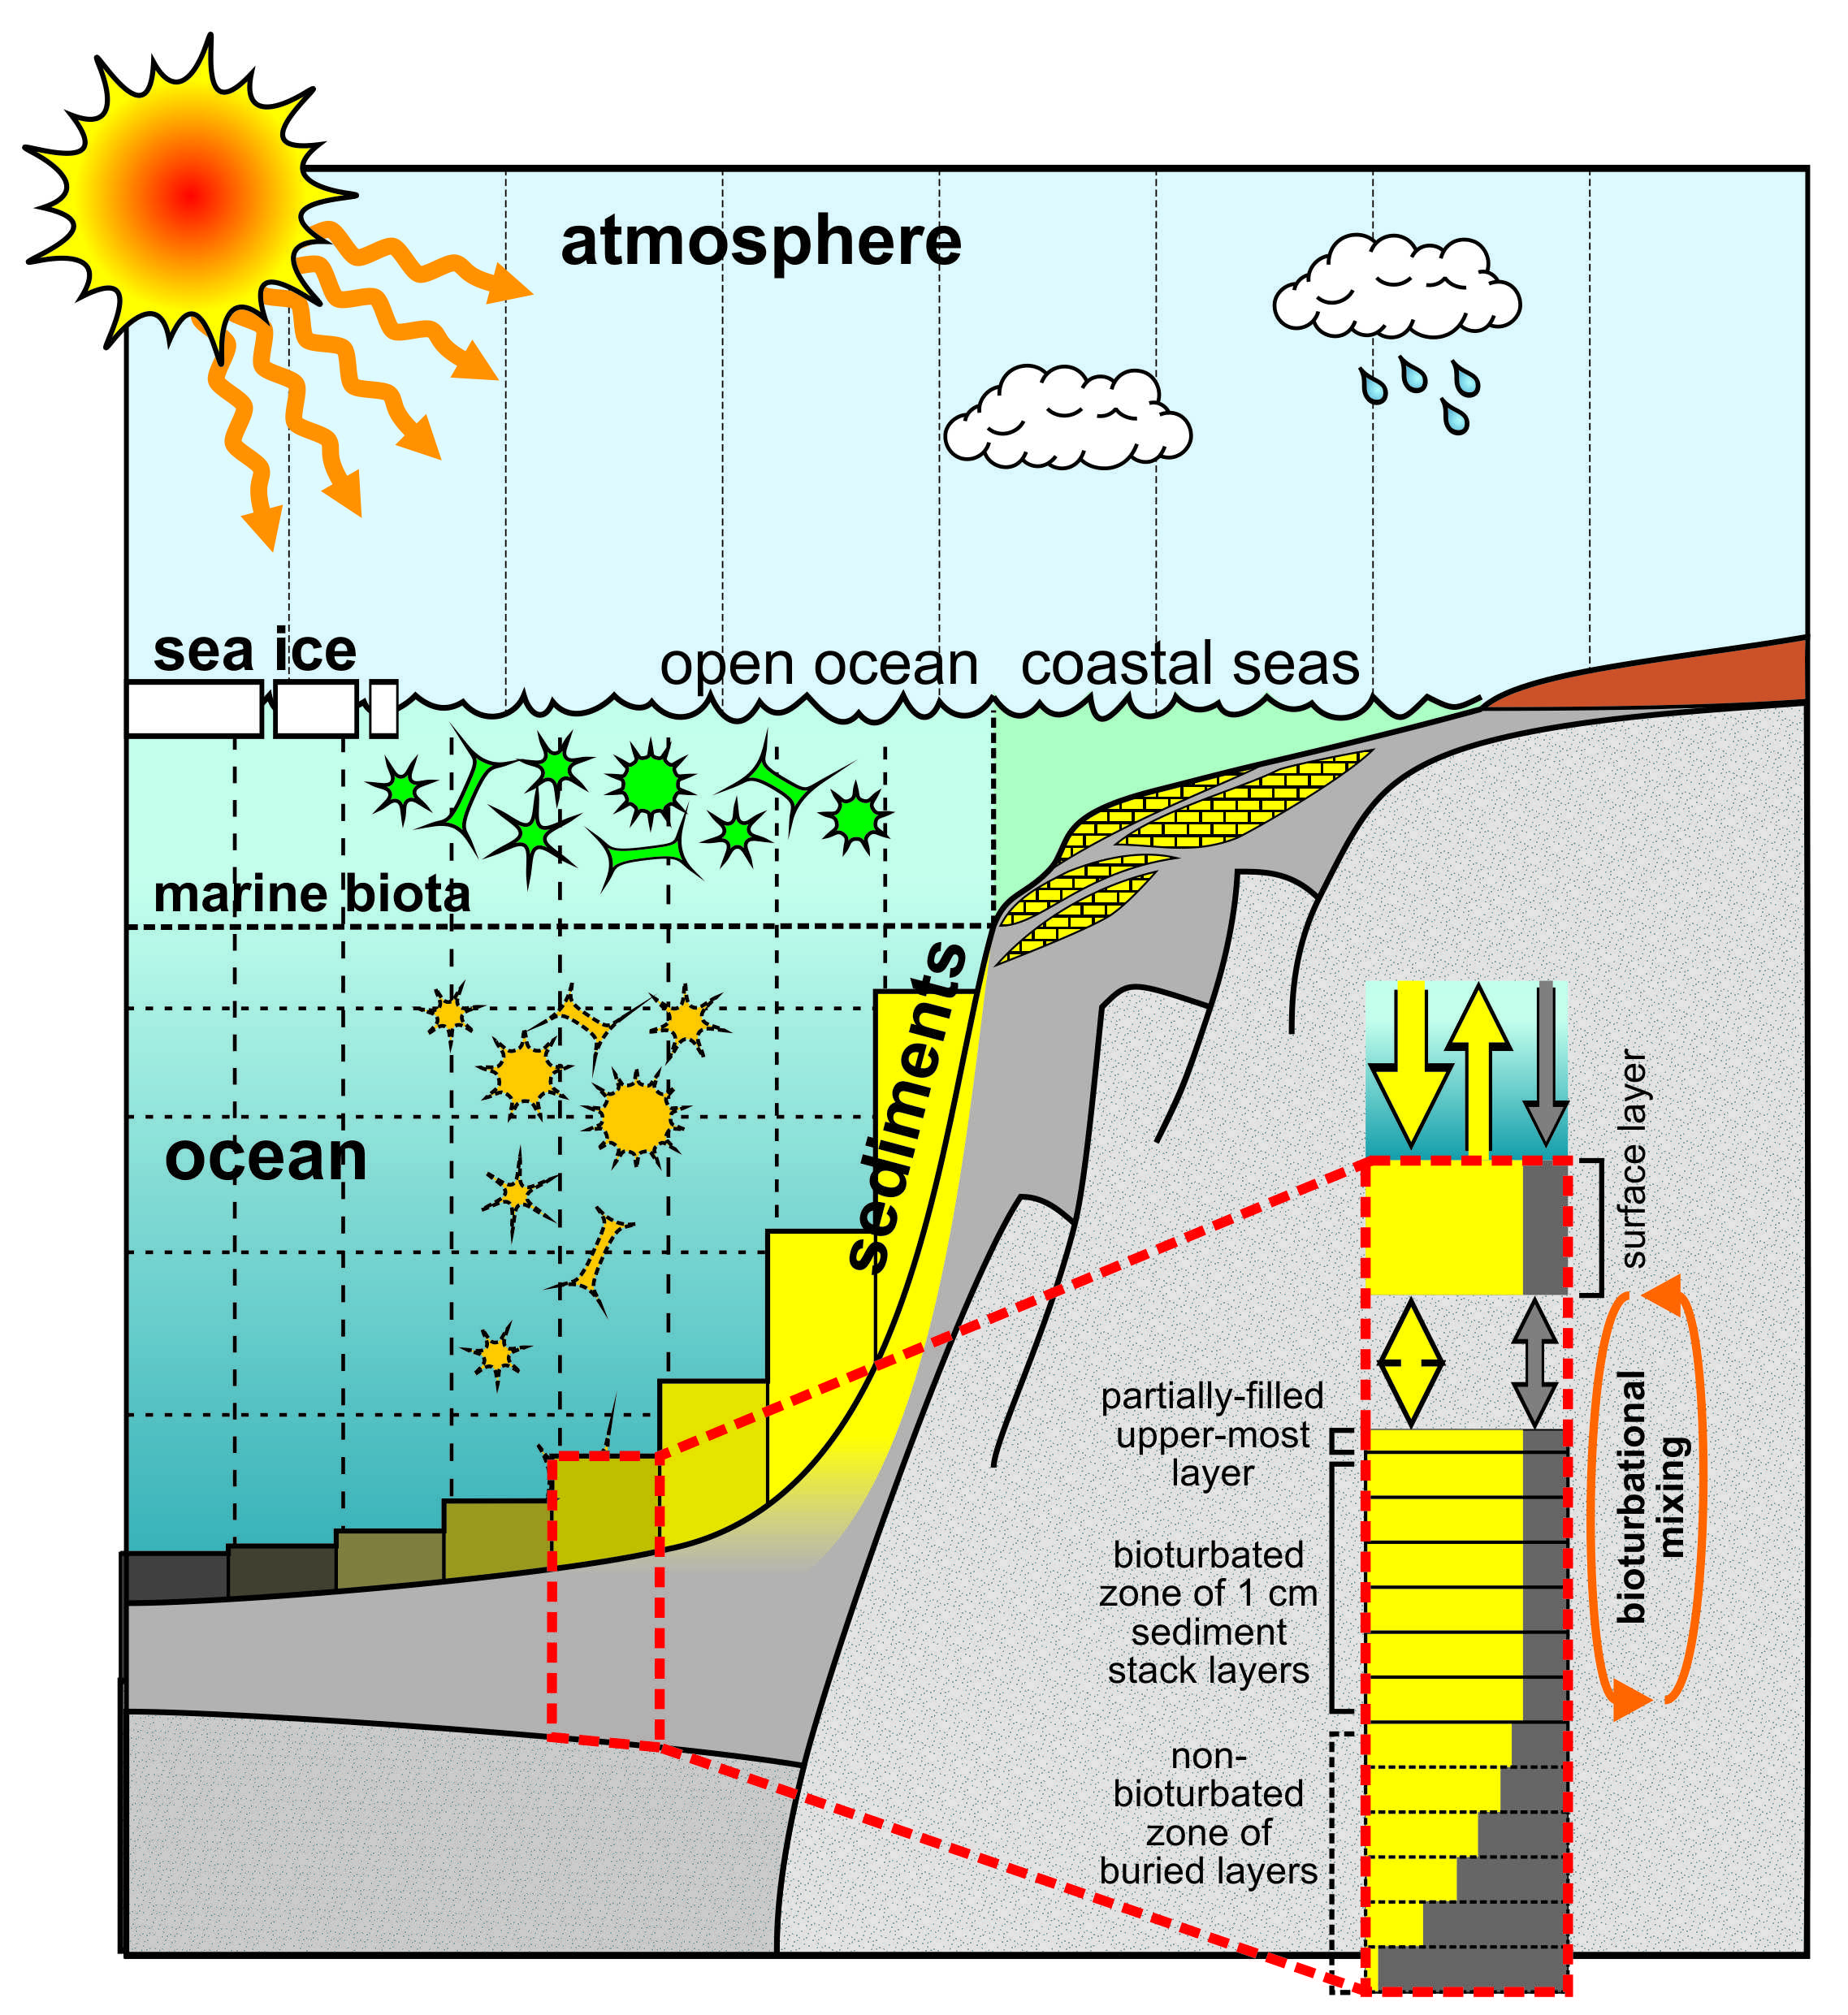
\includegraphics[width=0.5\textwidth]{sediments.jpg}
\caption{Schematic of \textbf{SEDGEM} sediment component.}
\label{fig:sediments}
\end{figure}

%------------------------------------------------
\vspace{1mm}
\noindent\rule{4cm}{0.1mm}
\vspace{2mm}
%------------------------------------------------

%------------------------------------------------
\newpage
%------------------------------------------------

\noindent Take the new model configuration for a test drive by running on from the \textit{re-start} experiment that you downloaded.

This is a steady-state climate+carbon cycle experiment that includes the deposition of \(CaCO_{3}\) in deep-sea sediments as well as the deposition of organic matter on continental shelves (plus a more minor contribution in deep-sea sediments), balanced by weathering (solute input to the ocean) plus volcanic \(CO_{2}\) out-gassing ... or at least as closely in balance as possible after 50,000 years. Try running ('briefly', but 100 years would not be too tedious for this faster configuration!) the following:

\vspace{-2mm}\small\begin{verbatim}
$ ./runmuffin.sh muffin.CBSR.fkl_pp51.BASESw
 LABS ch09.1.CTRL 100 231228.muffin.CBSR.fkl_pp51.BASESw.SPIN2
\end{verbatim}\normalsize\vspace{-2mm}

The \textit{user-config} \textsf{\footnotesize ch09.1.CTRL} is set up with the global carbon cycle configured as 'open' -- that is to say, that there is an input of carbon, alkalinity, and phosphorous to the ocean from weathering (plus carbon from volcanic out-gassing), and a loss due to preservation and burial of \(CaCO_{3}\) and organic matter in marine sediments. Depending on the state of ocean chemistry (and biology) and weathering, these two fluxes (input vs. output) do not have to balance, and hence ocean carbonate chemistry (and in turn, atmospheric \(pCO_{2}\)) can evolve with time. The \textit{spin-up} may not necessarily have the input and output fluxes absolutely perfectly balanced and hence before you run any experiments you might want to confirm whether the spin-up provided really is adequately 'spun-up'\footnote{i.e., you might plot some of the variables from the results of the \textit{spin-up}  experiment as a function of time and judge whether they are sufficiently converged or not.}. \textsf{\footnotesize ch09.1.CTRL} is hence configured to act as a control and quantify any residual flux imbalance and hence geochemical)(and climatic) 'drift'.

Note that a residual drift can be dealt with if it is relatively small and near linear via the use of a \uline{control experiment}, because any experiment you carry out will likely also incorporate (or be biased) by the same residual drift. Running a control gives you something to directly contrast  your experiment with and calculating the difference (e.g., a difference map or simple subtraction of global numbers) will give you the effect of whatever parameters you changed in the experiment but corrected for any drift. In previous exercises, you may have been a little lazy and created difference maps with respect to year 1 of an experiment -- strictly, they should have been created relative to the same year of a parallel control experiment, e.g., the results of a perturbation after 100 years should be contrasted with the year 100 results of the equivalent control.

%------------------------------------------------
\newpage
%------------------------------------------------

\noindent Before you look at any output from this experiment, you should note the following about this particular configuration and experiment:

\begin{enumerate}[noitemsep]
\vspace{1mm}
\item In the \textit{base-config} file naming convention -- the the '\textsf{\footnotesize S}' in \textsf{\footnotesize muffin.CBSR.fkl\_pp51.BASESw} specifies the use of a sediment model and the '\textsf{\footnotesize R}' a weathering module (see references should should have only just read!)\footnote{In addition to ocean and atmosphere biogeochemistry -- '\textsf{\footnotesize B}' and climate components (ocean, sea-ice, EMBM atmosphere) -- '\textsf{\footnotesize C}'.}
\vspace{1mm}
\item The '\textsf{\footnotesize w}' in \textsf{\footnotesize BASESw} specifies that a 'weathering' tracer has been included, which for simplicity, is dissolved silica. (See discussion later.)
\vspace{1mm}
\item We are running at a degraded (lower) \(18\times18\) resolution (but still \(16\) vertical levels in the ocean), and requiring fewer (twice as few in fact!) time-steps per year, for an overall approximately order-of-magnitude decrease in run-time as compared to a more standard \(36\times36\) resolution configuration of \textbf{muffin}. This is extremely helpful in being able to run \textbf{muffin} on geological time-scales but within a reasonable about of real time.
\vspace{1mm}
\item The configuration utilizes a conceptual/idealized continental configuration somewhat similar to as in the snowball Earth experiments.
\vspace{1mm}
\item Although this configuration could be regarded as a maximum complexity system, we are only going to initially look at this from the perspective of new output, and will reduce the complexity right down before we start to think about system behavior.
\vspace{1mm}
\item Data saving is set up for 2D only in \textbf{BIOGEM} (and not 3D), \textit{time-slices} only every 10000 years, and \textit{time-series} save points only every 100 years (all to minimize the size of the results files for loooooong experiment durations):
\vspace{-1mm}\small\begin{verbatim}
# force time-series saving @ 100 yr intervals
bg_par_infile_sig_name='save_timeseries_EVERY000100.dat'
# force 2D time-slice save only, and @ 10000 yr intervals
bg_ctrl_data_save_2d=.true.
bg_ctrl_data_save_3d=.false.
bg_par_infile_slice_name='save_timeslice_EVERY010000.dat'
\end{verbatim}\normalsize\vspace{-1mm}
You can return to the default saving you are used to by commenting out all these lines. Or you could change the name of the \textit{time-slice} and \textit{time-series} saving interval files, but making sure first the new file name exists (in directory: \textsf{\footnotesize genie-biogem/data/input} OR creating your own file there (and using that name).
\\Note that although a 100 year experiment will not yet have reached the first save point (with a mid-point time of 9999.5 years), \textbf{muffin} is configured to ALWAYS save you a final year \textit{time-slice}, regardless of whether your experiment duration ends up reaching a specific save point at run-end or not.
\vspace{1mm}
\item To date, the marine biochemical cycle of carbon and nutrients in muffin has included an 'implicit' alkalinity contribution (see Section 2.1 in: \textit{Ridgwell et al.} [2007]). In a fully open system with weathering and burial or organic carbon and nutrients, this becomes invalid. hence the inclusion in the \textit{user-config} of:
\vspace{-1mm}\small\begin{verbatim}
# *** BIOGEM ********************************************************
# remove organic matter associated (implicit nitrogen) alkalinity transformations
# => so we do not end up with spurious weathering ALK fluxes from kerogens 
#    (or spurious Corg burial related fluxes)
bg_par_bio_red_PON_ALK=0.0
\end{verbatim}\normalsize\vspace{-1mm}
%------------------------------------------------
\newpage
%------------------------------------------------
and in diagnosing \textbf{ROKGEM} parameter values:
\vspace{-1mm}\small\begin{verbatim}
# *** SEDGEM configuration ******************************************
# weathering diagnostic settings    
sg_par_sed_diag_P2ALK=0.0
\end{verbatim}\normalsize\vspace{-1mm}
\vspace{1mm}
\item Before we move on, a final instructive change from previously published configurations is:
\vspace{-1mm}\small\begin{verbatim}
# *** ROKGEM ********************************************************
# turn off atmospheric short circuit 
# (so CO2 is now removed from the atmosphere during weathering, 
#  and volcanic CO2 added to it)
# => to better diagnose weathering in BIOGEM output
rg_opt_short_circuit_atm=.false.
\end{verbatim}\normalsize\vspace{-1mm}
During weathering (of carbonate and silicate rocks), \(CO_{2}\) is assumed to dissolve in rainwater and reach with the calcium-bearing minerals. Later, in the ocean, when \(CaCO_{3}\) is precipitated and \(CO_{2}\) 'released'\footnote{Technically: made available for exchange with the atmosphere by a shift to lower pH.}, the \(CO_{2}\) originally removed from the atmosphere is regenerated/replaced. The 'short-circuit' is simple to assume this and not bother removing the one mol of \(CO_{2}\) in reaction with a mol of \(CaCO_{3}\) or \(CaSiO_{3}\). The \(CO_{2}\) consumption and removal from the atmosphere associated with silicate weathering is also not removed, on the basis that the alkalinity transported by rivers and added to the ocean will drive the draw-down if atmospheric \(pCO_{2}\) at that stage (rather than being removed up-front). Hence, in short-circuiting, the DIC transported to the ocean in rivers is equal to the weathering flux of carbon in \(CaCO_{3}\) plus the rate of \(CO_{2}\) out-gassing.

However, this only really 'works' if the system is in some sort of balance of weathering and precipitation and that alkalinity added to the surface ocean can fully equilibriate with the atmosphere ... which will not be the case during transient events (see Figure 3 in: \textit{Lord et al.} [2015]). Setting: \textsf{\footnotesize rg\_opt\_short\_circuit\_atm=.false.} instead tracks the \(CO_{2}\) fluxes explicitly and in full.
\\The potential implications of this will be a subject of a subsequent investigation ...
\\NOTE: A 'short-circuit' is fine if you are only looking at long-term weathering vs. sedimentation steady-states and not rapid carbon release driven transients.
\end{enumerate}

\vspace{1mm}
\noindent Other parameter settings will be introduced and explained as and when needed during this chapter.

%------------------------------------------------
\vspace{1mm}
\noindent\rule{4cm}{0.1mm}
\vspace{2mm}
%------------------------------------------------

%------------------------------------------------
\newpage
%------------------------------------------------

\section{Sediment model output}

There is a whole new set of additional outputs from this configuration of \textbf{muffin}, particularly sediment-specific output from the \textbf{SEDGEM} module and which is saved in the \textsf{\footnotesize sedgem} sub-directory of the main experiments results directory. Data saving differs from \textbf{BIOGEM} in that the composition of the sediments (and other diagnostics such as rain and dissolution fluxes) is saved only \uline{at the very end} of a model experiment (hence unlike \textbf{BIOGEM}, which by default saves a series of time-slices throughout the course of a model experiment). So if you kill a run before the very end (or the run crashes),  \uline{you will get no} (or little) \textbf{SEDGEM} output.

2D (e.g. surface sediment properties, fluxes, etc.) results can be found in  the \textsf{\footnotesize sedgem} sub-directory of your experiment directory  in a \textbf{netCDF} file called \textsf{\footnotesize fields\_sedgem\_2d.nc}. For example, the 2D distribution of \(wt\% CaCO_{3}\) –- which is the weight fraction of calcium carbonate (\(CaCO_{3}\)) in the surface sediments of the deep ocean (i.e., how much plankton carbonate shell material is there compared to other stuff in the mud at the bottom of the ocean), is saved in this \textbf{netCDF} file under a variable called: \textsf{\footnotesize sed\_CaCO3}. Note that there is some duplication of results saving, because a series of \textit{time-slices} of sediment composition are also saved in the 2D \textbf{BIOGEM} netCDF file \textsf{\footnotesize fields\_biogem\_2d.nc}. \textbf{BIOGEM} also saves a selection of \textit{time-series }of sediment properties -- \textsf{\footnotesize .res} files starting \textsf{\footnotesize biogem\_series\_sed}. For example, the \textit{time-series} file: \textsf{\footnotesize biogem\_series\_sed\_CaCO3.res} contains information about how the mean \(CaCO_{3}\) content of surface sediments (uppermost sediment layer) evolves with time. There are also \textit{time-series} file output that record the evolution of burial (and dissolution) fluxes as well as weathering -- all of which will be important for fully understanding system behavior.

As per with \textbf{BIOGEM} data saving, \textbf{SEDGEM} also saves a summary file of sediment fluxes and composition -- \textsf{\footnotesize seddiag\_misc\_DATA\_GLOBAL.res} as well as a parameter valiue summary for use in configuring \textbf{ROKGEM} (discussed later) -- \textsf{\footnotesize seddiag\_misc\_ROKGEM\_parameters.res}

%------------------------------------------------
\vspace{1mm}
\noindent\rule{4cm}{0.1mm}
\vspace{2mm}
%------------------------------------------------

\noindent The model also generates artificial sediment ‘cores’ (e.g. see: \textit{Ridgwell} [2007]) and hence what one might expect to see of your applied perturbations as recorded in a sediment core sand then recovered from the ocean floor(!) In the \textbf{SEDGEM} results sub-directory, there is a \textbf{netCDF} file which contains all the locations selected (if any) –- \textsf{\footnotesize sedcore.nc}. These are not really aligned with latitude as the \textbf{Panoply} display might suggest – the locations are in fact distributed from all over the ocean (\textbf{Panoply} is being fooled in order to display them together). In the \textbf{SEDGEM} 2D \textbf{netCDF} file, these locations are marked in the \textbf{netCDF} variable \textsf{\footnotesize grid\_mask\_sedcore}. The locations of these cores are stored in a a file containing a little ASCII ‘map’ of the ocean.
\vspace{1mm}

\begin{itemize}[noitemsep]
\vspace{1mm}
\item
If you are using a 'paleo' configuration of \textbf{muffin}, indicated by a parameter section in the \textit{base-config} file headed by something looking like:
\footnotesize\begin{verbatim}
# *******************************************************************
# GRID & BOUNDARY CONDITION CONFIGURATION
# *******************************************************************
# insert the automatically generated muffingen parameter list here
# *******************************************************************
##################################################################################
### cGENIE .config file parameter lines generated by muffingen v0.9.21 on: 220314 ###
\end{verbatim}\normalsize
then there will be a parameter line that direct muffin to look for \textbf{SEDGEM} configuration files in the respective \textsf{\footnotesize genie-paleo } directory, e.g.:
\vspace{-1mm}\small\begin{verbatim}
sg_par_pindir_name='../../cgenie.muffin/genie-paleo/fkl_pp51/'
\end{verbatim}\normalsize\vspace{-1mm}
\vspace{1mm}
\item Otherwise, the file lives in: \textsf{\footnotesize cgenie.muffin/genie-sedgem/data/input}
\end{itemize}
\vspace{1mm}
The filename is given by the parameter: \texttt{sg\_par\_sedcore\_save\_mask\_name}
\\Simply be editing (using the ASCII text editor) a '0.0' to a '1.0', you can get the model to generate and save a sediment ‘core’ at that particular (\textit{i,j}) location.

%------------------------------------------------
\vspace{1mm}
\noindent\rule{4cm}{0.1mm}
\vspace{2mm}
%------------------------------------------------

\noindent \textbf{netCDF} file \textsf{\footnotesize sedcore.nc } variables include:

\vspace{1mm}
\begin{itemize}[noitemsep]
\item \textsf{\footnotesize phys\_layer } –- sediment layer number (counting down).
\item \textsf{\footnotesize phys\_depth } -– (cumulative) depth below surface, measured from the sediment surface to the mid-point of each sediment layer (cm).
\item \textsf{\footnotesize th (cm) } -- thickness of each sediment layer (cm).
\item \textsf{\footnotesize age\_CaCO3 } -- the mean age of \(CaCO_{3}\) particles in a sediment layer.
\\Note that this will not be defined if there is no \(CaCO_{3}\) preserved.
\item \textsf{\footnotesize ... } then some alternative ways of assigning a chronology to a sediment core … (ignore) ...
\item \textsf{\footnotesize phys\_porosity  } -- sediment layer density (as if you cared!).
\item \textsf{\footnotesize sed\_POC } and \textsf{\footnotesize sed\_POC\_13C } -- mean organic matter content of each sediment layer and its \(\delta^{13} C\). But note: in this configuration no organic matter is preserved (hence all zeros for POC).
\item \textsf{\footnotesize sed\_CaCO3} and \textsf{\footnotesize sed\_CaCO3\_13C } -- mean \(CaCO_{3}\) content (wt\%) of each sediment layer and its \(\delta^{13} C\).
\item \textsf{\footnotesize sed\_det } and \textsf{\footnotesize sed\_ash } -- the wt\% detrital and ‘ash’ contents of a layer (ash is used as a conservative numerical sediment tracer in order to mark the depth of the start of the experiment).
\end{itemize}
\vspace{1mm}

\noindent Obviously – you could plot e.g. \(CaCO_{3}\) (or its \(\delta^{13}C\)) as a function of depth and/or age across and see how your carbon release experiment might be recorded in the marine geological record (e.g., how does this compare with observations across events such as the PETM?).

Note that the sediment cores reflect not only the material which has accumulated (or not, if it has dissolved …) during the course of your experiment, but also the material that accumulated during the spin-up. PLUS, whatever material the sediment core was initialized with to start with. For example, the large interval of initially 100\% detrital material at the base of the sediment core simply reflects the initialization of the sediment array in the model. Also note the ash ‘peak’ near the bottom of the stack (filled) sediment layers – this is a tracer to ‘tag’ the start of the model spin-up. If you look at the spin-up results (not your recent perturbation experiment) – the ash peak lies in a sediment layer with age equal to the total length of of the spin-up carried out. But why is there any ash deeper than the age corresponding to the start of the spin-up? How can it get there (i.e. what processes could move solid material deeper within the sediment column)?

%------------------------------------------------
\vspace{1mm}
\noindent\rule{4cm}{0.1mm}
\vspace{2mm}
%------------------------------------------------

\noindent If the provided experiment configuration does not specify the creation of any sediment cores -- go ahead and define some by editing file \textsf{\footnotesize fkl\_pp51.sedcoremask.dat} in: \textsf{\footnotesize cgenie.muffin/genie-paleo/fkl\_pp51} and flipping a '0.0' to a '1.0'. Then run a new experiment (copy-paste the \textit{user-config} and rename) for e.g., 100 years again as above and look for the additional (sediment core) output.

%------------------------------------------------
\newpage
%------------------------------------------------

Published examples of simulated marine sediment core output include (in order of publication date):
\begin{itemize}[noitemsep]
\item Ridgwell, A., Interpreting transient carbonate compensation depth changes by marine sediment core modeling, Paleoceanography 22, PA4102, doi:10.1029/2006PA001372 (2007).
\item Kirtland Turner, S., and A. Ridgwell, Recovering the true size of an Eocene hyperthermal from the marine sedimentary record, Paleoceanography (2013).
\item Jennions, S M., E. Thomas, D.N. Schmidt, D. Lunt, and A. Ridgwell, Changes in benthic ecosystems and ocean circulation in the Southeast Atlantic across Eocene Thermal Maximum 2, Paleoceanography DOI: 10.1002/2015PA002821 (2015).
\item Penman, D.E., S.Kirtland Turner, P. Sexton, R. Norris, A.J. Dickson, S. Boulila, A. Ridgwell, R.E. Zeebe, J. Zachos, A. Cameron, T. Westerhold, U. Röhl, IODP Expedition 342 Scientists, An abyssal carbonate compensation depth overshoot in the aftermath of the Palaeocene- Eocene Thermal Maximum, Nature Geoscience 9, doi:10.1038/NGEO2757 (2016).
\item (in the SI) Gutjahr, M., A. Ridgwell, P.F Sexton, E. Anagnostou, P.N. Pearson, H. Pälike, R.D. Norris, E. Thomas, and G.L. Foster, Very large release of mostly volcanic carbon during the Paleocene-Eocene Thermal Maximum Paleocene-Eocene Thermal Maximum, Nature 548, doi:10.1038/nature23646 (2017).
\item Fantle, M. S., and A. Ridgwell, Towards an understanding of the Ca isotopic signal related to ocean acidification and alkalinity overshoots in the rock record, Chemical Geology DOI: 10.1016/j.chemgeo.2020.119672 (2020).
\end{itemize}
and you might want to think about how you might make use of the \textit{sedcore} output in light of these papers.

%------------------------------------------------
\newpage
%------------------------------------------------

\section{Quantifying how long is the 'long tail' of CO$_{2}$}

The 'full' geological carbon cycle is complex ... we'll pick it apart soon ... but you may as well have a quick 'play'. Regardless, highly idealized perturbations are the way to go first. Specifically -- an illustrative experiment which has a parallel to experiments you have conducted previously, is to add a pulse \(CO_{2}\) release to the atmosphere and track the consequences for atmospheric p\(CO_{2}\) and ocean chemistry (particularly ‘alkalinity’), and now also e.g. deep sea sediments. 

\vspace{1mm}
In the \textsf{\footnotesize ch09.3.EXPT} \textit{user-config}, the lines:
\vspace{-2mm}\small\begin{verbatim}
bg_par_forcing_name='pyyyyz.FpCO2_Fp13CO2'
bg_par_atm_force_scale_val_3=8.3333e+016
bg_par_atm_force_scale_val_4=-15.0
\end{verbatim}\normalsize\vspace{-2mm}
specify the release of \(CO_{2}\) to the atmosphere at a rate of \(0.1 PgC yr^{-1}\) with an isotopic composition of \(-15\)\permille -- appropriate for a volcanic-related geological source. The lines:
\vspace{-2mm}\small\begin{verbatim}
bg_par_atm_force_scale_time_3=10000.0
bg_par_atm_force_scale_time_4=10000.0
\end{verbatim}\normalsize\vspace{-2mm}
then specify that this input (and isotopic composition) continues over 10,000 years.

\vspace{1mm}
Unless you wish to run an experiment for 10,000 years or more (yawn!!), you might want to reduce the interval emissions are over (changing both parameter values equally) as well as increasing the emissions rate (as you did in earlier exercises). You could also consider isotopic compositions of \(-27\)\permille -- appropriate for a fossil fuel carbon source, or methane derived carbon (e.g., as from hydrates) which would be more like \(-60\)\permille and create a more exciting carbon isotopic perturbation to watch. For example, perhaps something like:
\vspace{-2mm}\small\begin{verbatim}
# specify forcings -- 5,000 PgC @ -60 o/oo over 100 yr
bg_par_forcing_name="pyyyyz.FpCO2_Fp13CO2"
bg_par_atm_force_scale_val_3=8.3333e+013
bg_par_atm_force_scale_val_4=-60.0
bg_par_atm_force_scale_time_3=100.0
bg_par_atm_force_scale_time_4=100.0
\end{verbatim}\normalsize\vspace{-2mm}
would be like a slightly super-charged anthropogenic experiment\footnote{50 PgC per year for 100 years, as opposed to the current ca. 10 PgC per year.} and with more a more pronounced isotopic fingerprint. Or configure the same emissions as you might have explored before\footnote{(e.g., 1000 PgC over 1 year)} .

\vspace{1mm}
Run the model for as long as you dare (or can be bothered) – 1,000 or 2,000 years might be just enough  to start to see impacts on deep-sea sediments, but 10,000 years or more would be much better. (You can always submit this to the cluster queue and get on with something else.) FYI: 10,000 years is going to take something like an hour ... if you are lucky ...

Remember the earlier comment earlier in the chapter about the frequency of output saving -- you may well want at the very least, more frequent \textit{time-series} saving\footnote{Comment out to obtain default saving intervals, or change a save interval definition file with a shorter regular spacing in time.}.

Plot the time-series of e.g. atmospheric \(pCO_{2}\) and compare to the (much shorter experiments) you have carried out before with a simple ocean+atmosphere only system. Compare how quickly atmospheric \(pCO_{2}\) decays compared to previously \textbf{muffin} publications (e.g., \textit{Ridgwell and Hargreaves} [2007]) or other models (e.g. \textit{Archer et al.} [2009]) and  how the sediments respond (e.g. the time-series of sediment \(CaCO_{3}\) content).

%------------------------------------------------
\newpage
%------------------------------------------------

\noindent BE CAREFUL -- if you have previously edited the \textit{forcing} \textsf{\footnotesize  pyyyyz.FpCO2\_Fp13CO2}, you are going to need to return whatever files you edited back to their original state.
\small\begin{enumerate}[noitemsep]
\vspace{1mm}
\item From \textsf{\footnotesize genie-main}, \texttt{\$ make cleanall}
\vspace{1mm}
\item Then head up a directory level (\texttt{cd ..}) to \textsf{\footnotesize cgenie.muffin}
\vspace{1mm}
\item Type: \texttt{\$ git status -uno}
\vspace{1mm}
\\You should see a list of all files originally cloned from GitHub) that have changed, e.g.:
\vspace{-1mm}\begin{verbatim}
modified:   genie-forcings/pyyyyz.FpCO2_Fp13CO2/biogem_force_flux_atm_pCO2_sig.dat
\end{verbatim}\vspace{-1mm}
(Note that files you create are not listed. TO see those, type: \texttt{\$ git status})
\vspace{1mm}
\item To restore the state of any file that you might have edited, \texttt{git checkout} that file out, e.g.:
\vspace{-1mm}\begin{verbatim}
$ git checkout genie-forcings/pyyyyz.FpCO2_Fp13CO2/biogem_force_flux_atm_pCO2_sig.dat
\end{verbatim}\vspace{-1mm}
\end{enumerate}\normalsize

%------------------------------------------------
\vspace{1mm}
\noindent\rule{4cm}{0.1mm}
\vspace{2mm}
%------------------------------------------------

\noindent DON'T FORGET -- Did you remember to run a control experiment? The same experiment\footnote{(Just copy-paste and then rename \textsf{\footnotesize ch09.3.EXPT} -> \textsf{\footnotesize ch09.3.CTRL} or similar.}  you have probably just pressed \textsf{\footnotesize return} on, but with the rate of carbon emissions set to zero (no other changes ... run for the same experiment duration ...).

%------------------------------------------------
\vspace{1mm}
\noindent\rule{4cm}{0.1mm}
\vspace{2mm}
%------------------------------------------------

\noindent To properly (quantitatively) appreciate the role of ocean-sediment interaction (and weathering) and controlling atmospheric \(pCO_{2}\), you need to contrast these experiments with as similar a model configuration as possible -- for instance, one that is identical excepting having no sediments (or weathering). 

You can achieve this quite simply: create (/copy-rename) a new \textit{user-config} based on \textsf{\footnotesize ch09.3.EXPT} and edit the lines\footnote{You do not have to edit the comment line (\#) but it will help you remember what you have done.}:
\vspace{-1mm}\small\begin{verbatim}
# set an 'OPEN' system
bg_ctrl_force_sed_closedsystem=.false.
\end{verbatim}\normalsize\vspace{-1mm}
changing it to:
\vspace{-1mm}\small\begin{verbatim}
# set a 'CLOSED' system
bg_ctrl_force_sed_closedsystem=.true.
# automatically seed all weathering fluxes as non-zero
rg_ctrl_force_sed_closedsystem=.TRUE.
\end{verbatim}\normalsize\vspace{-1mm}

\noindent What this  does is to force the model to always maintain an exact balance between the preservation and burial in marine sediments of \(CaCO_{3}\) and organic matter (both carbon and nutrients), with the supply of solutes derived from the weathering of \(CaCO_{3}\), \(CaSiO_{3}\), organic matter, and apatite (for phosphate) on land, plus volcanic out-gassing. Because no excess or deficit of weathering vs. sedimentation is allowed to occur, no changes in ocean chemistry (other than by air-sea gas exchange) occur. This configuration hence acts (geochemically and dynamically) exactly the same way as a configuration without any sediments or weathering being present (and as used previously). 

However, for this setting to work properly, you do need to flip 'short-circuiting' back on to ensure that \(CO_{2}\) is not being removed and hence being drained from the atmosphere, and hence set: \texttt{rg\_opt\_short\_circuit\_atm=.false.}

%------------------------------------------------
\newpage
%------------------------------------------------

By comparing the two experiments (with and without a 'closed system', and also both with the control): can you deduce the effect of the sediment and weathering interactions and feedbacks in modulating (accelerating or decelerating) atmospheric \(pCO_{2}\) decline?\footnote{e.g. you could compare the \(pCO_{2}\) time-series of the 2 different experiments, or create anomalies from both with respect to the control, and then contrast.}

Also view the sediment distribution (of \(CaCO_{3}\)): what are the impacts on sediment composition in the case of an experiment configured with an ‘open’ system (vs. a 'closed' system)? Here, the time-series file of mean global sediment composition \textsf{\footnotesize biogem\_series\_sed\_CaCO3.res} (in units of: \(wt\%\:CaCO_{3}\)) may help illustrate what is going on here.
Note that the way the ‘closed’ system is constructed; a response of the sediments is predicted and saved in the output, even though it is not allowed to affect chemistry or atmospheric p\(CO_{2}\).

%------------------------------------------------
\vspace{1mm}
\noindent\rule{4cm}{0.1mm}
\vspace{2mm}
%------------------------------------------------

\noindent To recap -- you are aiming to run a \(CO_{2}\) emissions experiment using a \textbf{muffin} configuration including variable weathering and sedimentation (\textsf{\footnotesize ch09.3.EXPT}) with a version/copy that you have edited to create a 'closed' ocean-atmosphere system, with no ocean-sediment or weathering feedbacks on atmospheric \(CO_{2}\). Ideally, you would also run a PAIR (not just one!) of control experiments -- one for each of 'open' and 'closed' configurations and each with no \(CO_{2}\) emissions specified. (A total of 4 experiments.)

%------------------------------------------------
\newpage
%------------------------------------------------

\section{Sediments of the modern Earth}

Having had a quick 'play' with the system, we should return -- albeit briefly -- to reality and critically and quantitatively assess to what degree \textbf{muffin}  provides an adequate representation of the interaction between ocean chemistry and sediment composition (e.g., in \(CaCO_{3}\) buffering of \(CO_{2}\) release and 'carbonate compensation'). Key to this, is contrasting  model output against observational-based data. Such an approach is presented in \textit{Ridgwell and Hargreaves} [2007]. Note that the following experiments, for which you are NOT provided \textit{restarts} for, take a few days to run and you might consider getting these\footnote{Although the 2nd-stage \textit{spin-up} will require the first stage one to complete.} on the cluster queue and work on the next section (or more experiments from the previous one) while they run.

\vspace{1mm}
The required \textit{base-} and \textit{user-config} files are both provided as part of the \textbf{muffin} code release:

\begin{itemize}[noitemsep]
\vspace{1mm}
\item \textsf{\footnotesize muffin.CBSR.p\_worbe2.BASES} -- the \textit{base-config} file, including \textbf{SEDGEM} (the '\textsf{\footnotesize S}' in '\textsf{\footnotesize CBSR}' and \textbf{ROKGEM} -- '\textsf{\footnotesize R}') modules.
\vspace{1mm}
\item \textsf{\footnotesize muffin.CBSR.p\_worbe2.BASES.RidgwellHargreaves1997\_S36x36.SPIN1} -- the \textit{user-config} for the 1st stage (20 kyr long) \textit{spin-up} described in \textit{Ridgwell and Hargreaves} [2007]. This file lives in the \textsf{\footnotesize EXAMPLES} sub-directory of \textsf{\footnotesize genie-userconfigs}.
\end{itemize}

This can then be run:
\vspace{-1mm}\small\begin{verbatim}
./runmuffin.sh muffin.CBSR.p\_worbe2.BASES EXAMPLES
   muffin.CBSR.p_worbe2.BASES.RidgwellHargreaves1997_S36x36.SPIN1 20000
\end{verbatim}\normalsize\vspace{-1mm}

Read the paper and consider the plotted core-top sediment composition data-set (and ideally, \uline{read the associated cited papers by David Archer}). Does the model get the broad patterns right (is it more right than wrong, or more wrong than right)? Do you think the model-data misfits might be important? How so?

%------------------------------------------------
\vspace{1mm}
\noindent\rule{4cm}{0.1mm}
\vspace{2mm}
%------------------------------------------------

\noindent A \textit{user-config} for the second-stage spin-up as described in \textit{Ridgwell and Hargreaves} [2007] is also provided:
\begin{itemize}[noitemsep]
\vspace{1mm}
\item \textsf{\footnotesize muffin.CBSR.p\_worbe2.BASES.RidgwellHargreaves1997\_S36x36.SPIN2} is the 2nd-stage, 50 kyr \textit{spin-up} that uses \textsf{\footnotesize muffin.CBSR.p\_worbe2.BASES.RidgwellHargreaves1997\_S36x36.SPIN1} as a \textit{re-start}.
\end{itemize}
\vspace{1mm}
and can be run:
\vspace{-1mm}\small\begin{verbatim}
./runmuffin.sh muffin.CBSR.p\_worbe2.BASES EXAMPLES
   muffin.CBSR.p_worbe2.BASES.RidgwellHargreaves1997_S36x36.SPIN2 50000
   muffin.CBSR.p_worbe2.BASES.RidgwellHargreaves1997_S36x36.SPIN1
\end{verbatim}\normalsize\vspace{-1mm}

Having run the second spin-up, which now includes a full bioturbated sediment depth of \(CaCO_{3}\) that can potentially be reacted with \(CO_{2}\) added to the system (see: \textit{Ridgwell and Hargreaves} [2007] and also \textit{Ridgwell} [2007]), you could try and perturbation experiment. All you need to do, is take \textsf{\footnotesize muffin.CBSR.p\_worbe2.BASES.RidgwellHargreaves1997\_S36x36.SPIN2}, copy-and-rename as per usual, and then change the \textit{forcing}.

%------------------------------------------------
\newpage
%------------------------------------------------

The current \textit{forcing} is:
\vspace{-1mm}\small\begin{verbatim}
# specify forcings -- ONLY apply a non-carbonate (detrital) flux (to the sediments)
bg_par_forcing_name="worbe2.detplusopalSED"
\end{verbatim}\normalsize\vspace{-1mm}
This specifies a 'detrital' field -- basically the rate of accumulation of non carbonate solids in the sediments (see: \textit{Ridgwell and Hargreaves} [2007] and references there-in). You need to retain this specified detrital flux forcing, but add a \(CO_{2}\) one to the atmosphere. One is provided in the \textit{forcings} directory\footnote{\textsf{\footnotesize worbe2.FpCO2\_Fp13CO2.detplusopalSED}}, but more instructive is to adapt the current one. To do this:
\begin{enumerate}[noitemsep]
\vspace{1mm}
\item Copy-and-rename the forcing folder that is currently pointed to -- \textsf{\footnotesize worbe2.detplusopalSED}.
\vspace{1mm}
\item Find a previous experiment where you released \(CO_{2}\) to the atmosphere, and find the \textit{forcing} folder used for that\footnote{It may well have been called something like: \textsf{\footnotesize pyyyyz.FpCO2\_Fp13CO2}}.
\vspace{1mm}
\item Three files in the \(CO_{2}\) emissions \textit{forcing} folder together define a \(CO_{2}\) flux is to be used:
\\\textsf{\footnotesize configure\_forcings\_atm.dat}
\\\textsf{\footnotesize biogem\_force\_flux\_atm\_pCO2\_sig.dat}
\\\textsf{\footnotesize biogem\_force\_flux\_atm\_pCO2\_13C\_sig.dat}
\\(If you have forgotten what these are/do -- refer back to the ocean circulation and/or fossil fuel emissions chapters.)
\\Simply copy these 3 files into your new \textit{forcing} folder.
\vspace{1mm}
\item Change the name of the forcing in your \textit{user-config}, and scale the \(CO_{2}\) flux as per you did earlier, e.g., adding:
\vspace{-1mm}\small\begin{verbatim}
bg_par_atm_force_scale_val_3=8.3333e+013
bg_par_atm_force_scale_val_4=-27.0
\end{verbatim}\normalsize\vspace{-1mm}
This would give you just \(1 PgC yr^{-1}\) (at \(-27\)\permille), so you need to adjust this (refer to earlier in this chapter, and to earlier chapters).
\end{enumerate}

%------------------------------------------------
\vspace{1mm}
\noindent\rule{4cm}{0.1mm}
\vspace{2mm}
%------------------------------------------------

\noindent How the 2nd stage spin-up is derived from the results of the first and how either \textit{user-config} is constructed in the first place, we will look at in the next section. For now, just note the following about the two provided experiment configurations:

\vspace{1mm}

\begin{itemize}[noitemsep]
\vspace{1mm}
\item SPIN1 is 'closed':
\vspace{-1mm}\small\begin{verbatim}
rg_ctrl_force_sed_closedsystem=.TRUE.
\end{verbatim}\normalsize\vspace{-1mm}
\vspace{1mm}
\item SPIN1 sets a parameter value that is not used in the experiment itself, but informs the calculation of the \textbf{ROKGEM} parameters for use in SPIN2:
\vspace{-1mm}\small\begin{verbatim}
sg_par_sed_diag_fracSiweath=0.0
\end{verbatim}\normalsize\vspace{-1mm}
\vspace{1mm}
\item SPIN2 has a section of parameters that were automatically-generated -- the section starting:
\vspace{-1mm}\small\begin{verbatim}
 # --- ROKGEM USER-CONFIG --------
 # NOTE: automatically generated by SEDGEM
\end{verbatim}\normalsize\vspace{-1mm}
\end{itemize}

%------------------------------------------------
\newpage
%------------------------------------------------

\section{The marine geology of fake worlds}

You can configure any of your previous fake worlds, or generate new ones, to have a full geologic carbon cycle including deposition of \(CaCO_{3}\) in marine sediments and weathering on land.

In order to generate the requisite \textbf{SEDGEM} configuration files, you need the following settings in your \textbf{muffingen} configuration file:

\begin{itemize}[noitemsep]
\vspace{1mm}
\item \texttt{opt\_makeseds=true;} --  requests that \textbf{SEDGEM} files are generated.
\vspace{1mm}
\item \texttt{par\_sedsopt=2;} -- requests that a randomized bathymetry is generated. This is needed because fake worlds have by default, a flat bathymetry.
\\Instead, if you 'draw' a non-uniform bathymetry, you would set:
\\ \texttt{par\_sedsopt=0;} -- requests that the ocean depth levels ('k1' file') are used to inform the ocean floor depth assumed by \textbf{SEDGEM}.
\\(Option \texttt{1} is most commonly used in conjunction with a GCM-derived continental configuration.)
\end{itemize}

\vspace{1mm}
So, if you define continents in your fake world, but do not change the bathymetry in \textbf{muffingen}, \texttt{par\_sedsopt} option \texttt{2} will give you a randomized distribution of sediment depths (used in the \(CaCO_{3}\) solubility pressure calculation only). Selecting option \texttt{0} will simply translate your chosen \textbf{muffingen} ocean depths into \textbf{SEDGEM} depths. Note that you can still have a flat bottom to the ocean (no variation in ocean floor depth) and choose option \texttt{0}.

If you define a specific bathymetry by hand (e.g. draw in ocean ridges), you probably do not want it over-written (by a random \textbf{SEDGEM} depth pattern) and hence you should chose option \texttt{0}.

For speed of running model experiments, it is recommended that you generate your \textbf{muffingen} \textbf{muffin} configurations at the lowest reasonable resolution -- \(18\times18\times8\) would be suitable -- \(18\times18\) resolution in lon vs. lat, and \(8\) levels in the ocean. (You could try pushing this a little further and more extreme, e.g. \(12\times12\times8\).) Note that when you create your \textit{base-config}, you should use the template:
\vspace{1mm}
\\\textsf{\footnotesize CONFIG\_template\_08lvl\_R07.config}
\vspace{1mm}
\\(for the 8-level ocean, rather than \textsf{\footnotesize CONFIG\_template\_16lvl\_R07.config } which is designed for 16-ocean level configurations).

Once you have copy-pasted the configuration output of \textbf{muffingen} into the template \textit{base-config} file (and suitably renamed it), you need to enable the geologic carbon cycle modules (\textbf{SEDGEM} and \textbf{ROCKGEM}). At the top of the \textit{base-config} file, ensure that the following are set:
\vspace{-1mm}\small\begin{verbatim}
ma_flag_sedgem=.TRUE.
ma_flag_rokgem=.TRUE.
\end{verbatim}\normalsize\vspace{-1mm}
And then, further down and under the heading:
\vspace{-1mm}\small\begin{verbatim}
# TRACER CONFIGURATION
\end{verbatim}\normalsize\vspace{-1mm}
you need to define how many 'tracers' in the ocean, what they are, and any initial values that differ from modern defaults. Plus, whatever atmospheric and sediment tracers you want (plus default values in the atmosphere). Simplest at this point is to copy-paste from an existing \textit{base-config}, such as:
\vspace{1mm}
\\\textsf{\footnotesize cgenie.eb\_go\_gs\_ac\_bg\_sg\_rg.worbe2.BASE}
\vspace{1mm}
\\(which is the \textit{base-config} used in \textit{Ridgwell and Hargreaves} [2007]).

\vspace{1mm}
As for a suitable \textit{user-config} ...

... you could take the \textit{user-config} from \textit{Colbourn et al.} [2013] (itself a modification of Ridgwell and Hargreaves [2007]) -- available as part of the \textbf{muffin} code release, as file:
\vspace{1mm}
\\\textsf{\footnotesize EXAMPLE.worbe2.Colbournetal2013.CTRL } (\textsf{\footnotesize genie-userconfigs } sub-directory)
\vspace{1mm}
\\Then generalize this according to the paleo sediment configuration used in \textit{Ridgwell and Schmidt} [2010] (file: \textsf{\footnotesize EXAMPLE.p0055c.RidgwellSchmidt2010.SPIN1 } in the \textsf{\footnotesize genie-userconfigs } sub-directory) (i.e. making \(CaCO_{3}/POC\) export invariant, adding a fixed detrital flux to the sediments).

Cutting the lines down to the bare minimum (excepting comments pertaining to new/altered lines), a suitable \textit{user-config} then looks like:

\scriptsize\begin{verbatim}
# --- CLIMATE --------------------------------------------------
# enable CO2 climate feedback
ea_36=y
# --- BIOLOGICAL NEW PRODUCTION --------------------------------
bg_par_bio_k0_PO4=1.9582242E-06
bg_par_bio_c0_PO4=2.1989611E-07
# --- ORGANIC MATTER EXPORT RATIOS -----------------------------
bg_par_bio_red_DOMfrac=0.66
# --- INORGANIC MATTER EXPORT RATIOS ---------------------------
# set fixed export CaCO3 as a proportion of particulate organic matter
bg_par_bio_red_POC_CaCO3=0.200
bg_par_bio_red_POC_CaCO3_pP=0.0
# --- REMINERALIZATION -----------------------------------------
bg_par_bio_remin_DOMlifetime=0.5
bg_par_bio_remin_POC_frac2=6.4591110E-02
bg_par_bio_remin_POC_eL1=550.5195
bg_par_bio_remin_POC_eL2=1000000.0
bg_par_bio_remin_CaCO3_frac2=0.468
bg_par_bio_remin_CaCO3_eL1=1083.486
bg_par_bio_remin_CaCO3_eL2=1000000.0
# --- SEDIMENTS ------------------------------------------------
# sediment diagenesis options
sg_par_sed_diagen_CaCO3opt="ridgwell2001lookup"
sg_ctrl_sed_bioturb=.true.
sg_ctrl_sed_bioturb_Archer=.false.
sg_par_n_sed_mix=20
sg_par_sed_mix_k_sur_max=0.15
sg_par_sed_mix_k_sur_min=0.15
# additional detrital flux (g cm-2 kyr-1)
sg_par_sed_fdet=0.180
# --- WEATHERING -----------------------------------------------
# set a 'OPEN' system
bg_ctrl_force_sed_closedsystem=.false.
# set CaCO3_weathering-temperature feedback
rg_opt_weather_T_Ca=.TRUE.
# set CaSiO3_weathering-temperature feedback
rg_opt_weather_T_Si=.TRUE.
# weathering reference mean global land surface temperature (C)
rg_par_ref_T0=8.48
#CO2 outgassing rate (mol C yr-1)
rg_par_outgas_CO2=5.59E+12
# global silicate weathering rate (mol Ca2+ yr-1)
rg_par_weather_CaSiO3=5.59E+12
# global carbonate weathering rate (mol Ca2+ yr-1)
rg_par_weather_CaCO3=5.59E+12
# d13C
rg_par_outgas_CO2_d13C=-6.0
rg_par_weather_CaCO3_d13C=12.8
# --- DATA SAVING ----------------------------------------------
bg_par_data_save_level=4
bg_ctrl_debug_lvl0=.true.
ma_debug_loop=1
# --- END ------------------------------------------------------
\end{verbatim}\normalsize

Here, the reference temperature against which  the rate of weathering is modified for higher/lower temperatures, is set for a modern-like continental configuration:
\vspace{-1mm}\small\begin{verbatim}
# weathering reference mean global land surface temperature (C)
rg_par_ref_T0=8.48
\end{verbatim}\normalsize\vspace{-1mm}
If left un-changed, then the negative silicate weathering feedback will operate on atmospheric \(CO_{2}\) -- letting it accumulate, or removing it, until the reference temperature is achieved. If instead, you want to achieve a specific atmospheric \(CO_{2}\) at steady state, you need to know the relevant mean global land surface temperature. To determine this -- first run \textbf{muffin} with a prescribed atmospheric \(CO_{2}\) value, e.g. by adding:
\vspace{-1mm}\small\begin{verbatim}
# --- FORCINGS -------------------------------------------------
# specify forcings
bg_par_forcing_name="pyyyyz.RpCO2_Rp13CO2"
bg_par_atm_force_scale_val_3=278.0E-06
bg_par_atm_force_scale_val_4=-6.5
\end{verbatim}\normalsize\vspace{-1mm}
(or some other value of \(CO_{2}\)) to your \textit{user-config}. Running the model for about 1000 years should be more than enough to achieve a near steady-state of surface climate, allowing to read off the mean global surface air temperature over land (BIOGEM file \textsf{\footnotesize biogem\_series\_misc\_SLT.res}), and set the reference temperature to this value. You can then run an experiment without a prescribed atmospheric \(CO_{2}\) forcing, now knowing that the silicate weathering feedback will always act to restore atmospheric \(CO_{2}\) back to that value.

\vspace{1mm}
\noindent\rule{4cm}{0.5pt}
\vspace{2mm}

\noindent Despite the low grid resolution, this is still  going to take a l o n g time for particularly much to happen and you could probably do with some (numerical) 'help'. You can accelerate the run-time of \textbf{muffin} in calculating the balance between weathering and sedimentation, a-la \textit{Lord et al.} [2015]. To do this, you need to add a new section of parameter choices to the \textit{user-config} file:
\vspace{-1mm}\small\begin{verbatim}
# --- GEOCHEM ACCELERATION -------------------------------------
gl_ctrl_update_pCO2=.true.
ma_gem_notyr_min=10
ma_gem_notyr_max=10
ma_gem_yr_min=90
ma_gem_yr_max=90
ma_gem_dyr=0
ma_gem_adapt_auto=.false.
\end{verbatim}\normalsize\vspace{-1mm}
Here, this specifies that you would like to spend only \(10\) years of full updating of the model for each \(90\) years spent in an accelerated calculation which treats the entire ocean as if it were a single geochemical reservoir (see: \textit{Lord et al.} [2015]) -- an almost \(10:1\) acceleration and reduction in experiment run-time. (But note that the ocean circulation and ocean carbon and nutrient cycles will appear to be taking longer to come to equilibrium because they are only being fully updated \(10\) years in every \(100\).

Note that this acceleration is good for spin-ups and determining equilibrium weathering-sedimentation states, but not so useful for transient \(CO_{2}\) changes (see in \textit{Lord et al.} [2015] for how a less acceleration and adaptive setup had to be used). Similarly, acceleration is not so useful for varying orbits experiments.

\vspace{1mm}
\noindent\rule{4cm}{0.5pt}
\vspace{2mm}

\noindent A couple of different possible experimental investigations follow.\footnote{Note that in using the given \textit{user-config} settings, steady state is only reach after several 100 kyr (which is going to take a while, even at low resolution and with acceleration). Regardless of your assumptions regarding sea-floor bathymetry, you should find that atmospheric \(CO_{2}\) always reaches the same value.
}
\begin{enumerate}[noitemsep]

\vspace{1mm}
\item Firstly, you could simply test what happens if there is no sediment surface depth variability as compared to a configuration with depth (pressure) variability in sediment surface depth (and one that follows a modern-like distribution of depth vs. area). The science question would be something like -- how important is a distribution of ocean depths to setting the steady state alkalinity (or saturation) of the ocean? Or: in having an appreciable amount of shallower sea-floor where \(CaCO_{3}\) will be preserved and buried much more readily -- how much less saturated must the ocean as a whole become in order to balance weathering and sedimentation?
\\F or this, you'll need 2 \textbf{muffingen} configurations, each with the same continental configuration, but one generated with random sediment depths, and one with a uniform depth.
\\Simplest, but more tedious, is to run \textbf{muffingen} twice, with your  configuration settings files differing only in the value of \texttt{par\_sedsopt}. However, faster is to generate one configuration using the configuration template \textsf{\footnotesize EXAMPLE\_BLANK.m}, and then generate a 2nd one, using the 'k1' file generated by the first \textbf{muffingen} \textbf{muffin} generation. An example of creating a \textbf{muffin} configuration from a 'k1' file is: \textsf{\footnotesize EXAMPLE\_K1\_permian.m}. Basically, the only thing that changes between the first and second \textbf{muffingen} \textbf{muffin} generation, in addition to \texttt{par\_sedsopt}, is the value of \texttt{par\_gcm}, which changes from \texttt{''} (empty) in \textsf{\footnotesize EXAMPLE\_BLANK.m}, to \texttt{'k1'} in \textsf{\footnotesize EXAMPLE\_K1\_permian.m}.

\vspace{1mm}
\item As a variant on the above -- you might 'draw' a large and relatively shallow (e.g. 1 or 2 km depth)\ sea-floor plateau, run the model, and determine how much this has influenced ocean chemistry, at steady state (remembering to fun an experiment with no sea-floor plateau in a second experiment as a control).

\vspace{1mm}
\item How important is continental configuration and the position of the continents in controlling atmospheric \(CO_{2}\) via weathering?
\\You might, for instance, create 2 different continental configurations in \textbf{muffingen}, both with the same cratonic (land surface) area, and explore whether you achieve a different steady state atmospheric \(CO_{2}\) depending on whether the continent is at the pole, or centered on the equator. Remember that the parameterized silicate weathering feedback acts to restore global mean surface air temperature over land, to the reference value.\footnote{Note that the simple weathering parameterization in \textbf{muffin} does not care how much land there is, only what the mean surface air temperature over that land is.} You might then guess the sign of the change in atmospheric \(CO_{2}\) given that the weathering will act to restore the polar and equatorial continental temperatures to the same value and it does that by causing atmospheric \(CO_{2}\) to change. (But perhaps the magnitude of the effect will be unexpected, which is why you need a model.)

\end{enumerate}


%------------------------------------------------

\newpage

%------------------------------------------------

\section{Further ideas}

You might further explore the role of weathering and sensitivity the sensitivity of atmospheric \(pCO_{2}\) and climate to the strength  of the weathering feedback as well as to the assumed rate of volcanic \(CO_{2}\) outgassing, as well as how the products of weathering on land are accommodated through the burial (and pattern of burial) of \(CaCO_{3}\) in deep-sea sediments.
Parameters of ‘interest’ here, i.e. ones that you might adjust to explore the silicate weathering feedback and long-term controls on atmospheric \(pCO_{2}\), are listed under \texttt{\# --- WEATHERING ---}) in the \textit{user-config}, and include:
\vspace{1mm}
\begin{itemize}[noitemsep]
\item \texttt{rg\_par\_outgas\_CO2} -– the global \(CO_{2}\) outgassing rate in units of \(mol yr^{-1}\).
\item \texttt{rg\_par\_ref\_T0} -– the reference land surface temperature for weathering (units of \(^{\circ} C\)).
\end{itemize}
\vspace{1mm}

In \textbf{muffin}, global weathering rates will increase or decrease depending on whether the mean global surface temperature (which is reported and saved in \textbf{BIOGEM} \textit{time-series} output file: \textsf{\footnotesize biogem\_series\_misc\_SLT.res}). So, if you increase the reference temperature, weathering rates will drop and \(CO_{2}\) will accumulate in the atmosphere until the Earth was warmed sufficient that the mean global land surface temperature again matches the reference temperature. And \textit{vice versa} for the case of reducing the reference temperature. Maybe try a pair of experiments (plus a control in which you do not adjust the reference temperature) in which you adjust the value of \texttt{rg\_par\_ref\_T0} both up and down, to confirm this.

Conversely, increasing or decreasing the rate of \(CO_{2}\) outgassing should also act to increase or decrease, respectively, global temperatures (at steady state). Another pair of experiments (plus a 3rd, control) would be to try increasing and decreasing the value of \texttt{rg\_par\_outgas\_CO2}.

Now ... one problem concerns the time it is going to take the system to re-equilibrate to e.g. a different value of \(CO_{2}\) outgassing. For example, in \textit{Greene et al.} [2019]\footnote{ Greene, S.E., A. Ridgwell, S. Kirtland Turner, D.N. Schmidt, H. Pälike, E. Thomas, L.K. Greene, and B.A.A. Hoogakker, Early Cenozoic Decoupling of Climate and Carbonate Compensation Depth Trends, Paleoceanography and Paleoclimatology, 10.1029/2019PA003601 (2019).} (and in the Supporting Information data table S1 for the paper), you'll see time-series of the adjustment of atmospheric \(pCO_{2}\) in response to a change in outgassing rate. And then see it is a ca. 2 Myr time-scale to equilibrium ...

Help is at hand! And if you read the earlier fake world section, you can accelerate the time-to-equilibrium for systems such as these. Simply add, to your \textit{user-config}:

\vspace{-1mm}\small\begin{verbatim}
# --- GEOCHEM ACCELERATION -------------------------------------
gl_ctrl_update_pCO2=.true.
ma_gem_notyr_min=10
ma_gem_notyr_max=10
ma_gem_yr_min=990
ma_gem_yr_max=990
ma_gem_dyr=0
ma_gem_adapt_auto=.false.
\end{verbatim}\normalsize\vspace{-1mm}
Following \textit{Greene et al.} [2019] and as per the example \textit{user-config} files associated with this which can be found in: \textsf{\footnotesize genie-userconfigs/MS/greeneetal.2019} -- this specifies that you would like to spend only \(10\) years of full updating of the model for each \(990\) years spent in an accelerated calculation which treats the entire ocean as if it were a single geochemical reservoir (see: \textit{Lord et al.} [2015]) -- an almost \(100:1\) acceleration and reduction in experiment run-time. (But note that the ocean circulation and ocean carbon and nutrient cycles will appear to be taking longer to come to equilibrium because they are only being fully updated \(10\) years in every \(1000\).

\vspace{1mm}
\noindent\rule{4cm}{0.1mm}
\vspace{2mm}

\noindent Another pair of important controls on the preservation and burial of \(CaCO_{3}\) in marine sediments (but not one that ultimately at steady state, affects \(CO_{2}\) and climate), are the fluxes of \(CaCO_{3}\) and  organic carbon (POC) to the sediment surface.

All other things being equal -- increasing the export of \(CaCO_{3}\) and hence flux to the sediment surface requires that fraction of \(CaCO_{3}\) that dissolves increases at steady state. In other words -- instantaneously increasing the flux to the sediments of \(CaCO_{3}\) will increase burial relative to the weathering flux. The excess sink of \(CaCO_{3}\) will act to lower DIC and ALK (and \(Ca^{2+}\)), lowering the carbonate saturation state of the ocean, and reducing the preservation of \(CaCO_{3}\). This will continue up to the point where the preservation and burial of \(CaCO_{3}\) once again balances weathering.

An interesting question is what happens to atmospheric \(CO_{2}\). Ultimately it must return to its initial value due to the silicate weathering feedback. However, this occurs on a long (ca. 200 kyr) time-scale, whereas an imbalance between \(CaCO_{3}\) weathering and burial can act to change ocean chemistry on much shorter (1-10 kyr) time-scales. To explore this, you can adjust the parameter that sets the ratio of \(CaCO_{3}\) to POC export -- having the effect of changing the \(CaCO_{3}\) flux to the sediments whilst keeping everything else (almost) in the ocean carbon cycle invariant. The parameter is:
\vspace{-1mm}\small\begin{verbatim}
bg_par_bio_red_POC_CaCO3=0.200
\end{verbatim}\normalsize\vspace{-1mm}
Adjusting this value higher will increase the global export of \(CaCO_{3}\) from the surface ocean.

It is much more difficult to adjust the POC flux independent of \(CaCO_{3}\) (i.e. keeping the global \(CaCO_{3}\) flux invariant) because of the way muffin parameterizes biological \(CaCO_{3}\) export as a function of POC export. Without perturbing the ocean \(PO_{4}\) and hence productivity and carbon cycling too much, you can shift slightly more or less POC to a form that is assumed to reach the sediment surface without degradation -- i.e. increasing this fraction results in a higher proportion of exported POC reaching the sediment surface, and reducing the fraction decreases the POC flux to the sediments and hence organic matter available to help drive \(CaCO_{3}\) dissolution. This parameter is:
\vspace{-1mm}\small\begin{verbatim}
bg_par_bio_remin_POC_frac2=6.4591110E-02
\end{verbatim}\normalsize\vspace{-1mm}
Here, by default, just 0.065, or \(6.5\%\) of organic matter exported from the surface ocean always reaches the sediment surface unaltered. (In addition, and particularly at shallowed ocean floor depths, some of the other \(93.5\%\) can also reach the sediment surface. See \textit{Ridgwell et al.} [2007].)

\vspace{1mm}
\noindent\rule{4cm}{0.1mm}
\vspace{2mm}

\noindent You might ... investigate other facets of the nature of the relationship between ocean and sediments (and weathering) as how climatic (biogeochemical) signals are encoded in the marine geological record. For instance, you could explore the effect/importance of sediment ‘bioturbation’ (e.g. see \textit{Ridgwell} [2007]). Whether the surface sediment layers are bioturbation or not is set by the parameter:
\vspace{-1mm}\begin{verbatim}
sg_ctrl_sed_bioturb=.true.
\end{verbatim}\vspace{-1mm}
Simply change to \texttt{.false.} in order to ‘turn off’ bioturbation. What happens if you then run a \(CO_{2}\) release experiment? How is the sediment signal different?

\vspace{1mm}
\noindent\rule{4cm}{0.1mm}
\vspace{2mm}

\noindent Rather than driving an initial dissolution of \(CaCO_{3}\) in deep sea sediments, the opposite response -- increased rather than decreased \(CaCO_{3}\) preservation -- can be obtained by removing \(CO_{2}\) from the atmosphere. This can be implemented by a negative rather than positive emissions scaling in the \textit{user-config} (of in the \textit{forcing} itself). BE CAREFUL here, as for a pre-industrial atmosphere with 278 ppm \(CO_{2}\), you do not have a lot more than \(\backsim600 PgC\) in there (the atmosphere) to begin with. So either: remove less than \(600 PgC\), or remove the carbon over rather little longer than 1 year.

Again – view the time-series of ocean composition (e.g. DIC, ALK, \(\delta^{13} C\)) as a function of time, plus mean sediment surface composition (\(wt\% CaCO_{3}\)). Also view the sediment ‘cores’ and hence what in practice has been incorporated into accumulating sediments as a record of what is a very sharp perturbation at the ocean surface (and atmosphere).

How  is an event characterized by \(CO_{2}\) removal from the system recorded differently from one characterized by \(CO_{2}\) release? Are there different implications for constructing core age-scales and chronology, e.g. where in (core) ‘time’ does the excursion maximum appear to lie? Do all sediment locations show identical responses (i.e. does it matter what the initial \(wt\% CaCO_{3}\) is?).

%----------------------------------------------------------------------------------------
%----------------------------------------------------------------------------------------
%----------------------------------------------------------------------------------------
%       CHAPTER 09
%----------------------------------------------------------------------------------------

\cleardoublepage

%\chapterimage{xxx} % Chapter heading image

\chapter{xxx}\label{ch:09}

\hfill \break

%------------------------------------------------
\newpage
%------------------------------------------------

\section{(none)}

%----------------------------------------------------------------------------------------
%----------------------------------------------------------------------------------------
%%----------------------------------------------------------------------------------------
%       CHAPTER 9
%----------------------------------------------------------------------------------------

\cleardoublepage

\chapterimage{origin.jpg} % Chapter heading image

\chapter{The geological cycle of carbon}\label{ch:geological-carbon}

\hfill \break

\vspace{24mm}

\noindent

%------------------------------------------------
\newpage
%------------------------------------------------

\section*{README}

You will need to download a new \textit{re-start} file. To fetch this -- change to the \textsf{\footnotesize cgenie\_output directory}, and type:
\vspace{-1mm}\small\begin{verbatim}
$ wget --no-check-certificate http://www.seao2.info/cgenie_output/ ...
231228.muffin.CBSR.fkl_pp51.BASESw.SPIN2.tar.gz
\end{verbatim}\normalsize\vspace{-1mm}
\noindent Extract the contents of this archive by typing:
\vspace{-1mm}\small\begin{verbatim}
$ tar xfzv 231228.muffin.CBSR.fkl_pp51.BASESw.SPIN2.tar.gz
\end{verbatim}\normalsize\vspace{-1mm}
You’ll then need to change directory back to \textsf{\footnotesize genie-main } directory in order to run \textbf{muffin}.

%------------------------------------------------
\newpage
%------------------------------------------------

\section{The long tail of CO$_{2}$ (and other tales from the sediments)}

This chapter introduces the marine sediment model component in muffin -- \textbf{SEDGEM} (SEDiment GEochemistry Model) plus \textbf{ROKGEM}, the terrestrial weathering module. In terms of the fate of fossil fuel \(CO_{2}\), the model configuration and experiments in this chapter include: a representation of deep-sea sediments and the interaction between the preservation and burial of \(CaCO_{3}\) and ocean chemistry plus, plus the balance (or imbalance) between weathering on land and sedimentary burial (of \(CaCO_{3}\)) (all in addition to the interaction between atmosphere and ocean and redistribution of carbon within the ocean as previously). For an over-view of the sediment model and what time-scales and nature of carbon cycle interaction between ocean and sediment you can expect, read: \textit{Ridgwell and Zeebe} [2005] and \textit{Ridgwell and Hargreaves} [2007]. \textbf{ROKGEM} is described in \textit{Colbourn et al.} [2013].

Beyond the basic 'inorganic' geological carbon cycle\footnote{As per described in the references above.}, also included are:

\begin{itemize}[noitemsep]
\setlength{\itemindent}{.2in}
\item Weathering of rock-hosted organic carbon (kerogens).
\item Weathering of phosphorous (e.g. from apatite).
\item Burial of organic carbon (as a function of flu to the sediment surface).
\item Differential regeneration and return of dissolved phosphorous back to the ocean (as a function of dissolved oxygen concentrations in bottom waters).
\end{itemize}

All these processes and feedbacks can be 'fixed' (made invariant) or disabled to test their importance (or not) in the long-term regulation of atmospheric \(pCO_{2}\) and climate dynamics and in comparison with published analyses based only on the 'inorganic' carbon cycle (and silicate weathering as the only long-term feedback on atmospheric \(pCO_{2}\)).

\begin{figure}
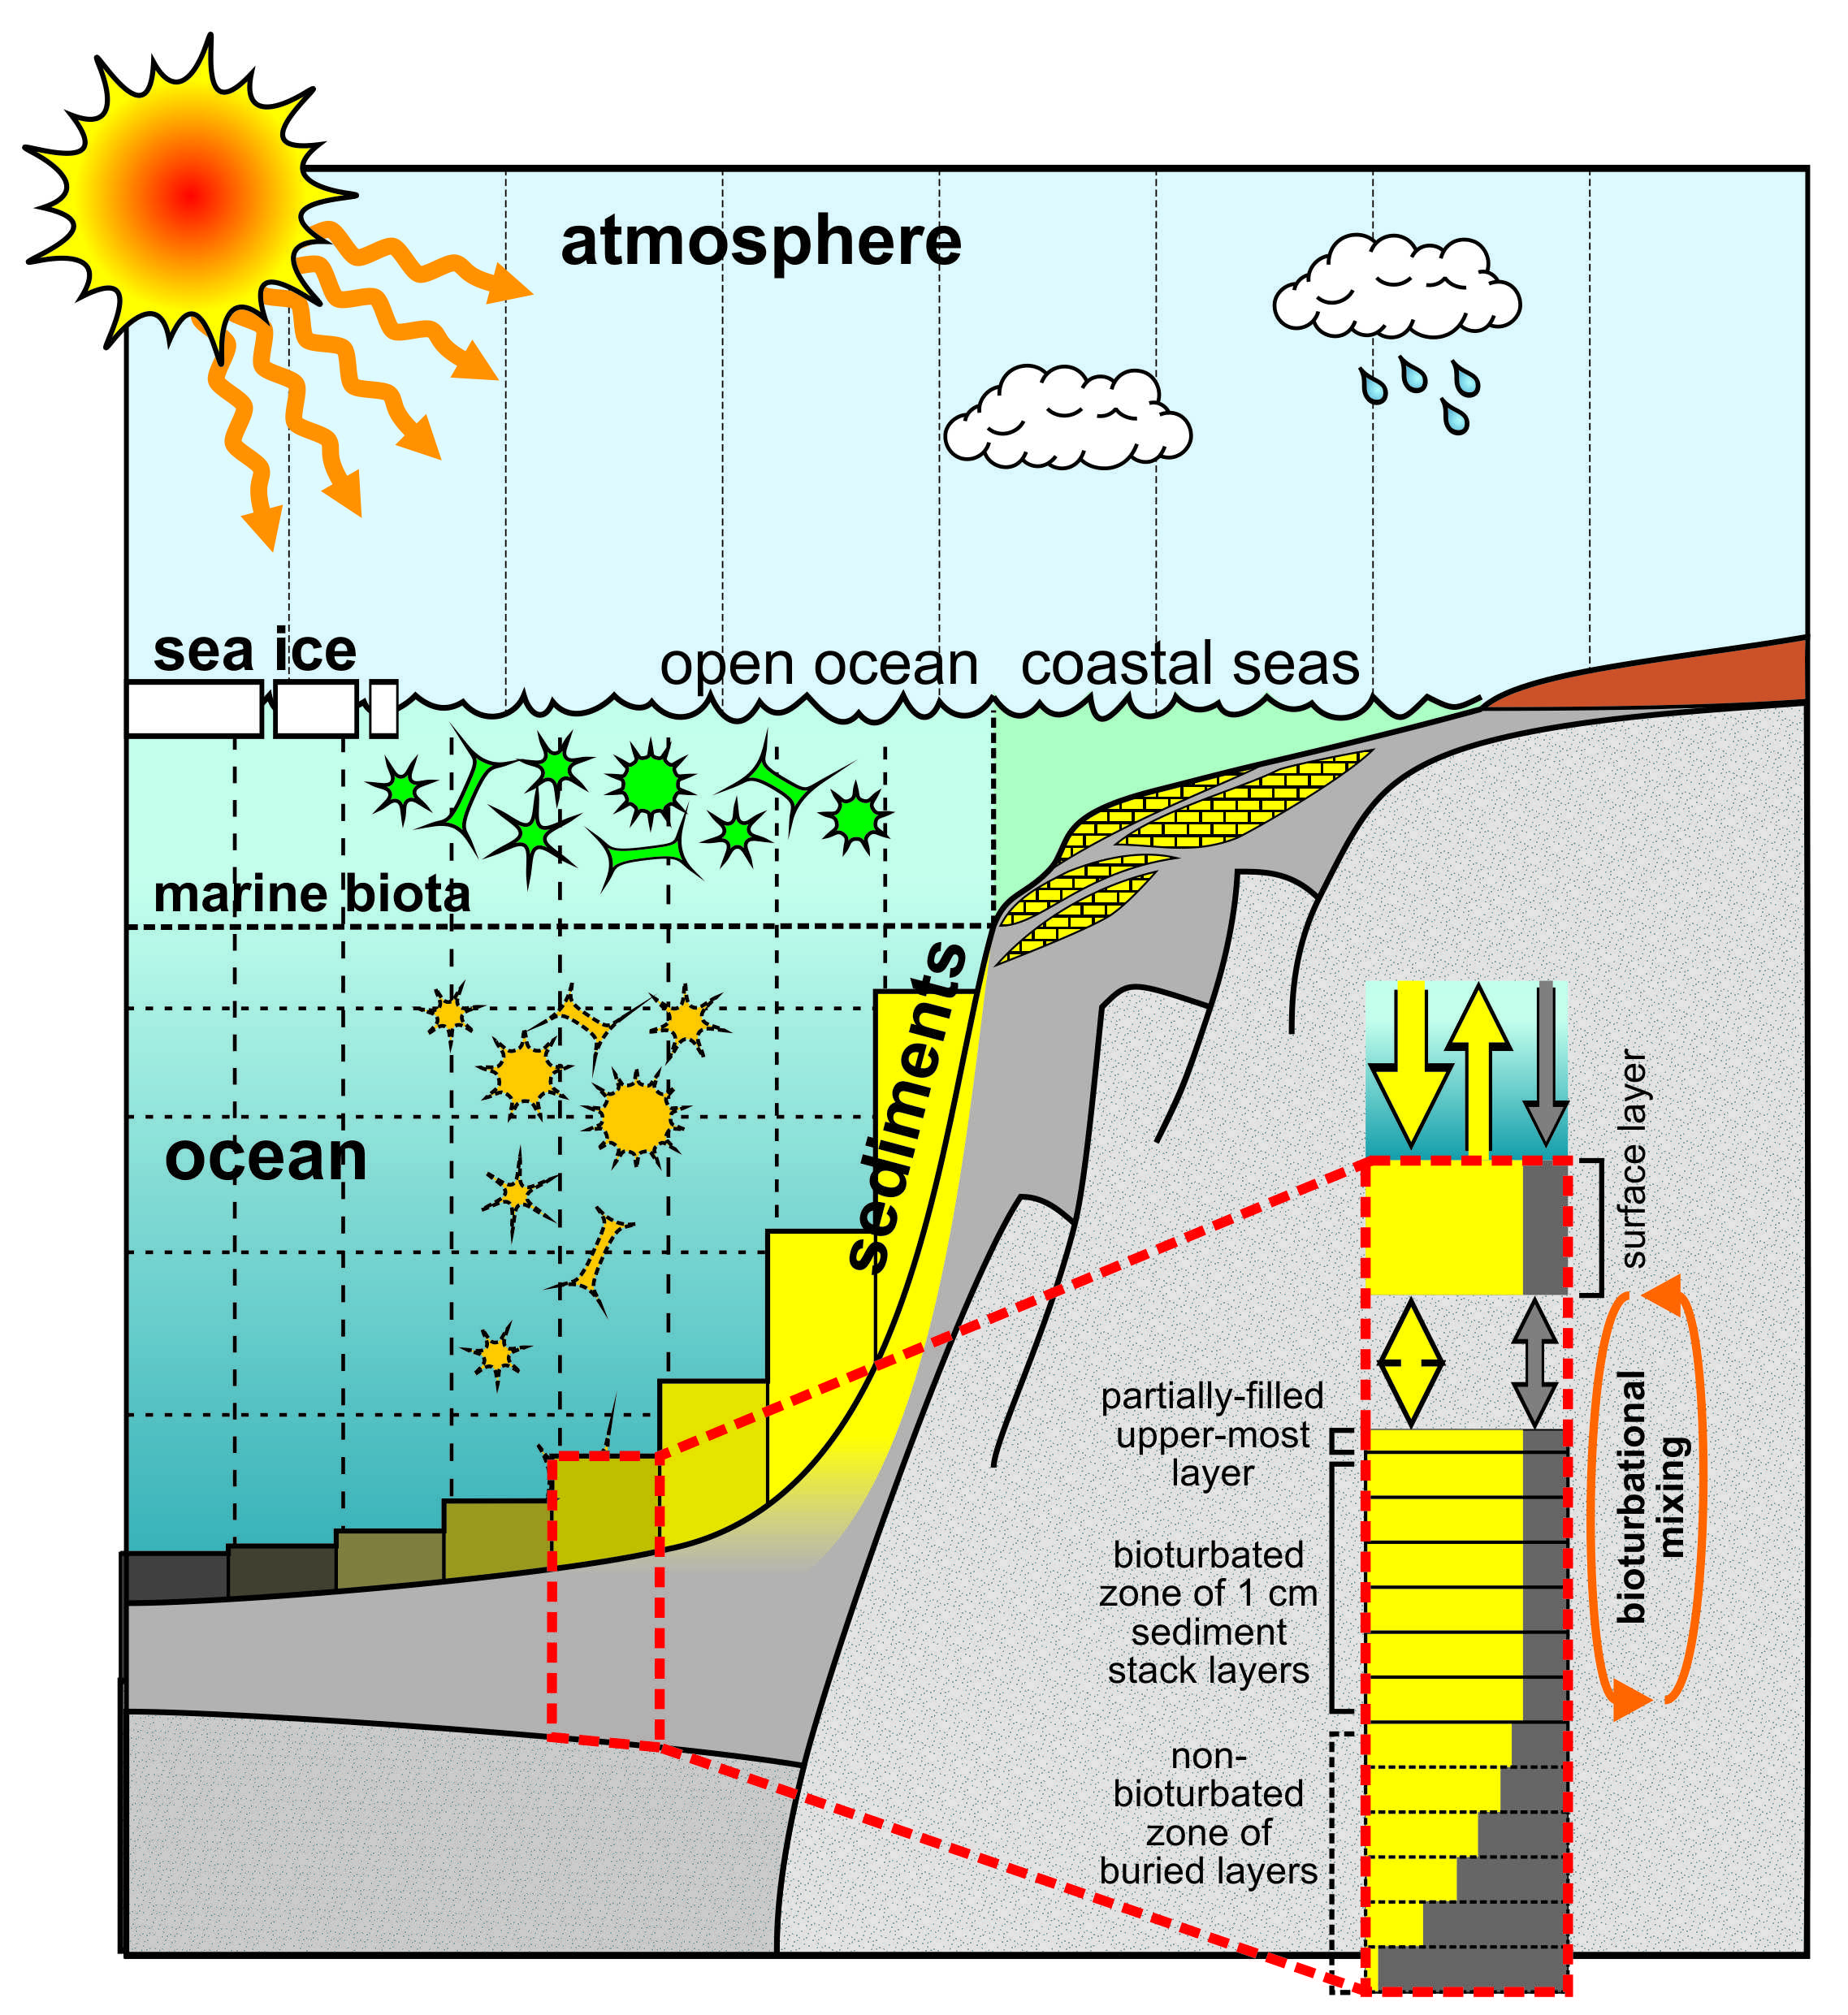
\includegraphics[width=0.5\textwidth]{sediments.jpg}
\caption{Schematic of \textbf{SEDGEM} sediment component.}
\label{fig:sediments}
\end{figure}

%------------------------------------------------
\vspace{1mm}
\noindent\rule{4cm}{0.1mm}
\vspace{2mm}
%------------------------------------------------

%------------------------------------------------
\newpage
%------------------------------------------------

\noindent Take the new model configuration for a test drive by running on from the \textit{re-start} experiment that you downloaded.

This is a steady-state climate+carbon cycle experiment that includes the deposition of \(CaCO_{3}\) in deep-sea sediments as well as the deposition of organic matter on continental shelves (plus a more minor contribution in deep-sea sediments), balanced by weathering (solute input to the ocean) plus volcanic \(CO_{2}\) out-gassing ... or at least as closely in balance as possible after 50,000 years. Try running ('briefly', but 100 years would not be too tedious for this faster configuration!) the following:

\vspace{-2mm}\small\begin{verbatim}
$ ./runmuffin.sh muffin.CBSR.fkl_pp51.BASESw
 LABS ch09.1.CTRL 100 231228.muffin.CBSR.fkl_pp51.BASESw.SPIN2
\end{verbatim}\normalsize\vspace{-2mm}

The \textit{user-config} \textsf{\footnotesize ch09.1.CTRL} is set up with the global carbon cycle configured as 'open' -- that is to say, that there is an input of carbon, alkalinity, and phosphorous to the ocean from weathering (plus carbon from volcanic out-gassing), and a loss due to preservation and burial of \(CaCO_{3}\) and organic matter in marine sediments. Depending on the state of ocean chemistry (and biology) and weathering, these two fluxes (input vs. output) do not have to balance, and hence ocean carbonate chemistry (and in turn, atmospheric \(pCO_{2}\)) can evolve with time. The \textit{spin-up} may not necessarily have the input and output fluxes absolutely perfectly balanced and hence before you run any experiments you might want to confirm whether the spin-up provided really is adequately 'spun-up'\footnote{i.e., you might plot some of the variables from the results of the \textit{spin-up}  experiment as a function of time and judge whether they are sufficiently converged or not.}. \textsf{\footnotesize ch09.1.CTRL} is hence configured to act as a control and quantify any residual flux imbalance and hence geochemical)(and climatic) 'drift'.

Note that a residual drift can be dealt with if it is relatively small and near linear via the use of a \uline{control experiment}, because any experiment you carry out will likely also incorporate (or be biased) by the same residual drift. Running a control gives you something to directly contrast  your experiment with and calculating the difference (e.g., a difference map or simple subtraction of global numbers) will give you the effect of whatever parameters you changed in the experiment but corrected for any drift. In previous exercises, you may have been a little lazy and created difference maps with respect to year 1 of an experiment -- strictly, they should have been created relative to the same year of a parallel control experiment, e.g., the results of a perturbation after 100 years should be contrasted with the year 100 results of the equivalent control.

%------------------------------------------------
\newpage
%------------------------------------------------

\noindent Before you look at any output from this experiment, you should note the following about this particular configuration and experiment:

\begin{enumerate}[noitemsep]
\vspace{1mm}
\item In the \textit{base-config} file naming convention -- the the '\textsf{\footnotesize S}' in \textsf{\footnotesize muffin.CBSR.fkl\_pp51.BASESw} specifies the use of a sediment model and the '\textsf{\footnotesize R}' a weathering module (see references should should have only just read!)\footnote{In addition to ocean and atmosphere biogeochemistry -- '\textsf{\footnotesize B}' and climate components (ocean, sea-ice, EMBM atmosphere) -- '\textsf{\footnotesize C}'.}
\vspace{1mm}
\item The '\textsf{\footnotesize w}' in \textsf{\footnotesize BASESw} specifies that a 'weathering' tracer has been included, which for simplicity, is dissolved silica. (See discussion later.)
\vspace{1mm}
\item We are running at a degraded (lower) \(18\times18\) resolution (but still \(16\) vertical levels in the ocean), and requiring fewer (twice as few in fact!) time-steps per year, for an overall approximately order-of-magnitude decrease in run-time as compared to a more standard \(36\times36\) resolution configuration of \textbf{muffin}. This is extremely helpful in being able to run \textbf{muffin} on geological time-scales but within a reasonable about of real time.
\vspace{1mm}
\item The configuration utilizes a conceptual/idealized continental configuration somewhat similar to as in the snowball Earth experiments.
\vspace{1mm}
\item Although this configuration could be regarded as a maximum complexity system, we are only going to initially look at this from the perspective of new output, and will reduce the complexity right down before we start to think about system behavior.
\vspace{1mm}
\item Data saving is set up for 2D only in \textbf{BIOGEM} (and not 3D), \textit{time-slices} only every 10000 years, and \textit{time-series} save points only every 100 years (all to minimize the size of the results files for loooooong experiment durations):
\vspace{-1mm}\small\begin{verbatim}
# force time-series saving @ 100 yr intervals
bg_par_infile_sig_name='save_timeseries_EVERY000100.dat'
# force 2D time-slice save only, and @ 10000 yr intervals
bg_ctrl_data_save_2d=.true.
bg_ctrl_data_save_3d=.false.
bg_par_infile_slice_name='save_timeslice_EVERY010000.dat'
\end{verbatim}\normalsize\vspace{-1mm}
You can return to the default saving you are used to by commenting out all these lines. Or you could change the name of the \textit{time-slice} and \textit{time-series} saving interval files, but making sure first the new file name exists (in directory: \textsf{\footnotesize genie-biogem/data/input} OR creating your own file there (and using that name).
\\Note that although a 100 year experiment will not yet have reached the first save point (with a mid-point time of 9999.5 years), \textbf{muffin} is configured to ALWAYS save you a final year \textit{time-slice}, regardless of whether your experiment duration ends up reaching a specific save point at run-end or not.
\vspace{1mm}
\item To date, the marine biochemical cycle of carbon and nutrients in muffin has included an 'implicit' alkalinity contribution (see Section 2.1 in: \textit{Ridgwell et al.} [2007]). In a fully open system with weathering and burial or organic carbon and nutrients, this becomes invalid. hence the inclusion in the \textit{user-config} of:
\vspace{-1mm}\small\begin{verbatim}
# *** BIOGEM ********************************************************
# remove organic matter associated (implicit nitrogen) alkalinity transformations
# => so we do not end up with spurious weathering ALK fluxes from kerogens 
#    (or spurious Corg burial related fluxes)
bg_par_bio_red_PON_ALK=0.0
\end{verbatim}\normalsize\vspace{-1mm}
%------------------------------------------------
\newpage
%------------------------------------------------
and in diagnosing \textbf{ROKGEM} parameter values:
\vspace{-1mm}\small\begin{verbatim}
# *** SEDGEM configuration ******************************************
# weathering diagnostic settings    
sg_par_sed_diag_P2ALK=0.0
\end{verbatim}\normalsize\vspace{-1mm}
\vspace{1mm}
\item Before we move on, a final instructive change from previously published configurations is:
\vspace{-1mm}\small\begin{verbatim}
# *** ROKGEM ********************************************************
# turn off atmospheric short circuit 
# (so CO2 is now removed from the atmosphere during weathering, 
#  and volcanic CO2 added to it)
# => to better diagnose weathering in BIOGEM output
rg_opt_short_circuit_atm=.false.
\end{verbatim}\normalsize\vspace{-1mm}
During weathering (of carbonate and silicate rocks), \(CO_{2}\) is assumed to dissolve in rainwater and reach with the calcium-bearing minerals. Later, in the ocean, when \(CaCO_{3}\) is precipitated and \(CO_{2}\) 'released'\footnote{Technically: made available for exchange with the atmosphere by a shift to lower pH.}, the \(CO_{2}\) originally removed from the atmosphere is regenerated/replaced. The 'short-circuit' is simple to assume this and not bother removing the one mol of \(CO_{2}\) in reaction with a mol of \(CaCO_{3}\) or \(CaSiO_{3}\). The \(CO_{2}\) consumption and removal from the atmosphere associated with silicate weathering is also not removed, on the basis that the alkalinity transported by rivers and added to the ocean will drive the draw-down if atmospheric \(pCO_{2}\) at that stage (rather than being removed up-front). Hence, in short-circuiting, the DIC transported to the ocean in rivers is equal to the weathering flux of carbon in \(CaCO_{3}\) plus the rate of \(CO_{2}\) out-gassing.

However, this only really 'works' if the system is in some sort of balance of weathering and precipitation and that alkalinity added to the surface ocean can fully equilibriate with the atmosphere ... which will not be the case during transient events (see Figure 3 in: \textit{Lord et al.} [2015]). Setting: \textsf{\footnotesize rg\_opt\_short\_circuit\_atm=.false.} instead tracks the \(CO_{2}\) fluxes explicitly and in full.
\\The potential implications of this will be a subject of a subsequent investigation ...
\\NOTE: A 'short-circuit' is fine if you are only looking at long-term weathering vs. sedimentation steady-states and not rapid carbon release driven transients.
\end{enumerate}

\vspace{1mm}
\noindent Other parameter settings will be introduced and explained as and when needed during this chapter.

%------------------------------------------------
\vspace{1mm}
\noindent\rule{4cm}{0.1mm}
\vspace{2mm}
%------------------------------------------------

%------------------------------------------------
\newpage
%------------------------------------------------

\section{Sediment model output}

There is a whole new set of additional outputs from this configuration of \textbf{muffin}, particularly sediment-specific output from the \textbf{SEDGEM} module and which is saved in the \textsf{\footnotesize sedgem} sub-directory of the main experiments results directory. Data saving differs from \textbf{BIOGEM} in that the composition of the sediments (and other diagnostics such as rain and dissolution fluxes) is saved only \uline{at the very end} of a model experiment (hence unlike \textbf{BIOGEM}, which by default saves a series of time-slices throughout the course of a model experiment). So if you kill a run before the very end (or the run crashes),  \uline{you will get no} (or little) \textbf{SEDGEM} output.

2D (e.g. surface sediment properties, fluxes, etc.) results can be found in  the \textsf{\footnotesize sedgem} sub-directory of your experiment directory  in a \textbf{netCDF} file called \textsf{\footnotesize fields\_sedgem\_2d.nc}. For example, the 2D distribution of \(wt\% CaCO_{3}\) –- which is the weight fraction of calcium carbonate (\(CaCO_{3}\)) in the surface sediments of the deep ocean (i.e., how much plankton carbonate shell material is there compared to other stuff in the mud at the bottom of the ocean), is saved in this \textbf{netCDF} file under a variable called: \textsf{\footnotesize sed\_CaCO3}. Note that there is some duplication of results saving, because a series of \textit{time-slices} of sediment composition are also saved in the 2D \textbf{BIOGEM} netCDF file \textsf{\footnotesize fields\_biogem\_2d.nc}. \textbf{BIOGEM} also saves a selection of \textit{time-series }of sediment properties -- \textsf{\footnotesize .res} files starting \textsf{\footnotesize biogem\_series\_sed}. For example, the \textit{time-series} file: \textsf{\footnotesize biogem\_series\_sed\_CaCO3.res} contains information about how the mean \(CaCO_{3}\) content of surface sediments (uppermost sediment layer) evolves with time. There are also \textit{time-series} file output that record the evolution of burial (and dissolution) fluxes as well as weathering -- all of which will be important for fully understanding system behavior.

As per with \textbf{BIOGEM} data saving, \textbf{SEDGEM} also saves a summary file of sediment fluxes and composition -- \textsf{\footnotesize seddiag\_misc\_DATA\_GLOBAL.res} as well as a parameter valiue summary for use in configuring \textbf{ROKGEM} (discussed later) -- \textsf{\footnotesize seddiag\_misc\_ROKGEM\_parameters.res}

%------------------------------------------------
\vspace{1mm}
\noindent\rule{4cm}{0.1mm}
\vspace{2mm}
%------------------------------------------------

\noindent The model also generates artificial sediment ‘cores’ (e.g. see: \textit{Ridgwell} [2007]) and hence what one might expect to see of your applied perturbations as recorded in a sediment core sand then recovered from the ocean floor(!) In the \textbf{SEDGEM} results sub-directory, there is a \textbf{netCDF} file which contains all the locations selected (if any) –- \textsf{\footnotesize sedcore.nc}. These are not really aligned with latitude as the \textbf{Panoply} display might suggest – the locations are in fact distributed from all over the ocean (\textbf{Panoply} is being fooled in order to display them together). In the \textbf{SEDGEM} 2D \textbf{netCDF} file, these locations are marked in the \textbf{netCDF} variable \textsf{\footnotesize grid\_mask\_sedcore}. The locations of these cores are stored in a a file containing a little ASCII ‘map’ of the ocean.
\vspace{1mm}

\begin{itemize}[noitemsep]
\vspace{1mm}
\item
If you are using a 'paleo' configuration of \textbf{muffin}, indicated by a parameter section in the \textit{base-config} file headed by something looking like:
\footnotesize\begin{verbatim}
# *******************************************************************
# GRID & BOUNDARY CONDITION CONFIGURATION
# *******************************************************************
# insert the automatically generated muffingen parameter list here
# *******************************************************************
##################################################################################
### cGENIE .config file parameter lines generated by muffingen v0.9.21 on: 220314 ###
\end{verbatim}\normalsize
then there will be a parameter line that direct muffin to look for \textbf{SEDGEM} configuration files in the respective \textsf{\footnotesize genie-paleo } directory, e.g.:
\vspace{-1mm}\small\begin{verbatim}
sg_par_pindir_name='../../cgenie.muffin/genie-paleo/fkl_pp51/'
\end{verbatim}\normalsize\vspace{-1mm}
\vspace{1mm}
\item Otherwise, the file lives in: \textsf{\footnotesize cgenie.muffin/genie-sedgem/data/input}
\end{itemize}
\vspace{1mm}
The filename is given by the parameter: \texttt{sg\_par\_sedcore\_save\_mask\_name}
\\Simply be editing (using the ASCII text editor) a '0.0' to a '1.0', you can get the model to generate and save a sediment ‘core’ at that particular (\textit{i,j}) location.

%------------------------------------------------
\vspace{1mm}
\noindent\rule{4cm}{0.1mm}
\vspace{2mm}
%------------------------------------------------

\noindent \textbf{netCDF} file \textsf{\footnotesize sedcore.nc } variables include:

\vspace{1mm}
\begin{itemize}[noitemsep]
\item \textsf{\footnotesize phys\_layer } –- sediment layer number (counting down).
\item \textsf{\footnotesize phys\_depth } -– (cumulative) depth below surface, measured from the sediment surface to the mid-point of each sediment layer (cm).
\item \textsf{\footnotesize th (cm) } -- thickness of each sediment layer (cm).
\item \textsf{\footnotesize age\_CaCO3 } -- the mean age of \(CaCO_{3}\) particles in a sediment layer.
\\Note that this will not be defined if there is no \(CaCO_{3}\) preserved.
\item \textsf{\footnotesize ... } then some alternative ways of assigning a chronology to a sediment core … (ignore) ...
\item \textsf{\footnotesize phys\_porosity  } -- sediment layer density (as if you cared!).
\item \textsf{\footnotesize sed\_POC } and \textsf{\footnotesize sed\_POC\_13C } -- mean organic matter content of each sediment layer and its \(\delta^{13} C\). But note: in this configuration no organic matter is preserved (hence all zeros for POC).
\item \textsf{\footnotesize sed\_CaCO3} and \textsf{\footnotesize sed\_CaCO3\_13C } -- mean \(CaCO_{3}\) content (wt\%) of each sediment layer and its \(\delta^{13} C\).
\item \textsf{\footnotesize sed\_det } and \textsf{\footnotesize sed\_ash } -- the wt\% detrital and ‘ash’ contents of a layer (ash is used as a conservative numerical sediment tracer in order to mark the depth of the start of the experiment).
\end{itemize}
\vspace{1mm}

\noindent Obviously – you could plot e.g. \(CaCO_{3}\) (or its \(\delta^{13}C\)) as a function of depth and/or age across and see how your carbon release experiment might be recorded in the marine geological record (e.g., how does this compare with observations across events such as the PETM?).

Note that the sediment cores reflect not only the material which has accumulated (or not, if it has dissolved …) during the course of your experiment, but also the material that accumulated during the spin-up. PLUS, whatever material the sediment core was initialized with to start with. For example, the large interval of initially 100\% detrital material at the base of the sediment core simply reflects the initialization of the sediment array in the model. Also note the ash ‘peak’ near the bottom of the stack (filled) sediment layers – this is a tracer to ‘tag’ the start of the model spin-up. If you look at the spin-up results (not your recent perturbation experiment) – the ash peak lies in a sediment layer with age equal to the total length of of the spin-up carried out. But why is there any ash deeper than the age corresponding to the start of the spin-up? How can it get there (i.e. what processes could move solid material deeper within the sediment column)?

%------------------------------------------------
\vspace{1mm}
\noindent\rule{4cm}{0.1mm}
\vspace{2mm}
%------------------------------------------------

\noindent If the provided experiment configuration does not specify the creation of any sediment cores -- go ahead and define some by editing file \textsf{\footnotesize fkl\_pp51.sedcoremask.dat} in: \textsf{\footnotesize cgenie.muffin/genie-paleo/fkl\_pp51} and flipping a '0.0' to a '1.0'. Then run a new experiment (copy-paste the \textit{user-config} and rename) for e.g., 100 years again as above and look for the additional (sediment core) output.

%------------------------------------------------
\newpage
%------------------------------------------------

Published examples of simulated marine sediment core output include (in order of publication date):
\begin{itemize}[noitemsep]
\item Ridgwell, A., Interpreting transient carbonate compensation depth changes by marine sediment core modeling, Paleoceanography 22, PA4102, doi:10.1029/2006PA001372 (2007).
\item Kirtland Turner, S., and A. Ridgwell, Recovering the true size of an Eocene hyperthermal from the marine sedimentary record, Paleoceanography (2013).
\item Jennions, S M., E. Thomas, D.N. Schmidt, D. Lunt, and A. Ridgwell, Changes in benthic ecosystems and ocean circulation in the Southeast Atlantic across Eocene Thermal Maximum 2, Paleoceanography DOI: 10.1002/2015PA002821 (2015).
\item Penman, D.E., S.Kirtland Turner, P. Sexton, R. Norris, A.J. Dickson, S. Boulila, A. Ridgwell, R.E. Zeebe, J. Zachos, A. Cameron, T. Westerhold, U. Röhl, IODP Expedition 342 Scientists, An abyssal carbonate compensation depth overshoot in the aftermath of the Palaeocene- Eocene Thermal Maximum, Nature Geoscience 9, doi:10.1038/NGEO2757 (2016).
\item (in the SI) Gutjahr, M., A. Ridgwell, P.F Sexton, E. Anagnostou, P.N. Pearson, H. Pälike, R.D. Norris, E. Thomas, and G.L. Foster, Very large release of mostly volcanic carbon during the Paleocene-Eocene Thermal Maximum Paleocene-Eocene Thermal Maximum, Nature 548, doi:10.1038/nature23646 (2017).
\item Fantle, M. S., and A. Ridgwell, Towards an understanding of the Ca isotopic signal related to ocean acidification and alkalinity overshoots in the rock record, Chemical Geology DOI: 10.1016/j.chemgeo.2020.119672 (2020).
\end{itemize}
and you might want to think about how you might make use of the \textit{sedcore} output in light of these papers.

%------------------------------------------------
\newpage
%------------------------------------------------

\section{Quantifying how long is the 'long tail' of CO$_{2}$}

The 'full' geological carbon cycle is complex ... we'll pick it apart soon ... but you may as well have a quick 'play'. Regardless, highly idealized perturbations are the way to go first. Specifically -- an illustrative experiment which has a parallel to experiments you have conducted previously, is to add a pulse \(CO_{2}\) release to the atmosphere and track the consequences for atmospheric p\(CO_{2}\) and ocean chemistry (particularly ‘alkalinity’), and now also e.g. deep sea sediments. 

\vspace{1mm}
In the \textsf{\footnotesize ch09.3.EXPT} \textit{user-config}, the lines:
\vspace{-2mm}\small\begin{verbatim}
bg_par_forcing_name='pyyyyz.FpCO2_Fp13CO2'
bg_par_atm_force_scale_val_3=8.3333e+016
bg_par_atm_force_scale_val_4=-15.0
\end{verbatim}\normalsize\vspace{-2mm}
specify the release of \(CO_{2}\) to the atmosphere at a rate of \(0.1 PgC yr^{-1}\) with an isotopic composition of \(-15\)\permille -- appropriate for a volcanic-related geological source. The lines:
\vspace{-2mm}\small\begin{verbatim}
bg_par_atm_force_scale_time_3=10000.0
bg_par_atm_force_scale_time_4=10000.0
\end{verbatim}\normalsize\vspace{-2mm}
then specify that this input (and isotopic composition) continues over 10,000 years.

\vspace{1mm}
Unless you wish to run an experiment for 10,000 years or more (yawn!!), you might want to reduce the interval emissions are over (changing both parameter values equally) as well as increasing the emissions rate (as you did in earlier exercises). You could also consider isotopic compositions of \(-27\)\permille -- appropriate for a fossil fuel carbon source, or methane derived carbon (e.g., as from hydrates) which would be more like \(-60\)\permille and create a more exciting carbon isotopic perturbation to watch. For example, perhaps something like:
\vspace{-2mm}\small\begin{verbatim}
# specify forcings -- 5,000 PgC @ -60 o/oo over 100 yr
bg_par_forcing_name="pyyyyz.FpCO2_Fp13CO2"
bg_par_atm_force_scale_val_3=8.3333e+013
bg_par_atm_force_scale_val_4=-60.0
bg_par_atm_force_scale_time_3=100.0
bg_par_atm_force_scale_time_4=100.0
\end{verbatim}\normalsize\vspace{-2mm}
would be like a slightly super-charged anthropogenic experiment\footnote{50 PgC per year for 100 years, as opposed to the current ca. 10 PgC per year.} and with more a more pronounced isotopic fingerprint. Or configure the same emissions as you might have explored before\footnote{(e.g., 1000 PgC over 1 year)} .

\vspace{1mm}
Run the model for as long as you dare (or can be bothered) – 1,000 or 2,000 years might be just enough  to start to see impacts on deep-sea sediments, but 10,000 years or more would be much better. (You can always submit this to the cluster queue and get on with something else.) FYI: 10,000 years is going to take something like an hour ... if you are lucky ...

Remember the earlier comment earlier in the chapter about the frequency of output saving -- you may well want at the very least, more frequent \textit{time-series} saving\footnote{Comment out to obtain default saving intervals, or change a save interval definition file with a shorter regular spacing in time.}.

Plot the time-series of e.g. atmospheric \(pCO_{2}\) and compare to the (much shorter experiments) you have carried out before with a simple ocean+atmosphere only system. Compare how quickly atmospheric \(pCO_{2}\) decays compared to previously \textbf{muffin} publications (e.g., \textit{Ridgwell and Hargreaves} [2007]) or other models (e.g. \textit{Archer et al.} [2009]) and  how the sediments respond (e.g. the time-series of sediment \(CaCO_{3}\) content).

%------------------------------------------------
\newpage
%------------------------------------------------

\noindent BE CAREFUL -- if you have previously edited the \textit{forcing} \textsf{\footnotesize  pyyyyz.FpCO2\_Fp13CO2}, you are going to need to return whatever files you edited back to their original state.
\small\begin{enumerate}[noitemsep]
\vspace{1mm}
\item From \textsf{\footnotesize genie-main}, \texttt{\$ make cleanall}
\vspace{1mm}
\item Then head up a directory level (\texttt{cd ..}) to \textsf{\footnotesize cgenie.muffin}
\vspace{1mm}
\item Type: \texttt{\$ git status -uno}
\vspace{1mm}
\\You should see a list of all files originally cloned from GitHub) that have changed, e.g.:
\vspace{-1mm}\begin{verbatim}
modified:   genie-forcings/pyyyyz.FpCO2_Fp13CO2/biogem_force_flux_atm_pCO2_sig.dat
\end{verbatim}\vspace{-1mm}
(Note that files you create are not listed. TO see those, type: \texttt{\$ git status})
\vspace{1mm}
\item To restore the state of any file that you might have edited, \texttt{git checkout} that file out, e.g.:
\vspace{-1mm}\begin{verbatim}
$ git checkout genie-forcings/pyyyyz.FpCO2_Fp13CO2/biogem_force_flux_atm_pCO2_sig.dat
\end{verbatim}\vspace{-1mm}
\end{enumerate}\normalsize

%------------------------------------------------
\vspace{1mm}
\noindent\rule{4cm}{0.1mm}
\vspace{2mm}
%------------------------------------------------

\noindent DON'T FORGET -- Did you remember to run a control experiment? The same experiment\footnote{(Just copy-paste and then rename \textsf{\footnotesize ch09.3.EXPT} -> \textsf{\footnotesize ch09.3.CTRL} or similar.}  you have probably just pressed \textsf{\footnotesize return} on, but with the rate of carbon emissions set to zero (no other changes ... run for the same experiment duration ...).

%------------------------------------------------
\vspace{1mm}
\noindent\rule{4cm}{0.1mm}
\vspace{2mm}
%------------------------------------------------

\noindent To properly (quantitatively) appreciate the role of ocean-sediment interaction (and weathering) and controlling atmospheric \(pCO_{2}\), you need to contrast these experiments with as similar a model configuration as possible -- for instance, one that is identical excepting having no sediments (or weathering). 

You can achieve this quite simply: create (/copy-rename) a new \textit{user-config} based on \textsf{\footnotesize ch09.3.EXPT} and edit the lines\footnote{You do not have to edit the comment line (\#) but it will help you remember what you have done.}:
\vspace{-1mm}\small\begin{verbatim}
# set an 'OPEN' system
bg_ctrl_force_sed_closedsystem=.false.
\end{verbatim}\normalsize\vspace{-1mm}
changing it to:
\vspace{-1mm}\small\begin{verbatim}
# set a 'CLOSED' system
bg_ctrl_force_sed_closedsystem=.true.
# automatically seed all weathering fluxes as non-zero
rg_ctrl_force_sed_closedsystem=.TRUE.
\end{verbatim}\normalsize\vspace{-1mm}

\noindent What this  does is to force the model to always maintain an exact balance between the preservation and burial in marine sediments of \(CaCO_{3}\) and organic matter (both carbon and nutrients), with the supply of solutes derived from the weathering of \(CaCO_{3}\), \(CaSiO_{3}\), organic matter, and apatite (for phosphate) on land, plus volcanic out-gassing. Because no excess or deficit of weathering vs. sedimentation is allowed to occur, no changes in ocean chemistry (other than by air-sea gas exchange) occur. This configuration hence acts (geochemically and dynamically) exactly the same way as a configuration without any sediments or weathering being present (and as used previously). 

However, for this setting to work properly, you do need to flip 'short-circuiting' back on to ensure that \(CO_{2}\) is not being removed and hence being drained from the atmosphere, and hence set: \texttt{rg\_opt\_short\_circuit\_atm=.false.}

%------------------------------------------------
\newpage
%------------------------------------------------

By comparing the two experiments (with and without a 'closed system', and also both with the control): can you deduce the effect of the sediment and weathering interactions and feedbacks in modulating (accelerating or decelerating) atmospheric \(pCO_{2}\) decline?\footnote{e.g. you could compare the \(pCO_{2}\) time-series of the 2 different experiments, or create anomalies from both with respect to the control, and then contrast.}

Also view the sediment distribution (of \(CaCO_{3}\)): what are the impacts on sediment composition in the case of an experiment configured with an ‘open’ system (vs. a 'closed' system)? Here, the time-series file of mean global sediment composition \textsf{\footnotesize biogem\_series\_sed\_CaCO3.res} (in units of: \(wt\%\:CaCO_{3}\)) may help illustrate what is going on here.
Note that the way the ‘closed’ system is constructed; a response of the sediments is predicted and saved in the output, even though it is not allowed to affect chemistry or atmospheric p\(CO_{2}\).

%------------------------------------------------
\vspace{1mm}
\noindent\rule{4cm}{0.1mm}
\vspace{2mm}
%------------------------------------------------

\noindent To recap -- you are aiming to run a \(CO_{2}\) emissions experiment using a \textbf{muffin} configuration including variable weathering and sedimentation (\textsf{\footnotesize ch09.3.EXPT}) with a version/copy that you have edited to create a 'closed' ocean-atmosphere system, with no ocean-sediment or weathering feedbacks on atmospheric \(CO_{2}\). Ideally, you would also run a PAIR (not just one!) of control experiments -- one for each of 'open' and 'closed' configurations and each with no \(CO_{2}\) emissions specified. (A total of 4 experiments.)

%------------------------------------------------
\newpage
%------------------------------------------------

\section{Sediments of the modern Earth}

Having had a quick 'play' with the system, we should return -- albeit briefly -- to reality and critically and quantitatively assess to what degree \textbf{muffin}  provides an adequate representation of the interaction between ocean chemistry and sediment composition (e.g., in \(CaCO_{3}\) buffering of \(CO_{2}\) release and 'carbonate compensation'). Key to this, is contrasting  model output against observational-based data. Such an approach is presented in \textit{Ridgwell and Hargreaves} [2007]. Note that the following experiments, for which you are NOT provided \textit{restarts} for, take a few days to run and you might consider getting these\footnote{Although the 2nd-stage \textit{spin-up} will require the first stage one to complete.} on the cluster queue and work on the next section (or more experiments from the previous one) while they run.

\vspace{1mm}
The required \textit{base-} and \textit{user-config} files are both provided as part of the \textbf{muffin} code release:

\begin{itemize}[noitemsep]
\vspace{1mm}
\item \textsf{\footnotesize muffin.CBSR.p\_worbe2.BASES} -- the \textit{base-config} file, including \textbf{SEDGEM} (the '\textsf{\footnotesize S}' in '\textsf{\footnotesize CBSR}' and \textbf{ROKGEM} -- '\textsf{\footnotesize R}') modules.
\vspace{1mm}
\item \textsf{\footnotesize muffin.CBSR.p\_worbe2.BASES.RidgwellHargreaves1997\_S36x36.SPIN1} -- the \textit{user-config} for the 1st stage (20 kyr long) \textit{spin-up} described in \textit{Ridgwell and Hargreaves} [2007]. This file lives in the \textsf{\footnotesize EXAMPLES} sub-directory of \textsf{\footnotesize genie-userconfigs}.
\end{itemize}

This can then be run:
\vspace{-1mm}\small\begin{verbatim}
./runmuffin.sh muffin.CBSR.p\_worbe2.BASES EXAMPLES
   muffin.CBSR.p_worbe2.BASES.RidgwellHargreaves1997_S36x36.SPIN1 20000
\end{verbatim}\normalsize\vspace{-1mm}

Read the paper and consider the plotted core-top sediment composition data-set (and ideally, \uline{read the associated cited papers by David Archer}). Does the model get the broad patterns right (is it more right than wrong, or more wrong than right)? Do you think the model-data misfits might be important? How so?

%------------------------------------------------
\vspace{1mm}
\noindent\rule{4cm}{0.1mm}
\vspace{2mm}
%------------------------------------------------

\noindent A \textit{user-config} for the second-stage spin-up as described in \textit{Ridgwell and Hargreaves} [2007] is also provided:
\begin{itemize}[noitemsep]
\vspace{1mm}
\item \textsf{\footnotesize muffin.CBSR.p\_worbe2.BASES.RidgwellHargreaves1997\_S36x36.SPIN2} is the 2nd-stage, 50 kyr \textit{spin-up} that uses \textsf{\footnotesize muffin.CBSR.p\_worbe2.BASES.RidgwellHargreaves1997\_S36x36.SPIN1} as a \textit{re-start}.
\end{itemize}
\vspace{1mm}
and can be run:
\vspace{-1mm}\small\begin{verbatim}
./runmuffin.sh muffin.CBSR.p\_worbe2.BASES EXAMPLES
   muffin.CBSR.p_worbe2.BASES.RidgwellHargreaves1997_S36x36.SPIN2 50000
   muffin.CBSR.p_worbe2.BASES.RidgwellHargreaves1997_S36x36.SPIN1
\end{verbatim}\normalsize\vspace{-1mm}

Having run the second spin-up, which now includes a full bioturbated sediment depth of \(CaCO_{3}\) that can potentially be reacted with \(CO_{2}\) added to the system (see: \textit{Ridgwell and Hargreaves} [2007] and also \textit{Ridgwell} [2007]), you could try and perturbation experiment. All you need to do, is take \textsf{\footnotesize muffin.CBSR.p\_worbe2.BASES.RidgwellHargreaves1997\_S36x36.SPIN2}, copy-and-rename as per usual, and then change the \textit{forcing}.

%------------------------------------------------
\newpage
%------------------------------------------------

The current \textit{forcing} is:
\vspace{-1mm}\small\begin{verbatim}
# specify forcings -- ONLY apply a non-carbonate (detrital) flux (to the sediments)
bg_par_forcing_name="worbe2.detplusopalSED"
\end{verbatim}\normalsize\vspace{-1mm}
This specifies a 'detrital' field -- basically the rate of accumulation of non carbonate solids in the sediments (see: \textit{Ridgwell and Hargreaves} [2007] and references there-in). You need to retain this specified detrital flux forcing, but add a \(CO_{2}\) one to the atmosphere. One is provided in the \textit{forcings} directory\footnote{\textsf{\footnotesize worbe2.FpCO2\_Fp13CO2.detplusopalSED}}, but more instructive is to adapt the current one. To do this:
\begin{enumerate}[noitemsep]
\vspace{1mm}
\item Copy-and-rename the forcing folder that is currently pointed to -- \textsf{\footnotesize worbe2.detplusopalSED}.
\vspace{1mm}
\item Find a previous experiment where you released \(CO_{2}\) to the atmosphere, and find the \textit{forcing} folder used for that\footnote{It may well have been called something like: \textsf{\footnotesize pyyyyz.FpCO2\_Fp13CO2}}.
\vspace{1mm}
\item Three files in the \(CO_{2}\) emissions \textit{forcing} folder together define a \(CO_{2}\) flux is to be used:
\\\textsf{\footnotesize configure\_forcings\_atm.dat}
\\\textsf{\footnotesize biogem\_force\_flux\_atm\_pCO2\_sig.dat}
\\\textsf{\footnotesize biogem\_force\_flux\_atm\_pCO2\_13C\_sig.dat}
\\(If you have forgotten what these are/do -- refer back to the ocean circulation and/or fossil fuel emissions chapters.)
\\Simply copy these 3 files into your new \textit{forcing} folder.
\vspace{1mm}
\item Change the name of the forcing in your \textit{user-config}, and scale the \(CO_{2}\) flux as per you did earlier, e.g., adding:
\vspace{-1mm}\small\begin{verbatim}
bg_par_atm_force_scale_val_3=8.3333e+013
bg_par_atm_force_scale_val_4=-27.0
\end{verbatim}\normalsize\vspace{-1mm}
This would give you just \(1 PgC yr^{-1}\) (at \(-27\)\permille), so you need to adjust this (refer to earlier in this chapter, and to earlier chapters).
\end{enumerate}

%------------------------------------------------
\vspace{1mm}
\noindent\rule{4cm}{0.1mm}
\vspace{2mm}
%------------------------------------------------

\noindent How the 2nd stage spin-up is derived from the results of the first and how either \textit{user-config} is constructed in the first place, we will look at in the next section. For now, just note the following about the two provided experiment configurations:

\vspace{1mm}

\begin{itemize}[noitemsep]
\vspace{1mm}
\item SPIN1 is 'closed':
\vspace{-1mm}\small\begin{verbatim}
rg_ctrl_force_sed_closedsystem=.TRUE.
\end{verbatim}\normalsize\vspace{-1mm}
\vspace{1mm}
\item SPIN1 sets a parameter value that is not used in the experiment itself, but informs the calculation of the \textbf{ROKGEM} parameters for use in SPIN2:
\vspace{-1mm}\small\begin{verbatim}
sg_par_sed_diag_fracSiweath=0.0
\end{verbatim}\normalsize\vspace{-1mm}
\vspace{1mm}
\item SPIN2 has a section of parameters that were automatically-generated -- the section starting:
\vspace{-1mm}\small\begin{verbatim}
 # --- ROKGEM USER-CONFIG --------
 # NOTE: automatically generated by SEDGEM
\end{verbatim}\normalsize\vspace{-1mm}
\end{itemize}

%------------------------------------------------
\newpage
%------------------------------------------------

\section{The marine geology of fake worlds}

You can configure any of your previous fake worlds, or generate new ones, to have a full geologic carbon cycle including deposition of \(CaCO_{3}\) in marine sediments and weathering on land.

In order to generate the requisite \textbf{SEDGEM} configuration files, you need the following settings in your \textbf{muffingen} configuration file:

\begin{itemize}[noitemsep]
\vspace{1mm}
\item \texttt{opt\_makeseds=true;} --  requests that \textbf{SEDGEM} files are generated.
\vspace{1mm}
\item \texttt{par\_sedsopt=2;} -- requests that a randomized bathymetry is generated. This is needed because fake worlds have by default, a flat bathymetry.
\\Instead, if you 'draw' a non-uniform bathymetry, you would set:
\\ \texttt{par\_sedsopt=0;} -- requests that the ocean depth levels ('k1' file') are used to inform the ocean floor depth assumed by \textbf{SEDGEM}.
\\(Option \texttt{1} is most commonly used in conjunction with a GCM-derived continental configuration.)
\end{itemize}

\vspace{1mm}
So, if you define continents in your fake world, but do not change the bathymetry in \textbf{muffingen}, \texttt{par\_sedsopt} option \texttt{2} will give you a randomized distribution of sediment depths (used in the \(CaCO_{3}\) solubility pressure calculation only). Selecting option \texttt{0} will simply translate your chosen \textbf{muffingen} ocean depths into \textbf{SEDGEM} depths. Note that you can still have a flat bottom to the ocean (no variation in ocean floor depth) and choose option \texttt{0}.

If you define a specific bathymetry by hand (e.g. draw in ocean ridges), you probably do not want it over-written (by a random \textbf{SEDGEM} depth pattern) and hence you should chose option \texttt{0}.

For speed of running model experiments, it is recommended that you generate your \textbf{muffingen} \textbf{muffin} configurations at the lowest reasonable resolution -- \(18\times18\times8\) would be suitable -- \(18\times18\) resolution in lon vs. lat, and \(8\) levels in the ocean. (You could try pushing this a little further and more extreme, e.g. \(12\times12\times8\).) Note that when you create your \textit{base-config}, you should use the template:
\vspace{1mm}
\\\textsf{\footnotesize CONFIG\_template\_08lvl\_R07.config}
\vspace{1mm}
\\(for the 8-level ocean, rather than \textsf{\footnotesize CONFIG\_template\_16lvl\_R07.config } which is designed for 16-ocean level configurations).

Once you have copy-pasted the configuration output of \textbf{muffingen} into the template \textit{base-config} file (and suitably renamed it), you need to enable the geologic carbon cycle modules (\textbf{SEDGEM} and \textbf{ROCKGEM}). At the top of the \textit{base-config} file, ensure that the following are set:
\vspace{-1mm}\small\begin{verbatim}
ma_flag_sedgem=.TRUE.
ma_flag_rokgem=.TRUE.
\end{verbatim}\normalsize\vspace{-1mm}
And then, further down and under the heading:
\vspace{-1mm}\small\begin{verbatim}
# TRACER CONFIGURATION
\end{verbatim}\normalsize\vspace{-1mm}
you need to define how many 'tracers' in the ocean, what they are, and any initial values that differ from modern defaults. Plus, whatever atmospheric and sediment tracers you want (plus default values in the atmosphere). Simplest at this point is to copy-paste from an existing \textit{base-config}, such as:
\vspace{1mm}
\\\textsf{\footnotesize cgenie.eb\_go\_gs\_ac\_bg\_sg\_rg.worbe2.BASE}
\vspace{1mm}
\\(which is the \textit{base-config} used in \textit{Ridgwell and Hargreaves} [2007]).

\vspace{1mm}
As for a suitable \textit{user-config} ...

... you could take the \textit{user-config} from \textit{Colbourn et al.} [2013] (itself a modification of Ridgwell and Hargreaves [2007]) -- available as part of the \textbf{muffin} code release, as file:
\vspace{1mm}
\\\textsf{\footnotesize EXAMPLE.worbe2.Colbournetal2013.CTRL } (\textsf{\footnotesize genie-userconfigs } sub-directory)
\vspace{1mm}
\\Then generalize this according to the paleo sediment configuration used in \textit{Ridgwell and Schmidt} [2010] (file: \textsf{\footnotesize EXAMPLE.p0055c.RidgwellSchmidt2010.SPIN1 } in the \textsf{\footnotesize genie-userconfigs } sub-directory) (i.e. making \(CaCO_{3}/POC\) export invariant, adding a fixed detrital flux to the sediments).

Cutting the lines down to the bare minimum (excepting comments pertaining to new/altered lines), a suitable \textit{user-config} then looks like:

\scriptsize\begin{verbatim}
# --- CLIMATE --------------------------------------------------
# enable CO2 climate feedback
ea_36=y
# --- BIOLOGICAL NEW PRODUCTION --------------------------------
bg_par_bio_k0_PO4=1.9582242E-06
bg_par_bio_c0_PO4=2.1989611E-07
# --- ORGANIC MATTER EXPORT RATIOS -----------------------------
bg_par_bio_red_DOMfrac=0.66
# --- INORGANIC MATTER EXPORT RATIOS ---------------------------
# set fixed export CaCO3 as a proportion of particulate organic matter
bg_par_bio_red_POC_CaCO3=0.200
bg_par_bio_red_POC_CaCO3_pP=0.0
# --- REMINERALIZATION -----------------------------------------
bg_par_bio_remin_DOMlifetime=0.5
bg_par_bio_remin_POC_frac2=6.4591110E-02
bg_par_bio_remin_POC_eL1=550.5195
bg_par_bio_remin_POC_eL2=1000000.0
bg_par_bio_remin_CaCO3_frac2=0.468
bg_par_bio_remin_CaCO3_eL1=1083.486
bg_par_bio_remin_CaCO3_eL2=1000000.0
# --- SEDIMENTS ------------------------------------------------
# sediment diagenesis options
sg_par_sed_diagen_CaCO3opt="ridgwell2001lookup"
sg_ctrl_sed_bioturb=.true.
sg_ctrl_sed_bioturb_Archer=.false.
sg_par_n_sed_mix=20
sg_par_sed_mix_k_sur_max=0.15
sg_par_sed_mix_k_sur_min=0.15
# additional detrital flux (g cm-2 kyr-1)
sg_par_sed_fdet=0.180
# --- WEATHERING -----------------------------------------------
# set a 'OPEN' system
bg_ctrl_force_sed_closedsystem=.false.
# set CaCO3_weathering-temperature feedback
rg_opt_weather_T_Ca=.TRUE.
# set CaSiO3_weathering-temperature feedback
rg_opt_weather_T_Si=.TRUE.
# weathering reference mean global land surface temperature (C)
rg_par_ref_T0=8.48
#CO2 outgassing rate (mol C yr-1)
rg_par_outgas_CO2=5.59E+12
# global silicate weathering rate (mol Ca2+ yr-1)
rg_par_weather_CaSiO3=5.59E+12
# global carbonate weathering rate (mol Ca2+ yr-1)
rg_par_weather_CaCO3=5.59E+12
# d13C
rg_par_outgas_CO2_d13C=-6.0
rg_par_weather_CaCO3_d13C=12.8
# --- DATA SAVING ----------------------------------------------
bg_par_data_save_level=4
bg_ctrl_debug_lvl0=.true.
ma_debug_loop=1
# --- END ------------------------------------------------------
\end{verbatim}\normalsize

Here, the reference temperature against which  the rate of weathering is modified for higher/lower temperatures, is set for a modern-like continental configuration:
\vspace{-1mm}\small\begin{verbatim}
# weathering reference mean global land surface temperature (C)
rg_par_ref_T0=8.48
\end{verbatim}\normalsize\vspace{-1mm}
If left un-changed, then the negative silicate weathering feedback will operate on atmospheric \(CO_{2}\) -- letting it accumulate, or removing it, until the reference temperature is achieved. If instead, you want to achieve a specific atmospheric \(CO_{2}\) at steady state, you need to know the relevant mean global land surface temperature. To determine this -- first run \textbf{muffin} with a prescribed atmospheric \(CO_{2}\) value, e.g. by adding:
\vspace{-1mm}\small\begin{verbatim}
# --- FORCINGS -------------------------------------------------
# specify forcings
bg_par_forcing_name="pyyyyz.RpCO2_Rp13CO2"
bg_par_atm_force_scale_val_3=278.0E-06
bg_par_atm_force_scale_val_4=-6.5
\end{verbatim}\normalsize\vspace{-1mm}
(or some other value of \(CO_{2}\)) to your \textit{user-config}. Running the model for about 1000 years should be more than enough to achieve a near steady-state of surface climate, allowing to read off the mean global surface air temperature over land (BIOGEM file \textsf{\footnotesize biogem\_series\_misc\_SLT.res}), and set the reference temperature to this value. You can then run an experiment without a prescribed atmospheric \(CO_{2}\) forcing, now knowing that the silicate weathering feedback will always act to restore atmospheric \(CO_{2}\) back to that value.

\vspace{1mm}
\noindent\rule{4cm}{0.5pt}
\vspace{2mm}

\noindent Despite the low grid resolution, this is still  going to take a l o n g time for particularly much to happen and you could probably do with some (numerical) 'help'. You can accelerate the run-time of \textbf{muffin} in calculating the balance between weathering and sedimentation, a-la \textit{Lord et al.} [2015]. To do this, you need to add a new section of parameter choices to the \textit{user-config} file:
\vspace{-1mm}\small\begin{verbatim}
# --- GEOCHEM ACCELERATION -------------------------------------
gl_ctrl_update_pCO2=.true.
ma_gem_notyr_min=10
ma_gem_notyr_max=10
ma_gem_yr_min=90
ma_gem_yr_max=90
ma_gem_dyr=0
ma_gem_adapt_auto=.false.
\end{verbatim}\normalsize\vspace{-1mm}
Here, this specifies that you would like to spend only \(10\) years of full updating of the model for each \(90\) years spent in an accelerated calculation which treats the entire ocean as if it were a single geochemical reservoir (see: \textit{Lord et al.} [2015]) -- an almost \(10:1\) acceleration and reduction in experiment run-time. (But note that the ocean circulation and ocean carbon and nutrient cycles will appear to be taking longer to come to equilibrium because they are only being fully updated \(10\) years in every \(100\).

Note that this acceleration is good for spin-ups and determining equilibrium weathering-sedimentation states, but not so useful for transient \(CO_{2}\) changes (see in \textit{Lord et al.} [2015] for how a less acceleration and adaptive setup had to be used). Similarly, acceleration is not so useful for varying orbits experiments.

\vspace{1mm}
\noindent\rule{4cm}{0.5pt}
\vspace{2mm}

\noindent A couple of different possible experimental investigations follow.\footnote{Note that in using the given \textit{user-config} settings, steady state is only reach after several 100 kyr (which is going to take a while, even at low resolution and with acceleration). Regardless of your assumptions regarding sea-floor bathymetry, you should find that atmospheric \(CO_{2}\) always reaches the same value.
}
\begin{enumerate}[noitemsep]

\vspace{1mm}
\item Firstly, you could simply test what happens if there is no sediment surface depth variability as compared to a configuration with depth (pressure) variability in sediment surface depth (and one that follows a modern-like distribution of depth vs. area). The science question would be something like -- how important is a distribution of ocean depths to setting the steady state alkalinity (or saturation) of the ocean? Or: in having an appreciable amount of shallower sea-floor where \(CaCO_{3}\) will be preserved and buried much more readily -- how much less saturated must the ocean as a whole become in order to balance weathering and sedimentation?
\\F or this, you'll need 2 \textbf{muffingen} configurations, each with the same continental configuration, but one generated with random sediment depths, and one with a uniform depth.
\\Simplest, but more tedious, is to run \textbf{muffingen} twice, with your  configuration settings files differing only in the value of \texttt{par\_sedsopt}. However, faster is to generate one configuration using the configuration template \textsf{\footnotesize EXAMPLE\_BLANK.m}, and then generate a 2nd one, using the 'k1' file generated by the first \textbf{muffingen} \textbf{muffin} generation. An example of creating a \textbf{muffin} configuration from a 'k1' file is: \textsf{\footnotesize EXAMPLE\_K1\_permian.m}. Basically, the only thing that changes between the first and second \textbf{muffingen} \textbf{muffin} generation, in addition to \texttt{par\_sedsopt}, is the value of \texttt{par\_gcm}, which changes from \texttt{''} (empty) in \textsf{\footnotesize EXAMPLE\_BLANK.m}, to \texttt{'k1'} in \textsf{\footnotesize EXAMPLE\_K1\_permian.m}.

\vspace{1mm}
\item As a variant on the above -- you might 'draw' a large and relatively shallow (e.g. 1 or 2 km depth)\ sea-floor plateau, run the model, and determine how much this has influenced ocean chemistry, at steady state (remembering to fun an experiment with no sea-floor plateau in a second experiment as a control).

\vspace{1mm}
\item How important is continental configuration and the position of the continents in controlling atmospheric \(CO_{2}\) via weathering?
\\You might, for instance, create 2 different continental configurations in \textbf{muffingen}, both with the same cratonic (land surface) area, and explore whether you achieve a different steady state atmospheric \(CO_{2}\) depending on whether the continent is at the pole, or centered on the equator. Remember that the parameterized silicate weathering feedback acts to restore global mean surface air temperature over land, to the reference value.\footnote{Note that the simple weathering parameterization in \textbf{muffin} does not care how much land there is, only what the mean surface air temperature over that land is.} You might then guess the sign of the change in atmospheric \(CO_{2}\) given that the weathering will act to restore the polar and equatorial continental temperatures to the same value and it does that by causing atmospheric \(CO_{2}\) to change. (But perhaps the magnitude of the effect will be unexpected, which is why you need a model.)

\end{enumerate}


%------------------------------------------------

\newpage

%------------------------------------------------

\section{Further ideas}

You might further explore the role of weathering and sensitivity the sensitivity of atmospheric \(pCO_{2}\) and climate to the strength  of the weathering feedback as well as to the assumed rate of volcanic \(CO_{2}\) outgassing, as well as how the products of weathering on land are accommodated through the burial (and pattern of burial) of \(CaCO_{3}\) in deep-sea sediments.
Parameters of ‘interest’ here, i.e. ones that you might adjust to explore the silicate weathering feedback and long-term controls on atmospheric \(pCO_{2}\), are listed under \texttt{\# --- WEATHERING ---}) in the \textit{user-config}, and include:
\vspace{1mm}
\begin{itemize}[noitemsep]
\item \texttt{rg\_par\_outgas\_CO2} -– the global \(CO_{2}\) outgassing rate in units of \(mol yr^{-1}\).
\item \texttt{rg\_par\_ref\_T0} -– the reference land surface temperature for weathering (units of \(^{\circ} C\)).
\end{itemize}
\vspace{1mm}

In \textbf{muffin}, global weathering rates will increase or decrease depending on whether the mean global surface temperature (which is reported and saved in \textbf{BIOGEM} \textit{time-series} output file: \textsf{\footnotesize biogem\_series\_misc\_SLT.res}). So, if you increase the reference temperature, weathering rates will drop and \(CO_{2}\) will accumulate in the atmosphere until the Earth was warmed sufficient that the mean global land surface temperature again matches the reference temperature. And \textit{vice versa} for the case of reducing the reference temperature. Maybe try a pair of experiments (plus a control in which you do not adjust the reference temperature) in which you adjust the value of \texttt{rg\_par\_ref\_T0} both up and down, to confirm this.

Conversely, increasing or decreasing the rate of \(CO_{2}\) outgassing should also act to increase or decrease, respectively, global temperatures (at steady state). Another pair of experiments (plus a 3rd, control) would be to try increasing and decreasing the value of \texttt{rg\_par\_outgas\_CO2}.

Now ... one problem concerns the time it is going to take the system to re-equilibrate to e.g. a different value of \(CO_{2}\) outgassing. For example, in \textit{Greene et al.} [2019]\footnote{ Greene, S.E., A. Ridgwell, S. Kirtland Turner, D.N. Schmidt, H. Pälike, E. Thomas, L.K. Greene, and B.A.A. Hoogakker, Early Cenozoic Decoupling of Climate and Carbonate Compensation Depth Trends, Paleoceanography and Paleoclimatology, 10.1029/2019PA003601 (2019).} (and in the Supporting Information data table S1 for the paper), you'll see time-series of the adjustment of atmospheric \(pCO_{2}\) in response to a change in outgassing rate. And then see it is a ca. 2 Myr time-scale to equilibrium ...

Help is at hand! And if you read the earlier fake world section, you can accelerate the time-to-equilibrium for systems such as these. Simply add, to your \textit{user-config}:

\vspace{-1mm}\small\begin{verbatim}
# --- GEOCHEM ACCELERATION -------------------------------------
gl_ctrl_update_pCO2=.true.
ma_gem_notyr_min=10
ma_gem_notyr_max=10
ma_gem_yr_min=990
ma_gem_yr_max=990
ma_gem_dyr=0
ma_gem_adapt_auto=.false.
\end{verbatim}\normalsize\vspace{-1mm}
Following \textit{Greene et al.} [2019] and as per the example \textit{user-config} files associated with this which can be found in: \textsf{\footnotesize genie-userconfigs/MS/greeneetal.2019} -- this specifies that you would like to spend only \(10\) years of full updating of the model for each \(990\) years spent in an accelerated calculation which treats the entire ocean as if it were a single geochemical reservoir (see: \textit{Lord et al.} [2015]) -- an almost \(100:1\) acceleration and reduction in experiment run-time. (But note that the ocean circulation and ocean carbon and nutrient cycles will appear to be taking longer to come to equilibrium because they are only being fully updated \(10\) years in every \(1000\).

\vspace{1mm}
\noindent\rule{4cm}{0.1mm}
\vspace{2mm}

\noindent Another pair of important controls on the preservation and burial of \(CaCO_{3}\) in marine sediments (but not one that ultimately at steady state, affects \(CO_{2}\) and climate), are the fluxes of \(CaCO_{3}\) and  organic carbon (POC) to the sediment surface.

All other things being equal -- increasing the export of \(CaCO_{3}\) and hence flux to the sediment surface requires that fraction of \(CaCO_{3}\) that dissolves increases at steady state. In other words -- instantaneously increasing the flux to the sediments of \(CaCO_{3}\) will increase burial relative to the weathering flux. The excess sink of \(CaCO_{3}\) will act to lower DIC and ALK (and \(Ca^{2+}\)), lowering the carbonate saturation state of the ocean, and reducing the preservation of \(CaCO_{3}\). This will continue up to the point where the preservation and burial of \(CaCO_{3}\) once again balances weathering.

An interesting question is what happens to atmospheric \(CO_{2}\). Ultimately it must return to its initial value due to the silicate weathering feedback. However, this occurs on a long (ca. 200 kyr) time-scale, whereas an imbalance between \(CaCO_{3}\) weathering and burial can act to change ocean chemistry on much shorter (1-10 kyr) time-scales. To explore this, you can adjust the parameter that sets the ratio of \(CaCO_{3}\) to POC export -- having the effect of changing the \(CaCO_{3}\) flux to the sediments whilst keeping everything else (almost) in the ocean carbon cycle invariant. The parameter is:
\vspace{-1mm}\small\begin{verbatim}
bg_par_bio_red_POC_CaCO3=0.200
\end{verbatim}\normalsize\vspace{-1mm}
Adjusting this value higher will increase the global export of \(CaCO_{3}\) from the surface ocean.

It is much more difficult to adjust the POC flux independent of \(CaCO_{3}\) (i.e. keeping the global \(CaCO_{3}\) flux invariant) because of the way muffin parameterizes biological \(CaCO_{3}\) export as a function of POC export. Without perturbing the ocean \(PO_{4}\) and hence productivity and carbon cycling too much, you can shift slightly more or less POC to a form that is assumed to reach the sediment surface without degradation -- i.e. increasing this fraction results in a higher proportion of exported POC reaching the sediment surface, and reducing the fraction decreases the POC flux to the sediments and hence organic matter available to help drive \(CaCO_{3}\) dissolution. This parameter is:
\vspace{-1mm}\small\begin{verbatim}
bg_par_bio_remin_POC_frac2=6.4591110E-02
\end{verbatim}\normalsize\vspace{-1mm}
Here, by default, just 0.065, or \(6.5\%\) of organic matter exported from the surface ocean always reaches the sediment surface unaltered. (In addition, and particularly at shallowed ocean floor depths, some of the other \(93.5\%\) can also reach the sediment surface. See \textit{Ridgwell et al.} [2007].)

\vspace{1mm}
\noindent\rule{4cm}{0.1mm}
\vspace{2mm}

\noindent You might ... investigate other facets of the nature of the relationship between ocean and sediments (and weathering) as how climatic (biogeochemical) signals are encoded in the marine geological record. For instance, you could explore the effect/importance of sediment ‘bioturbation’ (e.g. see \textit{Ridgwell} [2007]). Whether the surface sediment layers are bioturbation or not is set by the parameter:
\vspace{-1mm}\begin{verbatim}
sg_ctrl_sed_bioturb=.true.
\end{verbatim}\vspace{-1mm}
Simply change to \texttt{.false.} in order to ‘turn off’ bioturbation. What happens if you then run a \(CO_{2}\) release experiment? How is the sediment signal different?

\vspace{1mm}
\noindent\rule{4cm}{0.1mm}
\vspace{2mm}

\noindent Rather than driving an initial dissolution of \(CaCO_{3}\) in deep sea sediments, the opposite response -- increased rather than decreased \(CaCO_{3}\) preservation -- can be obtained by removing \(CO_{2}\) from the atmosphere. This can be implemented by a negative rather than positive emissions scaling in the \textit{user-config} (of in the \textit{forcing} itself). BE CAREFUL here, as for a pre-industrial atmosphere with 278 ppm \(CO_{2}\), you do not have a lot more than \(\backsim600 PgC\) in there (the atmosphere) to begin with. So either: remove less than \(600 PgC\), or remove the carbon over rather little longer than 1 year.

Again – view the time-series of ocean composition (e.g. DIC, ALK, \(\delta^{13} C\)) as a function of time, plus mean sediment surface composition (\(wt\% CaCO_{3}\)). Also view the sediment ‘cores’ and hence what in practice has been incorporated into accumulating sediments as a record of what is a very sharp perturbation at the ocean surface (and atmosphere).

How  is an event characterized by \(CO_{2}\) removal from the system recorded differently from one characterized by \(CO_{2}\) release? Are there different implications for constructing core age-scales and chronology, e.g. where in (core) ‘time’ does the excursion maximum appear to lie? Do all sediment locations show identical responses (i.e. does it matter what the initial \(wt\% CaCO_{3}\) is?).

%----------------------------------------------------------------------------------------
%----------------------------------------------------------------------------------------
%----------------------------------------------------------------------------------------
%       CHAPTER 10
%----------------------------------------------------------------------------------------

\cleardoublepage

%\chapterimage{xxx} % Chapter heading image

\chapter{xxx}\label{ch:10}

\hfill \break

%------------------------------------------------
\newpage
%------------------------------------------------

\section{(none)}

%----------------------------------------------------------------------------------------
%----------------------------------------------------------------------------------------
%----------------------------------------------------------------------------------------
%       CHAPTER 11
%----------------------------------------------------------------------------------------

\cleardoublepage

\chapterimage{13750210193_e161c3ede1_b.jpg} % Chapter heading image

\chapter{Proxies and Reconstructing the Past}\label{ch:proxies}

\hfill \break

%------------------------------------------------
\newpage
%------------------------------------------------

\section{(none)}

%----------------------------------------------------------------------------------------
%----------------------------------------------------------------------------------------
%----------------------------------------------------------------------------------------
%       CHAPTER 12
%----------------------------------------------------------------------------------------

\cleardoublepage

%\chapterimage{xxx} % Chapter heading image

\chapter{xxx}\label{ch:12}

\hfill \break

%------------------------------------------------
\newpage
%------------------------------------------------

\section{(none)}

%----------------------------------------------------------------------------------------
%----------------------------------------------------------------------------------------
%%----------------------------------------------------------------------------------------
%       CHAPTER 13
%----------------------------------------------------------------------------------------

\cleardoublepage

%\chapterimage{xxx} % Chapter heading image

\chapter{xxx}\label{ch:13}

\hfill \break

%------------------------------------------------
\newpage
%------------------------------------------------

\section{(none)}

%----------------------------------------------------------------------------------------
%----------------------------------------------------------------------------------------
%----------------------------------------------------------------------------------------
%       CHAPTER 13
%----------------------------------------------------------------------------------------

\cleardoublepage

\chapterimage{nSTnj.jpg} % Chapter heading image

\chapter{cookie model output}\label{ch:model-output}

\hfill \break

\vspace{24mm}

\noindent This section covers \textbf{muffin} saves data and how to ensure that the variables you want are saved and when you want.

\begin{itemize}
        \item Overview.
        \item \textit{Time-series} output.
        \begin{itemize}
                \item \textit{Time-series} file naming conventions.
                \item Specifying frequency and timing of \textit{time-series} data saving.
                \item Seasonal/monthly data saving.
        \end{itemize}
        \item \textit{Time-slice} output.
        \begin{itemize}
                \item \textit{Time-slice} file naming conventions.
                \item Specifying frequency and timing of \textit{time-slice} data saving.
        \end{itemize}
        \item Specifying which data fields to be saved in the \textit{time-series} and \textit{time-slice} format.
        \item \textit{Re-start} files.
\end{itemize}

%------------------------------------------------
\newpage
%------------------------------------------------

\section{Overview (and types of model output)}

The results of experiments are written to the directory: \textsf{\footnotesize \(\sim\)/cgenie\_output}

For any particular experiment, all saved model results, plus copies of input parameters and the model executable, are gathered together in a sub-directory of \textsf{\footnotesize \(\sim\)/cgenie\_output} that is assigned the same name as the experiment (== \textit{user-config} file name), e.g.: \textsf{\footnotesize EXAMPLE.worbe2.Ridgwelletal2007.SPIN}.

Every science module saves its results in its own individual sub-directory within the experiment directory. So for the module that calculates ocean biogeochemical cycles -- \textbf{BIOGEM}, the results files will thus be found in: \textsf{\footnotesize \(\sim\)/cgenie\_output/EXAMPLE.worbe2.Ridgwelletal2007.SPIN/biogem}

Note that the science module \textbf{ATCHEM} does not save its own results (\textbf{BIOGEM} instead saves relevant information about atmospheric composition and air-sea gas exchange) while \textbf{SEDGEM} essentially saves results \uline{only at the very end of a model experiment}\footnote{With the exception of sediment core location environmental properties, which are saved more frequently.}. (\textbf{BIOGEM} can also save the spatial distribution of sediment composition as \textit{time-slices} as well as mean composition as a time-series). Furthermore, in order to attain a common format for both ocean physical properties and biogeochemistry, \textbf{BIOGEM} saves a range of ocean physics properties in addition to temperature and salinity, such as: velocities, sea-ice extent, mixed layer depth, convective frequency, etc.

Saving full spatial distributions for any or all of the tracers at each and every time-step is not practical, not only in terms of data storage but also because of the detrimental effect that repeated disk access has on model performance. Instead, \textbf{BIOGEM} saves the full spatial distribution of whatever tracer, flux, and/or physical properties of the system are required (how what fields are required is specified is discussed later), only at one or more predefined time points (in years). These are called '\textit{time-slices}'. However, rather than taking an instantaneous snapshot, the time-slice is constructed as an average over a specified integration interval.

The second main data format for model output is that of a '\textit{time-series}' of change in a single (integrated) property of the Earth system. Model characteristics must be reducible to a single meaningful variable for this to be practical (i.e., saving the time-varying nature of 3-D ocean tracer distributions is not). Suitable metrics include: the total inventories in the ocean and/or atmosphere of various tracers (or equivalently, the mean global concentrations / partial pressures, respectively), global sea-ice coverage. Like \textit{time-slices}, the data values saved in the \textit{time-series} files represent averages over a specified integration interval (one year by default).

For both \textit{time-slices} and \textit{time-series} output, the files themselves are created during model initialization and are periodically updated (appended to) during the experiment. Hence, \uline{even before the experiment has finished they may contain data that is useful to view and can be used to check on the progress of an experiment}.

\subsubsection{ATCHEM}

\noindent In the \textbf{ATCHEM} results directory, only the following file will be present:

\begin{enumerate}

\vspace{1mm}\item \textsf{\footnotesize *\_restart.nc} -- \textit{Re-start} file -- a snap-shot of the 2D distribution of atmospheric composition at the very end of the experiment. Not intended for user-access, although it can be plotted just like any normal \textit{netCDF} format file.

\end{enumerate}\vspace{2mm}

\subsubsection{BIOGEM}

\noindent For \textbf{BIOGEM}, some or all of the following files will be present:

\begin{enumerate}

\vspace{1mm}\item \textsf{\footnotesize *\_restart.nc} -- \textit{Re-start} file -- a snap-shot of the 3D distribution of biogeochemical properties of the ocean at the very end of the experiment. Not intended for user-access, although it can be plotted just like any normal \textit{netCDF} format file.

\vspace{1mm}\item \textsf{\footnotesize fields\_biogem\_2d.nc} -- 2-D fields of (mostly) ocean bottom, ocean surface, and sediment surface properties.\footnote{The mid-points at which time-slices are saved are specified as described above.} Also: water-column integrals of certain geochemistry diagnostics, air-sea gas exchange fluxes, atmospheric composition (plus some physical atmospheric properties).

\vspace{1mm}\item \textsf{\footnotesize fields\_biogem\_3d.nc} -- 3-D fields of ocean dissolved and particulate tracer properties (plus some physical ocean properties).\footnote{The mid-points at which time-slices are saved are specified as described above.}

\vspace{1mm}\item \textsf{\footnotesize biogem\_series\_*.res}\footnote{\texttt{.res} is a useful format for processing in \textbf{MATLAB}; for other programs, other extensions are needed. If using the Mathematica data processing scripts - see \texttt{genie-docs/cGENIE.AutomationScripts} - \texttt{.dat} is needed; this can be set with  \texttt{gm\_string\_results\_ext=".dat"}} -- \textit{Time-series} results files -- globally and surface-averaged (and sometimes also benthic (bottom) surface averaged) property values as a function of time in plain text (ASCII) format.

\vspace{1mm}\item \textsf{\footnotesize biogem\_year\_*\_diag\_GLOBAL.res} -- Miscellaneous global diagnostic information. These files are saved at each requested \textit{time-slice} with the file-name string containing the mid-point of the time-slice (as years). The diagnostics include:
        \begin{itemize}
                \item time mid-point and integration interval
                \item global ocean surface area and volume
                \item mean global sir-sea gas exchange coefficient (for CO\begin{math}_2\end{math})
                \item mean atmospheric tracer concentrations plus total inventory
                \item mean ocean tracer concentrations plus total inventory
                \item mean plus total global productivity
                \item mean plus total global sedimentation
        \end{itemize}

\end{enumerate}\vspace{2mm}

\subsubsection{SEDGEM}

\noindent In the \textbf{SEDGEM} results directory, some or all of the following files will be written:

\begin{enumerate}

\vspace{1mm}\item \textsf{\footnotesize *\_restart.nc} -- \textit{Re-start} file -- a snap-shot of the 2D distribution of sedimentary properties at the very end of the experiment. Not intended for user-access, although it can be plotted just like any normal \textit{netCDF} format file.

\vspace{1mm}\item \textsf{\footnotesize fields\_sedgem\_2d.nc} -- Contains 2-D fields of sediment surface and ocean bottom properties.\footnote{This data is saved only at the termination of an experiment (i.e., the \textit{netCDF} file contains only a single time-slice).}

\vspace{1mm}\item \textsf{\footnotesize sedcore.nc} -- \textit{netCDF} format file containing the stacked records of accumulated deep-sea sediment composition.
\\The locations (if any) of sediment cores to be saved is specified in a plain text (ASCII) file pointed to by the string value of the \textit{namelist} parameter \texttt{sg\_par\_sedcore\_save\_mask\_name}\footnote{The location of this file is specified by the \textbf{SEDGEM} data input directory namelist parameter: \texttt{sg\_par\_indir\_name} which by default is \texttt{\~{}/genie-sedgem/data/input}.}. In the mask file, a '\texttt{1}' indicates a location to save a sediment core at, and a '\texttt{0}' indicates that no sediment core should be saved at this location.       This file must be present, so to save no sediment cores, simply populate the file with all zeros in an \texttt{xx} by \texttt{yy} grid.

\vspace{1mm}\item \textsf{\footnotesize sedcoreenv\_*} -- These files contain pseudo time-series of surface sediment environmental properties at each of the requested sediment core locations (if any are chosen).

\vspace{1mm}\item \textsf{\footnotesize seddiag\_misc\_DATA\_GLOBAL.res} -- A summary of mean global sedimentation, dissolution, and preservation fluxes, and surface sediment composition.

\vspace{1mm}\item \textsf{\footnotesize seddiag\_misc\_DATA\_FULL.res} -- Surface sediment and bottom water properties at each and every sediment grid point.

\end{enumerate}\vspace{2mm}

\subsubsection{ROKGEM}

\noindent In the \textbf{ROKGEM} results directory, some or all of the following files will be written:

\begin{enumerate}

\vspace{1mm}\item \textsf{\footnotesize fields\_rokgem\_2d.nc} -- 2-D fields of (mostly) land surface, ocean surface, and atmospheric properties related to weathering.

\vspace{1mm}\item \textsf{\footnotesize biogem\_series\_*} -- Time-series results files.

\end{enumerate}\vspace{2mm}

%------------------------------------------------

\newpage

%------------------------------------------------

\section{\textit{Time-slice} output}

%------------------------------------------------

\subsection{Frequency and timing of \textit{time-slice} data saving}

Rather than taking an instantaneous snapshot, the time-slice is averaged over a specified integration interval \begin{math}\Delta t\end{math} (in years), defined by the parameter: \texttt{bg\_par\_data\_save\_slice\_dt}\footnote{An empty list is valid - time-slices will then be populated for you at an interval set by the time-slice integration interval. But if you really don't want any time-slices, just set the first (or only) time point to occur beyond the end year of the run.}. The model state is thus integrated from time \begin{math}t_{n} - \Delta t/2\end{math} to \begin{math}t_{n} + \Delta t/2\end{math}. For instance, setting a value of \begin{math}\Delta t = 1.0\end{math} year results in all seasonal variability being removed from the saved time-slices, and successive time-slices then only reflect long-term (\textgreater 1 year) trends in system state.

\vspace{1mm}The mid-point years (\begin{math}t_{n}\end{math}) for which time-slices should be saved are specified in a single column pain text (ASCII) file in the \textsf{\footnotesize cgenie.muffin/genie-biogem/data/input} directory, whose name is specified by the parameter \textsf{\footnotesize bg\_par\_infile\_slice\_name}\footnote{The location of this file is specified by the \textbf{BIOGEM} data input directory parameter: \textsf{\footnotesize bg\_par\_indir\_name} which by default is \texttt{\~{}/genie-biogem/data/input}.}.
For example, the default \textit{time-slice} specification file \textsf{\footnotesize save\_timeslice.dat} contains the specification\footnote{The order in which the time sequence is ordered (i.e., ascending or descending time values) does not actually matter in practice as long as the list of times is ordered sequentially. The list will be internally re-ordered if necessary according to the selection of ‘BP’ (the model running backwards-in-time) or not according to the logical value of the parameter \texttt{bg\_ctrl\_misc\_t\_BP}, which is \texttt{.false.} by default.}:

\footnotesize\begin{verbatim}
-START-OF-DATA-
0.5
1.5
4.5
9.5
19.5
49.5
99.5
199.5
499.5
999.5
1999.5
4999.5
9999.5
19999.5
49999.5
99999.5
199999.5
499999.5
999999.5
-END-OF-DATA-
\end{verbatim}\normalsize
where \texttt{-START-OF-DATA-} and \texttt{-END-OF-DATA-} are simply tags delineating the start and end of the time point data.
Use of this particular specification lends itself to simple experiment run durations to be adopted (e.g., 10, 100, 10000 years). It provides a good generic starting point in that save frequency is faster to begin with (when environmental variables are more likely to be rapidly changing) and less frequently later (when environmental variables are unlikely to be changing rapidly and maybe converging to steady-state).

To change the time points used for \textit{time-slice} data saving, either direct edit this file (less good), or create a new file (e.g. simply copy and rename \textsf{\footnotesize save\_timeslice.dat}) with the required save frequency and timing and saved to the \textsf{\footnotesize cgenie.muffin/genie-biogem/data/input} directory, with the parameter \textsf{\footnotesize bg\_par\_infile\_slice\_name} pointing to the new filename).

%------------------------------------------------

\subsection{Saving at the experiment end}

Just in case an experiment run duration is chosen such that there is no corresponding save point anywhere near the end of the run, \uline{a \textit{time-slice} is automatically saved at the very end of an experiment} regardless of whether one has been specified or not and with the same averaging as used for the specified \textit{time-slices}.

This lend itself to a means of substantially reducing the amount of data saved, because if you specify no \textit{time-slices}, you will still end up with (just) the final year saved. You can make this happen (i.e. forcing only an end-of-run \textit{time-slice} to be saved), by adding to the \textit{user-config}:
\small\begin{verbatim}
# force time-slice save at run end only
bg_par_infile_slice_name='save_timeslice_NONE.dat'
\end{verbatim}\normalsize

%------------------------------------------------
%
\subsection{Seasonal/monthly data saving}

\textit{Time-slice} (but not currently \textit{time-series}) data can be saved seasonal or even monthly by selected by setting a single parameter rather than e.g. specifying a monthly or seasonal data save interval and editing the time-slice definition file with a series of min-points for months (or seasons).
The way it works is that the overall averaging interval (parameter: \texttt{bg\_par\_data\_save\_slice\_dt})\footnote{Default value = 999} is broken down into sub-intervals of averaging. i.e., breaking down a year interval (the default) into 4 will give seasonal averaging. The parameter: \texttt{bg\_par\_data\_save\_slice\_n} where \textit{n} sets the number of time steps in each sub-interval of data saving and hence determines whether the averaging is e.g. seasonal or monthly. The slightly tricky part is to be sure of how many time steps in each year ;)

By default, \textbf{\textit{c}GENIE.muffin} employs 96 time-steps per year for a 16-level ocean circulation model (\textbf{GOLDSTEIN}) and 48 for \textbf{BIOGEM}\footnote{Note that when running using \texttt{runmuffin.t100.sh}, 100 time-steps are taken in the ocean and 50 in BIOGEM for a 16 level ocean model.}. Hence for a 16-level ocean configuration, \uline{seasonal} data saving would be obtained with:
\begin{verbatim}bg_par_data_save_slice_n=12\end{verbatim}
(12 \textbf{BIOGEM} steps per averaging interval out of a total of 48), and \uline{monthly averages} with:
\begin{verbatim}bg_par_data_save_slice_n=4\end{verbatim}
(i.e. 4 \textbf{BIOGEM} steps for each of the 12 monthly averaging intervals, giving of a total of 48).

For lower resolution configurations of \textbf{\textit{c}GENIE.muffin}, \textbf{GOLDSTEIN} may be operating on 48 time-steps per year, and \textbf{BIOGEM} on 24 or even 12. As \textbf{\textit{c}GENIE.muffin} starts up it will report the ocean and biogeochemical time-stepping, such as:
\small\begin{verbatim}
>> Configuring ...
   Setting time-stepping [GOLDSTEIN, BIOGEM:GOLDSTEIN]:  100 2
\end{verbatim}\normalsize
which specifies 100 time-steps per year for \textbf{GOLDSTEIN}, and 50 per year (100/2) for \textbf{BIOGEM} for the case of a 16 level ocean using the \texttt{runmuffin.t100.sh} run script.
Note that for every year mid-point specified in the\textit{ time-slice} specification file, 4 or 12 (for seasonal and monthly, respectively) times as many time-slices will actually be saved.

%------------------------------------------------
%
\subsection{More frequent data saving}

Explicit frequent saving of fields or properties at specific locations can be done by setting a more higher save frequency of the time-slice data. However, because the 2D and 3D fields may contain a variety of unwanted variables in addition to the target one, save frequency is likely to be limited by the maximum \textbf{netCDF} file size that can sanely be manipulated, i.e. there is a limit to how large a file size you want to generate.

Several alternative options for cutting down the size of the saved data exist:

\vspace{1mm}
\begin{itemize}
\item (trivial) Make do with global or surface (or benthic) means in the \textit{time-series} output (rather than saving 2 or 3D data).
\item Cut down the types of data saved to the absolute minimum (see 'Data field selection' below).
\item Save only 2D data (rather than 2 \uline{and} 3D, which is the default). This can be accomplished by setting the parameters:
\vspace{-1mm}\begin{verbatim}
bg_ctrl_data_save_2d=.true.
bg_ctrl_data_save_3d=.false.
\end{verbatim}\vspace{-1mm}
(both are \texttt{.true.} by default). This disables the 3D data saving, although an empty 3D \textbf{netCDF} file will still be created.
\end{itemize}

\noindent One option to increase the frequency of 3D \textit{time-slice} data saving is to align it automatically with the frequency of \textit{time-series} data saving\footnote{This is in addition to normal 3D saving at the time-slice data saving frequency}. This can be done by setting:
\vspace{-1mm}\begin{verbatim}
bg_ctrl_data_save_3d_sig=.true.
\end{verbatim}\vspace{-1mm}
(by default, \texttt{.false.}).

\vspace{1mm}
\uline{The recommended/practical maximum for saved 3D \textit{time-slices} is around 100 (different \textit{time-slices})}, depending on the number of types of data field selected to be saved.

%------------------------------------------------
%
\subsection{Less(!) frequent data saving}

You could e.g. edit the default \textit{time-slice} specification file \textsf{\footnotesize save\_timeslice.dat}\footnote{(not recommended} or create your own with just a couple or even one single time-point. Or you can specify that no time-slice is saved(!) Actually, you will always get one -- at the very end of the model run.\footnote{A safety feature to ensure that however long the experiment runs, you always get data from the very end.} 

To do this (rather than creating a \textit{time-slice} specification file with a single entry equal to the last year of the intended model experiment), set:
\small\begin{verbatim}
# force time-slice save at run end only
bg_par_infile_slice_name='save_timeslice_NONE.dat'
\end{verbatim}\normalsize
(which points to an empty file).

%------------------------------------------------

\newpage

%------------------------------------------------

\section{\textit{Time-series} output}

%------------------------------------------------

\subsection{Frequency and timing of \textit{time-series} data saving}

For results \textit{time-series}, a file containing a series of model times (\begin{math}t_{n}\end{math}) at which data points need be saved is defined in the same way as for \textit{time-slices}, with the filename specified by the parameter \texttt{bg\_par\_infile\_sig\_name}. Again, the data values saved in the time-series file do not represent discrete values in time but an average, calculated from time \begin{math}t_{n} - \Delta t/2\end{math} to \begin{math}t_{n} + \Delta t/2\end{math} as per the construction of time-slices. The averaging interval, \begin{math}\Delta t\end{math}, is set by the value of the parameter \texttt{bg\_par\_data\_save\_sig\_dt}. The format is also identical to before (with tags delineating the start and end of the list of mid-points). If there are less than two elements present in the list, a default frequency of data saving will be invoked, set equal the averaging interval, except in the situation that this results in an unreasonably large amount of data, when an order of magnitude (or more than one order of magnitude where necessary) fewer save points are assumed.\footnote{For historical reasons ... the maximum number of time-series (and time-slice) data points was set to 4096. This is set by the parameter \texttt{n\_data\_max} in \texttt{biogem\_lib.f90} and can be altered if required.} 

\vspace{1mm}
The default setting:
\vspace{-1mm}
\small\begin{verbatim}bg_par_infile_sig_name='save_timeseries.dat'\end{verbatim}\normalsize
\vspace{-1mm}
provides for reasonably generic data saving, with the save frequency faster to begin with and becoming progressively less frequently later.

There is a related facility to \texttt{bg\_par\_infile\_sig\_name} for \textbf{SEDGEM} and \textbf{ROKGEM} in the parameter: \texttt{xx\_par\_output\_years\_file\_0d}, where \texttt{xx} is \texttt{sg} for \textbf{SEDGEM} and \texttt{rg} for \textbf{ROKGEM}. These specify files in the \textsf{\footnotesize genie-*gem/data/input} directory and again contain a list of years for 0D (time-series) output to be generated at. However, unlike \textbf{BIOGEM}, the data saved \textit{do} represent discrete values in time and \textit{not} e.g. annual averages.

%------------------------------------------------

\subsection{Saving orbital insolation}

[see orbits HOW-TO]

%------------------------------------------------

\newpage

%------------------------------------------------

\section{Data field selection}

Model output -- both \textit{time-slice} and \textit{time-series} data are saved in blocks or  by categories of model variables. For instance, all dissolved tracers in the ocean (3D netCDF \textit{time-slice} and/or \textit{time-series}), or all particle flux fields, all carbonate chemistry and associated variables, all surface sediment composition, etc etc. This still requires a multitude of parameters, one for each category and generally also one for each of \textit{time-slice} and \textit{time-series} data. In an attempt to simplify this, a single parameter, \texttt{bg\_par\_data\_save\_level}, specifying the sort and amount of data to save can be set instead.

The value of the \texttt{bg\_par\_data\_save\_level} save level parameter is given as an integer between \texttt{0} and \texttt{99}. The specific classes (groups) of data that are saved (as a mnemonic code) in response to each different selected save level are given in Table \ref{tab:timeslicelevels} (for \textit{time-slice} saving) and Table \ref{tab:timeserieslevels} (for \textit{time-series} saving), and what the mnemonics  strand for in terms of actual data saved (in real words), are defined in Tables \ref{tab:timeslicekey} and \ref{tab:timeserieskey}.

An alternative wordy summary to these tables would be: 

\vspace{1mm}
\begin{itemize}

\item[0] -- Save \textbf{nothing}.
\item[1] -- \textbf{Minimum} -- basic geochemistry only, i.e. ocean and atmosphere tracer fields (omitting e.g. the miscellaneous fields and time-series -- see below).
\item[2] -- \textbf{Basic} output == basic geochemistry and some physics.
\item[3] -- \textbf{Basic + biology} diagnostics, i.e. ocean and atmosphere tracer fields plus particulate  flux fields and biological diagnostics such as limitations on export.
\item[4] -- \textbf{Basic + geochemistry} diagnostics, including output on air-sea gas exchange, ocean carbonate chemistry, and geochemical diagnostics such as remineralization rates and transformation, ocean pH field (3D), Fe cycle and speciation diagnostics (2D). In conjunction with the \textbf{ROKGEM} module, also: weathering fluxes.\footnote{The most common option.} \item[5] -- \textbf{Basic + biology + geochemistry} diagnostics. A combination of \texttt{3} and \texttt{4}.
\item[6] -- \textbf{Basic + tracer + proxy} diagnostics. Tracer diagnostics includes: N*, P* etc., water column inventories (2D). Proxy diagnostics includes: ocean surface and benthic (and surface-benthic) tracers (2D). Also trace metals (e.g. C\(f\)d).\item[7] -- \textbf{Basic + biology + tracer + proxy} diagnostics.
\item[8] -- \textbf{Basic output + biology + tracer + proxy + geochemistry} diagnostics (a somewhat large selection of variables).
\item[9] -- \textbf{Basic output + full physics} (e.g. all grid specifications and properties).
\item[10] -- \textbf{Ocean acidification option} == biology and geochemical output fields plus all carbonate chemistry.
\item[11] -- \textbf{Preformed diagnostics option} == BASIC + biology + tracer + proxy + redox diagnostics.
\item[12] -- \textbf{Circulation option} == BASIC + tracer + physics diagnostics.
\item[14] -- \textbf{ BASIC + FULL (inc. redox) geochem} diagnostics.
\item[15] -- \textbf{ BASIC + biology + FULL (inc. redox) geochem} diagnostics.
\item[16] -- \textbf{ BASIC + biology + tracer + proxy + FULL (inc. redox) geochem} diagnostics.
\item[99] -- Save everything.
\item[>99] -- Use explicit user-specified settings for individual save categories. This is the default and is broadly consistent with previous version of the model.

\end{itemize}

\newpage

\noindent All of options \texttt{2-99} save as \textit{time-slices}:
\begin{itemize}[noitemsep]
\setlength{\itemindent}{.2in}
\item atmosphere tracer fields (2D)
\item ocean tracer fields (3D)
\item various miscellaneous diagnostics, including: ocean velocity (3D), overturning stream-function (2D), sea-ice extent and thickness (2D), incident radiation (2D), convection diagnostics (2D), air-sea gas exchange diagnostics (2D).
\item core-top sediment composition fields (2D) (if \textbf{SEDGEM} is selected)
\end{itemize}
and as \textit{time-series}:
\begin{itemize}[noitemsep]
\setlength{\itemindent}{.2in}
\item atmosphere tracer properties (as: atmospheric inventory (in \(mol\)) and concentration (\(mol\:kg^{-1})\) or isotopic composition)
\item ocean tracer properties (as: ocean inventory, plus mean (whole) ocean, or isotopic composition)
\item mean surface and benthic tracer properties
\item various miscellaneous diagnostics, including: insolation, sea-ice extent, volume, and thickness; global overturning stream-function, ocean surface pH, land surface temperature, and Fe parameters.
\item sediment (core-top) composition data (if \textbf{SEDGEM} is selected)
\end{itemize}

In addition, further output will be automatically added to the suite of saved data depending on the module selected and also for certain sorts of \textit{forcing}.

%------------------------------------------------

\newpage

%------------------------------------------------

\section{Re-start files}

\textit{Re-start} files are saved in the results directories of each module.
For \textbf{ATCHEM}, \textbf{BIOGEM}, and \textbf{SEDGEM}, these are in \textit{netCDF} format.

For the climate modules of \textbf{\textit{c}GENIE.muffin} (\textbf{GOLDSTEIN}, \textbf{GOLDSTEIN-SEAICE}, \textbf{EMBM}), \textit{re-start} files can be selected to farmermingo72be saved in either plain text (ASCII) or \textit{netCDF} format. ASCII format is the current default.

%------------------------------------------------

\newpage

%------------------------------------------------

\section{Useful output}

What follows is a short summary of some of the output and how it can be used.

Note -- depending on the specific model configuration (which model modules are selected) and selected tracers, as well as specific output choice, not all these variables and files will be present in the model output.

%------------------------------------------------

\subsection{Physics}

\begin{table}[ht]
\begin{tabular}{p{0.2\linewidth} p{0.317\linewidth} p{0.4\linewidth}}
\toprule
\textbf{Filename} & \textbf{Data} & \textbf{Application}\\
\textsf{\footnotesize biogem\_series\_*.res} & &\\
\midrule
\textsf{\footnotesize atm\_humidity} & \small{Mean surface humidity. (?)} & \small{(rarely used)}\\
\textsf{\footnotesize atm\_temp} & \small{Mean surface temperature. (degrees C)} & \small{Climate and climate change, when a simple global diagnostic is needed.}\\

\midrule

\textsf{\footnotesize misc\_opsi} & \small{Global minimum (-ve) and maximum (+ve) overturning stream-function, also reported for Atlantic and Pacific basins. Units of  Sv. (For certain modern configurations.)} & \small{Simple diagnostic of large-scale ocean circulation. There is some relationship of the maximum (negative and positive) overturning to ocean ventilation.}\\
\textsf{\footnotesize misc\_seaice} & \small{Sea-ice fractional cover (\textbackslash\%), thickness (m), and volume (m3).} & \small{As a simple climate (change) diagnostic.}\\
\textsf{\footnotesize misc\_SLT} & \small{Mean global surface land temperature. (C)} & \small{For calibrating and analysing global weathering rates.}\\
\textsf{\footnotesize ocn\_sal} & \small{Mean global, and typically also surface and benthic, ocean salinity. (PSU)} & \small{For characterizing freshwater changes and salinity \textit{forcing} impacts.}\\
\textsf{\footnotesize ocn\_temp} & \small{Mean global, and typically also surface and benthic, ocean temperature. (degrees C)} & \small{Climate and climate change. }\\

\bottomrule
\end{tabular}
\caption{Summary of the main (useful) \textit{time-series} output for climate-only ('physics') investigations.}
\end{table}

\begin{table}[ht]
\begin{tabular}{p{0.15\linewidth} p{0.20\linewidth} p{0.225\linewidth} p{0.325\linewidth}}
\toprule
\textbf{variable} & \textbf{variable} & \textbf{Description} & \textbf{Application}\\
 & (long name) & &\\
\midrule

\textsf{\footnotesize atm\_humidity} & \textsf{\footnotesize specific humidity} & \small{surface humidity (?)} & \small{(rarely used)}\\
\textsf{\footnotesize atm\_temp} & \textsf{\footnotesize surface air temperature"} & \small{surface air temperature (degrees C)} & \small{climate patterns and anomalies, comparison with terrestrial temperature proxies}\\
\midrule
\textsf{\footnotesize grid\_mask} & \textsf{\footnotesize land-sea mask} & \small{land-sea mask (n/a)} & \small{copy-paste-edit to create masks for data analysis}\\
\textsf{\footnotesize grid\_topo} & \textsf{\footnotesize ocean depth} & \small{ocean depth (m)} & \\

\midrule

\textsf{\footnotesize ocn\_sur\_sal} & \textsf{\footnotesize surface-water sal} & \small{surface ocean salinity (PSU)} & \small{diagnosing freshwater forcing impacts, regions of likely deep-water formation}\\
\textsf{\footnotesize ocn\_sur\_temp} & \textsf{\footnotesize surface-water temp} & \small{surface ocean temperature (degrees C)} & \small{diagnosing ocean circulation patterns, pole-to-equator temperature gradients, surface ocean temperature proxy comparisons}\\
\textsf{\footnotesize ocn\_ben\_temp} & \textsf{\footnotesize bottom-water temp} & \small{benthic temperature ( C)} & \small{diagnosing ocean circulation patterns, benthic temperature proxy comparisons}\\

\midrule

\textsf{\footnotesize phys\_cost} & \textsf{\footnotesize convective cost} & \small{rate of convective adjustments anywhere in the water column (n/a)} & \small{diagnosing deep mixed layers (and light limitation of biology) and deep-water formation regions}\\
\textsf{\footnotesize phys\_opsi} & \textsf{\footnotesize Global streamfunction} & \small{global overturning stream-function (Sv)} & \small{diagnosing large-scale ocean circulation patterns, sources of deep-water formation, deep ocean ventilation}\\
\textsf{\footnotesize phys\_psi} & \textsf{\footnotesize Barotropic streamfunction} & \small{barotropic stream-function (Sv)} & \small{diagnosing wind-driven ocean circulation patterns, effect of gateways}\\
\textsf{\footnotesize phys\_seaice} & \textsf{\footnotesize sea-ice cover (\%)} & \small{sea-ice cover (\%)} & \small{(climate / sea-ice)}\\
\textsf{\footnotesize phys\_seaice\_th} & \textsf{\footnotesize sea-ice thickness} & \small{sea-ice thickness (m)} & \small{(climate / sea-ice)}\\

\bottomrule
\end{tabular}
\caption{Summary of the main (useful, physics-focussed) 2D time-slice output.}
\end{table}

\begin{table}[ht]
\begin{tabular}{p{0.15\linewidth} p{0.20\linewidth} p{0.25\linewidth} p{0.3\linewidth}}
\toprule
\textbf{variable} & \textbf{variable} & \textbf{Description} & \textbf{Application}\\
 & (long name) & &\\
\midrule
\textsf{\footnotesize ocn\_sal} & \textsf{\footnotesize salinity} & \small{ocean salinity (PSU)} & \small{diagnosing ocean circulation patterns}\\
\textsf{\footnotesize ocn\_temp} & \textsf{\footnotesize temperature} & \small{ocean temperature (C)} & \small{diagnosing ocean circulation patterns}\\
\midrule
\textsf{\footnotesize phys\_u} & \textsf{\footnotesize ocean velocity - u} & \small{Eastwards component of ocean velocity (m/s)} & \small{diagnosing ocean circulation patterns and currents}\\
\textsf{\footnotesize phys\_v} & \textsf{\footnotesize ocean velocity - v} & \small{Northwards component of ocean velocity} (m/s) & \small{diagnosing ocean circulation patterns and currents}\\
\textsf{\footnotesize phys\_w} & \textsf{\footnotesize ocean velocity - w} & \small{upwards component of ocean velocity (m/s)} & \small{diagnosing ocean circulation patterns (note that velocity is measured at the top of an ocean depth layer, hence n/a for the surface layer)}\\
\bottomrule
\end{tabular}
\caption{Summary of the main (useful) 3D time-slice output.}
\end{table}

%------------------------------------------------
%
\clearpage
\subsection{(Bio)Geochemistry}

\begin{table}[ht]
\begin{tabular}{p{0.2\linewidth} p{0.317\linewidth} p{0.4\linewidth}}
\toprule
\textbf{Filename} & \textbf{Data} & \textbf{Application}\\
\textsf{\footnotesize biogem\_series\_*.res} & &\\
\midrule

\textsf{\footnotesize atm\_p\(CO_{2}\)} & \small{Global inventory (\(mol\)), mean concentration (\(atm\)) of atmospheric \(CO_{2}\). } & \small{Drivers of and feedbacks with climate. Diagnostic of response to carbon emissions (and removal).}\\
\textsf{\footnotesize atm\_p\(CO_{2}\)\_13C} & \small{\(^{13}C\) inventory (\(mol\)) and \(\delta^{13}C\) of atmospheric \(CO_{2}\).} & \small{Diagnostic of carbon emissions (and removal). Comparison with (terrestrial) proxy \(\delta^{13}C\) data.}\\
\textsf{\footnotesize atm\_pO2} & \small{Global inventory (\(mol\)), mean concentration (\(atm\)) of atmospheric \(O_{2}\). } & \small{ Limited use. Checking on \textit{restoring forcing} of atmospheric \(O_{2}\). Impacts of \(C_{org}\) burial if included in model.}\\

\midrule

\textsf{\footnotesize carb\_sur\_conc\_*} & \small{Carbonate chemistry components (mean surface) (\(molkg^{-1}\)).} & \small{Not generally useful. }\\
\textsf{\footnotesize carb\_sur\_H} & \small{Surface ocean mean \([H^{+}]\) (\(molkg^{-1}\)).} & \small{More useful is pH -- reported under \textsf{\footnotesize misc} (see below). }\\
\textsf{\footnotesize carb\_sur\_ohm\_arg} & \small{Mean surface aragonite saturation.} & \small{Ocean acidification impacts of \(CO_{2}\) release. Weathering impacts. Relates to carbonate production by (modern) corals, pteropods.}\\
\textsf{\footnotesize carb\_sur\_ohm\_arg} & \small{Mean surface calcite saturation.} & \small{Ocean acidification impacts of \(CO_{2}\) release. Weathering impacts. Carbonate production by foraminifera and coccolithophorids.}\\

\midrule

\textsf{\footnotesize diag\_misc\_} \hspace{1cm} \textsf{\footnotesize specified\_forcing\_*}  & \small{Applied flux \textit{forcings} (\(molyr^{-1}\)).} & \small{Whenever a \textit{restoring}, or \textit{flux} \textit{forcing} is specified, the actual flux employed, is saved here. Useful for diagnosing the flux associated with a restoring forcing (e.g. allowing  emissions flux associated with RCP (\textit{restoring forcing}) scenario to be diagnosed.)}\\

\midrule

\textsf{\footnotesize fexport\_CaCO3} & \small{Total flux (\(molyr^{-1}\)) and flux density (\(molm^{-2}yr^{-1}\)), of \(CaCO_{3}\) export from the ocean surface. } & \small{Carbonate production. Impacts of ocean acidification.}\\
\textsf{\footnotesize fexport\_POC} & \small{Total flux (\(molyr^{-1}\)) and flux density (\(molm^{-2}yr^{-1}\)), of \(POC\) export from the ocean surface. } & \small{Particulate organic matter export. Impacts of changes in nutrient supply and limitation.}\\

\midrule

\textsf{\footnotesize misc\_surpH} & \small{Mean surface \(pH\).} & \small{Ocean acidification.}\\

\midrule

\textsf{\footnotesize ocn\_DIC\_13C} & \small{Global inventory (\(mol\)), mean global,  surface, and  benthic \(\delta^{13}C\).} & \small{Carbon release and removal. Surface-benthic -- indicator or strength of carbon export and the biological pump, as well ocean ventilation.}\\
\textsf{\footnotesize ocn\_O2} & \small{Global inventory (\(mol\)), mean global,  surface, benthic concentrations (\(molkg^{-1}\)) of \(O_{2}\).} & \small{Indication of changes in ocean anoxia. (long-term) Imbalances between burial and weathering.}\\
\textsf{\footnotesize ocn\_PO4} & \small{Global inventory (\(mol\)), mean global,  surface,  benthic concentrations (\(molkg^{-1}\)) of \(PO_{4}\).} & \small{Nutrient limitation. (long-term) Imbalances between burial and weathering.}\\
\textsf{\footnotesize ocn\_TDFe} & \small{Global inventory (\(mol\)), mean global,  surface,  benthic concentrations (\(molkg^{-1}\)) of dissolved \(Fe\).} & \small{Nutrient limitation. (long-term) Imbalances between burial and weathering.}\\

\bottomrule
\end{tabular}
\caption{Summary of the main (useful, plus notes on a few less used) \textit{time-series} output for (bio)geochemistry (non ecological) investigations.}
\end{table}

\begin{table}[ht]
\begin{tabular}{p{0.15\linewidth} p{0.20\linewidth} p{0.225\linewidth} p{0.325\linewidth}}
\toprule
\textbf{variable} & \textbf{variable} & \textbf{Description} & \textbf{Application}\\
 & (long name) & &\\
\midrule

\textsf{\footnotesize atm\_*} & \textsf{\footnotesize } & \small{Distributions of gases and isotopes.} & \small{Not useful as the atmosphere is well-mixed. The \textit{time-series} outputs are simpler and more useful.}\\

\midrule

\textsf{\footnotesize carb\_ben\_ohm\_arg} \textsf{\footnotesize carb\_sur\_ohm\_cal} & \textsf{\footnotesize } & \small{Benthic aragonite and calcite saturation.} & Impacts of ocean acidification of distribution of benthic organisms. Indicator of sediment preservation.\\
\textsf{\footnotesize carb\_sur\_ohm\_arg} \textsf{\footnotesize carb\_sur\_ohm\_cal} & \textsf{\footnotesize } & \small{Ocean surface aragonite and calcite saturation.} & Impacts of ocean acidification of distribution of planktic organisms.\\

\midrule

\textsf{\footnotesize fseaair\_p\(CO_{2}\)} & \textsf{\footnotesize p\(CO_{2}\): net sea->air gas exchange flux density} & \small{Air-sea \(CO_{2}\) gas exchange.} & \small{Indicator of air-sea gas disequilibrium, regions of out-gassing/in-gassing.}\\

\midrule

\textsf{\footnotesize misc\_pH} & \textsf{\footnotesize ocean pH} & \small{Ocean surface pH.} & \small{Ocean acidification.}\\
\textsf{\footnotesize misc\_sur\_} \textsf{\footnotesize rCaCO3toPOC} & \textsf{\footnotesize CaCO3 to POC export rain ratio} & \small{Particulate \(CaCO_{3}:POC\) export ratio from ocean surface.} & \small{Ocean acidification impacts.}\\

\midrule

\textsf{\footnotesize ocn\_sur\_TDFe} & \textsf{\footnotesize surface-water TDFe} & \small{Ocean surface total dissolved \(Fe\) (\(molkg^{-1}\)).} & \small{Patterns of nutrient uptake and limitation.}\\
\textsf{\footnotesize ocn\_sur\_TDL} & \textsf{\footnotesize surface-water TDL} & \small{Surface   ligand concentrations (\(molkg^{-1}\)).} & \small{(Stabilizes dissolved Fe, but so not useful itself.)}\\
\textsf{\footnotesize ocn\_sur\_PO4} & \textsf{\footnotesize surface-water PO4} & \small{Ocean surface \([PO_{4}]\) (\(molkg^{-1}\)).} & \small{Patterns of nutrient uptake and limitation.}\\
\textsf{\footnotesize ocn\_ben\_PO4} & \textsf{\footnotesize bottom-water PO4} & \small{Benthic \([PO_{4}]\) (\(molkg^{-1}\)).} & \small{Indicator of large-scale ocean circulation and ventilation.}\\
\textsf{\footnotesize ocn\_ben\_DIC\_13C} & \textsf{\footnotesize } & \small{Benthic \(\delta^{13}C\).} & \small{Indicator of large-scale ocean circulation and ventilation. Model-data \(\delta^{13}C\) proxy comparison.}\\
\textsf{\footnotesize ocn\_int\_DIC} & \textsf{\footnotesize DIC water-column integrated tracer inventory} & \small{Pattern of water column integrated ocean \(DIC\) (i.e. dissolved carbon storage) (\(molm^{-2}\)).} & \small{Indicator of \(CO_{2}\) emissions storage and transport when used in difference/anomaly maps and calculations.}\\

\bottomrule
\end{tabular}
\caption{Summary of the main (mostly useful) 2D time-slice output for (bio)geochemistry.}
\end{table}

%------------------------------------------------

\clearpage
\subsection{Biology/Ecology}



%----------------------------------------------------------------------------------------
%----------------------------------------------------------------------------------------
%%----------------------------------------------------------------------------------------
%       CHAPTER 14
%----------------------------------------------------------------------------------------

\cleardoublepage

%\chapterimage{xxx} % Chapter heading image

\chapter{xxx}\label{ch:14}

\hfill \break

%------------------------------------------------
\newpage
%------------------------------------------------

\section{(none)}

%----------------------------------------------------------------------------------------
%----------------------------------------------------------------------------------------
%----------------------------------------------------------------------------------------
%       CHAPTER 14
%----------------------------------------------------------------------------------------

\cleardoublepage

\chapterimage{chx-plotting1.png} % Chapter heading image

\chapter{Introduction to model results analysis}\label{ch:results-analysis}

\hfill \break

\vspace{21mm}

\noindent The primary format for saving spatial (2- and 3-D) data is \textit{netCDF} (network Common Data Form). More information on the netCDF format and the libraries necessary to compile the model can be found \href{http://www.unidata.ucar.edu/software/netcdf}{here}.
The writing of netCDF follows roughly the \href{http://www.cgd.ucar.edu/cms/eaton/cf-metadata/index.html}{CF1.0 convention} (NetCDF Climate and Forecast (CF) Metadata Convention).
The netCDF output is written for  the \textbf{BIOGEM} and \textbf{SEDGEM} modules separately, and both modules have a flag that suppresses spatial data file saving in ASCII format, with netCDF format being the default.

Under unix/linux, netCDF files can be interrogated with: \texttt{\$ ncdump -h filename.nc} which will give you the header information of the file. The command is included in the netCDF library which has to be present to run the model anyway. It's useful to get the NCO software package helping to concatenate files or extract variables as shell command. A full list of available software to manipulate or graphically illustrate netCDF files can be found \href{http://www.unidata.ucar.edu/software/netcdf/software.html}{here}.

\vspace{4pt}
This Chapter covers how to visualize \textbf{muffin} output, with a particular emphasis on (netCDF) spatial data, via:

\vspace{2pt}
\begin{itemize}
\vspace{1pt}
\item \textbf{Panoply}
\\ If you really really must insist on using Windozzzz, the recommended viewer for netCDF is \href{http://www.giss.nasa.gov/tools/panoply/}{Panoply} (see below). \textbf{Panoply} can be run under linux and on the Mac (OS X).
\\ There is also \href{http://www.epic.noaa.gov/java/ncBrowse/}{ncBrowse}. Again, this will also run under LINUX and on the Mac (OS X).
\vspace{1pt}
\item \textbf{MUTLAB}
\\ You can also view netCDF files using \textbf{MUTLAB}, for which a number of plotting functions are provided. An advantage here is that the \textbf{MUTLAB} code can be hacked to produce much more powerful and bespoke analysis and plots.
\end{itemize}

%------------------------------------------------
\newpage
%------------------------------------------------

\section{Plotting with Excel}

Just ... don't do it!\footnote{Obviously, there may be circumstances where it might be helpful to plot time-series output in \textbf{Excel}, although in practice, time-series output is much easier and faster to load in and plot with \textbf{MATLAB}.}

%------------------------------------------------

\newpage

%------------------------------------------------

\section{Plotting with Panoply}

In the following sub-sections are some pointers and examples of \textbf{Panoply} plotting.\footnote{*WARNING* These instructions are strictly valid for older version of \textbf{Panoply} (ca. version 2.9.4), although some updates to the text have been made in light of version 4.6.2 ... so be aware that the plotting control buttons and options may have subtly changed in newer versions and the text no longer reflect the exact (current) options in \textbf{Panoply} ...}

When you open a netCDF file, you will be presented with a \footnotesize\textsf{Datasets }\normalsize window (on the left hand side of the application window). This contains a list of all the variables available that you can display. You will find that the 'Long Name' description of the variable will be the most helpful to identify the one you want. Clicking (once) and highlighting an entry will display further information about that variable in the \footnotesize\textsf{Variable }\normalsize window on the left hand side of the application window.

In a drop-down box at the bottom of the application window is an option for shortening the list of displayed variables in the netCDF file:

\begin{itemize}[noitemsep]
\vspace{1mm}
\item \footnotesize\textsf{Georeferenced variables }\normalsize -- All the spatial (2 or 3D) variables.
\vspace{1mm}
\item \footnotesize\textsf{Plottable variables }\normalsize -- As above, but now including axis definitions (which can be plotted as 1D lines).
\vspace{1mm}
\item \footnotesize\textsf{All variables }\normalsize -- all of the variables.
\end{itemize}
\vspace{2mm}

To create a plot of a variable -- simply double-click anywhere on the line containing that variable. A dialogue box will open with various options (Figure \ref{fig:CreatePlot}). For 3-D model output, you have the option of whether you want a \footnotesize\textsf{'Lat-Vert'}\normalsize, \footnotesize\textsf{'Lon-Lat'}\normalsize, or \footnotesize\textsf{'Lon-Vert' }\normalsize plot (for the 2-D fields, the only choice is \footnotesize\textsf{'Lon-Lat'}\normalsize).
\begin{itemize}
\vspace{1mm}
\item \footnotesize\textsf{'Lat-Vert' }\normalsize plots -- a common way of visualizing vertical distribution in the ocean. The default is for \textbf{Panoply} to display an average of all longitudes in a zonal mean. Un-ticking the \footnotesize\textsf{Ave}\normalsize box in the \footnotesize\textsf{Array}\normalsize tab will enable you to specify a specific longitude section. Be aware that Panoply likes to plot the depth inverted by default ...
\vspace{1mm}
\item \footnotesize\textsf{'Lon-Lat' }\normalsize plots -- the classic 2D, top-down view of the ocean. There are multiple levels (depth layers) in the ocean of data that can be plotted, from the surface to the abyssal ocean.
\vspace{1mm}
\item \footnotesize\textsf{'Lon-Vert' }\normalsize plots -- (an uncommon option).
\end{itemize}
\vspace{2mm}
For all three: there may be multiple time-slices (i.e., you can plot data saved from different years).\footnote{Remember that the default, first time slice, will be the first once saved in the experiment. The last one saved and displayed, will reflect the end of your experiments.}

\begin{figure}[ht]
\begin{center}
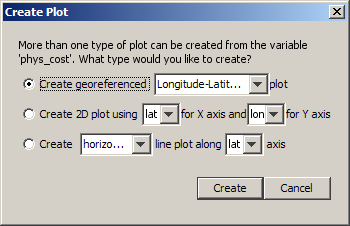
\includegraphics[scale=2.0]{CreatePlot.png}
\end{center}
\caption{\textbf{Panoply} \textsf{Create Plot} dialogue window.}
\label{fig:CreatePlot}
\end{figure}

You can interpolate the data or not (often you may find that it is clearer not to interpolate the data but to leave it as 'blocky' colors corresponding to the resolution of the model), change the scale and colors, overlay continental outline, change the projection, etc etc. Gray cells represent 'dry' grid points, i.e., continental or oceanic crust.
To save plots in \textbf{Panoply} -- from the file menu: \footnotesize\textsf{File}\normalsize, then \footnotesize\textsf{Save Image As ... }\normalsize and then select the location, filename, and graphics format.

%------------------------------------------------

\subsection{Issues with Panoply default settings}

The default settings in \textbf{Panoply}, i.e. those used when a plot is first created, can often mislead. In particular, note:
\begin{itemize}

\vspace{1mm}
\item \footnotesize\textsf{Year }\normalsize (\footnotesize\textsf{Array}\normalsize tab)
        \\ The default is for the very 1st \textit{time-slice} to be displayed rather than the experiment end. The first \textit{time-slice} is numbered from 1 to however many total time-slices have been saved (displayed to the immediate right of the \footnotesize\textsf{Year ,}\normalsize box), and it is this integer number that appears in the \footnotesize\textsf{Year }\normalsize box -- not the year of the data save. Instead, the mid-point year of the time-slice is displayed in a second box (labeled '\footnotesize\textsf{Year mid-point}\normalsize').
        \\ Different \textit{time-slices} to be plotted can be selected by either clicking through the saved year count, or by selecting the save year mid-point from the drop-down list.

\vspace{1mm}
\item \footnotesize\textsf{Scale Range }\normalsize (\footnotesize\textsf{Scale}\normalsize tab)
        \\ The color scale is auto-scaled so that the range always goes from the minimum to maximum displayed value. This can potentially mislead if save years and/or depth/latitude slices are scrolled through as the scale will be automatically adjusted to fit each plot in turn.
        \\ Confusion can also arise for fields with no variation, e.g. atmospheric trace gas concentrations or air temperature -- the auto-scaled plot in these instances has a uniform color but with odd hatching as Panoply dutifully tries to achieve the impossible (creating a scale of multiple colors for a single value).

\vspace{1mm}
\item Zonal averaging (\footnotesize\textsf{Array }\normalsize tab)
        \\ \footnotesize\textsf{Lat-Vert }\normalsize plots are displayed as a zonal mean by default. This is indicated by the tick in the \footnotesize\textsf{Ave }\normalsize box (bottom RH corner). Un-ticking the \footnotesize\textsf{Ave }\normalsize box releases the averaging with the first longitudinal value of the grid now displayed instead. Similar to how Panoply displays years -- the longitudinal grid locations are counter from 1 to typically 36 (depending on the resolution of the ocean grid), with the longitudinal mid-point value in degrees East displayed to the right.
        \\ Different longitudinal sections to be plotted can be selected by either clicking through the grid point number count, or by selecting the longitudinal mid-point from the drop-down list.

\vspace{1mm}
\item Scale bar tick marks (\footnotesize\textsf{Array }\normalsize tab)
        \\ The tick labels on the color scale are displayed by default in the format: \footnotesize\textsf{x.y }\normalsize. If the typical values of the variable are order e.g. 10\begin{math}^{-6}\end{math} you will end up with value labels ranging from \footnotesize\textsf{0.0 }\normalsize to \footnotesize\textsf{0.0 }\normalsize ... This can be most easily resolved in one of two ways:
        \begin{itemize}
\item The format of the label can be changed by selecting a different option from the pull-down \footnotesize\textsf{Tick Label Format }\normalsize box (default == \footnotesize\textsf{\%.1f}\normalsize). For instance, \footnotesize\textsf{\%.2e }\normalsize would give a display in the format \footnotesize\textsf{x.xxEyy }\normalsize (or \footnotesize\textsf{x.xxE-yy}\normalsize) or \footnotesize\textsf{\%.6f }\normalsize would give \footnotesize\textsf{x.xxxxxx}\normalsize.
\item An alternative is to re-scale the values. This is done in the Scaling Factor box in which you set the scale factor in powers of 10. For example: setting \footnotesize\textsf{-6}\normalsize in effect converts units of mol kg\begin{math}^{-6}\end{math} to \begin{math}\mu\end{math}mol kg\begin{math}^{-6}\end{math}.
\end{itemize}

\vspace{1mm}
\item Other things to watch out for include:
\begin{itemize}
\item A plot involving depth, being by default, 'up-side-down'!.
\\This is fixed in the \footnotesize\textsf{Grid}\normalsize tab, and the click button, \footnotesize\textsf{Swap B/T}\normalsize.
\item In \footnotesize\textsf{'Lon-Lat'}\normalsize plots, the modern continental outline being displayed by default.
\\This can be fixed by changing options in the \footnotesize\textsf{Overlay}\normalsize tab.
\end{itemize}

\end{itemize}
\vspace{2mm}

\begin{center}
\textbf{Simply be careful when opening a new plot that you are looking at what you *think* you are looking at (or what you think you are looking at *is* what you are looking at).}
\end{center}

Note that default plotting settings in \textbf{Panoply} can be changed (and saved).

%------------------------------------------------

\subsection{Basic plots -- examples}

\vspace{1mm}
\noindent\rule{4cm}{0.5pt}
\vspace{2mm}

\noindent\textcolor{red}{TO COME ...}

\vspace{1mm}
\noindent\rule{4cm}{0.5pt}
\vspace{2mm}

%------------------------------------------------

\subsection{Difference (anomaly) plots}

It is possible to create an anomaly (difference) maps in \textbf{Panoply} which are essential when analyzing changes in a variable that may be small compared to the global spatial variability. To do this:

\begin{itemize}
\vspace{1mm}
\item First, open the netCDF results file.
\vspace{1mm}
\item Open the variable of interest, e.g., \texttt{atm\_temp} (surface air temperature) in the 2D netCDF file.
\vspace{-4mm}
\item From the upper LH corner of the Dataset Browser window, from the drop-down menu, select the name of the plot you have just created (\texttt{atm\_temp} in \footnotesize\textsf{field\_biogem\_2D}\normalsize ...).
\vspace{1mm}
\item From the upper LH corner of the Dataset Browser window, now click on the \footnotesize\textsf{Combine Plot}\normalsize icon.
\\ You now have a plot window that is displaying a difference map. By default, it is showing you the difference between two identical (in time) slices. The two different slices are labeled Array 1 (LH side) and Array 2 (RH side).
\\NOTE: Easier than mucking about with \footnotesize\textsf{Combine Plot}\normalsize, is having open the first dataset, simply drag another variable from the list of variables in the \footnotesize\textsf{Sources }\normalsize window, into the \footnotesize\textsf{Plot }\normalsize window. You can drag either a different, or the same variable, into the \footnotesize\textsf{Plot }\normalsize window.
\end{itemize}
\vspace{2mm}

For instance, you can keep one array (Array 1) fixed to the initial (year 1 (centered on 0.5)) and vary the year in the second array (Array 2). Note that you can select in Panoply whether Array 1 - Array 2 is plotted, or Array 2 - Array 1, or various proportional or relative differences.

If you switch off the auto-scaling feature (\footnotesize\textsf{Always fit to data}\normalsize) you can center the scale so that no change is white, with positive deviations = red and negative = blue by clicking on Center on 0. This is something of a convention in the scientific literature.

The same variable in two different model experiments can also be opened up and analyzed combined:

\begin{itemize}
\vspace{1mm}
\item Start by opening up both required netCDF files.
\vspace{1mm}
\item Open the variable of interest in one (either one) of the two 2D netCDF data-sets.
\vspace{1mm}
\item From the upper LH corner of the Dataset Browser window, from the drop-down menu, select the name of the plot you have just created.
\vspace{1mm}
\item Now double-click in the variable in the 2nd netCDF dataset.
\\ You now have a plot window that is displaying a difference map, but of the same variable between two different experiments, rather than two years of the same experiment.
\end{itemize}
\vspace{2mm}

%------------------------------------------------

\subsection{Ocean velocity plots}

By combining the two (horizontal) fields of ocean circulation, rather than a difference plot, \textbf{Panoply} can create a velocity plot. This is a great way of visualizing surface (and deeper) currents and circulation patterns. To do this:

\begin{itemize}
\vspace{1mm}
\item First, open the 3-D netCDF results file.
\vspace{1mm}
\item Open either the \texttt{phys\_u} ('ocean velocity - u') or \texttt{phys\_v} ('ocean velocity - v') field and select a \footnotesize\textsf{Lon-Lat }\normalsize plot.
\vspace{1mm}
\item From the upper LH corner of the \footnotesize\textsf{Sources }\normalsize window, from the drop-down menu, select the name of the plot you have just created.
\vspace{1mm}
\item Now double-click on the other velocity variable (whichever of the u and v fields you did not open first).
\vspace{1mm}
\item By default you get a difference map, which is pretty useless really. From the drop-down \footnotesize\textsf{Plot }\normalsize menu box (which should be displaying 'Array 1 - Array 2' by default) select: \footnotesize\textsf{Vector Magnitude }\normalsize(bottom of the list).
\\ You now have a plot window that is displaying the ocean velocity field, with arrows indicating the direction and speed (length of the arrow) together with an interpolated color background of the speed.
\end{itemize}
\vspace{2mm}

You can re-scale the velocity arrows to more clearly display the circulation pattern by altering the \footnotesize\textsf{Scale Length }\normalsize value (\footnotesize\textsf{Contours \& Vectors }\normalsize tab). A value of 0.1 is a reasonable choice for surface currents. e.g. see Figure \ref{fig:cgenie_currents}.

If you want to display deeper (in the ocean) current fields and/or different time-slices, take care that the depth level (/time-slice) in both LH and RH sides of the \footnotesize\textsf{Array(s) }\normalsize panel must be changed to the same value. If displaying deeper current fields, then the velocity vectors will have to be further re-scaled (to a smaller value) in line with the lower velocities at depth compared to the surface.

\newpage

\begin{figure}[ht]
\begin{center}
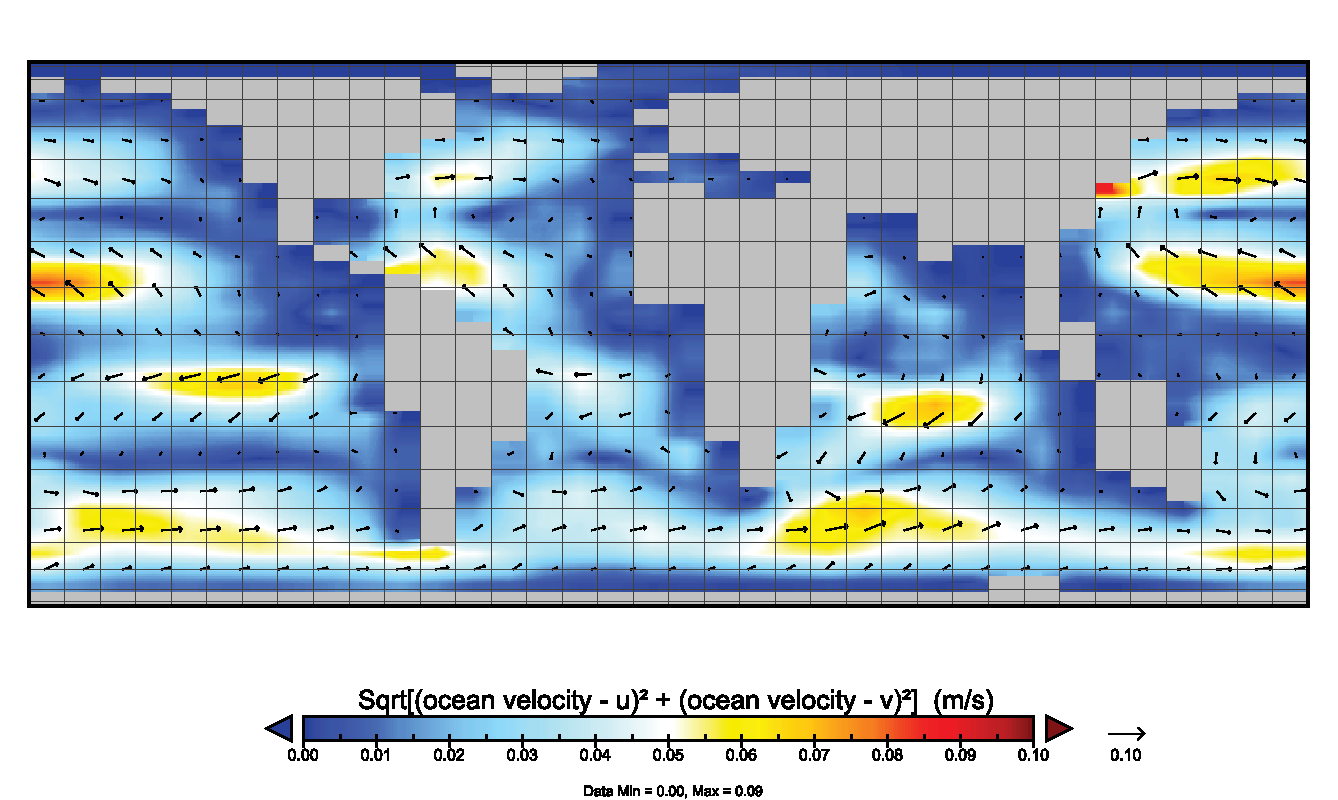
\includegraphics[scale=0.5]{cgenie_currents.pdf}
\end{center}
\caption{Example (modern) ocean surface velocity (current) map.}
\label{fig:cgenie_currents}
\end{figure}

%------------------------------------------------

\newpage

%------------------------------------------------

\section{MATLAB plotting}

%------------------------------------------------

\subsection{MATLAB 101}

If you need a tutorial on \textbf{MATLAB}, either as a refresher, or because you have not used the program before, refer to (and/or work through) the following sections of the \href{https://github.com/derpycode/matlabananas\#matlabananas}{matlabananas} \textbf{MATLAB} textbook:

\vspace{2pt}
\begin{itemize}
\vspace{1pt}
\item Chapter 1 --  this covers the very basics of using \textbf{MATLAB}, what variables are, including scalars (e.g. single numbers), vectors (1D array), matrices (2D array) and higher order arrays, now to index and carry out basic manipulation of arrays, basic data loading and saving and plotting.
\vspace{1pt}
\item Sections 2.1 and 2.2 of Chapter 2, which cover creating (script) programs -- i.e. adding all your \textbf{MATLAB} commands to a file (a \footnotesize\textsf{.m }\normalsize or '\footnotesize\textsf{m-file }\normalsize') and running the file, and \textit{functions} -- programs (\footnotesize\textsf{m-file}\normalsize s) where one or more parameters might be passed into the \textit{function} when it is called (e.g. at the command line), and potentially variables returned.
\vspace{1pt}
\item In Chapter 3 -- subsection 3.1.3 deals with reading in netCDF format data, which is the \textbf{muffin} format for spatial data. Section 3.2 deals with more advanced 2D plotting (also of direct relevance to \textbf{muffin} data processing and visualization using \textbf{MATLAB}).
\end{itemize}
\vspace{2pt}

%------------------------------------------------

\subsection{MATLAB and ASCII (\textit{time-series})}

The \textit{time-series} (\textsf{\footnotesize .res}) output of \textbf{BIOGEM} are in a simple plain text (ASCII) format. These can be read in very easily in \textbf{MATLAB} using the \texttt{load} command. Note that a brief description of each column of data in the \textit{time-series} files appears on the first first line of the file, and that prefixing this is a \texttt{\%} symbol, that \textbf{MATLAB} ignores. Hence only the columns of data gets read in by default using \texttt{load} :) \footnote{There are also other \textbf{MATLAB} commands for reading in text data -- refer to to the \href{http://www.seao2.info//teaching/201718.GEO111/GEO111.pdf}{\textbf{MATLAB} programming text}.} For example:

\small\begin{verbatim}
>> co2=load('biogem_series_atm_pCO_2.res','-ascii');
>> plot(co2(:,1),1.0E6*co2(:,3));
\end{verbatim}\normalsize

\noindent loads in the atmospheric \(CO_{2}\) time-series file (assigning it to the array variable \texttt{co2}), and then plots (as a line graph) the 3rd column (\(CO_{2}\) concentration) vs. the first (time). Because concentrations are saved in units of atmospheres, a factor of \texttt{1.0E6} is applied to concert to \(\mu atm\). Equivalently:

\small\begin{verbatim}
>> co2=load('biogem_series_atm_pCO2\).res','-ascii');
>> scatter(co2(:,1),1.0E6*co2(:,3));
\end{verbatim}\normalsize

%------------------------------------------------

\subsection{MATLAB 'Import Data' ...}

You can also import the time-series files by clicking on the \footnotesize\textsf{Import Data }\normalsize icon:

\begin{itemize}
\vspace{1pt}
\item Navigate to the \textbf{BIOGEM} sub-directory of your experiment results directory. Ensure that \footnotesize\textsf{All Files }\normalsize is selected and click on the time-series file you want.
\vspace{1pt}
\item \textbf{MATLAB} ignores the header lines, and it should be safe to simply click on \footnotesize\textsf{Import Selecftion }\normalsize for all columns, or select what you want to plot -- typically year (the first column) and another one.
\vspace{1pt}
\item A default variable name -- the filename minus the underscore characters -- will appear listed in the \textbf{MATLAB} \footnotesize\textsf{Workspace window }\normalsize. Double-click on the variable name to open up the imported data in a table view. If you select columns to plot, and then head over to the main \footnotesize\textsf{PLOTS }\normalsize tab, a range of plotting options are provided and a plot can be generated by clicking on one of the plotting icons.\footnote{Note that if you have not selected any data columns, then all the plotting icons are disabled and greyed out in the \footnotesize\textsf{PLOTS }\normalsize tab.}
\vspace{1pt}
\item Labels can be added, scales and markers changed, etc etc, in the \footnotesize\textsf{Figure window }\normalsize.
\end{itemize}
\vspace{2pt}

Note that as the data has been imported as an array in \textbf{MATLAB}, you can also plot directly from the command line. (And indeed, you could also have loaded the data from the command line.)

%------------------------------------------------

\subsection{MATLAB and netCDF (\textit{time-slice})}

\noindent Basically -- the only hard part, having opened the \textit{netCDF} file is in correctly deducing which dimension in an extracted data array is   longitude, latitude, (sometimes depth), or time. Mostly this should be pretty obvious from inspecting the \textbf{MATLAB} \footnotesize\textsf{Workspace }\normalsize window (assuming you have a column for \footnotesize\textsf{Size }\normalsize selected to be displayed), or using the \texttt{size} command.\footnote{It also turns out that the order of dimensions for a variable read in by \textbf{MATLAB}, is the opposite of the order listed in the \textsf{Variable} window of \textbf{Panoply}.} Once you have done this, you can plot slices, scale data, average or otherwise process data, extract locations at specific locations, etc etc.

As an example -- in \textbf{MATLAB}, first either change directory to the \textsf{\small biogem} directory of a set of \textbf{muffin} results, or from where-ever you are, add a path to the location of the \textsf{\small biogem} directory. To open the 2D \textbf{BIOGEM} netCDF results file, type:
\begin{verbatim}
>> ncid = netcdf.open('fields_biogem_2d.nc','nowrite');
\end{verbatim}

To extract a variable, you first need to find its ID from its name:
\begin{verbatim}
>> varid = netcdf.inqVarID(ncid,NAME);
\end{verbatim}
where \texttt{NAME} is a place-holder for the name of he variable (as a string). You might need to use \textbf{Panoply} to display all the different variable names. Or, you can list all the variables and stuff in the netCDF file using \texttt{ncdisp}:
\begin{verbatim}
>> ncdisp('fields_biogem_2d.nc')
\end{verbatim}

Having, by one means or another, identified the name of the variable you are interested in, you can recover its ID and then the data itself, for example, for \textsf{\footnotesize atm\_temp} (\textsf{\footnotesize surface air temperature}):
\begin{verbatim}
>> varid = netcdf.inqVarID(ncid,'atm_temp');
>> data  = netcdf.getVar(ncid,varid);
\end{verbatim}

In loading in the variable, you end up with a multi-dimensional array -- 2 spatial dimensions and if you have more than 1 \textit{time-slice} of data saved, 1 temporal dimension (and if you loaded in the \textbf{BIOGEM} 3D netCDF file, you end up with a 4-dimensional array). \textbf{MATLAB} reports the size of the array in the \textsf{\footnotesize Workspace window} (depending on which column display options you have selected). In the example here, which took the experiment \textsf{\footnotesize EXAMPLE.worjh2.Caoetal2009.RCP6p0}, the array for atmospheric temperature is reported as \(36\times36\times8\).\footnote{Although note that in \textbf{Panoply}, it is reported as \textsf{\scriptsize atm\_temp(time=8, lat=36, lon=36)}.} so the last of the 8 time-slices would  be accessed as:
\begin{verbatim}
>> data_last = data(:,:,8);
\end{verbatim}
or
\begin{verbatim}
>> data_last = data(:,:,end);
\end{verbatim}

Panoply reports variables in the the \textbf{BIOGEM} 3D netCDF file as having dimensions of: (\textit{time, zt, lat, lon}) (e.g. (time=13, zt=16, lat=36, lon=36)) whereas \textbf{MATLAB} reads it in the reverse order. For instance, if we load in the (3D) ocean temperature field:
\begin{verbatim}
>> ncid = netcdf.open('fields_biogem_3d.nc','nowrite')
>> varid = netcdf.inqVarID(ncid,'ocn_temp');
>> data  = netcdf.getVar(ncid,varid);
\end{verbatim}
and then type:
\begin{verbatim}
>> size(data)
ans =
    36    36    16    13
\end{verbatim}
we get an array orientated as (\textit{lon, lat, zt, time}).\footnote{\textit{zt} is the depth level in the ocean.} The final time-slice would hence then be accessed:
\begin{verbatim}
>> data_last = data(:,:,:,end);
\end{verbatim}
with \texttt{data\_last} now becoming a 3D array with dimensions (\textit{lon, lat, zt}).

\vspace{2mm}
There are three key things to remember at this point:

\begin{enumerate}
\setlength{\itemindent}{.2in}

\vspace{1mm}
\item Firstly, the depth levels are read such that index \texttt{1} is the surface, and \texttt{16} is the deepest ocean depth level (in this case, otherwise it is \texttt{8}).

\vspace{1mm}
\item For the lon-lat part -- (\textit{lon, lat}) equates to \textit{row}\textit{}s vs. \textit{columns} in \textbf{MATLAB}, and hence if you were to plot e.g. the surface ocean slice:
\begin{verbatim}
>> imagesc(data_last(:,:,1));
\end{verbatim}
you will end up with the plot on its side, with latitude along the \textit{x}-axis and longitude on the \textit{y}-axis.
\\You can exchange rows and columns in \textbf{MATLAB} with the \textit{transpose operator} (see programming/\textbf{MATLAB} book):
\begin{verbatim}
>> imagesc(data_last(:,:,1)');
\end{verbatim}
but ... this still leaves you with an up-side-down plot, because \textbf{MATLAB} reads from the first row down, whereas in latitude, you are expecting to read from -90 degrees up (towards the N pole). \texttt{flipud} accomplishes the final transformation:
\begin{verbatim}
>> imagesc(flipud(data_last(:,:,1)'));
\end{verbatim}

\vspace{1mm}
\item The final complication is that \textbf{muffin} netCDF output uses a special value to represent an invalid or null number, e.g. for ocean temperature where the grid point is land (and an ocean temperature value would have no meaning). In the netCDF definition, \textbf{Panoply} is told what the special number is, hence it shows land in grey when plotting ocean variables.

Panoply reports this as: \textsf{\footnotesize missing\_value = 9.969209968386869E36}.

\vspace{1mm}
There is no easy way (that I can see!) to get \textbf{MATLAB} to deal with this for you, so you need to search and replace this value, e.g.:
\small\begin{verbatim}
>> null=9.969209968386869E36;
>> data_last(find(data_last==null))=NaN;
\end{verbatim}\normalsize
which searches for this null value and replaces it with a \texttt{NaN} (so that now it can be simply plotted).

\end{enumerate}
\vspace{2mm}

Once you are done accessing data, it is good practice to close the netCDF file after you are done with it:
\begin{verbatim}
>> netcdf.close(ncid);
\end{verbatim}

The question then remains: what do you actually 'do' with it in \textbf{MATLAB}?

%------------------------------------------------

\subsubsection{Plotting sections}

For a quick look-see, \texttt{imagesc} (as per above) is handy.

\noindent For more advanced plotting (and for presentation) -- refer to the \textbf{matlabananas} \textbf{MATLAB} programming text.

\noindent As per above, horizontal (lon-lat) fields can be extracted from 2D \textit{netCDF} output by: \texttt{data(:,:,time)} and from 3D by: \texttt{data(:,:,zt,time)}. Obviously, you could also extract lon-depth via: \texttt{data(:,lat,:,time)} and lat-depth via: \texttt{data(lon,:,:,time)}.

\noindent Anomalies (with time) are created: \texttt{data(:,:,:,time2)-data(:,:,:,time2)}.

Typically, except a little trial-and-error in extracting the dimensions you want, and also in correcting the orientation of the matrix or resulting plot.

%------------------------------------------------

\subsubsection{Calculating inventories}

Often, the inventory (total mass or number of moles) of the ocean or atmosphere is useful to know, particularly as a function of time. For the ocean (or atmosphere) as a whole, the \textit{time-series} output files report this (alongside the mean global concentration).

You can also calculate this with \textbf{MATLAB} from the netCDF output. Fields of ocean concentration are saved in the 3D output (and atmospheric concentrations in the 2D output). To convert concentration in the ocean, in units of \(molkg^{-1}\) you'll need to know the mass of each ocean cell, in units of \(kg\).

When saving using save option \texttt{9}, or \texttt{99}\footnote{Parameter \texttt{bg\_par\_data\_save\_level} -- see earlier.}, you save the 'physics' of the ocean model, which is actually mostly just the grid information, such as cell area, thickness, latitude and longitude edges and midpoints, depth edges and mid point. Also saved are the masses and volumes of the grid of cells. So to derive an array of cell tracer inventories from an array of concentrations, and the array of cell masses (variable \textsf{\footnotesize phys\_ocn\_M}), you'd write:

\pagebreak

\small\begin{verbatim}
varid = netcdf.inqVarID(ncid,'ocn_temp');
data  = netcdf.getVar(ncid,varid);
varid = netcdf.inqVarID(ncid,'phys_ocn_M');
mass  = netcdf.getVar(ncid,varid);
inventory = data(:,:,:,time).*mass(:,:,:,time);
\end{verbatim}\normalsize
\noindent Before summing \texttt{inventory} to determine the global total inventory, you will, as before, have to deal with the null values (converting them to \texttt{NaN}) and then deal with the presence of \texttt{NaN}s in the array when summing ...

The advantage of doing the calculations in \textbf{MATLAB} (despite being provided with the global mean and inventory in the time-series files) is that you could calculate the inventory of a tracer (/substance) for just the ocean surface, or just a specific region of band of latitude. Or you could calculate the mean concentration for just a specific region of the ocean.\footnote{In calculating mean concentrations, you'll need to volume or mass weight the concentrations, and hence still need to use one of the physics variables.}

%----------------------------------------------------------------------------------------
%----------------------------------------------------------------------------------------
%%----------------------------------------------------------------------------------------
%       CHAPTER 15
%----------------------------------------------------------------------------------------

\cleardoublepage

\chapterimage{chx-plotting.png} % Chapter heading image

\chapter{muffinplot}\label{ch:muffinplot}

\hfill \break

%------------------------------------------------
\newpage
%------------------------------------------------

\section{(none)}

%----------------------------------------------------------------------------------------
%----------------------------------------------------------------------------------------
%----------------------------------------------------------------------------------------
%       CHAPTER 16
%----------------------------------------------------------------------------------------

\cleardoublepage

\chapterimage{chx-plotting.png} % Chapter heading image

\chapter{muffinplot}\label{ch:muffinplot}

\hfill \break

%------------------------------------------------
\newpage
%------------------------------------------------

\noindent The \textbf{muffinplot} suite of \textbf{MATLAB} functions provides a means of plotting a variety of output reproducibly (by means of  a saved parameter file) and with the potential for automation (i.e. automatically generating the same analysis for a large number of different experiments).

The functions comprising this software suite include:

\begin{itemize}[noitemsep]
\vspace{1mm}
\item \footnotesize\textsf{plot\_fields\_biogem\_2d}\normalsize -- lon-lat plots from the 2D \textbf{biogem} output.
\vspace{1mm}
\item \footnotesize\textsf{plot\_fields\_biogem\_3d\_i}\normalsize -- lat-depth plots from the 3D \textbf{biogem} output.
\vspace{1mm}
\item \footnotesize\textsf{plot\_fields\_biogem\_3d\_k}\normalsize -- lon-lat plots from the 3D \textbf{biogem} output.
\vspace{1mm}
\item \footnotesize\textsf{plot\_fields\_ccd}\normalsize -- analsysis of the 'CCD' (from both \textbf{biogem} 2D and \textbf{sedgem} 2D output).
\vspace{1mm}
\item \footnotesize\textsf{plot\_fields\_sedgem\_2d}\normalsize -- lon-lat plots from the 2D \textbf{sedgem} output.
\vspace{1mm}
\item \footnotesize\textsf{plot\_histc\_2d}\normalsize -- a generic color-coded histogram function.
\vspace{1mm}
\item \footnotesize\textsf{plot\_sedcore}\normalsize -- down-core plots from \textbf{sedgem} sedcore output.
\vspace{1mm}
\item \footnotesize\textsf{plot\_timeseries\_biogem}\normalsize -- time-series plots from \textbf{biogem} time-series output.
\end{itemize}
Note that at this current time, there is no facility for lon-depth plotting (unlike in \textbf{Panoply}).

Most of the plots also perform additional functions (which can be generally disabled if not wanted), such as plotting and saving zonal or depth profiles, plotting difference maps, plotting and labelling data on maps and carrying out model-data fit statistics and plotting, extracting model values at data locations.

The following sections provide an overview and examples of such plotting and analysis.

%------------------------------------------------

\section{Installation}

\textbf{muffinplot} can be obtained from \href{https://github.com/derpycode/muffinplot\#https://github.com/derpycode/muffinplot}{github}. If you do not have a \textbf{git} client on your computer (and hence cannot clone the repository locally), then simply download the archive file of all the code (from \footnotesize\textsf{\textcolor[rgb]{0,0.501961,0}{clone or download }}\normalsize -- pick \textsf{\footnotesize Download ZIP}).

When you unpack (or clone) \textbf{muffinplot} (note that it is likely to unpack by default into its own directory), you should see 3 directories -- \footnotesize\textsf{EXAMPLES}\normalsize, and \footnotesize\textsf{MASKS}\normalsize,\ \footnotesize\textsf{source}\normalsize, a series of \footnotesize\textsf{.m }\normalsize files, and a single lonely \footnotesize\textsf{.ps }\normalsize graphics file (\footnotesize\textsf{colorscales.ps}\normalsize). The \footnotesize\textsf{.m }\normalsize files are split into filenames with or without the label \footnotesize\textsf{SETTINGS }\normalsize -- the ones without are code files (\textit{functions}), and the ones with the word \footnotesize\textsf{SETTINGS }\normalsize in their filename, contain parameter settings for plotting.

By default (the parameters can be changed if you wish), wherever you run the \textbf{muffinplot} plotting function from, requires that you also have a subdirectory called \footnotesize\textsf{cgenie\_output}\normalsize\ present, and that the (complete) \textbf{muffin} experiment output directories of anything you want to plot should be in subdirectories of that -- i.e. the contents of \footnotesize\textsf{cgenie\_output }\normalsize should look like the contents of \footnotesize\textsf{cgenie\_output }\normalsize on your cluster account\footnote{Although you do not need to copy \uline{all} the results over ... just the experiments that you wish to plot up.}. Mask files reside in the \footnotesize\textsf{MASKS}\normalsize\ subdirectory of the \textbf{muffinplot} installation, or in your current directory, or anywhere in the \textbf{MATLAB} path.

The simplest option is to unpack/clone \textbf{muffinplot} to a directory containing \footnotesize\textsf{cgenie\_output }\normalsize and hence all your experimental results directories.\footnote{However, the \textbf{muffinplot} functions do not have to be run from the same directory that you are in -- you can install them somewhere convenient, and then with \textbf{MATLAB} set to a directory containing a \textsf{cgenie\_output} experiment results directory, you can:
\\\texttt{>> addpath(PATH)}
\\where \texttt{PATH} is the path to the directory where \textbf{muffinplot} is installed.}
In other words:
\begin{enumerate}[noitemsep]
\vspace{1mm}
\item Create some local directory e.g. called \footnotesize\textsf{RESULTS}\normalsize.
\vspace{1mm}
\item Create a subdirectory in \footnotesize\textsf{RESULTS }\normalsize called \footnotesize\textsf{cgenie\_output}\normalsize.
\vspace{1mm}
\item Drag your experiment results folders across into the subdirectory \footnotesize\textsf{cgenie\_output}\normalsize, as per the directory structure on the cluster. (Or better -- drag the archived files to  \footnotesize\textsf{cgenie\_output }\normalsize and unpack them.)
\vspace{1mm}
\item Install \textbf{muffinplot} in the \footnotesize\textsf{RESULTS }\normalsize directory.
\vspace{1mm}
\item Change the \textbf{MATLAB} working directory to \footnotesize\textsf{RESULTS}\normalsize.
\end{enumerate}
\vspace{2mm}

The plotting functions are run simply by typing their name and passing a list of parameters (comma-separated, with the complete list enclosed in parentheses). By default,   the \footnotesize\textsf{SETTINGS }\normalsize files need to be in the same directory as you are running the functions from, or in one of the \textbf{MATLAB} paths. Results are saved to a subdirectory that by default is called \footnotesize\textsf{PLOTS}\normalsize, which will be created for you if it does not already exist.

All the plotting functions provide some manner of 'help', that can be obtained by typing at the command line:
\vspace{-2pt}\begin{verbatim}
>> help FUNCTIONNAME
\end{verbatim}\vspace{-2pt}
where \texttt{FUNCTIONNAME} is the function name (as per listed above).

%------------------------------------------------

\newpage 
\section{Time-series plotting}

The \textbf{muffinplot} function \textsf{\footnotesize plot\_timeseries\_biogem.m} provides a facility to plot \textbf{BIOGEM} \textit{time-series} (\textsf{\small .res}) output.\footnote{Obviously -- there are lots of different and easy ways of plotting plain text output in the form of a simple column format.} You can use \textbf{MATLAB} \texttt{help} on the function name to detail the parameters that need to be passed (and examples).

The \textsf{\footnotesize plot\_timeseries\_biogem} plotting function plots a basic set of time-series variables by default. It then, enables a set up up to 3 additional variables to be plotted. It is also associated with a file of parameter values (\textsf{\footnotesize plot\_timeseries\_SETTINGS.m} by default) for fine-tuning plots.

The plotting function requires a list of parameters to be passed in the argument list, i.e.:
\begin{verbatim}
>> plot_timeseries_biogem(PAR1,PAR2,PAR3, ... PARn)
\end{verbatim}

These are, in order:

\vspace{1mm}
\begin{enumerate}
\item \texttt{PEXP1} -- \textit{string} \(\rightarrow\) the (first) experiment name.
\item \texttt{PEXP2} -- \textit{string} \(\rightarrow\)  is the name of the 2nd (optional) experiment. If no second experiment is selected, then a null string value must be passed, i.e., \texttt{''}.
\item \texttt{PTMIN} -- \textit{real} \(\rightarrow\) minimum plotted time (\textit{x}-axis).
\item \texttt{PTMAX} -- \textit{real} \(\rightarrow\) maximum plotted time (\textit{x}-axis).
\item \texttt{PDATA1} -- \textit{string} \(\rightarrow\) time-series variable name for additional data to plot.
\\Omit the '\texttt{biogem\_series\_}' and '\texttt{.res}' parts of the filename.
\\Leave blank, i.e., '', for no additional data panel.
\item \texttt{PDATA1N} -- \textit{integer} \(\rightarrow\) the column number of the data in the time-series file.
\item \texttt{PDATA2} -- \textit{string} \(\rightarrow\) time-series variable name for additional data to plot.
\item \texttt{PDATA2N} -- \textit{integer} \(\rightarrow\) the column number of the data in the time-series file.
\item \texttt{PDATA3} -- \textit{string} \(\rightarrow\) time-series variable name for additional data to plot.
\item \texttt{PDATA3N} -- \textit{integer} \(\rightarrow\) the column number of the data in the time-series file.
\item \texttt{POPT} -- \textit{string}\(\rightarrow\) The string for an alternative plotting parameter set.
\\If an empty\texttt{ ('') }value is passed as this parameter, then the default parameter set file is used.
\item \texttt{PNAME}  -- \textit{string}\(\rightarrow\) The string for an alternative filename.
\end{enumerate}
\vspace{2mm}
Note that if an empty value is passed as this parameter, then a filename is automatically generated.

A simple example usage would be:

\begin{verbatim}
>> plot_timeseries_biogem('myexperiment','',0.0,10000.0,'',0,'',0,'',0,'','')
\end{verbatim}
where \texttt{myexperiment} is the name of the 1st experiment, followed by and empty string (\texttt{''}) indicating no second experiment. The results are to be plotted from 0.0 to 10000.0 years (the 2 following parameters; \texttt{0.0,10000.0}). Then, no additional (maximum 3) optional parameters are requested, and hence the next parameters passed are: \texttt{'',0,'',0,'',0}. Finally, the default plotting parameter set is required, and no specific alternative filename is ot be used, accounting for the final 2 empty strings passed.

By default, \textsf{\footnotesize plot\_timeseries\_biogem} plots 2 panels of data, both with 2 (LH\ and RH) axes:

\begin{enumerate}[noitemsep]
\vspace{1mm}
\item Atmospheric \(CO_{2}\). Note that if the experiment was not \(CO_{2}\)-enabled (i.e. not run with a global carbon cycle), a warning is given and 'fake' data (actually, random numbers) is plotted.
\vspace{1mm}
\item Atmospheric \(\delta ^{13}CO_{2}\). Note that if the experiment was not \(\delta ^{13}CO_{2}\)-enabled (i.e. not run with a global carbon cycle), a warning is given and 'fake' data is plotted.
\vspace{1mm}
\item Atmospheric temperature (as a global mean, annual average).
\vspace{1mm}
\item Fractional (percentage) sea-ice extent.
\end{enumerate}
\vspace{2mm}

Additional model outputs can then be added by listing them in the function call. For example, to also plot the global overturning strength, which is contained in the file \footnotesize\textsf{biogem\_series\_misc\_opsi.res}\normalsize, you would add \texttt{'misc\_opsi',3}\footnote{Don't forget that you omit the '\texttt{biogem\_series\_}' and '\texttt{.res}' parts of the filename.}, where the \texttt{3} indicates the 3rd column of data in the file is to be plotted, which in this case is the global maximum overturning value (and the 2nd column is the minimum value). The complete line looks like:
\small\begin{verbatim}
>> plot_timeseries_biogem('myexperiment','',0.0,10000.0,'misc_opsi',3,'',0,'',0,'','')
\end{verbatim}\normalsize

By default, the plotted variables are all auto-scaled. To specify the y-axes, you will need to edit the plotting settings parameter file: \footnotesize\textsf{plot\_timeseries\_SETTINGS.m}\normalsize. For the default plotted 4 results variables, the minimum and maximum y-axis limits are specified in the section:
\vspace{1mm}
\begin{itemize}
\item[] \texttt{axis\_pCO2min = 0.0;}
\item[] \texttt{axis\_pCO2max = 0.0;}
\item[] \texttt{axis\_d13Cmin = 0.0;}
\item[] \texttt{axis\_d13Cmin = 0.0;}
\item[] \texttt{axis\_Tatmmin = 0.0;}
\item[] \texttt{axis\_Tatmmin = 0.0;}
\item[] \texttt{axis\_icemin = 0.0;}
\item[] \texttt{axis\_icemin = 0.0;}
\end{itemize}
\vspace{2mm}
The default zero values here, tell the plotting function to create an auto-scale for the y-axis.\footnote{Note the units of atmospheric \(CO_{2}\) as \(\mu atm\).} Following this in the parameter file, are the settings for the optional variable plotting:
\vspace{1mm}
\begin{itemize}
\item[] \texttt{axis\_data1\_min = 0.0;}
\item[] \texttt{axis\_data1\_max = 0.0;}
\item[] \texttt{axis\_data2\_min = 0.0;}
\item[] \texttt{axis\_data2\_max = 0.0;}
\item[] \texttt{axis\_data2\_min = 0.0;}
\item[] \texttt{axis\_data2\_max = 0.0;}
\end{itemize}
\vspace{2mm}

Note that if you want instead to copy and rename and then edit this settings file, you will need to pass the new (non-default) filename when calling the plotting function. For example, if you created a new parameter settings file: \footnotesize\textsf{settings\_NEW.m }\normalsize, then the \textit{function} call would look like:
\small\begin{verbatim}
>> plot_timeseries_biogem('myexperiment','',0.0,10000.0,'',0,'',0,'',0,'settings_NEW','')
\end{verbatim}\normalsize

%------------------------------------------------

\section{Spatial plotting}

%------------------------------------------------

\subsubsection{Overview}

4 of the \textbf{muffinplot} plotting functions provide spatial (2D) plotting capabilities:
\vspace{2mm}
\begin{itemize}

\item \texttt{plot\_fields\_biogem\_2d}
\\Plot a 2-D field from: \footnotesize\textsf{fields\_biogem\_2d.nc}\normalsize.

\item \texttt{plot\_fields\_biogem\_3d\_i}
\\Plot a vertical-meridional (2-D) slice through the ocean (i.e., all cells have the same \texttt{i} (longitudinal) coordinate value) from: \footnotesize\textsf{fields\_biogem\_3d.nc}\normalsize.
\\Options are  provided for averaging longitudinally over a supplied mask, which may be the entire ocean and hence giving a global meridional cross-sectional mean, of a specific ocean basin, or may be a single cell 'wide' longitudinally and take a meandering path hence simulating an ocean transect. An option is also provided to overlay an ocean circulation stream-function.

\item \texttt{plot\_fields\_biogem\_3d\_k.m}
\\Plot a horizontal slice through the ocean from: \footnotesize\textsf{fields\_biogem\_3d.nc}\normalsize.
\\An option is provided for overlaying ocean circulation (velocity fields). Water column integrals  can also be calculated and displayed, as well as benthic surfaces, and the function can also determine the spatial distribution of the maximum or minimum value occurring anywhere in the water column (or portion of the water column).

\item \texttt{plot\_fields\_sedgem\_2d}
\\Plot a 2-D field from: \texttt{fields\_sedgem\_2d.nc}.

\end{itemize}
\vspace{2mm}

All 4 plotting functions can also overlay observed data and create difference (anomaly) maps -- either between different experiments, time-slices, or variables, or between model and data and provide summary statistics regarding the difference.

\subsubsection{Argument (parameter) list}

All 4 plotting functions share exactly the same format of parameters\footnote{Parameters can be in for form of strings, in which case they must be given as a series of characters enclosed in inverted commas \texttt{''}; as real numbers, e.g. \texttt{999.5} or \texttt{9.995E2}; or integers, e.g. \texttt{2}, \texttt{10}.} passed in the argument list:

\vspace{-2mm}
\small\begin{verbatim}
>> FUNCTIONNAME(PAR1,PAR2,PAR3, ... PARn)
\end{verbatim}\normalsize
\vspace{-2mm}
\noindent i.e. take a (long!) list of parameters. These are (in order):

\vspace{1mm}
\noindent Firstly, a series of parameters for defining experiment, variable, and year:

\vspace{1mm}
\begin{enumerate}
\item \texttt{PEXP1} -- \textit{string} -- is the name of the 1st (main) experiment. A results directory with the same name must exist in the directory \footnotesize\textsf{cgenie\_output}\normalsize\footnote{Or alternative directory if the default file path settings have been changed.}.
\item \texttt{PEXP2} -- \textit{string} -- is the name of the 2nd (optional) experiment. If no second experiment is selected, then a null string value must be passed, i.e., \texttt{''}.
\item \texttt{PVAR1} -- \textit{string} -- is the name of the 1st (main) variable. If no valid variable value is given, a list of valid variable names will be printed out.\footnote{As a string, the value must be encased in inverted commas: \texttt{''}.}
\item \texttt{PVAR2} -- \textit{string} -- is the name of the 2nd (optional) variable. If no second variable is selected, then a null string value must be passed, i.e., \texttt{''}.
\item \texttt{PT1} -- \textit{real} (or \textit{integer}) -- is the value of the 1st (main) time-slice. If no valid variable value is given, a list of valid variable names will be printed out.\footnote{As \textbf{sedgem} does not save multiple and/or time-specific data, a dummy value (anything) is entered here.}
\item \texttt{PT2} -- \textit{real} (or \textit{integer}) -- is the value of the 2nd (optional) time-slice. If no second time-slice is selected, then enter \texttt{-1}.\footnote{As \textbf{sedgem} does not save multiple and/or time-specific data, a dummy value (anything) is entered here.}
\end{enumerate}
\vspace{1mm}

Then there are 2 parameters for plotting sub-sets of the 2D or 3D data (essential for 3D data which cannot be usefully visualized in raw form):

\vspace{1mm}
\begin{enumerate}
\item \texttt{PIK} -- \textit{integer} -- varies in its interpretation and is discussed below.
\item \texttt{PMASK} -- \textit{string} -- is the name of an optional (2D) mask. A null string (\texttt{''}) must be passed if no mask is requested. A file with the same name (plus an extension \footnotesize\textsf{.dat}\normalsize) must exist in the directory \footnotesize\textsf{MASKS}\normalsize\footnote{Or alternative directory if the default file path settings have been changed.}. The interpretation of this parameter differs slightly between functions (below).
\end{enumerate}
\vspace{1mm}

Next come options for plotting scale control:

\vspace{1mm}
\begin{enumerate}
\item \texttt{PCSCALE} -- \textit{real} (or \textit{integer}) -- is the scale factor for the plot. For example, to plot in micro molar (umol kg-1) units, enter; \texttt{1e-6}. The plot is auto-scaled if a value of zero (\texttt{0.0}) is entered.
\item \texttt{PCMIN} -- \textit{real} (or \textit{integer}) -- is the minimum scale value.
\item \texttt{PCMAX} -- \textit{real} (or \textit{integer}) -- is the maximum scale value.
\item \texttt{PCN} -- \textit{integer} -- is the number of (contour) intervals between minimum and maximum scale values.
\end{enumerate}
\vspace{1mm}

Finally, there are 3 parameters for: specifying discrete (observed) data to be plotted (and analyzed against model projections), for specifying the plotting parameter file to be used, and for substituting an alternative filename for all the output:

\vspace{1mm}
\begin{enumerate}
\item \texttt{PDATA} -- \textit{string} -- is the filename containing the an overlay data set, which must be formatted as separated columns. The precise number and type of columns varies between different functions and also the plotting options chosen, and are hence discussed later. The full filename of this file must be give, \uline{including} any extensions (e.g. \footnotesize\textsf{.dat }\normalsize, \footnotesize\textsf{.txt}\normalsize). This parameter must be passed as a \textit{string}; leave blank, i.e., \texttt{''}, for no overlay data.
\item \texttt{POPT} -- \textit{string} -- is the \footnotesize\textsf{m-file }\normalsize filename (excluding the \footnotesize\textsf{.m }\normalsize extension) containing the plotting options (\footnotesize\textsf{SETTINGS}\normalsize). This parameter must be passed as a string; leave blank, i.e., \texttt{''}, in order to load the default file (\footnotesize\textsf{plot\_fields\_SETTINGS}\normalsize).
\item \texttt{PNAME} -- \textit{string} -- is the string for an alternative series of output filenames. This parameter must be passed as a string, e.g., \texttt{'experiment2'}. If an empty (i.e., \texttt{''}) value is passed to this parameter then the output filenames will be automatically generated.
\end{enumerate}
\vspace{1mm}

\vspace{1mm}
The basic parameter list for all 4 plotting functions\footnote{Note that for \texttt{plot\_fields\_sedgem\_2d} several of the parameters are redundant but \uline{must} still be included (typically as zeros). This is in order to retain a common parameter list format between all the different plotting functions.} is hence:
\footnotesize
\vspace{-4pt}\begin{verbatim}
>> FUNCTIONNAME(PEXP1,PEXP2,PVAR1,PVAR2,PT1,PT2,PIK,PMASK,PCSCALE,PCMIN,PCMAX,PCN,PDATA,POPT,PNAME);
\end{verbatim}\vspace{-4pt}
\normalsize

\subsubsection{Function specific interpretation of PIK and PMASK}

A note on the different behaviour of 2 of the passed parameters, depending on whcih plotting function is used -- \texttt{PIK}, and to some extent, \texttt{PMASK}, have quite different interpretations depending on the particular plotting function used:

\begin{enumerate}

\vspace{2pt}
\item \texttt{plot\_fields\_biogem\_2d}
\begin{enumerate}
\vspace{1pt}
\item \texttt{PIK} -- is the maximum depth (\texttt{k}) level that will be plotted, i.e. all depth levels deeper than \texttt{PIK} will be excluded. This is useful for plotting a variable only for the 'deep' ocean (rather than the ocean overlaying all ocean depths) for example. This value also provides an alternative way of creating a mask, and only values of \texttt{k} less than of equal to the passed value will be plotted.
\vspace{1pt}
\item \texttt{PMASK} -- is the name of an optional (2D) mask. A null string (\texttt{''}) must be passed if no mask is requested. (Shallow depths could also be excluded from the plot by means of a mask rather than setting \texttt{PIK}.)
\end{enumerate}

\vspace{2pt}
\item \texttt{plot\_fields\_biogem\_3d\_k}
\begin{enumerate}
\vspace{1pt}
\item \texttt{PIK} -- the depth (\texttt{k}) level to be plotted. Note that the levels are numbered from a maximum value designating the surface, to 1 for the deepest ocean level. Typically, maximum values for the number of ocean levels are \texttt{8} (e.g. \textit{Ridgwell et al.} [2007]) or \texttt{16} (e.g. \textit{Cao et al.} [2009]).
\\Non ocean level \texttt{k} values have special meanings here:
\begin{enumerate}[noitemsep]
\vspace{1pt}
\item \texttt{0}
\\A zero will result in a water column integral being plotted. With data, the model-data is  carried out on the grid as a whole.
\vspace{1pt}
\item \texttt{-1}
\\Will result in the benthic surface being plotted.
\end{enumerate}
\vspace{1pt}
\item \texttt{MASK} -- is the name of an optional (2D) mask. A null string (\texttt{''}) must be passed if no mask is requested.
\end{enumerate}

\vspace{2pt}
\item \texttt{plot\_fields\_biogem\_3d\_i}
\begin{enumerate}
\vspace{1pt}
\item \texttt{PIK} -- the longitude-depth (\texttt{i}) slice through the ocean to be plotted.
\\Non longitude grid point \texttt{i} values have special meanings here:
\begin{enumerate}[noitemsep]
\vspace{1pt}
\item \texttt{0}
\\A zero will result in a zonal mean being plotted. With data, model-data comparison is conducted at the specific data locations, rather than vs. a zonal mean model value.
\vspace{1pt}
\item \texttt{-1}
\\I have forgotten what this does ...
\end{enumerate}
\vspace{1pt}
\item \texttt{MASK} -- is the name of an optional (2D) mask. A null string (\texttt{''}) must be passed if no mask is requested.
\\ For example: if the mask is of the entire ocean (\texttt{mask\_worbe2\_ALL.dat}), the result is a global meridional cross-sectional mean.
\\ If the mask is just of a single basin such as the Atlantic (\texttt{mask\_worjh2\_Atlantic.dat}), the result is the Atlantic meridional cross-sectional mean.
\\ Masks can also be constructed that are only a single cell wide longitudinally, but which take a meandering path following an ocean transect\footnote{e.g., as in: \textsf{mask\_worjh2\_GEOSECS\_WATL.dat}}.
\\ The trivial usage would be to construct a mask consisting of a vertical line of \texttt{1}s -- the result is equivalent to setting an appropriate \texttt{i} value in \texttt{PIK}.
\end{enumerate}

\vspace{2pt}
\item \texttt{plot\_fields\_sedgem\_2d.m} is an exception as it does not (currently) use either parameter. \texttt{PIK} must be entered as \texttt{0} (any integer will do in fact), and \texttt{PMASK} as \texttt{''}.

\end{enumerate}
\vspace{4pt}

The mask itself (if \texttt{PMASK} contains a mask name) is a 2-D array of model grid points (on the \textbf{BIOGEM} grid) in the form of a simple ASCII file. A value of '\texttt{1}' represents a vertical column of ocean cells to include, whereas a value '\texttt{0}' will exclude all cells in the water column at that particular grid point. Examples of some masks can be found in the \footnotesize\textsf{MASKS }\normalsize subdirectory of \textbf{muffinplot}.

%------------------------------------------------
%
\pagebreak

\subsection{Basic usage}

What follows are some basic and quasi random examples, just to illustrate a simple use of the three main plotting functions.

\begin{enumerate}[noitemsep]

\vspace{4pt}
\item \textbf{Surface ocean temperature}

Surface ocean temperature can be plotted in 2 ways -- via the 2d plotting function (but only if the surface tracer properties fields have been saved, as these are optional), or via the 3d plotting function.

\begin{figure}[ht]
\begin{center}
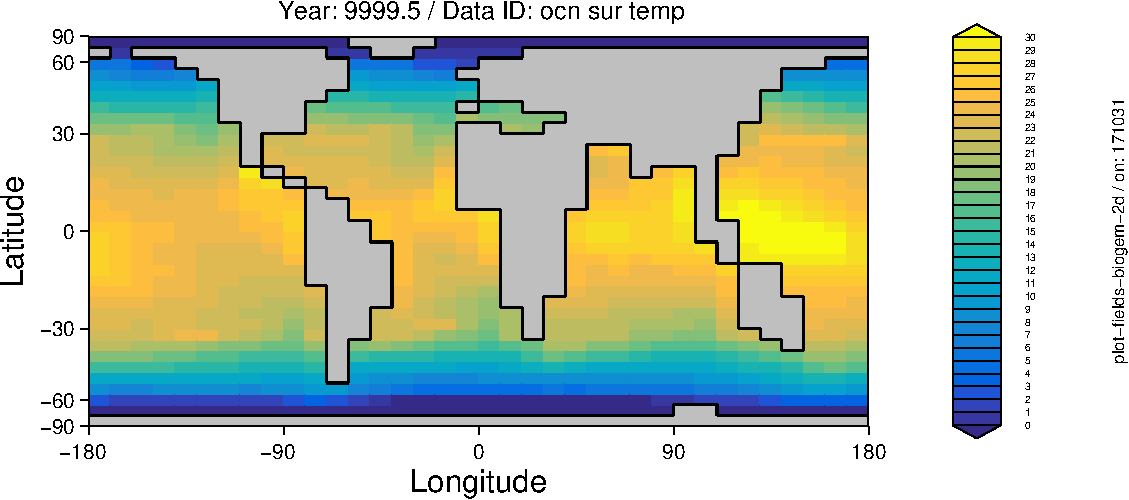
\includegraphics[scale=0.5]{example1a_171031.pdf}
\end{center}
\vspace{-4mm}
\caption{Example basic (default) surface temperature plot.}
\label{fig:example1a}
\end{figure}

For example:

\footnotesize
\vspace{-0pt}\begin{verbatim}
>> plot_fields_biogem_2d ...
('EXP1','','ocn_sur_temp','',9999.5,-1,16,'',1.0,0.0,30.0,30,'','','example1a');
\end{verbatim}\vspace{-0pt}
\normalsize
plots from the experiment \texttt{EXP1}, the variable \texttt{ocn\_sur\_temp} for time-slice \texttt{9999.5} (the mid-point time of the final year of a 10,000 year experiment). The color scale is from \texttt{0.0} to \texttt{30.0}, with no re-scaling (\texttt{1.0}), and \texttt{30} color intervals in the scale. The default \footnotesize\textsf{SETTINGS }\normalsize parameter file is used, and the default filename string replaced with \texttt{example1a}. The only other thing to note, is for parameter \texttt{PIK}, a value of \texttt{16} is set -- corresponding to the ocean surface. See Figure \ref{fig:example1a}.

Note that in this example, the   variable \texttt{ocn\_sur\_temp} is assumed. However, the model results variable \texttt{ocn\_sur\_temp} is not always saved in \textbf{BIOGEM} 2D netCDF output. If the requested variable, such as \texttt{ocn\_sur\_temp} does not exist, or is mis-spelt, \textbf{MATLAB} will pause and provide a warning. It will then list all the variables in the netCDF file that it can find and wait for a new variable name to be inputted. For instance, a variable that is always saved in \textbf{BIOGEM} 2D netCDF output is \texttt{atm\_temp} (surface air temperature) and could be substituted in the plot. Also note that time (the time-slice year to be plotted) is similarly handled -- if the specific time-slice value does not exist, a list of all possible time-slice years are provided and a substitute value requested as \textbf{MATLAB} pauses and wait for your input.

\begin{figure}[ht]
\begin{center}
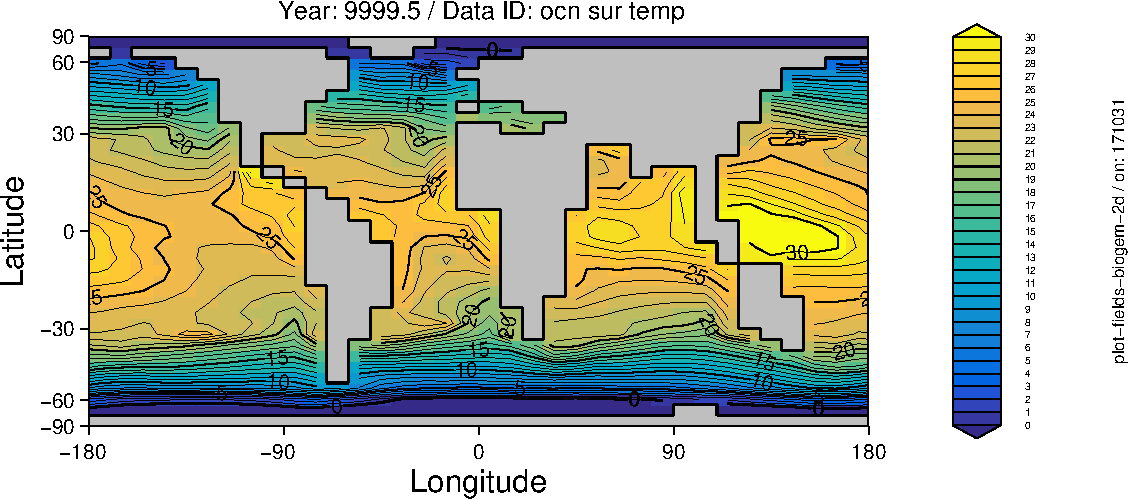
\includegraphics[scale=0.5]{example1b_171031.pdf}
\end{center}
\vspace{-4mm}
\caption{Example surface temperature plot, with contours.}
\label{fig:example1b}
\end{figure}

\vspace{4pt}
To add contours, in the default \footnotesize\textsf{SETTINGS }\normalsize parameter file (or a copied and re-named version thereof), adjust the following line:
\small
\vspace{-2pt}\begin{verbatim}
contour_plot = 'y';     % [ 'y']  OVERLAY CONTOUR PLOT?
\end{verbatim}\vspace{-2pt}
\normalsize
The results of this are shown in Figure \ref{fig:example1b}.

\pagebreak

Refinements to the contouring can be done by changing the lines:
\small
\vspace{-2pt}\begin{verbatim}
contour_mod = 1;        % [   1]  NUMBER OF COLOR INTERVALS PER CONTOR
contour_mod_label = 5;  % [   5]  NUMBER OF LABELED CONTOURS PER CONTOUR
contour_label = 'y';    % [ 'y']  LABEL CONTOURS?
contour_dashneg = 'n';  % [ 'n']  PLOT NEGATIVE CONTOURS DASHED?
\end{verbatim}\vspace{-2pt}
\normalsize
(these are the more commonly used refinements).

Here: \texttt{contour\_mod} determines how many color intervals per contour interval, which in the previous SST plot example, was \texttt{30}. So a value of \texttt{1} will give you 30 contours -- one every 1 degree C. And a value of \texttt{5} will give you 6 contours -- one each 5 degrees C.

\texttt{contour\_mod\_label} then determines whether you want the contours labelled or not. The answer (parameter value) to be the character \texttt{y} or \texttt{n}, as a string (i.e. in inverted commas). If you elect to have contour labels, \texttt{contour\_mod\_label} determines how frequently to label the contours. A value of \texttt{1} labels every single contour. A value of \texttt{2} labels every other contour. So for instance, if you set \texttt{contour\_mod=5} and \texttt{contour\_mod\_label=2} in the previous SST example, you get a contour every \texttt{5} degrees C, and a temperature label every \texttt{10} degrees C.

\vspace{4pt}
Alternatively, using 3d plotting, you could plot the ocean surface temperature field as follows:

\footnotesize
\vspace{-0pt}\begin{verbatim}
>> plot_fields_biogem_3d_k ...
('EXP1','','ocn_temp','',9999.5,-1,16,'',1.0,0.0,30.0,30,'','','example1c');
\end{verbatim}\vspace{-0pt}
\normalsize
The main things that change here are firstly the variable name -- now \texttt{ocn\_temp}, and secondly because this is a 3D ocean field, we need to specify what ocean model level we want to plot -- this is where the integer \texttt{16} comes in and corresponds to the input  \texttt{PIK}, as discussed earlier. The resulting plot will be identical to Figure \ref{fig:example1a}.

\vspace{4pt}
\item \textbf{Global zonal average temperature profile}

To keep with ocean temperature, we can use the \texttt{plot\_fields\_biogem\_3d\_i} function to plot the global zonal mean (lat-depth) profile (rather than horizontal, surface slice):

\footnotesize
\vspace{-0pt}\begin{verbatim}
>> plot_fields_biogem_3d_i ...
('EXP1','','ocn_temp','',9999.5,-1,0,'',1.0,0.0,30.0,30,'','','example2a');
\end{verbatim}\vspace{-0pt}
\normalsize
The only significant change as compared to before, is setting a \texttt{0} for input parameter \texttt{PIK} (again -- see earlier). The results is shown in Figure \ref{fig:example2a}.

\begin{figure}[ht]
\begin{center}
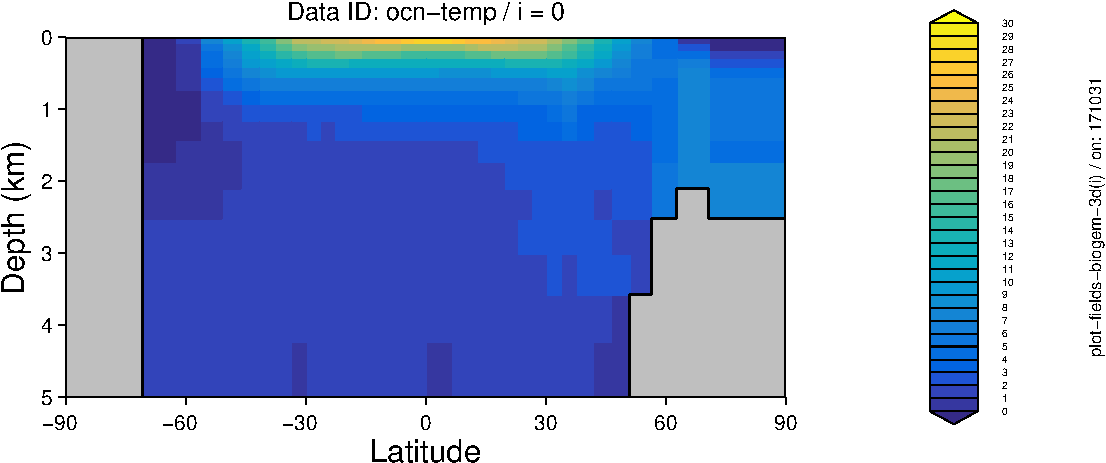
\includegraphics[scale=0.5]{example2a_171031.pdf}
\end{center}
\vspace{-4mm}
\caption{Zonal mean global ocean temperature profile.}
\label{fig:example2a}
\end{figure}

\vspace{4pt}
\item \textbf{Pacific dissolved oxygen profile}

As per choosing ocean levels (\texttt{k}-values) in the lon-lat plotting, you can also specify a specific longitude for creating a lat-depth section rather than calculating and plotting a global zonal mean. e.g. Figure \ref{fig:example3a} was created by\footnote{Also turning on the contour plotting.}:

\footnotesize
\vspace{-0pt}\begin{verbatim}
>> plot_fields_biogem_3d_i ...
('EXP1','','ocn_O2','',9999.5,-1,10,'',1.0E-6,0.0,300.0,30,'','','example3a');
\end{verbatim}\vspace{-0pt}
\normalsize
The chosen section is somewhere in the Pacific, along a line of longitude (whatever corresponds to \texttt{i=10} on this \textbf{muffin} model grid ... I guess about 165W ...). Here, the variable to be plotted has also been changed -- \texttt{ocn\_O2}\footnote{You'll need a biogeochemsitry enabled \textit{base-config}}. Because the units of dissolved oxygen are much smaller than for temperature (in degrees C),  the plotted scale has also been changed -- from 0 to 300 \(\mu mol kg^{-1}\) rather than the netCDF variable units of \(mol kg^{-1}\). To achieve this re-scaling, a units scaling value of \texttt{1.0E-6} is specified for parameter \texttt{PCSCALE}.\footnote{Note that the scaling specified is as the new units relative to the old units -- here, \(\mu mol kg^{-1}\) relative to \(mol kg^{-1}\) and hence \(10^{-6}\). ALSO NOTE that \textbf{Panoply} does it the other way around ... :(}

\begin{figure}[ht]
\begin{center}
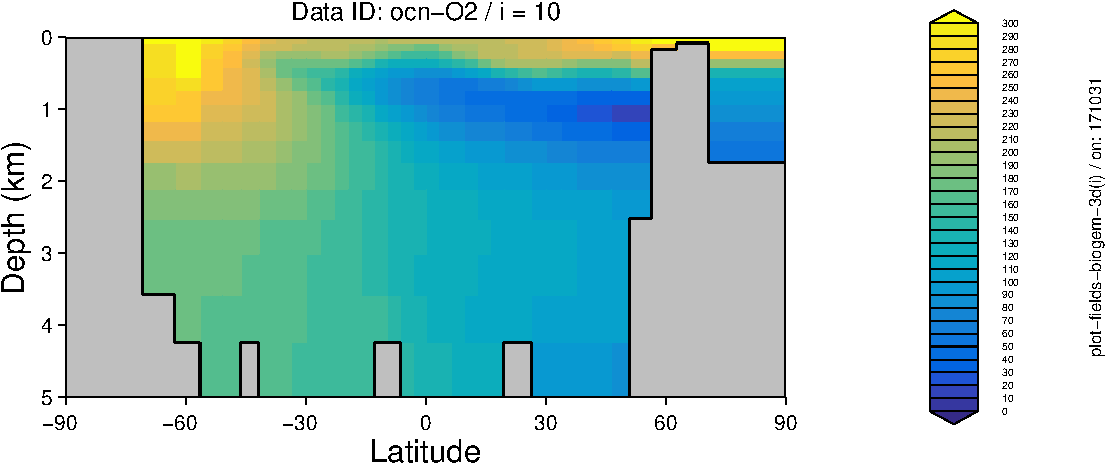
\includegraphics[scale=0.5]{example3a_171031.pdf}
\end{center}
\vspace{-4mm}
\caption{Ocean oxygen profile on a Pacific transect.}
\label{fig:example3a}
\end{figure}

\vspace{4pt}
\item \textbf{Atlantic zonal mean dissolved oxygen profile}

So far, with the exception of plotting a gridded color field \uline{and} a contoured field at the same time, all these examples can also be done in \textbf{Panoply}. One difference, is the ability in the \textbf{muffinplot} suite of \textbf{MATLAB} functions to apply masks -- isolating geographical regions or even single points. In the \footnotesize\textsf{MASKS }\normalsize directory, are a series of example ASCII mask files, mostly for the 2 (8- and 16-level ocean) modern published configurations of \textbf{muffin}. For instance, \footnotesize\textsf{mask\_worjh2\_AtlanticALL.dat }\normalsize has all the grid points in the entire Atlantic basin assigned a value of \texttt{1}, with \texttt{0} everywhere else. If we apply this first to the surface ocean dissolved oxygen field:

\footnotesize
\vspace{-0pt}\begin{verbatim}
>> plot_fields_biogem_3d_k ...
('EXP1','','ocn_O2','',9999.5,-1,16,'mask_worjh2_AtlanticALL.dat',1.0E-6,0.0,300.0,30,
... '','','example4a');
\end{verbatim}\vspace{-0pt}
\normalsize
we obtain Figure \ref{fig:example4a}.

\begin{figure}[ht]
\begin{center}
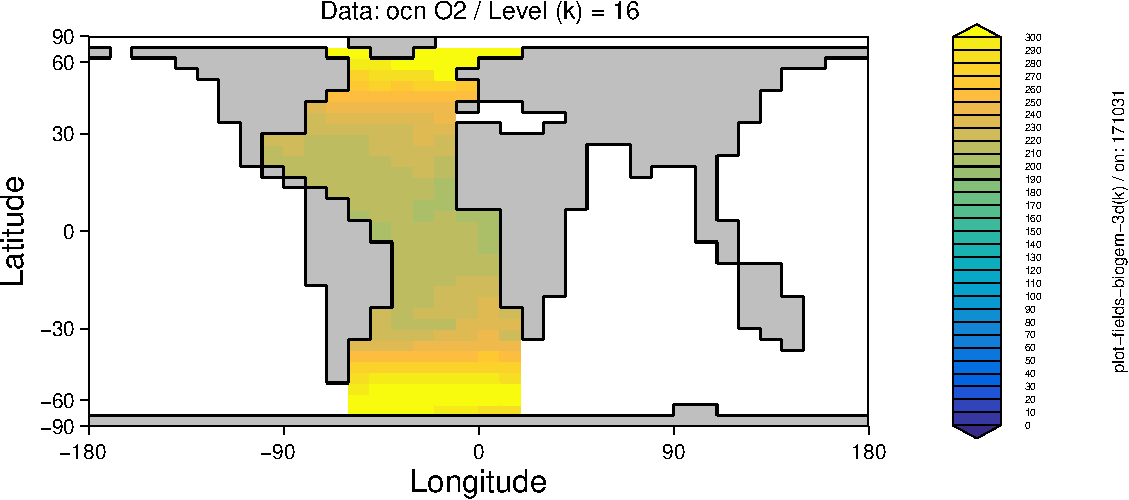
\includegraphics[scale=0.5]{example4a_171031.pdf}
\end{center}
\vspace{-4mm}
\caption{Distribution of surface ocean dissolved  oxygen in the Atlantic.}
\label{fig:example4a}
\end{figure}

Here, it is clear how the masked has been applied and all the ocean falling outside of the mask is plotted as white (no data).

We can also apply a mask field to the zonal average plot:

\footnotesize
\vspace{-0pt}\begin{verbatim}
>> plot_fields_biogem_3d_i ...
('EXP1','','ocn_O2','',9999.5,-1,0,'mask_worjh2_AtlanticALL.dat',1.0E-6,0.0,300.0,30,
... '','','example4b');
\end{verbatim}\vspace{-0pt}
\normalsize
(Figure \ref{fig:example4b})

\begin{figure}[ht]
\begin{center}
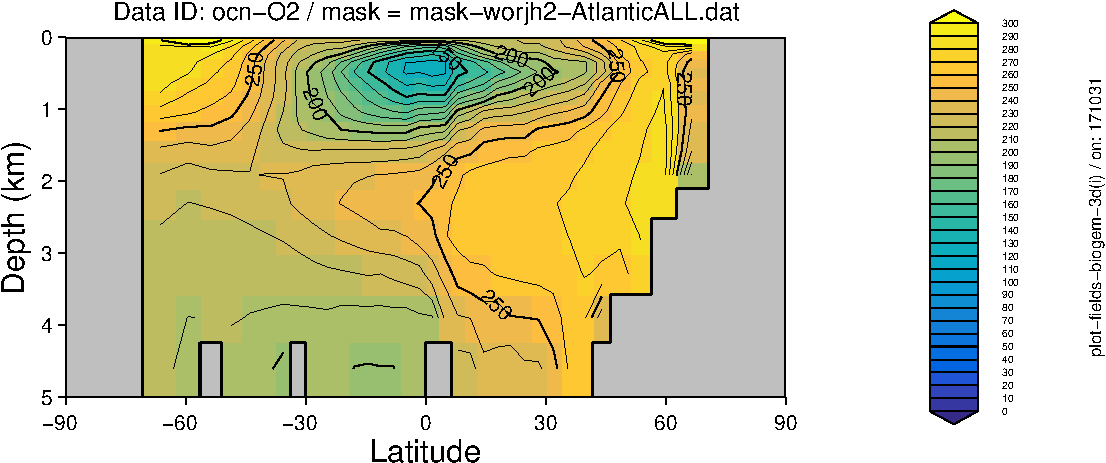
\includegraphics[scale=0.5]{example4b_171031.pdf}
\end{center}
\vspace{-4mm}
\caption{Mean zonal ocean oxygen profile in the Atlantic.}
\label{fig:example4b}
\end{figure}

\end{enumerate}

%------------------------------------------------

\subsection{Difference maps}



%------------------------------------------------

\subsection{Model-data and data maps}



%------------------------------------------------

\subsection{Example plotting suite}

An set of \textbf{MATLAB} \footnotesize\textsf{m-file }\normalsize functions are provided that define a series of different generic and basic experiment analysis and plottings, with \footnotesize\textsf{make\_analysis\_ALL.m }\normalsize provided as a template for carrying them all out in one go. Obviously, the individual aggregate plotting functions can be edited, added to, or with unwanted or irrelevant plots, commented out or deleted -- treat these all simply as templates for developing your own analysis strategy (as well as viewing the associated configuration files as illustrations of the function/use of some of the different further plotting options\footnote{Also covered in a subsequent sub-sub-section.}).

The aggregate plotting functions are as follows:

\begin{enumerate}[noitemsep]

\vspace{1pt}
\item \footnotesize\textbf{\textsf{fun\_make\_analysis\_phys.m}}\normalsize \\This encompasses a basic set of analyses of ocean circulation and climatology.
\\The script is written as a \textit{function}, and requires just two parameters to be passed as input:
\begin{enumerate}[noitemsep]
\setlength{\itemindent}{.2in}
\item The experiment name.
\item The (mid-point of the) year of the time-slice to plot.
\end{enumerate}
In the example of an experiment called \texttt{'EXP1'}, and plotting the last annual time-slice (\texttt{9999.5}) from a 10,000 year model run, the function is hence called:
\vspace{-2pt}\begin{verbatim}
fun_make_analysis_phys('EXP1',9999.5);
\end{verbatim}\vspace{-2pt}

\vspace{1pt}
\item \footnotesize\textbf{\textsf{fun\_make\_analysis\_geo.m}}\normalsize \\This encompasses a basic set of analyses of ocean (abiotic) geochemistry and ocean acidification related variables and metrics.

\vspace{1pt}
\item \footnotesize\textbf{\textsf{fun\_make\_analysis\_bio.m}}\normalsize \\This encompasses a basic set of analyses of marine biological fluxes and biologically related properties.

\vspace{1pt}
\item \footnotesize\textbf{\textsf{fun\_make\_analysis\_ALL.m}}\normalsize
\\Aggregates all the above functions (i.e., calls all 3).
\end{enumerate}

\vspace{2pt}
To run these example analysis -- either copy all the files contained in the \footnotesize\textsf{EXAMPLES }\normalsize subdirectory, to your working directory (e.g. \footnotesize\textsf{RESULTS }\normalsize as per the previous example). Then type e.g..\footnote{Note that if you did not run with ocean biogeochemsitry (but rather climate-only), not all the plotting functions will run and you will have to restrict this default analysis to: \texttt{fun\_make\_analysis\_phys('EXP1',9999.5);}}

\vspace{-2pt}\begin{verbatim}
fun_make_analysis_ALL('EXP1',9999.5);
\end{verbatim}\vspace{-2pt}

\noindent OR, add the path to the \footnotesize\textsf{EXAMPLES }\normalsize subdirectory, e.g.
\vspace{-2pt}\begin{verbatim}
addpath('Y:\_git\muffinplot\EXAMPLES');
\end{verbatim}\vspace{-2pt}
but obviously depending on quite where you installed \textbf{muffinplot}.

%------------------------------------------------

\subsection{Further refinements}

A number of additional options for exerting finer control over the plotting are provided as a block of parameters and (default) values in the m-file itself, in a section immediately after the commented help and change-log at the start of the m-file. Not all the options are relevant to all the plotting functions\footnote{See 'help' on a specific plotting function for details of the relevant options in the parameter block.}, but the full list (and then defaults in brackets \texttt{[]}) is as follows:

\vspace{2pt}
{\small \begin{enumerate}
\item \texttt{lon\_min = -180;         [-180]  STARTING LONGITUDE FOR X-AXIS}
\\ Sets the longitude of the left-hand edge of the plot.
\item \texttt{delta\_lon = 90;         [  90]  INCREMENT OF LONGITUDE ON X-AXIS}
\\ Sets the longitude tick increment.
\item \texttt{contour\_plot = 'n';     [ 'n']  OVERLAY CONTOL PLOT?}
\\ Overlay line contours on the color block plot?
\item \texttt{contour\_mod = 2;        [   2]  NUMBER OF COLOR INTERVALS PER CONTOR}
\\ Number of color graduations per line contour.
\item \texttt{contour\_mod\_label = 4;  [   4]  NUMBER OF LABELED CONTOURS PER CONTOUR}
\\ Number of color graduations per labeled line contour.
\item \texttt{contour\_label = 'y';    [ 'y']  LABEL CONTOURS?}
\\ Label the line contours (frequency of labeled contours set by \texttt{contour\_label}.
\item \texttt{contour\_noneg = 'n';    [ 'n']  RESTRICT DATA PLOTTED TO > 0.0?}
\\ Restrict the plotted values to non-negative? (Can be useful if slightly negative values exist as can occur during tracer transport associated with large concentration gradients.)
\item \texttt{plot\_log10 = 'n';       [ 'n']  PLOT LOG10 OF THE DATA}
\\ Plot data values as log10(value)?
\item \texttt{contour\_zero = 'y';     [ 'y']  PLOT ZERO CONTOUR}
\\ Plot the zero contour?
\item \texttt{colorbar\_old = 'n';     [ 'n']  PLOT 'OLD' COLORBAR}
\\ Plot old style colorbar.
\item \texttt{data\_offset = 0.0;      [ 0.0]  data offset (273.15 for K -> C)}
\\ Introduce a data offset? This is useful for example for converting K to degrees C (removing the K value of 0 degrees C).
\item \texttt{data\_ij = 'n';          [ 'n']  DATA as (i,j)?}
\\ Overlay data in the form of (i,j) locations rather than longitude,latitude?
\item \texttt{data\_ijk = 'n';          [ 'n']  DATA as (i,j,k)?}
\\ Overlay data in the form of (i,j,k) locations rather than longitude, latitude, depth?
\item \texttt{data\_ij\_mean = 'n';     [ 'n']  average DATA by cell?}
\\ Average overlay data per \textit{c}GENIE grid cell rather than plotting raw locations.
\item \texttt{data\_ijk\_mean = 'n';     [ 'n']  average DATA by cell?}
\\ Average overlay data per \textit{c}GENIE grid cell rather than plotting raw locations.
\item \texttt{data\_size = 25.0;       [25.0]  SIZE OF OVERLAY DATA POINTS}
\\ Size of the overlay data points.
\item \texttt{data\_anomoly = 'n';     [ 'n']  PLOT AS MODEL-DATA ANOMOLY ONLY?}
\\ Plot data locations with the model-data anomaly rather than data value?
\item \texttt{data\_only = 'n';        [ 'n']  PLOT ONLY DATA (no model values)?}
\\ Plot only the overlay data locations (and not any model data)?
\item \texttt{data\_site = 'n';        [ 'n']  PLOT DATA AS SITES (no data values)?}
\\ Plot labeled site locations (no data value fill).
\item \texttt{plot\_land = 'n';        [ 'n']  PLOT DATA OVER LAND?}
\\ Plot data locations lying over land on the \textit{c}GENIE grid (rather than screen out)?
\item \texttt{data\_uv = 'n';          [ 'n']  overlay (u,v) velocity data?}
\\ Overlay ocean current fields.
\item \texttt{data\_uv\_scale = 1.0;    [ 1.0]  scaling factor for vector length}
\\ Scaling factor for velocity vectors.
\item \texttt{plot\_opsi = '';         [  '']  PLOT OVERTURNING STREAMFUNCTION (basin)?}
\\ Plot overturning streamfunction overlay?
\item \texttt{plot\_opsi\_min = -15;    [ -15]; plot\_opsi\_max = +15;    [ +15];
plot\_opsi\_dminor = 1;   [   1]; plot\_opsi\_dmajor = 5;   [   5] }
\\ Controls on min, max and (major and minor) contor intervals.
\item \texttt{dscrsz = 0.60;          [0.60]  FRACTIONAL FIGURE WINDOW SIZE}
\\ Adjustment factor of the fractional size (compared to the screen) of the figure window.
\end{enumerate}}
\vspace{2pt}

\subsubsection{Further refinements: Examples}

Examples:
\begin{enumerate}
\item To plot the positions (and labels) of data locations:
\\ {\small \texttt{plot\_fields\_biogem\_3d\_k('cgenie\_output','120926.SPIN','',49999.5,-1,'ocn\_temp','','',\\16,1.0,10.0,40.0,30,'','sites.dat')}}
\\ where the experiment name is \texttt{120926.SPIN}, the mapped variable is \texttt{ocn\_temp} (although no model field need be plotted -- set by an option in the plotting function itself, and the file of data locations is \texttt{sites.dat}.
\end{enumerate}

\begin{figure}[ht]
\begin{center}
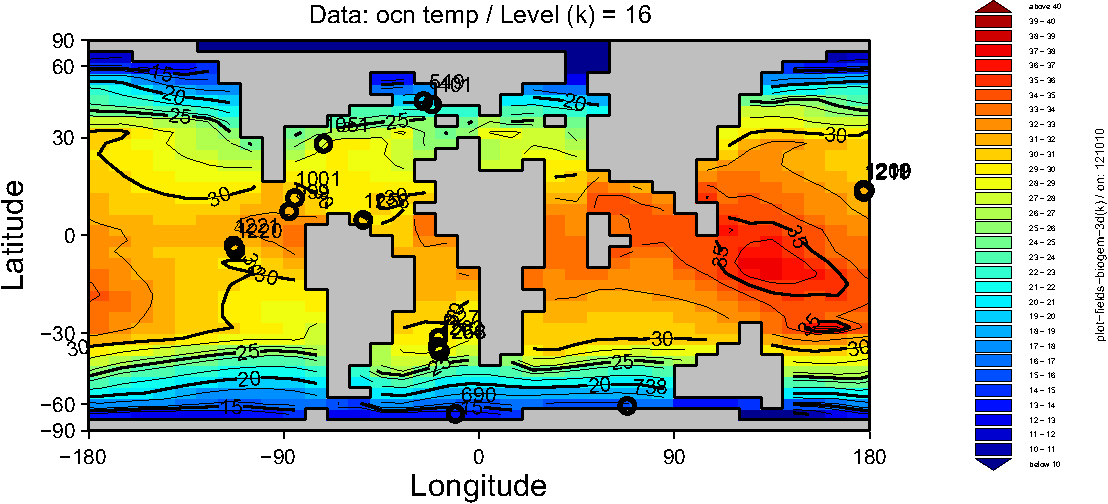
\includegraphics[scale=0.75]{cgenie_datalocations.pdf}
\end{center}
\caption{Paleocene-Eocene deep-sea sediment drill locations together with a contour-overlain map of surface temperature.}
\label{fig:cgenie_datalocations}
\end{figure}

%------------------------------------------------

\section{Sediment model output analysis}

%----------------------------------------------------------------------------------------
%----------------------------------------------------------------------------------------
%----------------------------------------------------------------------------------------
%       CHAPTER 16
%----------------------------------------------------------------------------------------

\cleardoublepage

\chapterimage{big-data.jpg} % Chapter heading image

\chapter{muffindata}\label{ch:muffindata}

\hfill \break

%------------------------------------------------
\newpage
%------------------------------------------------

\section{(none)}

%----------------------------------------------------------------------------------------
%----------------------------------------------------------------------------------------
%----------------------------------------------------------------------------------------
%       CHAPTER 17
%----------------------------------------------------------------------------------------

\cleardoublepage

%\chapterimage{xxx} % Chapter heading image

\chapter{xxx}\label{ch:17}

\hfill \break

%------------------------------------------------
\newpage
%------------------------------------------------

\section{(none)}

%----------------------------------------------------------------------------------------
%----------------------------------------------------------------------------------------
%----------------------------------------------------------------------------------------
%       CHAPTER 18
%----------------------------------------------------------------------------------------

\cleardoublepage

%\chapterimage{xxx} % Chapter heading image

\chapter{xxx}\label{ch:18}

\hfill \break

%------------------------------------------------
\newpage
%------------------------------------------------

\section{(none)}

%----------------------------------------------------------------------------------------
%----------------------------------------------------------------------------------------
%----------------------------------------------------------------------------------------
%       CHAPTER 19
%----------------------------------------------------------------------------------------

\cleardoublepage

\chapterimage{ch-howto.png} % Chapter heading image

\chapter{HOW-TO (technical)}\label{ch:how-to-technical}

\hfill \break

%------------------------------------------------
\newpage
%------------------------------------------------

\section{(none)}

%----------------------------------------------------------------------------------------
%----------------------------------------------------------------------------------------
%----------------------------------------------------------------------------------------
%       CHAPTER 20
%----------------------------------------------------------------------------------------

\cleardoublepage

\chapterimage{ch-howto.png} % Chapter heading image

\chapter{HOW-TO (experiment)}\label{ch:how-to-experiment}

\hfill \break

%------------------------------------------------
\newpage
%------------------------------------------------

\section{(none)}

%----------------------------------------------------------------------------------------
%----------------------------------------------------------------------------------------
%----------------------------------------------------------------------------------------
%       CHAPTER 21
%----------------------------------------------------------------------------------------

\cleardoublepage

\chapterimage{muffin_planet.jpg} % Chapter heading image

\chapter{cookie Development}\label{ch:model-code}

\hfill \break

%------------------------------------------------
\newpage
%------------------------------------------------

\section{(none)}

%----------------------------------------------------------------------------------------
%----------------------------------------------------------------------------------------

%----------------------------------------------------------------------------------------
%----------------------------------------------------------------------------------------

\backmatter

%----------------------------------------------------------------------------------------
%       INDEX
%----------------------------------------------------------------------------------------

%\cleardoublepage
%\phantomsection
%\setlength{\columnsep}{0.75cm}
%\addcontentsline{toc}{chapter}{\textcolor{ocre}{Index}}
%\printindex

%----------------------------------------------------------------------------------------

\end{document}

%----------------------------------------------------------------------------------------
%----------------------------------------------------------------------------------------
%----------------------------------------------------------------------------------------